% \includeonly{lec_23}

\documentclass[numberindividually, numberwithin=section, empheqoverload,filemanagement]{hrflecture}
\renewcommand*{\sectionformat}{\textsection\thesection\autodot\enskip}
\addtokomafont{section}{\mdseries}
\let\Mat\relax
\DeclareMathOperator{\Mat}{M}
\let\angleold=\angle
\renewcommand*{\angle}{\sphericalangle}
\DeclarePairedDelimiterXPP{\aglacoursematrices}[3]{\Mat_{#1\times #2}}{\lparen}{\rparen}{}{#3}
\let\matrices\aglacoursematrices

\DeclareMathOperatorWithDelimiter-{\aglacoursetranspose}[1,1]{\vphantom{#1}^t}{\lparen}{\rparen}{#1}
\let\transpose\aglacoursetranspose

\newtheorem{beweisbehauptung}{Behauptung}[satz]
\renewcommand\thebeweisbehauptung{\arabic{beweisbehauptung}}
\newtheorem*{lemmastrich}{Lemma 1'}

\setlength{\marginparpush}{1cm}
\WarningFilter*{latex}{Marginpar on page \thepage\space moved}




\subject{Vorlesungsmitschrift}
\title{AGLA \texorpdfstring{\Romannum{2}}{2}}
\subtitle{Prof.~Dr.~Damaris~Schindler}
\date{Auf dem Stand vom \today}
\author{Henry Ruben Fischer}

\begin{document}
\maketitle

\newpage
\textbf{Disclaimer}
\vspace{1cm}

Nicht von Professor Schindler durchgesehene Mitschrift, keine Garantie auf Richtigkeit ihrerseits.

% \newpage
\tableofcontents
% \newpage
\listoflectures
\listoffiles


\automark{section}
% some more adjustments
\makeatletter
\renewtheorem{satz}[lemma]{Satz}
\renewtheorem{korollar}[lemma]{Korollar}
\makeatother
% Begin of lectures
% !TEX root = ./Vorlesungsmitschrift AGLA 2.tex 
\chapter{Affine Geometrie}
\lecture{1}{Di 21.04. 10:15}{}
\section{Was ist ein affiner Raum?}
\begin{beispiel}[aus der AGLA \Romannum{1}]
    \( \reals^2, \reals^3 \). 
    In diesen Räumen gibt es einen ausgezeichneten \enquote{Usprung}.
\end{beispiel}
\begin{frage*}
    Wie könne wir eine affine Ebene / affine Röume modellieren, wobei alle Punkte gleichberechtigt sind?
\end{frage*}
\begin{idee*}
    Verwende affine Unterräume.
\end{idee*}
\begin{beispiel}\label{affiner_unterraum}
    Sei \( K \) ein Körper, \( V \) ein \( K \)-Vektorraum, \( W\subseteq V \) ein Untervektorraum und \( v\in V \). 
    Wir nennen \( X=v+W \) einen affinen Unterraum von \( V \). 
    \( X \) ist im Allgemeinen selbst kein Vektorraum unter der Addition in \( V \), aber \( W \) \enquote{operiert} auf \( X \).
    \begin{figure}[H]
        \centering
        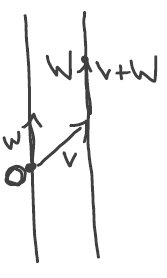
\includegraphics[width=0.2\linewidth]{figures/affiner_unterraum}
        \label{fig:affiner_unterraum}
    \end{figure}
    
    Für \( w\in W \) definieren wir die Abbildung
    \begin{align*}
        \tau_w\maps \begin{aligned}[t] 
            X&\to X\\
            p &\mapsto p+w.
        \end{aligned}
    \end{align*}
    \begin{figure}[H]
        \centering
        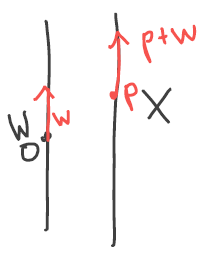
\includegraphics[width=0.2\linewidth]{figures/tau_w}
        \label{fig:tau_w}
    \end{figure}
    Sei
    \begin{align*}
        \Bij(X)=\Set{f\maps X\to X, f \text{ ist bijektiv}}.
    \end{align*}
    Dann ist \( \tau_w\in \Bij(X) \) für alle \( w\in W \).
\end{beispiel}
\begin{bemerkung*}
    \( \Bij(X) \) ist eine Gruppe unter Verkettung von Abbildung. 
    Wir erhalten eine Abbildung
    \begin{align*}
        \tau\maps \begin{aligned}[t] 
            W &\to \Bij(X)\\
            w &\mapsto \tau_w.
        \end{aligned}
    \end{align*}
\end{bemerkung*}
\begin{lemma}
    Die Abbildung \( \tau \) ist ein Gruppenhomomorphismus.
\end{lemma}
\begin{proof}
    Seien \( w, w' \in W \)
    Dann
    \begin{align*}
        \tau_w\circ \tau_{w'}\maps \begin{aligned}[t] 
            X &\to X\\
            p &\mapsto p+\underbracket{w'+w},
        \end{aligned}
    \end{align*}
    also
    \begin{align*}
        \tau(w)\circ \tau(w')=\tau_w\circ \tau_{w'}=\tau_{w+w'}=\tau(w+w').
    \end{align*}
    
\end{proof}
Es gilt noch mehr:

\textcolor{Turquoise}{für \( p, q \in X \)} besteht genau ein \( w\in W \) mit \( \tau_w(p)=q \).

\begin{figure}[H]
    \centering
    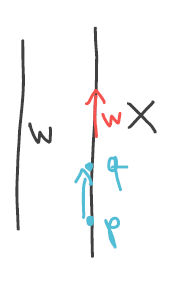
\includegraphics[width=0.2\linewidth]{figures/tau_w_bijektion}
    \label{fig:tau_w_bijektion}
\end{figure}

\section*{Gruppenoperationen}
\begin{beispiel}\label{d_3}
    Betrachte ein gleichseitiges Dreieck \( D \) und Spiegelungen / Drehungen die \( D \) auf sich selbst abbilden.

    \begin{figure}[H]
        \centering
        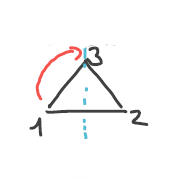
\includegraphics[width=0.2\linewidth]{figures/d_3}
        \label{fig:d_3}
    \end{figure}
    Diese formen eine Gruppe (welche?) und \enquote{operieren} auf \( D \).
\end{beispiel}
\begin{definition}
    Sei \( X \) eine Mege und \( G \) eine Gruppe. 
    Eine Operation von \( G \) auf \( X \) ist ein Homomorphismus von Gruppen
    \begin{align*}
        \tau\maps \begin{aligned}[t] 
            G&\to \Bij(X)\\
            g&\mapsto \tau_g.
        \end{aligned}
    \end{align*}
\end{definition}
\begin{bemerkung*}
    \( \tau \) ist ein Homomorphismus \dh \tforall \( g, g' \in G \)
    \begin{align*}
        \tau_g\circ \tau_{g'}=\tau_{gg'}.
    \end{align*}
    
    Für \( x\in X \) nennen wir
    \begin{align*}
        G(x)=\Set{\tau_g(x)|g\in G}
    \end{align*}
    die Bahn von \( x \) unter \( G \).
\end{bemerkung*}
\begin{beispiel}\label{operation:beispiele}
    \begin{eigenschaftenenumerate}
        \item \label{operation:beispiele:linkstranslation} Sei \( G \) eine Gruppe und \( X=G \) die Linkstranslation \( l\maps \begin{aligned}[t] 
            G&\to \Bij(G)\\
            g&\mapsto l_g
        \end{aligned} \) mit \( l_g(x)=gx \quad\forall x\in G \) ist eine Gruppenoperation von \( G \) auf sich selbst.
        
        \item \label{operation:beispiele:konjugation}\begin{align*}
            k\maps \begin{aligned}[t] 
                G &\to \Bij(G)\\
                g &\mapsto kg
            \end{aligned}
        \end{align*}
        mit \( k_g(x)=gx\inv{g} \quad\forall x\in G \) ist eine Gruppenoperation.
    \end{eigenschaftenenumerate}
\end{beispiel}
\thref{operation:beispiele}~\ref{operation:beispiele:konjugation}
\begin{frage*}
    Sei \( \tau\maps G\to \Bij(x) \) eine Gruppenoperation, \( x,y\in X \). 
    Wann gibt es ein \( g\in G \) mit \( \tau_g(x)=y \)?
    \begin{figure}[H]
        \centering
        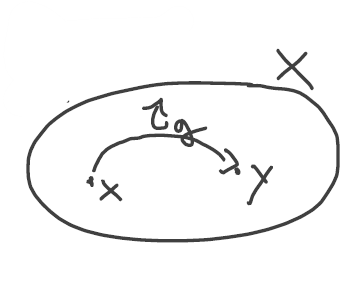
\includegraphics[width=0.5\linewidth]{figures/einfach_transitiv}
        \label{fig:einfach_transitiv}
    \end{figure}
    
\end{frage*}

\begin{definition*}
    Sei \( \tau\maps G\to \Bij(X) \) eine Gruppenoperation von \( G \) auf \( X \). 
    Wir nennen \( \tau \) \emph{einfach transitiv}, wenn \tforall \( x,y\in X \) \emph{genau ein} \( g\in G \) besteht mit
    \begin{align*}
        \tau_g(x)=y.
    \end{align*}
\end{definition*}
\begin{beispiel*}
    \begin{itemize}
        \item Die Gruppenoperation aus \thref{d_3} ist \emph{nicht} einfach transitiv
        \begin{figure}[H]
            \centering
            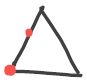
\includegraphics[width=0.2\linewidth]{figures/d_3_nicht_einfach_transitiv}
            \label{fig:d_3_nicht_einfach_transitiv}
        \end{figure}
        
        \item Die Linkstranslation aus \thref{operation:beispiele}~\ref{operation:beispiele:linkstranslation} ist immer einfach transitiv.
    \end{itemize}
\end{beispiel*}
Zurück zum \thref{affiner_unterraum} (\( V \) \( K \)-Vektorraum, \( W\subseteq V \) Untervektorraum, \( v\in V \), \( X=v+W \))

Wir haben Translationen definiert
\begin{align*}
    \tau\maps \begin{aligned}[t] 
        W&\to \Bij(X)\\
        x&\mapsto \tau_w
    \end{aligned}
\end{align*}
mit \( \tau_w\maps X\to X \), \( p\mapsto p+w \). 
\( \tau \) ist eine einfach transitive Gruppenoperation von \( W \) auf \( x \).

\begin{figure}[H]
    \centering
    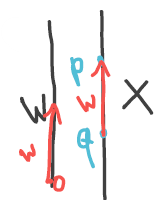
\includegraphics[width=0.2\linewidth]{figures/affiner_unterraum_einfach_transitive_gruppenoperation}
    \label{fig:affiner_unterraum_einfach_transitive_gruppenoperation}
\end{figure}

\begin{definition*}
    Sei \( K \) ein Körpr. 
    Ein affiner Raum über \( K \) ist ein Tripel \( (X, T(X), \tau ) \) mit
    \begin{itemize}
        \item \( X\neq \emptyset \) eine Menge 
        \item \( T(X) \) ein \( K \)-Vektorraum 
        \item \( \tau\maps T(x)\to \Bij(X) \) eine einfach transitive Gruppenoperation
    \end{itemize}
\end{definition*}
\begin{konvention*}
    \( X=\emptyset \) ohne Spezifikation von \( T(X) \), \( \tau \) nennen wir auch einen affinen Raum.
\end{konvention*}
\begin{figure}[H]
    \centering
    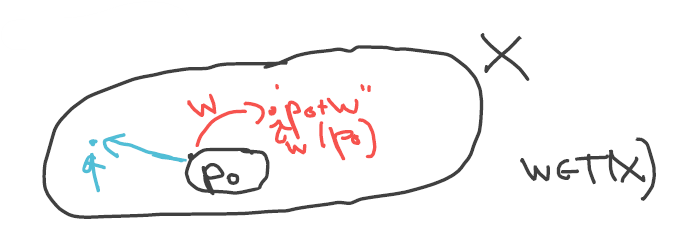
\includegraphics[width=0.5\linewidth]{figures/affiner_raum}
    \label{fig:affiner_raum}
\end{figure}
\begin{definition*}
    Sei \( (X,T(X),\tau) \) in affiner Raum über einem Körper \( K \). 
    Dann nennen wir \( \dim_K T(X) \) die Dimension von \( X \), schreiben auch \( \dim X \).
     
    Ist \( \dim X=1 \) \bzw \( \dim X=2 \), dann nennen wir \( X \) eine affine Gerade \bzw affine Ebene.
\end{definition*}

Sei \( (X, T(X), \tau) \) in affiner Raum, \( p,q\in X \). Dann \( \existsone t\in T(X) \) mit \( \tau_t(p)=q \).

\textcolor{Turquoise}{Schreibe \( \vv{pq}=t\in T(X) \) als \( \tau_{\vv{pq}}(p)=q \).}
\begin{figure}[H]
    \centering
    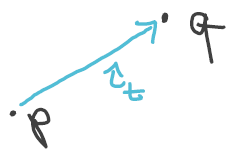
\includegraphics[width=0.2\linewidth]{figures/vektornotation}
    \label{fig:vektornotation}
\end{figure}
Wir erhalten eine Abbildung
\begin{align*}
    X\times X&\to T(X)\\
    (p,q)&\mapsto \vv{pq}.
\end{align*}
\begin{frage*}
    Welche Eigenschaften hat die Abbildung \( (p,q)\mapsto \vv{pq} \) in einem allgemeinen affinen Raum?
\end{frage*}
\begin{lemma}\label{vektoren_funzen_richtig}
    Sei \( X \) ein affiner Raum, \( p,q,r\in X \). Dann gilt \( \vv{pq}+\vv{qr}=\vv{pr} \).
\end{lemma}
\begin{figure}[H]
    \centering
    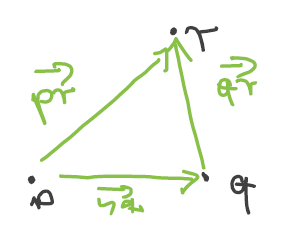
\includegraphics[width=0.3\linewidth]{figures/vektoren_funzen_richtig}
    \label{fig:vektoren_funzen_richtig}
\end{figure}
\begin{proof}
    \( \tau\maps T(X)\to \Bij(X) \) ist ein Homomorphismus. 
    Also gilt \( \tau_{\vv{qr}}\circ \tau_{\vv{pq}}=\tau_{\vv{pq}+\vv{qr}} \). 
    Es gilt damit \( \tau_{\vv{pq}+\vv{qr}}(p)=r \). 
    Also \( \vv{pq}+\vv{qr}=\vv{pr} \).    
\end{proof}

\section{Affine Abbildungen}
Seien \( V,W \) \( K \)-Vektorräume.
In der AGLA \Romannum{1}: lineare Abbildungen
\begin{align*}
    F\maps V\to W,
\end{align*}
\dh \( F \) respektiert die Vektorraum-Struktur
\begin{align*}
    F(v_1+v_2)=F(v_1)+F(v_2)\quad\forall v_1,v_2\in V\\
    F(\lambda v)=\lambda F(v)\quad \forall\lambda\in K \forall v \in V.
\end{align*}
\begin{frage*}
    Was sind natürliche Abbildungen zwischen affinen Räumen?
\end{frage*}
Seien \( X, Y \) affine Räume über einem Körper \( K \).

Seien \( X, Y \) affine Räume über einem Körper \( K \)
\begin{figure}[H]
    \centering
    \includegraphics[width=0.8\linewidth]{figures/affine_Abbildungen}
    \label{fig:affine_Abbildungen}
\end{figure}
\begin{align*}
    \textcolor{Turquoise}{\vertrelate{\vertni}{T(X)}{\vv{pq}}\rightsquigarrow\vertrelate{\vertni}{T(Y)}{\vv{f(p)f(q)}}}.
\end{align*}
\begin{definition*}
    Wir nennen eine Abbildung \( f\maps X \to Y \) affin, wenn s eine \( K \)-lineare Abbildung \( F\maps T(X)\to T(Y) \) gibt, sodass \tforall \( p,q\in X \) gilt
    \begin{align*}
        \vv{f(p)f(q)}=F(\vv{pq}).
    \end{align*}
\end{definition*}
\begin{bemerkung*}
    \begin{eigenschaftenenumerate}
        \item Es gibt im Allgemeinen verschiedene affine Abbildungen \( f\maps X \to Y \), die zur gleichen linearen Abbildung \( F\maps T(X)\to T(Y) \) gehören.
        \item Sei \( p_0 \in X \) fest und \( f\maps X \to Y \) affin.
        
        Für \( q\in X \) gilt
        \begin{align*}
            f(q)\begin{aligned}[t] 
                &=\tau_{\vv{f(p_0)f(q)}}(f(p0))\\
            &=\tau_{F(\vv{p_0 q})}(f(p0)).
            \end{aligned}
        \end{align*}
        Also bestimmen \( f(p_0) \) und \( F \) zusammenen die Abbildung \( f\maps X\to Y \).
    \end{eigenschaftenenumerate}


\end{bemerkung*}
\begin{beispiel*}
    Seien \( V,W \) \( K \)-Vektorräume
    \begin{align*}
        X=(V,V,\tau),\quad Y=(W,W,\tau).
    \end{align*}
    Eine affine Abbildung \( f\maps V\to W \) ist eindeutig bestimmt durch \( f(0) \) und eine lineare Abbildung \( F\maps V\to W \). Es gilt
    \begin{align*}
        f(v)=\textcolor{Goldenrod}{f(0)}+\textcolor{LimeGreen}{F(v)}\quad\forall \textcolor{LimeGreen}{v} \in V.
    \end{align*}
\end{beispiel*}
\begin{figure}[H]
    \centering
    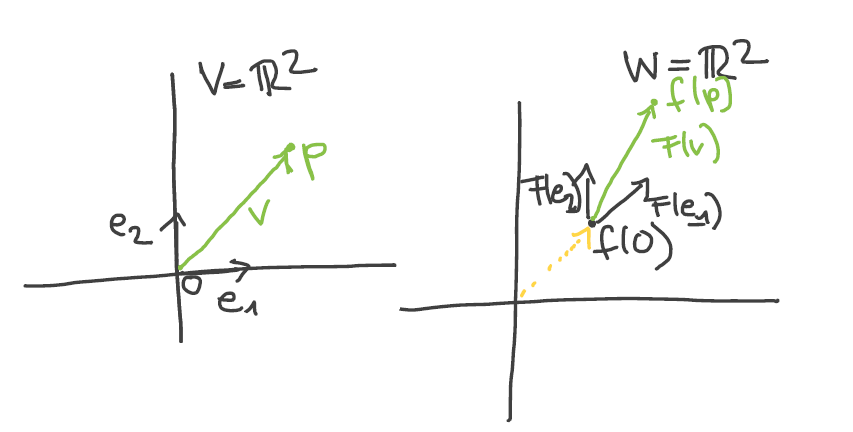
\includegraphics[width=0.7\linewidth]{figures/affine_abbildungen_vektorraeume}
    \label{fig:affine_abbildungen_vektorraeume}
\end{figure}
\begin{bemuebung*}
    Eine affine Abbildung \( f\maps X \to Y \) ist genau dann injektiv \bzw surjektiv \bzw bijektiv, wenn die zugehörige Abbildung \( F\maps T(X)\to T(Y) \).
\end{bemuebung*}
\begin{definition*}
    Wir nennen eine bijektive affine Abbildung \( f\maps X \to Y \) eine Affinität.
\end{definition*}
\section*{Affine Unterräume}
\begin{beispiel*}[\( \reals^2 \) als Vektorraum.]
    Untervektorräume von \( \reals^2 \) sind \( \emptyset \), \( \zeroset \), \( \reals^2 \) und Geraden durch \( 0 \).
    \begin{figure}[H]
        \centering
        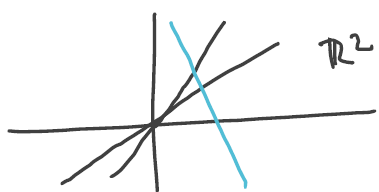
\includegraphics[width=0.4\linewidth]{figures/untervektorraeume_r2}
        \label{fig:untervektorraeume_r2}
    \end{figure}
    Betrachte nun \( \reals^2 \) als affinen Raum.
    \begin{figure}[H]
        \centering
        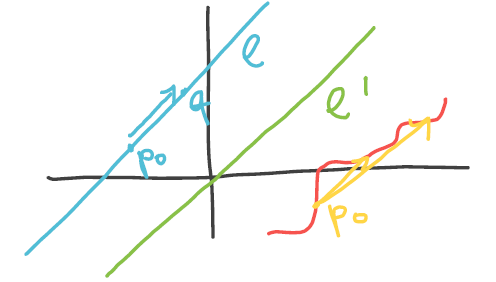
\includegraphics[width=0.5\linewidth]{figures/affine_unterraeume_r2}
        \label{fig:affine_unterraeume_r2}
    \end{figure}
    \begin{idee*}
        Wir wollen \( l \) und \( l' \) als affine Unterräume von \( \reals^2 \) definieren, da die Verschiebung von \( l, l' \) jeweils Untervektorräume von \( \reals^2 \) sind.
    \end{idee*}
\end{beispiel*}

\begin{definition*}
    Sei \( (X,T(X), \tau) \) in affiner Raum und \( Y\subseteq X \). Wenn es einen Punkt \( p_0 \in Y \) gibt, sodass
    \begin{align*}
        T(Y)\definedas \Set{\vv{p\circ q}\in T(X), q\in Y}
    \end{align*}
    ein Untervektorraum von \( T(X) \) ist, dann nennen wir \( Y \) einen affinen Unterraum von \( X \).
\end{definition*}
\begin{lemma}
    Sei \( Y\subseteq X \) ein affiner Unterraum eines affinen Raumes \( (X,T(X),\tau) \). Dann gilt
    \begin{align*}
        T(Y)=\Set{\vv{pq}\in T(X), q\in Y}
    \end{align*}
    für jedes beiliebigen Punkt \( p\in Y \).
\end{lemma}
\begin{proof}
    Sei \( p_0\in Y \) ein fester Punkt mit
    \begin{align*}
        T(Y)=\Set{\vv{p_0 q}\in T(X), q \in Y}
    \end{align*}
    Untervektorraum von \( T(X) \).
    Dann gilt für \( p \in Y \)
    \begin{align*}
        \Set{\vv{pq}|q\in Y}=\vv{pp_0}+\Set{\vv{p_0 q}| q\in Y}=\vertrelate{\vertni}{T(Y)}{\vv{p p_0}}+ T(Y)=T(Y),
    \end{align*}
    da \( \vv{p p_0}=-\vv{p_0 p}\in T(Y) \).
    
\end{proof}
\begin{definition*}
    Sei \( Y\subseteq X \) ein affiner Unterraum. Wir nennen \( \dim_K T(Y) \) die Dimension von \( Y \) und schreiben 
    \begin{align*}
        \dim Y=\dim_K T(Y).
    \end{align*}
\end{definition*}



% !TEX root = ./Vorlesungsmitschrift AGLA 2.tex  
\lecture{Fr 24.10. 10:15}{}
\section{Durchschnitt und Verbindung affiner Räume}
\begin{frage*}
    Sei \( X \) ein affiner Raum, \(    Y_1, Y_2 \) affine Unterräume von \( X \). Sind \( Y_1\cap Y_2, Y_1\cup Y_2 \) auch affine Unterräume von \( X \)?
    \begin{figure}[H]
        \centering
        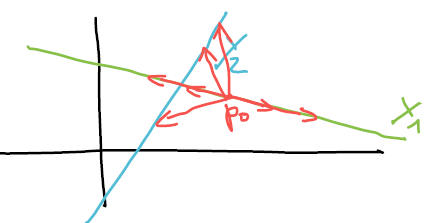
\includegraphics[width=0.5\linewidth]{figures/verbindung_affine_raeume}
        \caption*{\( X=\reals^2 \)}
        \label{fig:verbindung_affine_raeume}
    \end{figure}
\end{frage*}
\begin{lemma}\label{schnittraum:translationen}
    Sei \( X \) ein affiner Raum, \( Y_i \), \( i\in I \), eine Familie von affinen Unterräumen von \( X \).

    Dann ist \( Y\definedas \bigcap_{i\in I} Y_i \) ein affiner Unterraum von \( X \).

    Wenn \( Y\neq \emptyset \), dann gilt
    \begin{align*}
        T(Y)=\bigcap_{i\in I}T(Y_i).
    \end{align*}
\end{lemma}
\begin{proof}
    Falls \( Y=\emptyset \): \checkmark

    Wir nehmen also an \( Y\neq \emptyset \).
    Sei \( p_0\in Y \).
    Dann gilt:
    \begin{align*}
        T(Y)\begin{aligned}[t] 
            &=\Set{\underrelate{\textcolor{Goldenrod}\vertni}{\textcolor{Goldenrod}{T(X)}}{\vv{p_0 q}},q\in \bigcap_{i\in I}Y_i}\\
            &=\bigcap_{i\in I}\textcolor{LimeGreen}{\underbrace{\Set{\vv{p_0 q}, q\in Y_i}}_{=T(Y_i)}}\\
            &=\bigcap_{i\in I}T(\explain[big]{\text{Untervektorräume von \( T(X) \)}}{Y_i}).
        \end{aligned}
    \end{align*}
    Also ist \( T(Y) \) ein Untervektorraum von \( T(X) \) und \( T(Y)=\bigcap_{i\in I}T(Y_i) \).
\end{proof}
\begin{bemerkung*}
    In obiger Notation ist \( \bigcup_{i\in I}Y_i \) im Allgemeinen kein affiner Unterraum von \( X \).
\end{bemerkung*}
\begin{frage*}
    Finde den \enquote{kleinsten} affinen Unterraum von \( X \), der \( \bigcup_{i\in I}Y_i \) enthält! (\zb \( X\supseteq \bigcup_{i\in I} Y_i\), aber \( X \) ist im Allgemeinen nicht \enquote{minimal}).
\end{frage*}
\begin{definition*}
    Sei \( X \) ein affiner Raum, \( Y_i \), \( i\in I \) affine Unterräume von \( X \). Wir nennen
    \begin{align*}
        \bigcap_{\mathclap{\substack{Y\subseteq X \text{ aff.\ Unterraum}\\
         \bigcup_{i\in I}Y_i\subseteq Y}}}Y
    \end{align*}
    den \emph{Verbindungsraum} der affinen Unterräume \( Y_i \), \( i\in I \). Schreibe \( \bigvee_{i\in I}Y_i \).
\end{definition*}
\begin{beispiel*}
    \begin{figure}[H]
        \centering
        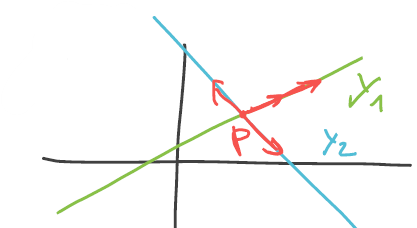
\includegraphics[width=0.5\linewidth]{figures/verbindungsraum_zwei_geraden}
        \caption*{\( X=\reals^2 \), \( Y_1\vee Y_2=X \), \textcolor{OrangeRed}{\( Y=Y_1\vee Y_2 \), \( T(Y)=T(Y_1)+T(Y_2) \)}.}
        \label{fig:verbindungsraum_zwei_geraden}
    \end{figure}
    
\end{beispiel*}

\begin{frage*}
    Wie kann man im Allgemeinen \( T(Y_1\vee Y_2) \) aus \( T(Y_1),T(Y_2) \) bestimmen?
\end{frage*}
\begin{lemma}\label{verbindungsraum:translationen}
    Sei \( X \) ein affiner Raum, \( Y_1,Y_2\neq\emptyset \) affine Unterräume von \( X \).
    \begin{eigenschaftenenumerate}
        \item \label{verbindungsraum:translationen:schnitt_nicht_leer}Sei \( Y_1\cap Y_2\neq \emptyset \).
        Dann gilt
        \begin{align*}
            T(Y_1\vee Y_2)=T(Y_1)+T(Y_2).
        \end{align*}
        
        \item \label{verbindungsraum:translationen:schnitt_leer}Sei \( Y_1\cap Y_2=\emptyset \), \( p_1\in Y_1, p_2\in Y_2\) und \( Y=p_1\vee p_2 \).
        
        Dann gilt:
        \begin{align*}
            T(Y_1\vee Y_2)=(T(Y_1)+T(Y_2))\oplus T(Y).
        \end{align*}
    \end{eigenschaftenenumerate}
\end{lemma}
\begin{proof}
    \begin{proofdescription}
        
        \item[\ref{verbindungsraum:translationen:schnitt_nicht_leer}]
        \begin{figure}[H]
            \centering
            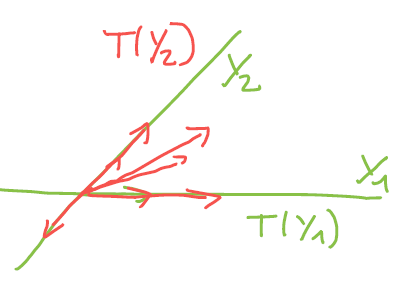
\includegraphics[width=0.5\linewidth]{figures/verbindungsraum_translationen_schnitt_nicht_leer}
            \label{fig:verbindungsraum_translationen_schnitt_nicht_leer}
        \end{figure}
         Sei \( p\in Y_1\cap Y_2 \). Dann gilt
         \begin{align*}
             T(Y_1)\cup T(Y_2)\begin{aligned}[t] 
                &=\Set{\vv{pq}|q\in Y_1\cup Y_2}\\
                &\subseteq T(Y_1\vee Y_2),
             \end{aligned}
         \end{align*}
         also \( T(Y_1)+T(Y_2)\subseteq T(Y_1\vee Y_2) \).

         Sei \( Y=\Set{\tau_t(p)|t\in T(Y_1)+T(Y_2)} \).
         Dann ist \( Y \) affiner Unterraum von \( X \) mit \( Y_1\cup Y_2\subseteq Y \), also \( Y_1\vee Y_2\subset Y \), also \( Y_1\vee Y_2\subseteq Y \). Also gilt
         \begin{align*}
             T(Y_1\vee Y_2)\subseteq T(Y)=T(Y_1)+T(Y_2).
         \end{align*}
         
         Also \( T(Y_1\vee Y_2)=T(Y_1)+T(Y_2) \).
         
         \item[\ref{verbindungsraum:translationen:schnitt_leer}]
         \( Y_1\cap Y_2=\emptyset \), \( p_1\in Y_1 \), \( p_2\in Y_2 \), \( Y=p_1\vee p_2 \).
         \begin{figure}[H]
             \centering
             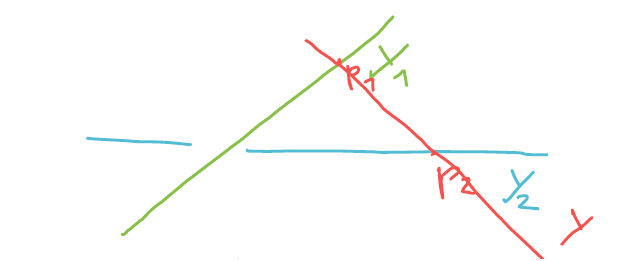
\includegraphics[width=0.5\linewidth]{figures/verbindungsraum_translationen_schnitt_leer}
             \label{fig:verbindungsraum_translationen_schnitt_leer}
         \end{figure}
         Schreibe \( Y_1\vee Y_2=Y_1\vee Y\vee Y_2 \) (verwende dazu \( Y\subseteq Y_1\vee Y_2 \)).
         Verwende \ref{verbindungsraum:translationen:schnitt_nicht_leer} und leite ab, dass gilt:
         \begin{align*}
             T(Y_1\vee Y \vee Y_2)\begin{aligned}[t] 
                 &=T(Y_1)+T(Y\vee Y_2)\\
                 &=T(Y_1)+T(Y)+T(Y_2)\\
                 &=(T(Y_1)+T(Y_2))\needed{\oplus} T(Y).
             \end{aligned}
         \end{align*}
         Es gilt 
         \begin{align*}
             T(Y)=\Set{\lambda\vv{p_1 p_2}| \lambda\in K}.
         \end{align*}
         Wir wollen zeigen
         \begin{align*}
             (T(Y_1)+T(Y_2))\cap T(Y)=\zeroset.
         \end{align*}
         Es genügt zu zeigen
         \begin{align*}
             \vv{p_1 p_2}\notin T(Y_1)+T(Y_2).
         \end{align*}
         Gegenannahme:
         \begin{align*}
             \vv{p_1 p_2}=\underrelate{\vertni}{T(Y_1)}{\vv{p_1 y_1}}+\underrelate{\vertni}{T(Y_2)}{\vv{q_2 p_2}}
         \end{align*}
         mit \( q_1\in Y_1 \), \( q_2\in Y_2 \).
         \begin{figure}[H]
             \centering
             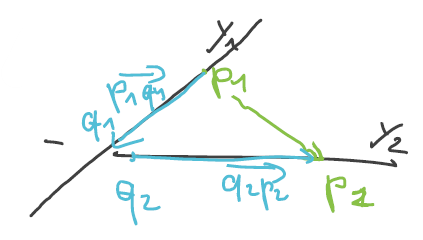
\includegraphics[width=0.5\linewidth]{figures/verbindungsraum_translationen_schnitt_leer_verbindungslinie_nicht_in_translationen}
             \label{fig:verbindungsraum_translationen_schnitt_leer_verbindungslinie_nicht_in_translationen}
         \end{figure}
         Dann gilt
         \begin{align*}
             \vv{q_1 q_2}=\vv{q_1 p_1}+\vv{p_1 p_2}+\vv{p_2 q_2}=0,
         \end{align*}
         also \( q_1=q_2 \) und \( Y_1\cap Y_2\neq \emptyset \) \contra.
    \end{proofdescription}
\end{proof}
Als nächstes: \( \dim(Y_1\vee Y_2) \) ist durch \( \dim_K T(Y_1\vee Y_2) \) gegeben, also sollten wir aus \thref{verbindungsraum:translationen} für \( Y_1\vee Y_2 \) ableiten können.
\begin{lemma}\label{verbindungsraum:dimension}
    Sei \( X \) ein affiner Raum, \( Y_1, Y_2\neq \emptyset \) affine Unterräume von \( X \).
    \begin{eigenschaftenenumerate}
        \item\label{verbindungsraum:dimension:schnitt_nicht_leer} Sei \( Y_1\cap Y_2\neq \emptyset \).
         Dann gilt \( \dim(Y_1\vee Y_2)=\dim(Y_1)+\dim(Y_2)-\dim(Y_1\cap Y_2) \).
        \item\label{verbindungsraum:dimension:schnitt_leer} Sei \( Y_1\cap Y_2=\emptyset \).
        Dann gilt
        \begin{align*}
            \dim(Y_1\vee Y_2)=\dim(Y_1)+\dim(Y_2)-\dim(T(Y_1)\cap T(Y_2))+1.
        \end{align*}
    \end{eigenschaftenenumerate}
    
\end{lemma}
\begin{proof}
    \begin{proofdescription}
        
        \item[\ref{verbindungsraum:dimension:schnitt_nicht_leer}] Aus \thref{verbindungsraum:translationen} folgt
        \begin{align*}
            T(Y_1\vee Y_2)=T(Y_1)+T(Y_2),
        \end{align*}
        aus der Dimensionsformel für Untervektorräume folgt
        \begin{equation*}
            \dim (Y_1\vee Y_2)\begin{aligned}[t] 
                &=\dim T(Y_1\vee Y_2)\\
                &=\dim(Y_1)+\dim T(Y_2)-\dim(T(Y_1)\cap T(Y_2))\\
                &\explain{\text{\thref{schnittraum:translationen}}}{=}\dim T(Y_1)+\dim T(Y_2)-\dim T(Y_1\cap Y_2)\\
                &=\dim Y_1+\dim Y_2-\dim Y_1\cap Y_2.
            \end{aligned}
        \end{equation*}
        
        \item[\ref{verbindungsraum:dimension:schnitt_leer}] \( Y_1\cap Y_2 \), \( p_1\in Y_1 \), \( p_2\in Y_2 \), \( Y=p_1\vee p_2 \).
        
        Dann ist
        \begin{align*}
            \dim Y=\dim T(Y)=1.
        \end{align*}
        Wir erhalten
        \begin{align*}
            \dim (Y_1\vee Y_2)\begin{aligned}[t] 
                &=\dim T(Y_1\vee Y_2)\\
                &\explain{\text{\thref{verbindungsraum:translationen}}}{=}\dim((T(Y_1)+T(Y_2))\oplus T(Y))\\
                &=\dim(T(Y_1)+T(Y_2))+\equalto{1}\dim T(Y)\\
                &=\dim T(Y_1)+\dim T(Y_2)- \dim (T(Y_1)\cap T(Y_2))+1\\
                &=\dim Y_1+\dim Y_2 -\dim(T(Y_1)\cap T(Y_2))+1
            \end{aligned}
        \end{align*}
    \end{proofdescription}
\end{proof}
\begin{beispiel*}[\( X=\reals^3 \)]
    \begin{figure}[H]
        \centering
        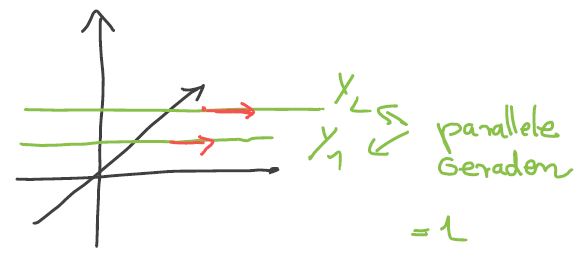
\includegraphics[width=0.5\linewidth]{figures/verbindungsraum_parallele_geraden}
        \label{fig:verbindungsraum_parallele_geraden}
    \end{figure}
    \begin{align*}
        \dim (Y_1\vee Y_2)=1+1-\underbrace{\dim(T(Y_1)\cap T(Y_2))}_{=1}+1=2
    \end{align*}
    \begin{figure}[H]
        \centering
        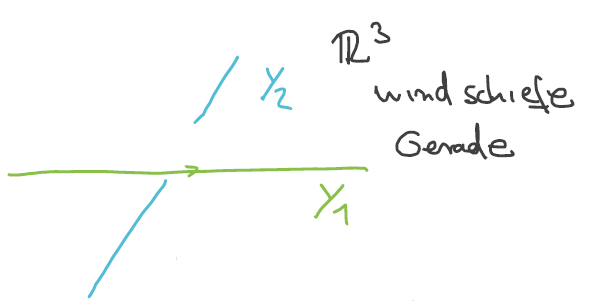
\includegraphics[width=0.6\linewidth]{figures/verbindungsraum_windschiefe_geraden}
        \label{fig:verbindungsraum_windschiefe_geraden}
    \end{figure}
    \begin{align*}
        \dim (Y_1\vee Y_2)1+1-0+1=3
    \end{align*}
    und \( Y_1\vee Y_2=X \).
    
\end{beispiel*}
\section{Parallelprojektionen}
\begin{wiederholung*}[Projektionen aus der \agla{1}]
    \begin{beispiel*}
        \begin{figure}[H]
            \centering
            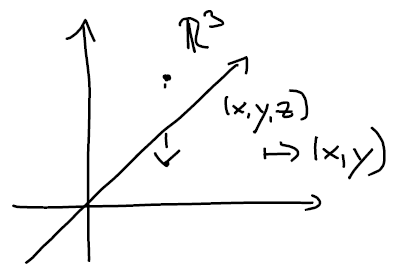
\includegraphics[width=0.5\linewidth]{figures/r_3_projektion}
            \label{fig:r_3_projektion}
        \end{figure}
        
    \end{beispiel*}
    Sei \( V \) ein \( K \)-Vektorraum, \( W, W_1\subset V \) \( K \)-Untervektorräume mit \( V=W\oplus W_1 \).
    Schreibe \( v\in V \) in der Form \( v=w+w_1 \) und mit \( w\in W \), \( w_1\in W_1 \). Definiere
    \begin{align*}
        P_W\maps \begin{aligned}[t] 
            V&\to W_1\\
            \equalto{w+w_1}{v}&\mapsto w_1.
        \end{aligned}
    \end{align*}
    Ein paar Eigenschaften von \( P_W \):
    \begin{itemize}
        \item \( P_W\maps V \to W_1 \) ist eine lineare Abbildung,
        \item \( \Ker P_W=W \),
        \item \( \evaluateat{P_W}{W_1}=\Id_{W_1} \).
    \end{itemize}
    Als Nächstes:
    Wir schränken \( P_W \) ein auf einen Untervektorraum \( W_0 \) von \( V \).
    \begin{figure}[H]
        \centering
        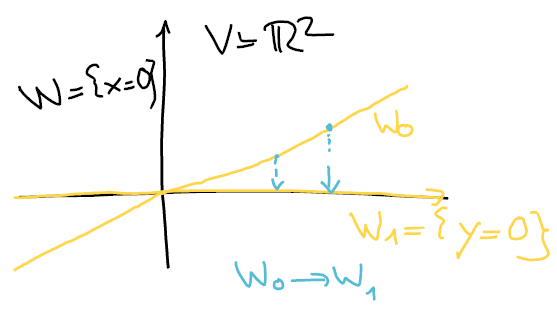
\includegraphics[width=0.5\linewidth]{figures/projektion_einschraenkung_auf_w_0}
        \label{fig:projektion_einschraenkung_auf_w_0}
    \end{figure}
    \begin{lemma}\label{projektion_isomorph}
        Sei \( V \) ein \( K \)-Vektorraum, \( W,W_0, W_1\subseteq V \) Untervektorräume mit \( V=W\oplus W_0=W\oplus W_1 \).

        Dann ist \( \evaluateat{P_W}{W_0}\maps W_0\to W_1 \) ein Isomorphismus (Notation wie oben).
    \end{lemma}
    \begin{proof}
        Es gilt \( \dim W_0=\dim W_1 \) und es genügt zu zeigen, dass \( \evaluateat{P_W}{W_0} \) injektiv ist.

        Sei \( \evaluateat{P_W}{w_0}=w_1 \) für \( w_0\in W_0 \), \( w_1\in W_1 \). Dann ist \( w_0=w+w_1 \) mit \( w\in W \), \( w_1\in W_1 \), also
        \begin{align*}
            w_1=\underrelate{\textcolor{LimeGreen}{\vertni}}{\textcolor{LimeGreen}{W_0}}{w_0}-\underrelate{\textcolor{LimeGreen}{\vertni}}{\textcolor{LimeGreen}{W}}{w}\in W_0\oplus W,
        \end{align*}
        und diese Zerlegung ist eindeutig.
        
    \end{proof}
    
\end{wiederholung*}
\subsection*{Parallelprojektionen für affine Räume}
Sei \( X \) ein affiner Raum (über einem Körper \( K \)), \( Y_1\subseteq X \) ein affiner Unterraum
\begin{beispiel*}
    \begin{figure}[H]
        \centering
        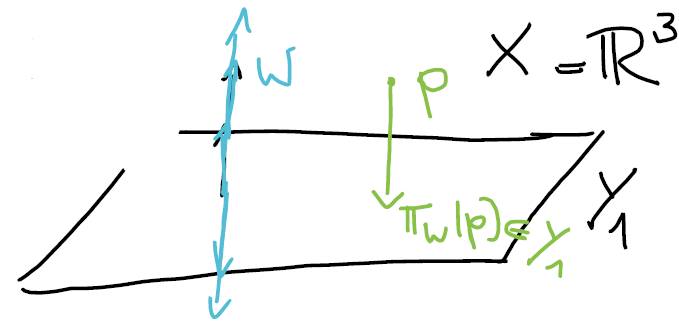
\includegraphics[width=0.5\linewidth]{figures/affine_parallelprojektion_r_3}
        \label{fig:affine_parallelprojektion_r_3}
    \end{figure}
    
\end{beispiel*}
Sei \( W\subseteq T(X) \) ein Untervektorraum mit \( T(X)=T(Y_1)\oplus W \).
\begin{ziel*}
    Definiere eine Projektionsabbildung
    \begin{align*}
        \pi_W\maps X\to Y_1
    \end{align*}
    \enquote{längs \( W \)}.
\end{ziel*}
Für \( p\in X \) definiere
\begin{align*}
    W(p)\definedas\Set{x\in X| \vv{px}\in W}
\end{align*}
\begin{lemma}
    Notation wie oben.
    Für \( p\in X \) gilt
    \begin{align*}
        \anzahl(Y_1\cap W(p))=1.
    \end{align*}
\end{lemma}
\begin{proof}
    Wir berechnen
    \begin{align*}
        \dim(Y_1\cap W(p)).
    \end{align*}
    Sei \( x=\dim X \), verwende \thref{verbindungsraum:dimension}~\ref{verbindungsraum:dimension:schnitt_leer}.
    Falls \( Y_1\cap W(p)=\emptyset \), dann
    \begin{align*}
        \dim(Y_1\vee W(p))\begin{aligned}[t] 
            &=\dim Y_1+\dim W(p)-\dim(\underbrace{T(Y_1)\cap W}_{\textcolor{LimeGreen}{=\zeroset}})+1\\
            &=\dim T(Y_1)+\dim W+1
        \end{aligned}
    \end{align*}
    \contra zu \( Y_1\vee W(p)\subseteq X \), also ist \( Y_1\cap W(p)\neq \zeroset \), und nach \thref{verbindungsraum:dimension}~\ref{verbindungsraum:dimension:schnitt_nicht_leer} gilt Folgendes:
    \begin{align*}
        \equalto{n}{\underbrace{\dim (Y_1\vee W(p))}}\begin{aligned}[t] 
            &=\dim Y_1+\dim W(p)-\dim(Y_1\cap W(p))\\
            &=n-\dim(Y_1\cap W(p))
        \end{aligned}
    \end{align*}
    und nach \thref{schnittraum:translationen}
    \begin{align*}
        \dim Y_1\vee W(p)\begin{aligned}[t] 
            &=\dim(T(Y_1)+W)\\
            &=n,
        \end{aligned}
    \end{align*}
    also \( \dim(Y_1\cap W(p))=0 \).
    
\end{proof}
Wir definieren die Projektion längs \( W \)
\begin{align*}
    \pi_W\maps \underrelate{\subseteq}{Y_0}{X}\to Y_1,\logicspace p\mapsto W(p)\cap Y_1.
\end{align*}
\begin{satz}
    Sei \( X \) ein affiner Raum, \( Y_1,Y_0\subseteq X \) affine Unterräume, \( W\subseteq T(X) \) ein Untervektorraum mit 
    \begin{align*}
        T(X)=W\oplus T(Y_0)=W\oplus T(Y_1).
    \end{align*}
    Dann ist \( \pi_W\maps X\to Y_1 \) eine surjektive affine Abbildung und \( \evaluateat{\pi_w}{Y_0}\maps Y_0\to Y_1 \) eine Affinität.
\end{satz}
\begin{proof}
    Seien \( p,q\in X \).
    \begin{figure}[H]
        \centering
        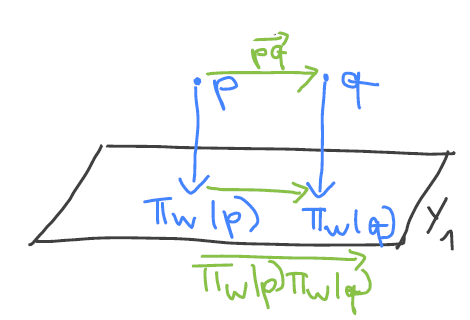
\includegraphics[width=0.5\linewidth]{figures/affine_projektion_ist_affin}
        \label{fig:affine_projektion_ist_affin}
    \end{figure}
    Dann gilt
    \begin{align*}
        \vv{pq}\begin{aligned}[t] 
            &=\vv{p\pi_W(p)}+\vv{\pi_W(p)\pi_W(q)}+\vv{\pi_W(q)q}+\vv{\pi_W(q)q}\\
            &=\underbrace{\vv{p\pi_W(p)}+\vv{\pi_W(q)q}}_{\textcolor{Cyan}{\in W}}+\underbrace{\vv{\pi_W(p)\pi_W(q)}}_{\textcolor{Cyan}{\in T(Y_1)}},
        \end{aligned}
    \end{align*}
    also \( \vv{\pi_W(p)\pi_W(q)}=P_W(\vv{pq}) \).

    \( P_W \) ist surjektiv, also ist \( \pi_W \) eine surjektive affine Abbildung.

    Der zweite Teil folgt aus \thref{projektion_isomorph}.
\end{proof}
% !TEX root = ./Vorlesungsmitschrift AGLA 2.tex  
\lecture{Di 28.04. 10:15}{}
\section{Affine Koordinaten}
Koordinaten in einem \( K \)-Vektorraum \( V \). Sei \( \dim V=n \) und \( v_1,\dotsc , v_n \) eine Basis von \( V \). Dann ist die Abbildung
\begin{align*}
    \phi\maps  \begin{aligned}[t]
        K^n&\to V\\
        (x_1,\dotsc,x_n)&\mapsto \sum\limits_{i=1}^{n}x_i v_i
    \end{aligned}
\end{align*}
ein Isomorphismus von \( K \)-Vektorräumen. Jeder Punkt \( \underrelate{\ni}{V}{v}=\sum_{i=1}^{n}x_i v_i \) ist eindeutig bestimmt durch seine \enquote{Koordinaten}
\begin{align*}
    \inf{\phi}(v)=(x_1,\dotsc,x_n)\in K^n.
\end{align*}
\begin{frage*}
    Sei \( X \) ein affiner Raum über einem Körper \( K \). Können wir auch hier die Lage eines Punkte \( p\in X \) durch Angabe von \enquote{Koordinaten} bezüglich einer \enquote{Basis} beschreibe?
    \begin{figure}[H]
        \centering
        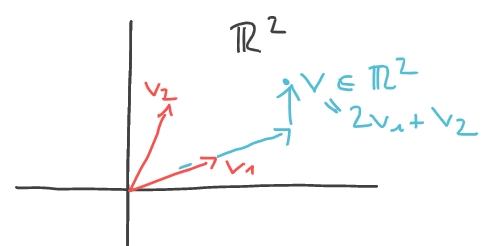
\includegraphics[width=0.5\linewidth]{figures/affine_koordinaten_r_2_hoffnung}
        \label{fig:affine_koordinaten_r_2_hoffnung}
    \end{figure}
    
\end{frage*}
\begin{bspidee*}
    \( X=\reals^2 \) als affiner Raum und Punkte \( p_1,p_2\in X \), sodass \( \vv{p_0p_1} \), \( \vv{p_0p_2} \) eine Basis ist für \( T(X) \). Dann können wir einen Punkt \( p\in X \) beschreiben durch
    \begin{align*}
        p \begin{aligned}[t]
            &=\tau_{\vv{p_0p}}(p_0)\\
            &=\tau_{\lambda\vv{p_0p_1}+\mu\vv{p_0p_2}}(p_0),
        \end{aligned}
    \end{align*}
    falls \( \vv{p_0p}=\lambda\vv{p_0p_1}+\mu\vv{p_0p_2} \) mit \( \lambda,\mu\in \reals \).

    \begin{figure}[H]
        \centering
        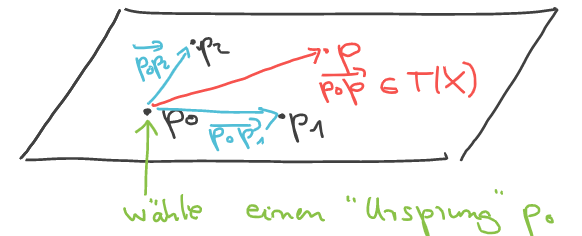
\includegraphics[width=0.5\linewidth]{figures/ursprungswahl}
        \label{fig:ursprungswahl}
    \end{figure}
    
    Wir erhalten eine Abbildung 
    \begin{align*}
        \phi\maps \begin{aligned}[t]
            \reals^2&\to X\\
            (\lambda,\mu)&\mapsto \tau_{\lambda\vv{p_0 p_1}+\mu\vv{p_0 p_2}}(p_0),
        \end{aligned}
    \end{align*}
    die eine Affinität ist.
\end{bspidee*}
Wir formalisieren diese Konzepte für allgemeine affine Räume.
\begin{definition*}
    Sei \( X \) ein affiner Raum und \( p_0,\dotsc, p_n\in X \). Wir nennen \( (p_0,\dotsc,p_n) \) \emph{affin unabhängig} \bzw eine \emph{affine Basis}, wenn die Vektoren \( (\vv{p_0p_1},\dotsc, \vv{p_0p_n}) \) in \( T(x) \) \emph{linear unabhängig sind} \bzw \emph{eine Basis bilden}.
\end{definition*}
\begin{beispiele*}
    \begin{enumerate}
        \item In \( X=\reals^n \) ist \( (0,e_1,\dotsc, e_n) \) eine affine Basis.
        \item \( X=\reals^n \) als affiner Raum, \( v_1,\dotsc, v_k\in \reals^n \) linear unabhängig, \( v_0=0 \). Dann ist das Tupel \( (v_0,v_1,\dotsc,v_k) \) affin unabhängig.
        \begin{frage*}
            Kann man hier \( v_0\in \reals^n \) beliebig nehmen?
        \end{frage*}
        \item \( X=\reals^2 \) als affiner Raum. Dann gilt, dass für \( v,w\in \reals^2 \) das Tupel \( (v,w) \) affin unabhängig ist \gdw \( v\neq w \).
        \item \( X \) affiner Raum, \( p_0\in X \), \( (t_1,\dotsc,t_n) \) Basis von \( T(X) \). Dann ist
        \begin{align*}
            (p_0,\tau_{t_1}(p_0),\dotsc, \tau_{t_n}(p_0))
        \end{align*}
        eine affine Basis von \( X \).
    \end{enumerate}
    
\end{beispiele*}
\begin{lemma}
    Sei \( X \) ein affiner Raum, \( p_0,\dotsc, p_n\in X \) und \( (p_0,\dotsc, p_n) \) affin unabhängig. Sei \( \sigma\in S_{n+1} \) eine Permutation von \( \Set{0,\dotsc,n} \). Dann ist
    \begin{align*}
        (p_{\sigma(0)},p_{\sigma(1)},\dotsc,p_{\sigma(n)})
    \end{align*}
    affin unabhängig.
\end{lemma}
\begin{proof}
    Wir wollen zeigen, dass unter den Annahmen des Lemmas, die Vektoren
    \begin{align*}
        \vv{p_{\sigma(0)}p_{\sigma(1)}},\dotsc,\vv{p_{\sigma(0)p_{\sigma(n)}}}\in T(X)
    \end{align*}
    linear unabhängig sind.

    Sei \( \sigma(0)=i\in \Set{0,\dotsc,n} \).

    Dann müssen wir also zeigen, dass die Vektoren
    \begin{align*}
        \vv{p_i p_0},\vv{p_i p_1},\dotsc, \vv{p_i p_{i-1}},\vv{p_i p_{i+1}},\dotsc,\vv{p_i p_n}
    \end{align*}
    linear unabhängig sind.

    Seien \( \lambda_0,\dotsc, \lambda_{i-1},\lambda_{i+1},\dotsc,\lambda_n\in K \) mit
    \begin{align*}
        \lambda_0 \vv{p_i p_0}+\lambda_1\vv{p_i p_1}+\dotsb+\lambda_{i-1}\vv{p_i p_{i-1}}+\lambda_{i+1}\vv{p_i p_{i+1}}+\dotsb+\lambda_n\vv{p_i p_n}=0.
    \end{align*}
    Schreibe
    \begin{align*}
        \vv{p_i p_j}=\vv{p_i p_0}+\vv{p_0 p_j}=\textcolor{Goldenrod}{\vv{p_0 p_j}}-\textcolor{LimeGreen}{\vv{p_0 p_i}}.
    \end{align*}
    Wir erhalten
    \begin{align*}
        \begin{aligned}[t]
            \textcolor{Goldenrod}{\lambda_1\vv{p_0 p_1}+\dotsb+\lambda_{i-1} \vv{p_0 p_{i-1}}+\lambda_{i+1} \vv{p_0 p_{i+1}}+\dotsb+\lambda_n \vv{p_0 p_n}}\\
            -\textcolor{LimeGreen}{(\lambda_0+\dotsb+\lambda_{i-1}+\lambda_{i+1}+\dotsb+\lambda_n)\vv{p_0 p_i}}=0
        \end{aligned}
    \end{align*}
    Aus der linearen Unabhängigkeit von \( \vv{p_0 p_1},\dotsc, \vv{p_0 p_n} \) folgt
    \begin{align*}
        \lambda_1=\dotsb=\lambda_{i-1}=\lambda_{i+1}=\lambda_n=0
    \end{align*}
    und
    \begin{align*}
            \explain{\lambda_0=0}+\underbrace{\lambda_1+\dotsb+\lambda_{i-1}+\lambda_{i+1}+\dotsb+\lambda_n}_{=0}=0
    \end{align*}
\end{proof}
\subsection*{Affine Basen und affine Abbildungen}
Aus der AGLA \Romannum{1}:\\
Seien \( V,W \) \( K \)-Vektorräume, \( v_1,\dotsc, v_n \in V \) eine Basis von \( V \) und \( w_1,\dotsc, w_n \in W\). Dann gibt es genau eine \( K \)-lineare Abbildung \( \phi\maps V\to W \) mit
\begin{align*}
    \phi(v_i)=w_i,\quad 1\leq i \leq n.
\end{align*}
\begin{figure}[H]
    \centering
    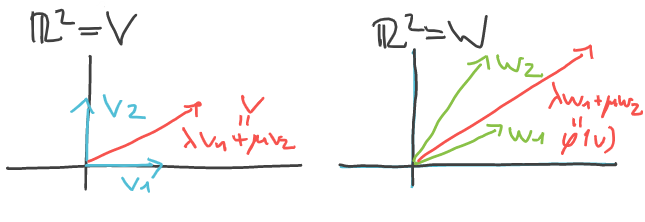
\includegraphics[width=0.7\linewidth]{figures/bilder_der_basen_bestimmt_abbildung_r_2}
    \label{fig:bilder_der_basen_bestimmt_abbildung_r_2}
\end{figure}
\begin{frage*}
    Inwiefern sind affine Abbildungen zwischen affinen Räumen durch die Bilder einer affinen Basis bestimmt?
\end{frage*}
\begin{satz}\label{bilder_der_basen_bestimmen_affine_abbildung}
    Seien \( X,Y \) affine Räume, \( (p_0,\dotsc,p_n) \) eine affine Basis von \( X \) und \( q_0,\dotsc, q_n\in Y \). Dann gibt es genau eine affine Abbildung \( f\maps X\to Y \) mit
    \begin{align*}
        f(p_i)=q_i,\quad 0\leq i\leq n.
    \end{align*}
    Die Abbildung \( f \) ist \emph{injektiv} \bzw \emph{eine Affinität} \gdw das Tupel \( (q_0,\dotsc, q_n) \) \emph{affin unabhängig} \bzw \emph{eine affine Basis} von \( Y \) ist.
\end{satz}
\begin{proof}
    Eine affine Abbildung \( f\maps X\to Y \) ist gegeben durch \( f(p_0) \) für ein \( p_0\in X \) und eine lineare Abbildung
    \begin{align*}
        F\maps \begin{aligned}[t]
            T(X)&\to T(Y)\\
            \vv{pq}&\mapsto \vv{f(p)f(q)}.
        \end{aligned}
    \end{align*}
    Wir definieren \( F \) durch
    \begin{align*}
        F(\vv{p_0 p_i})=\vv{q_0 q_i}\quad 1\leq i \leq n. \tag{*}\label{bilder_der_basen_bestimmt_affine_abbildung:beweis:k_lineare_abbildung}
    \end{align*}
    \( \vv{p_0 p_1}, \dotsc, \vv{p_0 p_n} \) ist eine Basis von \( T(X) \), also gibt es genau ein lineare Abbildung
    \begin{align*}
        F\maps T(X)\to T(Y)
    \end{align*}
    mit \eqref{bilder_der_basen_bestimmt_affine_abbildung:beweis:k_lineare_abbildung}. Es gilt dann
    \begin{align*}
        f(p_i)\begin{aligned}[t]
            &=\tau_{\vv{f(p_0) f(p_i)}} f(p_0)\\
            &=\tau_{F(\vv{p_0 p_i})} f(p_0)\\
            &=\tau_{\vv{q_0 q_i}} q_0 =q_i \quad 1\leq i \leq n.
        \end{aligned}
    \end{align*}
    \( f \) ist injektiv \gdw \( F \) injektiv ist. \( F \) ist injektiv \gdw \( \vv{q_0 q_1}, \dotsc, \vv{q_0 q_n} \) linear unabhängig sind.

    \tto \( f \) ist eine Affinität \gdw \( F \) bijektiv ist. \( F \) ist bijektiv \gdw \( \vv{q_0 q_1}, \dotsc, \vv{q_0 q_n} \) eine Basis von \( T(Y) \) ist.

\end{proof}
\subsection*{Affine Koordinatensysteme}
Sei \( X \) ein affiner Raum über einem Körper \( K \), \( (p_0,p_1,\dotsc, p_n) \) eine affine Basis von \( X \).

Nach \thref{bilder_der_basen_bestimmen_affine_abbildung} gibt es genau eine Affinität
\begin{align*}
    \phi\maps K^n\to X
\end{align*}
mit \( \phi(0)=p_0, \phi(e_1)=p_1,\dotsc, \phi(e_n)=p_n \) und zugehörige lineare Abbildung \( \Phi\maps K^n \to T(X) \).

Einen Punkt \( p\in X \) können wir dann beschreiben durch
\begin{align*}
    p=\tau_{\vv{p_0 p}}(p_0).
\end{align*}
Sei \( \vv{p_0 p}=\lambda_1 \vv{p_0 p_1}+\dotsb +\lambda_n \vv{p_0 p_n} \) mit \( \lambda_i\in K \), \( 1\leq i \leq n \).

Dann ist
\begin{align*}
    p \begin{aligned}[t]
        &=\tau_{\lambda_1\vv{p_0 p_1}+\dotsb +\lambda_n\vv{p_0 p_n}}(p_0)\\
        &=\tau_{\lambda_1 \Phi(e_1)+\dotsb+\lambda_n \Phi(e_n)}(p_0)\\
        &=\tau_{\Phi(\lambda_1 e_1+\dotsb+\lambda_n e_n)}(p_0),
    \end{aligned}
\end{align*}
oder \( p=\phi((\lambda_1,\dotsc,\lambda_n)) \).

\begin{definition*}
    Sei \( X \) ein affiner Raum über einem Körper \( K \). Wir nennen eine Affinität \( \phi\maps K^n\to X \) ein affines Koordinatensystem in \( X \). Seu \( p_0=\phi(0),p_1=\phi(e_1),\dotsc, p_n=\phi(e_n) \). Dann ist \( (p_0,\dotsc,p_n) \) eine affine Basis von \( X \).

    Für \( p\in X \) nennen wir
    \begin{align*}
        \inv{\phi}(p)=(x_1,\dotsc,x_n)\in K^n
    \end{align*}
    den Koordinatenvektor von \( p \) bezüglich der affinen Basis \( (p_0,\dotsc,p_n) \) und \( (x_1,\dotsc, x_n) \) die Koordinaten von \( p \) bezüglich \( (p_0,\dotsc, p_n) \).
    \begin{figure}[H]
        \centering
        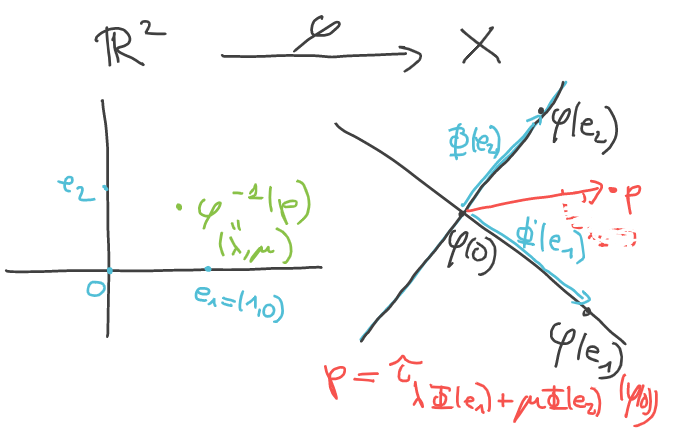
\includegraphics[width=0.7\linewidth]{figures/affine_koordinatenabbildung_r_2}
        \label{fig:affine_koordinatenabbildung_r_2}
    \end{figure}
\end{definition*}
\section{Das Teilverhältnis}
\begin{idee*}
    Seien 3 Punkte \( p_0,p_1,p \) auf einer Gerade \( l \) (\zb im \( \reals^3 \)) gegeben, \( p_0\neq p_1 \).
    \begin{figure}[H]
        \centering
        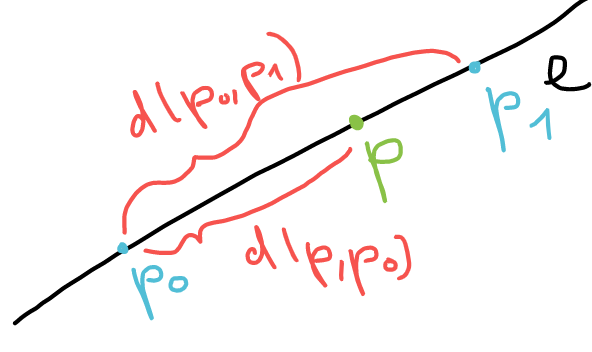
\includegraphics[width=0.5\linewidth]{figures/gerade_teilverhaeltnis}
        \caption*{}
        \label{fig:gerade_teilverhaeltnis}
    \end{figure}
    Sei \( \lambda=\frac{d(p,p_0)}{d(p_1,p_0)} \), mit \( d \) dem euklidischen Abstand, dann können wir die Lage von \( p \) auf \( l \) durch \( \lambda \) (und der Information, ob \( p \) \enquote{rechts oder links} von \( p \) liegt) bestimmen.
\end{idee*}
\begin{definition*}
    Sei \( X \) ein affiner Raum über \( K \), \( Y\subseteq X \) eine affine Gerade, \( p_0,p_1,p\in Y \) und \( p_0\neq p_1 \). Dann nennen wir das eindeutig bestimmte Element \( \lambda\in K \) mit \( \vv{p_0 p}=\lambda \vv{p_0 p_1} \) das Teilverhältnis von \( p_0,p_1,p \). Schreibe \( \lambda=\teilverhaeltnis(p_0,p_1,p) \). In \( \characteristic(K)\neq 2 \) nennen wir \( p \) Mittelpunkt von \( p_0,p_2 \) wenn \( \teilverhaeltnis(p_0,p_1,p)=\frac{1}{2} \).
\end{definition*}
\begin{bemerkungen*}
    \begin{enumerate}
        \item Es gilt \( T(Y)=K\vv{p_0p_1} \). Damit ist \( \lambda \) wohldefiniert und existiert.
        \item \( p_0,p_1 \) ist eine affine Basis von \( Y \). Damit existiert ein Koordinatensystem
        \begin{align*}
            \phi\maps K\to Y,\logicspace \begin{aligned}[t]
                \phi(0)&=p_0\\
                \phi(1)&=p_1
            \end{aligned}
        \end{align*}
        und es gilt \( \teilverhaeltnis(p_0,p_1,p)=\inv{\phi(p)} \).
    \end{enumerate}
    
\end{bemerkungen*}
\begin{frage*}
    Wie verhält sich das Teilverhältnis unter affinen Abbildungen?
    \begin{figure}[H]
        \centering
        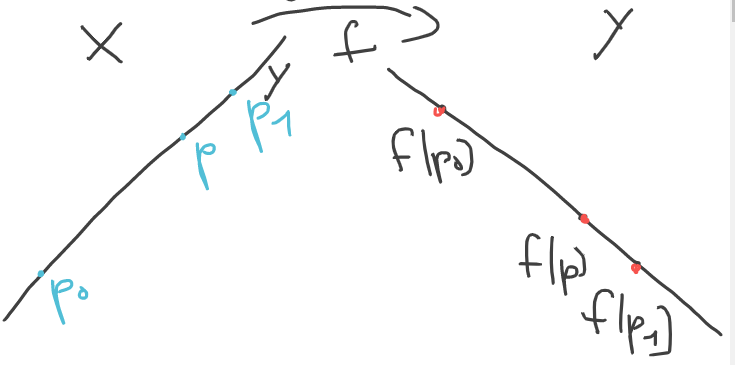
\includegraphics[width=0.7\linewidth]{figures/affine_abbildungen_wirkung_auf_teilverhaeltnis}
        \label{fig:affine_abbildungen_wirkung_auf_teilverhaeltnis}
    \end{figure}
    
\end{frage*}

\begin{lemma}\label{teilverhaeltnis_invariant_unter_affinen_abbildungen}
    Seien \( X,Y \) affine Räume und \( f\maps X\to Y \) eine affine Abbildung, seien \( p_0,p1,p \) Punkte in \( X \), die auf einer Geraden liegen und \( f(p_0)\neq f(p_1) \). Dann gilt
    \begin{align*}
        \teilverhaeltnis(f(p_0),f(p_1),f(p))=\teilverhaeltnis(p_0,p_1,p).
    \end{align*}
\end{lemma}
\begin{proof}
    Sei \( \lambda=\teilverhaeltnis(p_0,p_1,p) \), also \( \vv{p_0 p}=\lambda\vv{p_0 p_1} \). Si \( F\maps T(X)\to T(Y) \) die zu \( f \) gehörige lineare Abbildung. Wir berechnen
    \begin{align*}
        \vv{f(p_0) f(p)}\begin{aligned}[t]
            &=F(\vv{p_0 p})\\
            &=F(\lambda{p_0 p_1})\\
            &=\lambda F({p_0 p_1})\\
            &=\lambda \vv{f(p_0) f(p_1)}
        \end{aligned}
    \end{align*}
    
\end{proof}
\begin{anwendung*}[Strahlensatz]
    Sei \( X \) ein affiner Raum über \( K \), \( p_0,p_1,p_2\in X \) affin unabhängig. Sei
    \begin{align*}
        q_1&\in p_0\vee p_1,\logicspace q_1\neq p_0\\
        q_2&\in p_0\vee p_2,\logicspace q_2\neq p_0.
    \end{align*}
    Wir nehmen an, dass \( p_1\vee p_2 \) und \( q_1\vee q_2 \) parallel sind in dem Sinn, dass
    \begin{align*}
        T(p_1\vee p_2)=T(q_1\vee q_2)\text{ in }T(X).
    \end{align*}
    Dann gilt
    \begin{align*}
        \teilverhaeltnis(p_0,p_1,q_1)=\teilverhaeltnis(p_0,p_2,q_2).
    \end{align*}
    \begin{figure}[H]
        \centering
        \includegraphics[width=0.5\linewidth]{figures/Strahlensatz}
        \label{fig:Strahlensatz}
    \end{figure}
\end{anwendung*}
\begin{proof}
    Sei \( Y \) diedurch \( p_0,p_1,p_2 \) aufgespannte Ebene. Dann gibt es ein affines Koordinatensystem \( \phi\maps K^2 \to Y \) mit \( \phi(0)=p_0, \phi(e_1)=p_1, \phi(e_2)=p_2 \).
    \begin{figure}[H]
        \centering
        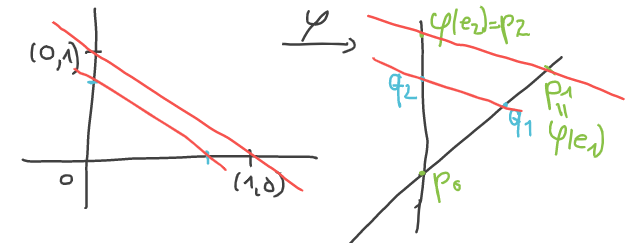
\includegraphics[width=0.5\linewidth]{figures/strahlensatz_koordinatensystem}
        \label{fig:strahlensatz_koordinatensystem}
    \end{figure}
    Sei
    \begin{align*}
        (\lambda,0)&=\inv{\phi}(q_1)\\
        (0,\mu)&=\inv{\phi}(q_2).
    \end{align*}    
    \begin{behauptung*}
        \( l_1=\inv{\phi}(q_1)\vee \inv{\phi}(q_2) \) und \( l_2=\inv{\phi}(p_1)\vee \inv{\phi}(p_2) \) sind parallel.
    \end{behauptung*}
    \minisec{Denn:}
    \begin{align*}
        T(l_1)&=K\vv{\inv{\phi}(q_1) \inv{\phi}(q_2)}\\
        T(l_2)&=K\vv{\inv{\phi}(p_1) \inv{\phi}(p_2)}.
    \end{align*}
    Es ist \( K\vv{p_1 p_2}=K\vv{q_1 q_2} \) und daher
    \begin{align*}
        \equalto{K\vv{\inv{\phi}(q_1) \inv{\phi}(q_2)}}{K \inv{\Phi}(\vv{p_1 p_2})}=\equalto{K\vv{\inv{\phi}(p_1) \inv{\phi}(p_2)}}{K\inv{\Phi}(\vv{q_1 q_2}}).
    \end{align*}
    Aus der Parallelität von \( l_1,l_2 \) folgt \( \lambda=\mu \).

    Also
    \begin{align*}
        &\rphantom{=}\teilverhaeltnis(\inv{\phi}(p_0),\inv{\phi}(p_1),\inv{\phi}(q_1))=\lambda\\
        &=\mu=\teilverhaeltnis(\inv{\phi}(p_0),\inv{\phi}(p_2),\inv{\phi}(q_2))
    \end{align*}
    und der Strahlensatz folgt aus \thref{teilverhaeltnis_invariant_unter_affinen_abbildungen}.
\end{proof}


% !TEX root = ./Vorlesungsmitschrift AGLA 2.tex  
\lecture{Di 05.05. 10:15}{}
\begin{lemma}\label{teilverhaeltnis_invariant_unter_affinen_abbildungen}
    Seien \( X,Y \) affine Räume und \( f\maps X\to Y \) eine affine Abbildung, seien \( p_0,p1,p \) Punkte in \( X \), die auf einer Geraden liegen und \( f(p_0)\neq f(p_1) \). Dann gilt
    \begin{align*}
        \teilverhaeltnis{f(p_0)}{f(p_1)}{f(p)}=\teilverhaeltnis{p_0}{p_1}{p}.
    \end{align*}
\end{lemma}
\begin{proof}
    Sei \( \lambda=\teilverhaeltnis{p_0}{p_1}{p} \), also \( \vv{p_0 p}=\lambda\vv{p_0 p_1} \). Sei \( F\maps T(X)\to T(Y) \) die zu \( f \) gehörige lineare Abbildung. Wir berechnen
    \begin{align*}
        \vv{f(p_0) f(p)}\begin{aligned}[t]
            &=F(\vv{p_0 p})\\
            &=F(\lambda{p_0 p_1})\\
            &=\lambda F({p_0 p_1})\\
            &=\lambda \vv{f(p_0) f(p_1)}
        \end{aligned}
    \end{align*}
    
\end{proof}
\begin{anwendung*}[Strahlensatz]
    Sei \( X \) ein affiner Raum über \( K \), \( p_0,p_1,p_2\in X \) affin unabhängig. Sei
    \begin{align*}
        q_1&\in p_0\vee p_1,\logicspace q_1\neq p_0\\
        q_2&\in p_0\vee p_2,\logicspace q_2\neq p_0.
    \end{align*}
    Wir nehmen an, dass \( p_1\vee p_2 \) und \( q_1\vee q_2 \) parallel sind in dem Sinn, dass
    \begin{align*}
        T(p_1\vee p_2)=T(q_1\vee q_2)\text{ in }T(X).
    \end{align*}
    Dann gilt
    \begin{align*}
        \teilverhaeltnis{p_0}{p_1}{q_1}=\teilverhaeltnis{p_0}{p_2}{q_2}.
    \end{align*}
    \begin{figure}[H]
        \centering
        \includegraphics[width=0.5\linewidth]{figures/Strahlensatz}
        \label{fig:Strahlensatz}
    \end{figure}
\end{anwendung*}
\begin{proof}
    Sei \( Y \) diedurch \( p_0,p_1,p_2 \) aufgespannte Ebene. Dann gibt es ein affines Koordinatensystem \( \phi\maps K^2 \to Y \) mit \( \phi(0)=p_0, \phi(e_1)=p_1, \phi(e_2)=p_2 \).
    \begin{figure}[H]
        \centering
        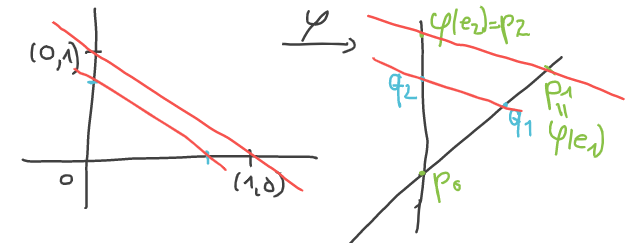
\includegraphics[width=0.5\linewidth]{figures/strahlensatz_koordinatensystem}
        \label{fig:strahlensatz_koordinatensystem}
    \end{figure}
    Sei
    \begin{align*}
        (\lambda,0)&=\inv{\phi}(q_1)\\
        (0,\mu)&=\inv{\phi}(q_2).
    \end{align*}    
    \begin{behauptung*}
        \( l_1=\inv{\phi}(q_1)\vee \inv{\phi}(q_2) \) und \( l_2=\inv{\phi}(p_1)\vee \inv{\phi}(p_2) \) sind parallel.
    \end{behauptung*}
    \minisec{Denn:}
    \begin{align*}
        T(l_1)&=K\vv{\inv{\phi}(q_1) \inv{\phi}(q_2)}\\
        T(l_2)&=K\vv{\inv{\phi}(p_1) \inv{\phi}(p_2)}.
    \end{align*}
    Es ist \( K\vv{p_1 p_2}=K\vv{q_1 q_2} \) und daher
    \begin{align*}
        \equalto{K\vv{\inv{\phi}(q_1) \inv{\phi}(q_2)}}{K \inv{\Phi}(\vv{p_1 p_2})}=\equalto{K\vv{\inv{\phi}(p_1) \inv{\phi}(p_2)}}{K\inv{\Phi}(\vv{q_1 q_2}}).
    \end{align*}
    Aus der Parallelität von \( l_1,l_2 \) folgt \( \lambda=\mu \).

    Also
    \begin{align*}
        &\rphantom{=}\teilverhaeltnis{\inv{\phi}(p_0)}{\inv{\phi}(p_1)}{\inv{\phi}(q_1)}=\lambda\\
        &=\mu=\teilverhaeltnis{\inv{\phi}(p_0)}{\inv{\phi}(p_2)}{\inv{\phi}(q_2)}
    \end{align*}
    und der Strahlensatz folgt aus \thref{teilverhaeltnis_invariant_unter_affinen_abbildungen}.
\end{proof}
\file{Affinkombinationen}
\section{Affinkombinationen}
\begin{beispiel*}
    Seien \( p_0,p_1\in \reals^2 \), \( p_0\neq p_1 \). Ziel: Beschreibe den affinen Unterraum \( p_0\vee p_1 \) als Teilmenge des \( \reals^2 \). Sei \( p\in p_0\vee p_1 \). Dann \( \exists \lambda\in \reals \) mit \( \vv{p_0 p}=\lambda \vv{p_0 p_1} \) und als Vektoren im \( \reals^2 \) gilt \( p=p_0+\lambda(p_1-p_0) \). Es gilt
    \begin{align*}
        p_0 \vee p_1=\Set{(1-\lambda)p_0+\lambda p_1,\logicspace \lambda\in \reals}.
    \end{align*}
    \begin{figure}[H]
        \centering
        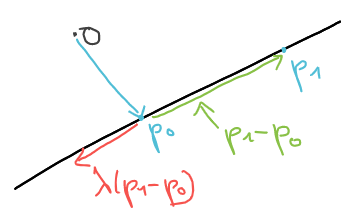
\includegraphics[width=0.5\linewidth]{figures/affine_verbindungsgerade}
        \label{fig:affine_verbindungsgerade}
    \end{figure}
    
\end{beispiel*}
\begin{frage*}
    Verallgemeinerung zu höherdimensionalen Räumen?
\end{frage*}
\begin{definition*}
    Seien \( p_0,\dotsc,p_k\in  K^n \). Wir nennen eine Linearkombination
    \begin{align*}
        \lambda_0 p_0+\lambda_1 p_1+\dotsb+\lambda_m p_m
    \end{align*}
    mit \( \lambda_i\in K \), \( 0\leq i\leq m \) eine Affinkombination oder affin falls gilt \( \lambda_0+\lambda_1+\dotsb+\lambda_m=1 \).
\end{definition*}
\begin{satz}
    Seien \( p_0,\dotsb,p_m\in K^n \). Dann gilt
    \begin{align*}
        p_0\vee \dotsb \vee p_m =\Set{\sum_{i=0}^{m}\lambda_i p_i\in K^n \logicspace \lambda_0,\dotsc,\lambda_m\in K, \sum_{i=0}^{m}\lambda_i=1}.
    \end{align*}
\end{satz}
\begin{proof}
    Sei \( Y=p_0 \vee\dotsb\vee p_m\in K^n \). Es gilt
    \begin{align*}
        T(Y)\begin{aligned}[t]
            &=\underbrace{T(p_m)}_{=0}+T(p_0\vee \dotsb \vee p_{m-1})+\underbrace{K\vv{p_0 p_m}}_{\mathclap{=T(p_0\vee p_m)}}\\
            &=K\vv{p_0 p_m}+T(p_0\vee \dotsb\vee p_{m-1})\\
            &=K\vv{p_0 p_m}+\dotsb +K\vv{p_0 p_1}\\
            &\vdots\\
            &=K\vv{p_0 p_m}+\dotsb + K\vv{p_0 p_1}\\
            &=\span(\vv{p_0 p_1}, \dotsc, \vv{p_0 p_m}).
        \end{aligned}
    \end{align*}
    Sei \( p\in K^n \). Dann ist \( p\in Y \) genau dann, wenn \texists \( \lambda_1,\dotsc,\lambda_m\in K \) mit
    \begin{align*}
        \vv{p_0 p}=\lambda_1 \vv{p_0 p_1}+\dotsb+\lambda_m\vv{p_0 p_m}.
    \end{align*}
    Im \( K^n \) gilt dann also
    \begin{align*}
        p-p_0=\lambda_1(p_1-p_0)+\dotsb + \lambda_m(p_m-p_0)
    \end{align*}
    oder 
    \begin{align*}
        p=\lambda_0 p_0+\lambda_1 p_1+\dotsb+\lambda_m p_m
    \end{align*}
    mit \( \lambda_0=1-\lambda_1-\dotsb-\lambda_m \), \dh \( \sum\limits_{i=0}^{m}\lambda_i=1 \).
\end{proof}
\file{Affine Abbildungen durch Matrizen, Fixpunkte}
\section{Affine Abbildungen und Matrizen, Fixpunkte}
\begin{motivation*}
    Seien \( V,W \) \( K \)-Vektorräume, \( F\maps V\to W \) eine lineare Abbildung. Wenn wir für \( V \) und \( W \) Basen wählen, dann können wir die Abbildung \( F \) eindeutig durch eine Matrix beschreiben.
\end{motivation*}
\begin{frage*}
    Inwiefern können wir affin Abbildung zwischen affinen Räumen durch Matrizen beschreiben?
\end{frage*}
Wahl von Basen in Vektorräumen \( \leftrightarrow \) Wahl von Koordinaten in affinen Räumen. 

Seien \( X,Y \) affine Räume über \( K \), \( f\maps X\to Y \) eine affine Abbildung. Wähle affine Koordinatensysteme \( \phi\maps K^n\to X  \) und \( \psi\maps K^m\to Y \).

Wir haben das folgende kommutative Diagramm
\begin{equation*}
    \begin{tikzcd}
        K^n\arrow{r}{\phi}\arrow{d}[name=g]{g} &X\arrow{d}[name=f]{f}\\
        K^m\arrow{r}{\psi}&Y
        \arrow[to path={(f) node[midway,scale=1] {\rotatebox{90}{\(\circlearrowright\)}} (g)}]{} 
    \end{tikzcd}    
\end{equation*}
mit \( g=\inv{\psi}\circ f\circ \phi \) affin. \( g \) ist affin, also besteht eine affine Abbildung \( G\maps K^n\to K^m \) mit
\begin{align*}
    g(x)-g(0)=G(x)\quad \forall x\in K^n.
\end{align*}
\( G \) ist linear, also können wir \( G \) durch eine Matrix \( A \) ausdrücken.
\begin{align*}
    g(x)=Ax+b\quad \forall x\in K^n.
\end{align*}
mit \( b=g(0) \).
\begin{frage*}
    Wie können wir \( A \) berechnen gegeben eine affine Basis \( (p_0,\dotsc,p_n) \) von \( K^n \) und \( g(p_i) \), \( 0\leq i \leq n \)?
\end{frage*}
\begin{figure}[H]
    \centering
    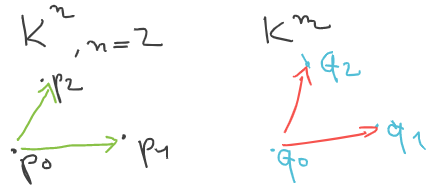
\includegraphics[width=0.5\linewidth]{figures/affine_basen_abbildung_wunsch}
    \label{fig:affine_basen_abbildung_wunsch}
\end{figure}
Wir betrachten die Matrizen \( B\in \matrices{m}{n}{K} \) bestehend aus den Spaltenvektoren \( \vv{q_0 q_1},\dotsc, \vv{q_0 q_n} \) und \( S\in \matrices{n}{n}{K} \) bestehend aus den Spaltenvektoren \( \vv{p_0 p_1}, \dotsc, \vv{p_0 p_n} \). Dann gilt \( A=B\cdot \inv{S}  \) und \( g(x)-g(p_0)=A(x-p_0) \), also \( g(x)=Ax+b \) mit \( b=g(p_0)-Ap_0 \).
\begin{bemerkung*}
    Wählen wir für \( p_0,\dotsc,pm \) die affine Basis \( 0,e_1,\dotsc, e_n \), dann \( S=\Id_{n\times n} \) und \( A=B \).
\end{bemerkung*}
\subsection*{Fixpunkte}
\begin{beispiel}
    Betrachte die affine Abbildung \( f\maps K\to K \), \( K \) ein Körper, in der Matrizendarstellung gegeben durch \( f(x)=2x+1\isittrue{=}x \).
    \begin{figure}[H]
        \centering
        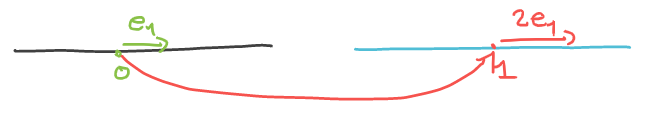
\includegraphics[width=0.5\linewidth]{figures/affiner_fixpunkt_1_d}
        \label{fig:affiner_fixpunkt_1_d}
    \end{figure}
    Dann gibt es genau ein \( x\in K \) mit \( f(x)=x \), nämlich \( x=-1 \).
\end{beispiel}
\begin{definition*}
    Sei \( X \) ein affiner Raum \( f\maps X\to X \) eine affine Abbildung. Wir nennen
    \begin{align*}
        \fixpunkte{f}\definedas \Set{x\in X|f(x)=x}
    \end{align*}
    die Menge der Fixpunkte von \( f \).
\end{definition*}
\begin{frage*}
    Welche Struktur hat \( \fixpunkte{f} \).
\end{frage*}
\begin{beispiel}
    \( X \) affiner Raum.
    \begin{align*}
        \Id\maps \begin{aligned}[t]
            X&\to X\\
            x&\mapsto x
        \end{aligned}
    \end{align*}
    dann \( \fixpunkte{\Id}=X \).
\end{beispiel}
\begin{beispiel}
    \( f\maps K^n\to K^n \), \( x\mapsto \underrelate{\isittrue{=}}{x}{\underbrace{x+p_0}} \) mit \( p_0\in K^n\setminus \zeroset \), dann \( \fixpunkte{f}=\emptyset \).
\end{beispiel}
\begin{beispiel}
    \begin{frage*}
        Was sind die Fixpunkte einer Projektion?
    \end{frage*}
    
\end{beispiel}
\begin{lemma}\label{affine_fixpunkte_sind_affiner_unterraum}
    \( \fixpunkte{f}\subseteq X \) ist ein affiner Unterraum.
\end{lemma}
\begin{proof}
    Falls \( \fixpunkte{f}=\emptyset \) dann \checkmark. Sei also \( \fixpunkte{f}\neq \emptyset \) und \( p\in \fixpunkte{f} \), \( F \) die zu \( f \) gehörig lineare Abbildung.

    Für \( x\in \fixpunkte{f} \) gilt
    \begin{align*}
        \vv{px}=\vv{f(p) f(x)}=F(\vv{px}).
    \end{align*}
    Umgekehrt folgt aus
    \begin{align*}
        \vv{px}=F(\vv{px})=\vv{p f(x)},
    \end{align*}
    dass \( x=f(x) \), also \( x\in \fixpunkte{f} \).

    Damit gilt
    \begin{align*}
        \Set{\vv{px}\in T(X)|x\in \fixpunkte{f}}=\Set{\vv{px}\in T(X)|\vv{px}=F(\vv{px})}
    \end{align*}
    und wir erkennen diese Menge als \( K \)-Untervektorraum von \( X \).
\end{proof}
\begin{frage*}
    Bestimmung von \( \fixpunkte{f} \) für eine beliebige affine Abbildung \( f\maps X\to X \)?
\end{frage*}
Nach Wahl eines Koordinatensystems können wir auf den Fall \( X=K^n \) reduzieren und annehmen, dass \( f \) in Matrizendarstellung gegeben ist.

Sei also
\begin{align*}
    f\maps \begin{aligned}[t]
        K^n&\to K^n\\
        x\mapsto &\underbrace{Ax+b}_{=x=\Id_n x}.
    \end{aligned}
\end{align*}
Dann gilt
\begin{align*}
    \fixpunkte{f}=\set{x\in K^n|(A-\explain{\text{Einheitsmatrix der Dimension \( n \):}\ \begin{pNiceMatrix}
        1 &  & 0 \\
         & \ddots &  \\
        0 &  & 1
    \end{pNiceMatrix}
    }{\Id_n})x=-b}
\end{align*}
Wir haben das Problem also reduziert auf das Lösen eines linearen Gleichungssystems.
\begin{bemerkung*}
    Daraus kann man auch \thref{affine_fixpunkte_sind_affiner_unterraum} ableiten.
\end{bemerkung*}
\begin{beispiel}\label{dilatation_beispiel}
    \begin{align*}
        f\maps \begin{aligned}[t]
            K^n&\to K^n\\
            x&\mapsto \lambda \Id_n x+b
        \end{aligned}     
    \end{align*}
    mit \( \lambda\in K \).

    Dann
    \begin{align*}
        \fixpunkte{f}=\Set{x\in K^n|(\lambda-1)x=-b}.
    \end{align*}
    Falls \( \lambda-1 \) invertierbar ist \( (\lambda\neq 1) \), gibt es genau einen Fixpunkt.
\end{beispiel}
\begin{definition*}
    Sei \( f\maps X\to X \) eine affine Abbildung mit zugehöriger linearer Abbildung \( F\maps T(X)\to T(X) \). Wir nennen \( f \) eine \emph{Dilatation} mit \emph{Faktor \( \lambda \)}, falls gilt
    \begin{align*}
        F=\lambda \cdot \Id_{T(X)}\quad \lambda\in K.
    \end{align*}
    Im Fall \( \lambda=1 \) nennen wir \( f \) eine Translation.
\end{definition*}
\begin{lemma}
    Sei \( f\maps X\to X \) eine Dilatation mit Faktor \( \lambda\neq 1 \). Dann gilt
    \begin{align*}
        \anzahl-{\fixpunkte{f}}=1.
    \end{align*}
\end{lemma}
\begin{proof}
    Nach Wahl eines Koordinatensystems reduzieren wir das Problem auf \thref{dilatation_beispiel}.    
\end{proof}
\file{Kollineationen}
\section{Kollineationen}
Sei \( f\maps X\to X \) eine affine Abbildung eines affinen Raumes \( X \), \zb eine Affinität. Seien \( p_1,p_2,p_3\subset X \) in einer Geraden \( \ell\subseteq X \) enthalten.
\begin{figure}[H]
    \centering
    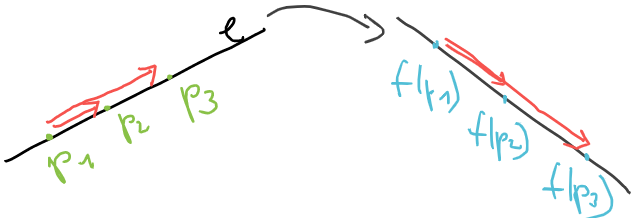
\includegraphics[width=0.5\linewidth]{figures/kollineationen_motivation}
    \label{fig:kollineationen_motivation}
\end{figure}
Dann liegen auch \( f(p_1), f(p_2),f(p_3) \) auf einer Geraden.

\begin{frage*}
    Welche bijektiven Abbildungen \( f\maps X\to X \) haben diese Eigenschaft?
\end{frage*}
\begin{definition*}
    Sei \( X \) ein affiner Raum und \( p_1,p_2,p_3\in X \). Wir nennen \( p_1,p_2,p_3 \) \emph{kollinear}, wenn \( p_1,p_2,p_3 \) auf einer Geraden \( \ell \subset X \) liegen. Wir nennen eine bijektive Abbildung \( f\maps X\to X \) eine Kollineation, falls jede Gerade \( \ell \subset X \) auf eine Gerade \( f(\ell)\subset X \) abgebildet wird.
\end{definition*}
\begin{beispiel}
    Affinitäten
\end{beispiel}
\begin{beispiel}
    Ist \( \affindim-{X}=1 \) und \( f\maps X\to X \) bijektiv, dann ist \( f \) eine Kollineation.
\end{beispiel}
\begin{beispiel}\label{kollinieationen:beispiele:komplexe_konjugation}
    Sei \( X=\complexs^2 \) als affiner Raum über \( \complexs \).
    \begin{align*}
        f\maps \begin{aligned}[t]
            \complexs^2\to \complexs^2\\
            (x,y)&\mapsto &(\explain{\text{komplexe Konjugation}}{\conjugate{x},\conjugate{y          }}).
        \end{aligned}
    \end{align*}
    Dann ist \( f \) eine Kollineation. Das Bild einer Geraden
    \begin{align*}
        (x_0,y_0)+\complexs(x_1,y_1)
    \end{align*}
    ist gegeben durch die Gerade
    \begin{align*}
        (\conjugate{x_0},\conjugate{y_0})+\complexs(\conjugate{x_1},\conjugate{y_1}),
    \end{align*}
    aber \( f \) ist \emph{keine Affinität}!
\end{beispiel}
\begin{bemerkung*}
    Die komplexe Konjugation
    \begin{align*}
        \begin{aligned}[t]
            \complexs&\to \complexs\\
            x&\mapsto \conjugate{x}
        \end{aligned}
    \end{align*}
    ist ein Automorphismus von dem Körper \( \complexs \).
\end{bemerkung*}
% !TEX root = ./Vorlesungsmitschrift AGLA 2.tex  
\lecture{Fr 08.05. 10:15}{}
\begin{definition*}
    Sei \( K \) ein Körper. Wir nennen eine Bijektion \( \alpha\maps K\to K \) einen Automorphismus von \( K \) falls gilt
    \begin{align*}
        \alpha(\lambda+\mu)&=\alpha(\lambda)+\alpha(\mu)\quad \forall \lambda,\mu\in K
        \intertext{und}
        \alpha(\lambda\cdot \mu)&=\alpha(\lambda)\cdot \alpha(\mu)\quad \forall  \lambda,\mu\in K
    \end{align*}
\end{definition*}
\begin{beispiel}
    \begin{align*}
        K=\rationals(\sqrt{2})=\Set{x+y\sqrt{2}|x,y\in\rationals}
    \end{align*}
    ist ein Körper und 
    \begin{align*}
        \alpha\maps \begin{aligned}[t]
            \rationals(\sqrt{2})&\to \rationals(\sqrt{2})\\
            x+y\sqrt{2}&\mapsto x-y\sqrt{2}.
        \end{aligned}
    \end{align*}
\end{beispiel}
\begin{satz}\label{alle_automorphismen_auf_r_identitaet}
    Sei \( \alpha\maps \reals\to \reals \) ein Automorphismus von \( \reals \). Dann gilt \( \alpha=\Id_{\reals} \).
\end{satz}
\begin{proof}
    Sei \( \alpha\maps \reals\to \reals \) ein Automorphismus.
    \begin{proofenumerate}
        \item Dann gilt
        \begin{align*}
            \alpha(0)=\alpha(0+0)=\alpha(0)+\alpha(0),
        \end{align*}
        also \( \alpha(0)=0 \).
        \item Dann gilt
        \begin{align*}
            0=\alpha(0)=\alpha(\lambda-\lambda)=\alpha(\lambda)+\alpha(-\lambda),
        \end{align*}
        also \( \alpha(-\lambda)=-\alpha(\lambda)\logicspace \forall \lambda\in \reals \).
        \item Dann gilt
        \begin{align*}
            \alpha(1)=\alpha(1\cdot 1)=\alpha(1)\alpha(1),
        \end{align*}
        also \( \alpha(1)=1 \) und daher
        \begin{align*}
            \alpha(n)=n\logicspace \forall n\in \wholes,
        \end{align*}
        \zb
        \begin{align*}
            \alpha(2)=\alpha(1+1)=\alpha(1)+\alpha(1)=1+1=2.
        \end{align*}
        \item Sei \( p\in \wholes \), \( q\in \naturals \), dann gilt
        \begin{align*}
            q\alpha\left( \frac{p}{q} \right)\begin{aligned}[t]
                &=\alpha(q)\alpha\left( \frac{p}{q} \right)=\alpha\left( q\frac{p}{q} \right)=\alpha(p)=p,
            \end{aligned}
        \end{align*}
        also \( \alpha\left( \frac{p}{q}=\frac{p}{q} \right) \) oder \( \alpha(t)=t\quad \forall t\in \rationals \).
        \item Sei \( \lambda\in \reals_{>0} \). Dann \texists  \( \mu\in\reals \) mit \( \lambda=\mu^2 \) und
        \begin{align*}
            \alpha(\lambda)=\alpha(\mu^2)=\alpha(\mu)\cdot \alpha(\mu)>0,
        \end{align*}
        also
        \begin{align*}
            \alpha(\lambda)>0\quad \forall \lambda\subset \reals>0.
        \end{align*}
    \end{proofenumerate}
    Wir zeigen nun \( \alpha(\lambda)=\lambda\quad \forall \lambda\in \reals \).

    \minisec{Gegenannahme}
    Sei \( \lambda\in \reals \) mit \( \alpha(\lambda)\neq \lambda \). Wir diskutieren den Fall \( \alpha(\lambda)<\lambda \) (\( \alpha(\lambda)>\lambda \) geht genauso).

    Wähle \( \frac{p}{q}\in \rationals \) mit
    \begin{align*}
        \alpha(\lambda)<\frac{p}{q}<\lambda.
    \end{align*}
    Dann gilt
    \begin{align*}
        \alpha(\lambda-\frac{p}{q})=\alpha(\lambda)-\frac{p}{q}<0
    \end{align*}
    \contra zu \( \lambda-\frac{p}{q}>0 \).
\end{proof}

\subsection*{Eine Familie von Kollineationen}
\begin{idee*}
    Wir verallgemeinern \thref{kollinieationen:beispiele:komplexe_konjugation}, um eine größere Klasse an Kollineationen zu erhalten als Affinitäten.
\end{idee*}
\begin{beispiel}
    \begin{align*}
        f\maps \begin{aligned}[t]
            \complexs^2&\to \complexs^2\\
            (x,y)&\mapsto (\conj{x},\conj{y})
        \end{aligned}
    \end{align*}
    respektiert Addition, \dh
    \begin{align*}
        f(z+z')=f(z)+f(z')\quad \forall z,z'\in \complexs^2,
    \end{align*}
    und hat die Eigenschaft
    \begin{align*}
        f(\lambda z)=\conj{\lambda} f(z)\quad \forall \lambda\in \complexs\logicspace \forall z\in \complexs^2.
    \end{align*}
    \tto Wir nennen \( f \) semilinear.
\end{beispiel}
\begin{definition*}
    Seien \( V,W \) Vektorräume über einem Körper \( K \). Wir nennen eine Abbildung \( F\maps V\to W \) \emph{semilinear}, wenn es einen Automorphismus \( \alpha \) von \( K \) gibt, sodass gilt
    \begin{itemize}
        \item \(F(v+v')=F(v)+F(v')\quad \forall v,v'\in V\)
        \item \( F(\lambda v)=\alpha(\lambda) F(v)\quad \forall \lambda\in K \logicspace \forall v\in V\).
    \end{itemize}
\end{definition*}
\begin{definition*}
    Seien \( X,Y \) affine Räume über einem Körper \( K \). Wir nennen eine Abbildung
    \begin{align*}
        f\maps X\to Y
    \end{align*}
    \emph{semiaffin}, wenn es eine \emph{semilineare Abbildung} \( F\maps T(X)\to T(Y) \) gibt mit
    \begin{align*}
        \vv{f(p) f(q)}=F(\vv{pq})\logicspace \forall p,q\in X.
    \end{align*}
    Falls \( f \) außerdem bijektiv ist, dann nennen wir \( f \) eine Semiaffinität.
\end{definition*}
\begin{lemma}
    Sei \( f\maps X\to X \) eine Semiaffinität eines affinen Raumes \( X \). Dann ist \( f \) eine Kollineation.
\end{lemma}
\begin{proof}[Beweisidee]
    Sei \( \ell \subseteq X \) eine Gerade, \( p_0\in \ell \). Dann ist
    \begin{align*}
        T(\ell)=\Set{\vv{p_0 x}, x\in \ell}\subseteq T(x)
    \end{align*}
    ein \( K \)-Untervektorraum mit
    \begin{align*}
        \dim_K T(\ell)=1.
    \end{align*}
    Sei \( F\maps T(X)\to T(X)  \) die zu \( f \) gehörige semilineare Abbildung.

    Wir betrachten 
    \begin{align*}
        T(f(\ell))
        \begin{aligned}[t]
            &=\Set{\vv{f(p_0) f(x), x\in \ell}}\\
            &=\Set{F(\vv{p_0 x}), x\in \ell}
            &=F(T(\ell)).
        \end{aligned}        
    \end{align*}
    Dann ist auch \( F(T(\ell))\subseteq T(X) \) ein \( \explain{\text{Übung}}{K \text{-Untervektorraum}} \) der Dimension \( 1 \), also
    \begin{align*}
        f(\ell)\subseteq X
    \end{align*}
    eine Gerade.
\end{proof}
\begin{frage*}
    Gibt es Kollineationen, die keine Semiaffinität sind?
\end{frage*}
\tto Ja, \zb für \( \dim X=1 \).
\subsection*{Hauptsatz der affinen Geometrie}

Sei \( K \) ein Körper mit \( \anzahl K\geq 3 \), \( X \) ein affiner Raum über \( K \) mit \( \dim X\geq 2 \) und \( f\maps X\to X \) eine Kollineation. Dann ist \( f \) eine Semiaffinität.

\begin{bemerkung*}
    Aus \thref{alle_automorphismen_auf_r_identitaet} folgt, dass über \( \reals \) jede semilineare Abbildung linear ist.
\end{bemerkung*}
\begin{korollar*}
    Sei \( X \) ein affiner Raum über \( \reals \) mit \( \dim X\geq 2 \), \( f\maps X\to X \) eine Kollineation. Dann ist \( f \) eine Affinität.
\end{korollar*}

\section{Quadriken}
\begin{motivation*}
    Affine Unterräume der \( \reals^n \) sind gegeben durch \emph{lineare} Gleichungssysteme.
\end{motivation*}
\minisec{Jetzt:}
Betrachte den Unterraum im \( \reals^n \), der entsteht als Lösungsmenge einer \emph{quadratischen} Gleichung.
\begin{beispiele*}[im \( \reals^2 \)]
    \begin{enumerate}
        \item der Kreis
        \begin{align*}
            \Set{(x,y)\in \reals^2|x^2+y^2=1}
        \end{align*}
        \item Ellipsen, \( a,b>0 \)
        \begin{align*}
            E=\Set{(x,y)\in \reals^2|ax^2+by^2=1}
        \end{align*}
        \begin{figure}[H]
            \centering
            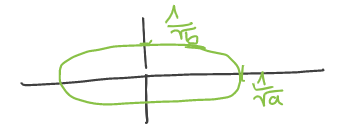
\includegraphics[width=0.5\linewidth]{figures/quadriken_beispiel_ellipse}
            \label{fig:quadriken_beispiel_ellipse}
        \end{figure}
        \item Parabel
        \begin{align*}
            y=ax^2
        \end{align*}
        \begin{figure}[H]
            \centering
            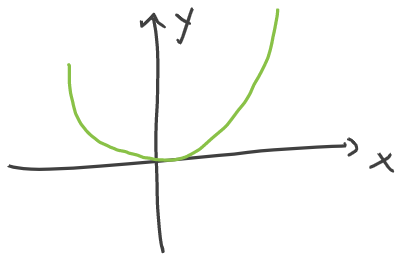
\includegraphics[width=0.5\linewidth]{figures/quadriken_beispiel_parabel}
            \label{fig:quadriken_beispiel_parabel}
        \end{figure}
        \item Hyperbeln, \( a,b>0 \)
        \begin{align*}
            ax^2-by^2=1 
        \end{align*}
        \begin{figure}[H]
            \centering
            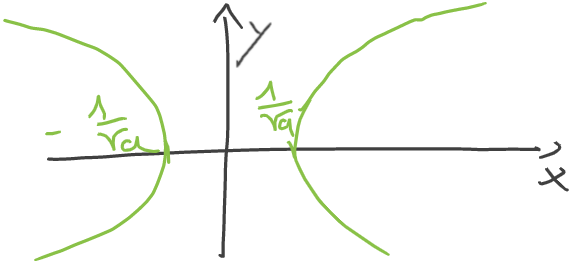
\includegraphics[width=0.5\linewidth]{figures/quadriken_beispiel_hyperbeln}
            \label{fig:quadriken_beispiel_hyperbeln}
        \end{figure}
        \item \( x^2=0 \)
        \begin{figure}[H]
            \centering
            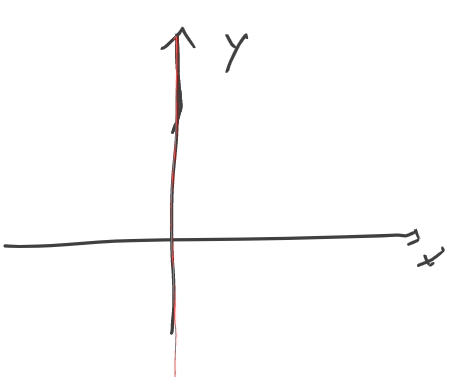
\includegraphics[width=0.4\linewidth]{figures/quadriken_beispiel_y_achse}
            \label{fig:quadriken_beispiel_y_achse}
        \end{figure}
        \item \( xy=0 \)
        \begin{figure}[H]
            \centering
            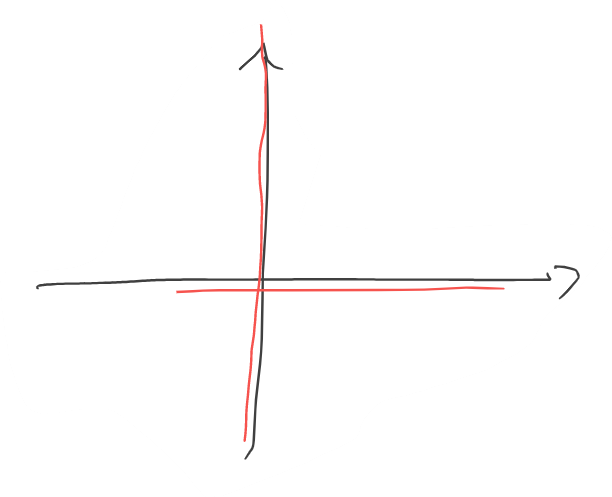
\includegraphics[width=0.4\linewidth]{figures/quadriken_beispiel_x_achse_und_y_achse}
            \label{fig:quadriken_beispiel_x_achse_und_y_achse}
        \end{figure}
        \item \( x^2+y^2=0 \)
        \begin{figure}[H]
            \centering
            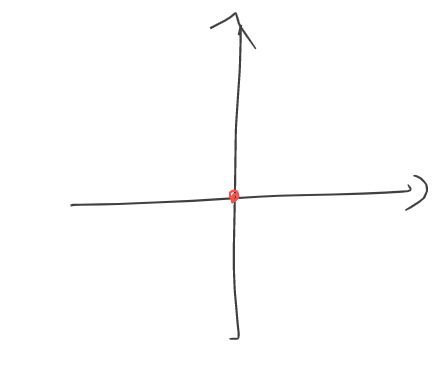
\includegraphics[width=0.4\linewidth]{figures/quadriken_beispiel_ursprung}
            \caption*{Der Ursprung}
            \label{fig:quadriken_beispiel_ursprung}
        \end{figure}
    \end{enumerate}
\end{beispiele*}
\begin{beispiele*}
    Sei \( Q\subseteq \reals^2 \) gegeben durch
    \begin{align*}
        x_1^2+2x_1x_2+2x_2^2+2x_1=0.
    \end{align*}
    Erster Schritt: Entferne den \enquote{gemischten} Term \( x_1 x_2 \).
    \begin{align*}
        (x_1+x_2)^2+x_2^2+2x_1=0.
    \end{align*}
    Nach der Koordinatentransformation
    \begin{align*}
        y_1=x_1+x_2\quad y_2=x_2
    \end{align*}
    ist \( Q \) gegeben durch
    \begin{align*}
        y_1^2+y_2^2+2y_1\cdot 1-2y_2\cdot 1=0.
    \end{align*}
\end{beispiele*}
\begin{bemerkung*}
    Wir können die obigen Gleichungen auch über anderen Körpern \( K \) betrachten, die Lösungsmenge hängt im Allgemeinen wesentlich von \( K \) ab, \zb \( x^2+y^2=0 \).
    \begin{frage*}
        Was passier hier über \( \complexs \), \( \quot{\wholes}{p\wholes} \) für \( p \) prim?
    \end{frage*}
\end{bemerkung*}
\begin{definition*}
    Sei \( K  \) ein Körper. Ein quadratisches Polynom über \( K \) in den Unbestimmten \( x_1,\dotsc, x_n \) ist eine Ausdruck der Form
    \begin{align*}
        P(x_1,\dotsc, x_n)=\sum_{1\leq i, j\leq n} \alpha_{ij}x_i x_j+\sum_{1\leq i\leq n} \alpha_{0i} x_i+\alpha_{00}.
    \end{align*} 
    mit \( \alpha_{ij},\alpha_{0i}, \alpha_{00}\in K \quad \forall 1\leq i,j\leq n \).
\end{definition*}
\begin{bemerkung*}
    Aus einem quadratischen Polynom \( P \) über \( K \) erhält man eine Abbildung
    \begin{align*}
        K^n&\to K\\
        (t_1,\dotsc,t_n)&\mapsto P(t_1,\dotsc,t_n).
    \end{align*}
\end{bemerkung*}
\begin{achtung*}
    Zwei unterschiedliche Polynome \( P_1,P_2 \) müssen nicht notwenigerweise identisch sein, um dieselben Abbildung zu induzieren.
\end{achtung*}
\begin{beispiel*}
    \( K=\mathbb{F}_p=\quot{\wholes}{p\wholes} \). Körper mit \( p \) Elementen mit \( p \) prim, \( n=1 \).
    \begin{align*}
        P_1&=x\\
        P_2&=x^p.
    \end{align*}
    Nach Fermats kleinem Satz gilt
    \begin{align*}
        t\equiv t^p \mod p\quad \forall t\in \quot{\wholes}{p\wholes}.
    \end{align*}
    Für \( p=2 \) sind \( P_1,P_2 \) quadratische Polynome nach obiger Definition.
\end{beispiel*}
\begin{definition*}
    Wir nennen eine Teilmenge \( Q\subseteq K^n \) eine \emph{Quadrik}, falls \( Q \) definiert ist durch
    \begin{align*}
        Q=\Set{(x_1,\dotsc,x_n)\in K^n|P(x_1,\dotsc,x_n)=0}
    \end{align*}
    für ein quadratisches Polynom \( P \) über \( K \).
\end{definition*}
\begin{beispiele*}
    \begin{itemize}
        \item \( x_1^2+\dotsb+x_n^2=0 \) über \( \reals \) ergibt den Ursprung.
        \item \( a_1x_1^2+\dotsb+a_n x_n^2=1 \), \( a_1,\dotsb,a_n>0 \) über \( \reals \) ergibt einen Ellipsoid.
        \item \( K=\reals \), \( P=x_1^2+2x_1x_2+5x_2^2 \). Dann ist
        \begin{align*}
            Q=\Set{x_1,x_2\in \reals^2|\underbrace{(x_1,x_2)\begin{pNiceMatrix} 1 & \underline{1} \\ \underline{1} & 5 \end{pNiceMatrix}\begin{pNiceMatrix} x_1 \\ x_2 \end{pNiceMatrix}=0}_{P(x_1,x_2)}}.
        \end{align*}
    \end{itemize}
\end{beispiele*}
\begin{frage*}
    Wie können wir im Allgemeinen Quadriken in Matrizenschreibweise ausdrücken?
\end{frage*}









% !TEX root = ./Vorlesungsmitschrift AGLA 2.tex  
\lecture{Di 12.05. 10:15}{}
\renewcommand{\transpose}[1]{\leftidx{^t}{#1}{}}
\begin{idee*}
  Sei
  \begin{align*}
    P(x_1,\dotsc,x_n)=\sum\limits_{1\leq i\leq j\leq n}\alpha_{ij}x_i x_j+\sum\limits_{1\leq i \leq n}\alpha_{0i}x_i\cdot 1+\alpha_{00}\cdot 1^2.
  \end{align*}
  Wir schreiben
  \begin{align*}
    x'=\begin{pNiceMatrix} 1\\ x_1 \\ \vdots \\ x_n \end{pNiceMatrix}\in K^{n+1}.
  \end{align*}
  und (sei im Folgenden \( \characteristic K\neq 2 \))
  \begin{align*}
    A=\begin{pNiceArray}{C|CCCC}
      a_{00}& a_{01} & \Cdots & \Cdots & a_{0n} \\
      \hline
      a_{10} & a_{11} & a_{12} & \Cdots & a_{1n} \\
       \Vdots & \Vdots & \Ddots &  & \Vdots \\
       \\
       a_{n0} & a_{n1} & \Cdots & \Cdots & a_{nn}
    \end{pNiceArray}
  \end{align*}
  mit \( a_{ii}=\alpha_{ii}\quad \forall 0\leq i\leq n \).
  \begin{align*}
    a_{ij}=a_{ji}=\frac{1}{2}\alpha_{ij}\text{ für }0\leq i<j\leq n.
  \end{align*}
  Es gilt dann
  \begin{align*}
    P(x_1,\dotsc,x_n)=\transpose{x'}A'x'
  \end{align*}
  und
  \begin{equation*}
    Q=\Set{(x_1,\dotsc,x_n)\in K^n| \transpose{x'}A'x'=0}.
  \end{equation*}
\end{idee*}
\begin{bemerkung*}
  Die Matrix \( A' \) ist symmetrisch (nach Konstruktion).
\end{bemerkung*}
\begin{definition*}
  In obiger Notation nennen wir \( A' \) di erweiterte Matrix zu \( P \) und \( x' \) den erweiterten Spaltenvektor zu \( x \). Wir sagen, dass \( A'\in \Mat_{(n+1)\times(n+1)}(K) \) die Quadrik \( Q \) beschreibt, wenn gilt
  \begin{equation*}
    Q=\Set{x\in K^n|\transpose{x'}A'x'=0}.
  \end{equation*}
\end{definition*}
\begin{notation*}
  Für \( P \) wie oben schreiben wir
  \begin{equation*}
    A=\begin{pNiceMatrix}
      a_{11} & \Cdots & a_{1n} \\
      \Vdots &  & \Vdots \\
      a_{n1} & \Cdots & a_{nn}
    \end{pNiceMatrix}
  \end{equation*}
  für den \enquote{rein quadratischen} Anteil von \( P \).
\end{notation*}
\begin{bemerkung*}
  Sei \( Q\subseteq K^n \) eine Quadrik. Dann gibt es im Allgemeinen nicht nur eine erweiterte Matrix \( A' \) die \( Q \) beschreibt. Ist
  \begin{equation*}
    Q=\Set{(x_1,\dotsc,x_n)\in K^n| \transpose{x'}A'x'=0},
  \end{equation*}
  dann beschreibt auch \( \lambda A' \) mit \( \lambda\in K\setminus\zeroset \) die Quadrik \( Q \).
\end{bemerkung*}
\begin{frage*}
  Wie verhalten sich Quadriken unter Koordinatentransformationen / Affinitäten?
\end{frage*}
\begin{beispiel*}
  \( K=\rationals \). \( P(x_1,x_2)=x_1^2+x_2^2 \).
  \begin{align*}
    \begin{pNiceMatrix} x_1 \\ x_2 \end{pNiceMatrix}&\begin{aligned}[t]
      &=\begin{pNiceMatrix} y_1+y_2 \\ y_2+1 \end{pNiceMatrix}\\
      &=\begin{pNiceMatrix} 1 & 1 \\ 0 & 1 \end{pNiceMatrix}\begin{pNiceMatrix} y_1 \\ y_2 \end{pNiceMatrix}+\begin{pNiceMatrix} 0 \\ 1 \end{pNiceMatrix}.
    \end{aligned}\\
    P(x_1,x_2)&\begin{aligned}[t]
      &=(y_1+y_2)^2+(y_2+1)^2\\
      &=y_1^2+2y_1 y_2+2 y_2^2+2y_2+1
    \end{aligned}
  \end{align*}
  ist wieder ein quadratisches Polynom.
\end{beispiel*}
\begin{lemma}\label{affinitaet_bildet_quadriken_auf_quadriken_ab}
  Sei \( K \) ein Körper mit \( \characteristic K\neq2 \), \( Q\leq K^n \) eine Quadrik und \( f\maps K^n\to K^n \) eine Affinität. Dann ist auch \( f(Q)\subseteq K^n \) eine Quadrik.
\end{lemma}
\begin{proof}
  Sei \( Q \) gegeben durch das quadratische Polynom \( P(x_1,\dotsc, x_n) \), also
  \begin{equation*}
    Q=\Set{(x_1,\dotsc,x_n)\in K^n|P(x_1,\dotsc,x_n)=0}.
  \end{equation*}
  Sei \( A' \) die erweiterte Matrix zu \( P \) und \( x' \) der erweiterte Spaltenvektor zu \( x \). Dann gilt
  \begin{align*}
    Q=\Set{(x_1,\dotsc,x_n\in K^n)|\transpose{x'}A'x'=0}.
  \end{align*}
  Als nächstes beschreibe den durch \( f \) gegebenen Koordinatenwechsel. \( f \) ist eine Affinität, also \texists \( b\in K^n \) und \( S\in \GL_n(K) \) mit
  \begin{equation*}
    \begin{split}
      f\maps K^n&\to K^n\\
      x&\mapsto Sx+b.
    \end{split}
  \end{equation*}
  Sei \( y=f(x) \), schreibe \( y'=\begin{pNiceMatrix} 1 \\ y_1 \\ \Vdots \\ y_n \end{pNiceMatrix} \),
  \begin{equation*}
    S'=\begin{pNiceArray}{C|CCC}
      1 & 0 & \Cdots & 0 \\\hline
      b_1 & \Block{3-3}<\LARGE>{S} &  & \\
      \Vdots & & & \\
      b_n & & &
    \end{pNiceArray}.
  \end{equation*}
  Dann gilt \( y'=S'x' \).
  \begin{bemerkung*}
    \( S' \) ist invertierbar mit inverser Matrix
    \begin{equation*}
      T'=\inv{(S')}=\begin{pNiceArray}{C|CCC}
        1 & 0 & \Cdots & 0 \\\hline
         & \Block{3-3}<\LARGE>{\inv{S}} &  & \\
         -\inv{S}b & & & \\
         & & &
      \end{pNiceArray},
    \end{equation*}
    \dh \( x'=T'y' \).
  \end{bemerkung*}
  Es gilt
  \begin{equation*}
    \begin{split}
      f(Q)&=\Set{f((x_1,\dotsc,x_n))\in K^n| P(x_1,\dotsc,x_n)=0}\\
      &=\Set{y\in K^n| \transpose{x'}A'x'=0}\\
      &=\Set{y\in K^n| \transpose{(T'y')}A'(T'y')=0}\\
      &=\Set{y\in K^n| \transpose{y'}\underbrace{\transpose{T'}A'T'}_{\mathclap{\text{symmetrische Matrix}}}y'=0},
    \end{split}
  \end{equation*}
  also ist \( f(Q) \) eine Quadrik mit
  \begin{equation*}
    P'(y_1,\dotsc, y_n)=\transpose{y'}(\transpose{T'}A'T')y'.
  \end{equation*}
\end{proof}
\begin{bemerkung*}
  Der Beweis von \thref{affinitaet_bildet_quadriken_auf_quadriken_ab} zeigt wie sich eine beschreibende Matrix \( A' \) unter einer Koordinatentransformation ändert.
\end{bemerkung*}
\begin{frage*}
  Sei \( Q \) eine Quadrik beschrieben durch eine erweiterte Matrix \( A' \). Find eine Koordinatentransformation \( f \) der \( K^n \), sodass \( f(Q) \) möglichst \enquote{einfach} beschrieben werden kann.
\end{frage*}
\minisec{zweiter Schritt}
Entferne lineare Terme
\begin{equation*}
  (y_1+1)^2+(y_2-1)^2-2=0.
\end{equation*}
Nach der Koordinatentransformation
\begin{equation*}
  z_1=y_1+1\qquad z_2=y_2-1
\end{equation*}
erhalten wir \( z_1^2+z_2^2=2 \), oder nach skalieren mit \( \sqrt{2} \)
\begin{gather*}
  \sqrt{2}w_1= z_1\qquad \sqrt{2}w_2=z_2\\
  w_1^2+w_2^2=1
\end{gather*}
\begin{figure}[H]
  \centering
  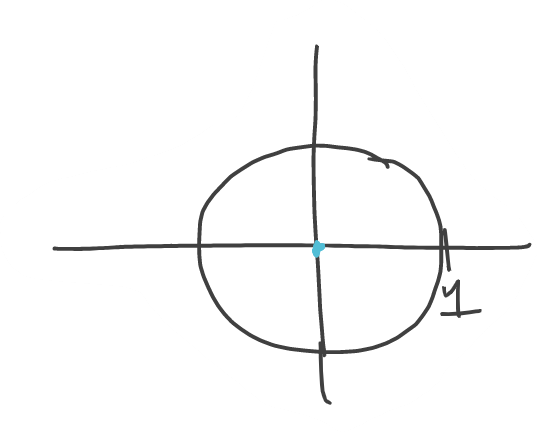
\includegraphics[width=0.5\linewidth]{figures/vereinfachte_quadrik}
  \label{fig:vereinfachte_quadrik}
\end{figure}
\begin{satz}[affine Hauptachsentransformation von reellen Quadriken]\label{affine_hauptachsentranformation_reelle_quadriken}
  Sei \( A'\in \Mat_{(n+1)\times(n+1)}(\reals) \) eine symmetrische Matrix und die Quadrik \( Q\subseteq \reals^n \) gegeben durch
  \begin{equation*}
    Q=\Set{(x_1,\dotsc,x_n)\in \reals^n|\transpose{x'}A'x'=0}.
  \end{equation*}
  Sei \( A \) der rein quadratische Anteil von \( A' \), \( m=\rang A \) und \( m'=\rang A' \). Dann gibt es eine Affinität \( f\maps \reals^n\to \reals^n \), sodass \( f(Q) \) beschrieben wird durch eine der folgenden Gleichungen:
  \begin{eigenschaftenenumerate}
    \item \( m=m' \):
    \begin{equation*}
      y_1^2+\dotsb+y_k^2-y_{k+1}^2-\dotsb-y_m^2=0
    \end{equation*}
    für ein \( 0\leq j \leq m \).
    \item \( m+1=m' \):
    \begin{equation*}
      y_1^2+\dotsb+y_k^2-y_{k+1}^2-\dotsb-y_m^2=1
    \end{equation*}
    für ein \( 0\leq k \leq m \).
    \item \( m+2=m' \):
    \begin{equation*}
      y_1^2+\dotsb+y_k^2-y_{k+1}^2-\dotsb-y_m^2+2_{y_{m+1}}=0
    \end{equation*}
    für ein \( 0\leq k\leq m \).
  \end{eigenschaftenenumerate} 
\end{satz}
\begin{frageuebung}
  Warum gilt immer \( m\leq m'\leq m+2 \)?
\end{frageuebung}
\begin{proof}[Beweis zu \thref{affine_hauptachsentranformation_reelle_quadriken}]
  Sei
  \begin{equation*}
    A'=\begin{pNiceArray}{C|CCC}
      a_{00} & a_{01} & \Cdots & a_{0n} \\\hline
      a_{10} & \Block{3-3}<\LARGE>{A} &  & \\
      \Vdots & & & \\
      a_{n0} & & &
    \end{pNiceArray}.
  \end{equation*}
  mit \( A\in \Mat_{n\times n}(\reals) \).
  \begin{proofenumerate}[label=Schritt \arabic*]
    \item Entferne gemischte Terme.
    \begin{idee*}
      Wollen \( A \) in Diagonalgestalt bringen. 
    \end{idee*}
    AGLA \Romannum{1}: Orthogonalisierungssatz für reelle symmetrische Matrizen.

    Wir erhalten eine invertierbare Matrix \( T_1\in \GL_n(\reals) \) mit
    \begin{equation*}
        \transpose{T_1}AT_1=\begin{pNiceArray}{C|C|C}
            I_k & 0 & 0\\\hline
            0 & -I_{m-k} & 0\\\hline
            0 & 0 & 0
        \end{pNiceArray},
    \end{equation*}
    \( I_l \) Einheitsmatrix der Dimension \( l \), \( m=\rang A \), \( k \) Zahl der positiven Eigenwerte von \( A \) (mit Vielfachheit).

    Sei
    \begin{equation*}
      T_1'=\begin{pNiceArray}{C|CCC}
        1 & 0 & \Cdots & 0 \\\hline
        0 & \Block{3-3}<\LARGE>{T_1} &  & \\
        \Vdots & & & \\
        0 & & &
      \end{pNiceArray}.
    \end{equation*}
    Dann gilt
    \begin{equation*}
      \begin{split}
        A_1'&\definedas \transpose{T_1'}A'T_1'\\
        &=\begin{pNiceArray}{C|CCC}[create-large-nodes]
          c_{00} & c_{01} & \Cdots & c_{0n} \\\hline
          c_{10} & I_k   & 0   &0    \\\cline{2-4}
          \Vdots & 0  & -I_{m-k}   &0 \\\cline{2-4}
          c_{n0} & 0    & 0    & 0
          \CodeAfter
            \tikz \draw (2-2-large.north east) -- (4-2-large.south east);
            \tikz \draw (2-3-large.north east) -- (4-3-large.south east);
        \end{pNiceArray}
      \end{split}
    \end{equation*}
    für \( c_{00}, c_{01}, \dotsc,c_{0n}, c_{1 0},\dotsc, c_{n 0} \in \reals\) mit \( c_{i0}=c_{0i} \) \tforall \( i \). Die durch \( A' \) bestimmte Quadrik ist gegeben durch
    \begin{equation*}
      y_1^2+\dotsb+y_k^2-y_{k+1}^2-\dotsb-y_m^2+2(c_{01}y_1+\dotsb+c_{0n} y_n)+c_{00}=0.
    \end{equation*}
    \item Reduzieren der linearen Terme. Sei
    \begin{equation*}
      T_2'=\begin{pNiceArray}{C|CCCCCCCCC}
        1 & 0 & \Cdots & & & &&&&0 \\\hline
        -c_{10} & 1 & & & &\Block{4-4}<\Large>{0} \\
        \Vdots & &\Ddots \\
        -c_{k 0} \\
        c_{(k+1)0}\\
        \Vdots\\
        c_{m0}&\Block{4-4}<\Large>{0}\\
        0\\
        \Vdots \\
        0 &&&&&&&&&1
      \end{pNiceArray}
    \end{equation*}
    entsprechend dem Basiswechsel
    \begin{equation*}
      y_i=\begin{cases}
        z_i-c_{i0} & 1\leq i \leq k\\
        z_i+c_{i0} & k<i\leq m\\
        z_i &i>m.
      \end{cases}
    \end{equation*}
    Sei
    \begin{equation*}
      \begin{split}
        A_2'&\definedas \transpose{T_2'}A_1'T_2'\\
        &=\begin{pNiceArray}{C|CCCC|CCC}[create-large-nodes]
          d_{00} & 0 & \Cdots & & 0 & c_{0(m+1)} & \Cdots & c_{0 n}\\\hline
          0 & \Block{2-2}<\large>{I_k}\phantom{-IO} & & \Block{2-2}<\large>{0}\phantom{-IOO} & & \Block{4-3}<\LARGE>{0} \\
          \Vdots &&&&&&&\\\cline{2-5}
          & \Block{2-2}<\large>{0}\phantom{-IOO} & & \Block{2-2}<\large>{-I_{m-k}} &&&&\\
          0&&&&&&\\\hline
          c_{(m+1)0} & \Block{3-4}<\LARGE>{0} & & & &\Block{3-3}<\LARGE>{0}\\
          \Vdots&&&&&&&\\
          c_{n 0}&&&&&&&
          \CodeAfter
            \tikz \draw (2-4-block.north west) --  (4-4-block.south west);
        \end{pNiceArray}.
      \end{split}
    \end{equation*}
    Nach der durch \( T_1'T_2' \) beschriebenen Koordinatentransformation ist \( Q \) gegeben durch
    \begin{multline*}
      z_1^2+\dotsb+z_k^2-z_{k+1}^2-\dotsb-z_m^2+2(c_{(m+1)0}z_{m+1}+\dotsb+c_{n0}z_n)+d_{00}.
    \end{multline*}
    \minisec{Fallunterscheidung}
    \begin{eigenschaftenenumerate}
      \item \( d_{00}=c_{(m+1)0}=\dotsb=c_{n0}=0 \).
      \item \( d_{00}\neq 0 \), \( c_{(m+1)0}=\dotsb=c_{n0}=0 \). Nach eventuellem Multiplizieren der Matrix \( A' \) mit \( (-1) \) und Umordnen der Variablen \( z_i \), können wir \( d_{00}<0 \) annehmen.

      Sei \( \lambda=\sqrt{\abs*{d_{00}}} \) und definiere
      \begin{equation*}
        T_3'=\begin{pNiceArray}{C|CCC}
          1 & 0 & \Cdots & 0\\\hline 
          0 & \Block{3-3}{\lambda I_n}\\
          \Vdots \\
          0
        \end{pNiceArray}.
      \end{equation*}
      Wir berechnen
      \begin{equation*}
        A_3'\definedas \transpose{T_3'}A_2'T_3'.
      \end{equation*}
      Dann ist
      \begin{equation*}
        A_3'=\begin{pNiceArray}{C|CCC}[create-large-nodes]
          -\lambda^2 & 0 & \Cdots & 0 \\\hline
          0 & \lambda^2 I_k   & 0   &0    \\\cline{2-4}
          \Vdots & 0  & -\lambda^2 I_{m-k}   &0 \\\cline{2-4}
          0 & 0    & 0    & 0
          \CodeAfter
            \tikz \draw (2-2-large.north east) -- (4-2-large.south east);
            \tikz \draw (2-3-large.north east) -- (4-3-large.south east);
        \end{pNiceArray}.
      \end{equation*}
      Nach der zu \( T_1' t_2' t_3' \) gehörigen Affinität und Division durch \( \lambda^2 \) wird \( Q \) gegeben durch
      \begin{equation*}
        u_1^2+\dotsb+u_k^2-u_{k+1}^2-u_m^2=1.
      \end{equation*}
      \item \( c_{i0}\neq 0 \) für mindestens ein \( m+1\leq i\leq n \). Nach Umordnen der Variablen \( z_i \), \( m+1\leq i \leq n \) können wir annehmen, dass \( c_{(m+1)0}\neq 0 \) gilt. Betrachte die Koordinatentransformation \( u_i=z_i \), \( i\neq m+1. \),
      \begin{equation*}
        2u_{m+1}=2(c_{(m+1)0}z_{m+1}+\dotsb+c_{n0}z_n)+d_{00}.
      \end{equation*}
      Nach dieser Affinität wird \( Q \) beschrieben durch
      \begin{equation*}
        u_1^2+\dotsb+u_k^2-u_{k+1}^2-\dotsb-u_m^2+2u_{m+1}=0.
      \end{equation*}
    \end{eigenschaftenenumerate}
  \end{proofenumerate}
\end{proof}
% !TEX root = ./Vorlesungsmitschrift AGLA 2.tex  
\lecture{Fr 15.05. 10:15}{}
Resultate der affinen Hauptachsentransformation im \( \reals^2 \): \( m=\rang A \), \( m'=\rang A' \).
\begin{eigenschaftenenumerate}
  \item \( m=m' \):
  \begin{proofdescription}
    \item[\( m=m'=0 \):] \( Q \) gegeben durch \( 0=0 \) \tto Ebene \( \reals^2 \).
    \item[\( m=m'=1 \)] \( x_1^2=0 \) \tto \enquote{doppelte} Gerade. 
    \begin{figure}[H]
      \centering
      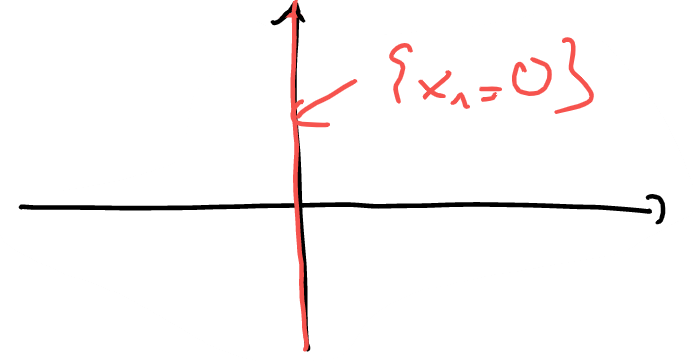
\includegraphics[width=0.5\linewidth]{figures/doppelte_gerade}
      \label{fig:doppelte_gerade}
    \end{figure}
    \item[\( m=m'=2 \)] \( x_1^2+x_2^2=0 \) \tto Punkt.
    \begin{figure}[H]
      \centering
      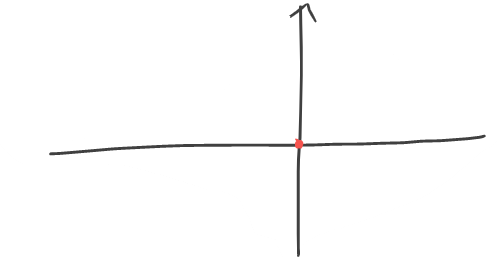
\includegraphics[width=0.5\linewidth]{figures/punkt_quadrik}
      \label{fig:punkt_quadrik}
    \end{figure}
    \item[\( \equalto{(x_1+x_2)(x_1-x_2)}{x_1^2-x_2^2}=0 \)] \tto 2 Geraden.
    \begin{figure}[H]
      \centering
      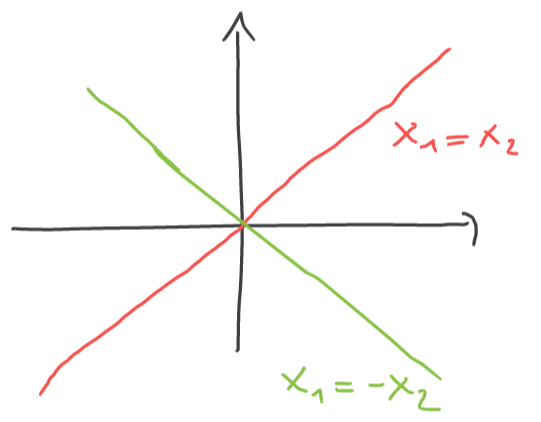
\includegraphics[width=0.5\linewidth]{figures/zwei_geraden_quadrik}
      \label{fig:zwei_geraden_quadrik}
    \end{figure}
  \end{proofdescription}
  \item \( m'=m+1 \).
  \begin{proofdescription}
    \item[\( m=0 \)] \tto \( 0=1 \)  \tto leere Menge.
    \item[\( m=1 \)] \begin{proofdescription}
      \item[\( x_1^2=1 \)]  \tto 2 parallele Geraden
      \begin{figure}[H]
        \centering
        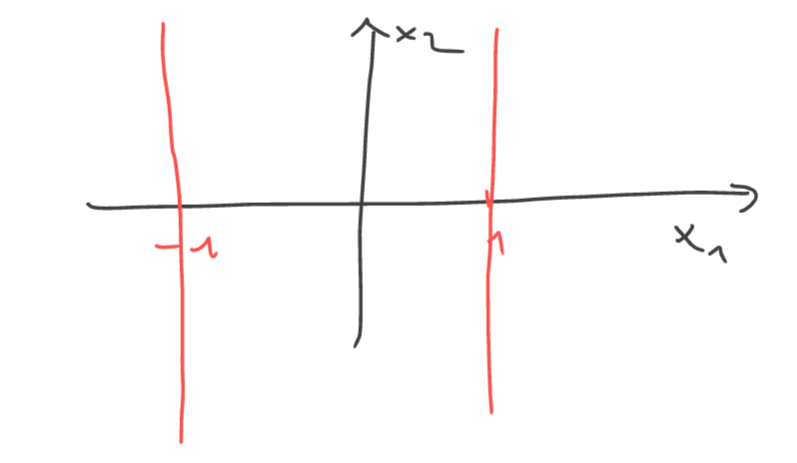
\includegraphics[width=0.5\linewidth]{figures/parallele_geraden_quadrik}
        \label{fig:parallele_geraden_quadrik}
      \end{figure}
      \item[\( -x_1^2=1 \)] \tto leere Menge.
    \end{proofdescription}
    \item[\( m=2 \)] \begin{proofdescription}
      \item[\( -x_1^2-x_2^2=1 \)] \tto \( \emptyset \).
      \item[\( x_1^2-x_2^2=1 \)] \tto Hyperbel. 
      \begin{figure}[H]
        \centering
        \includegraphics[width=0.5\linewidth]{figures/hyperbel_quadrik}
        \label{fig:hyperbel_quadrik}
      \end{figure}
      \item[\( x_1^2+x_2^2=1 \)] \tto Kreis.
      \begin{figure}[H]
        \centering
        \includegraphics[width=0.5\linewidth]{figures/ellipse_kreis_quadrik}
        \label{fig:ellipse_kreis_quadrik }
      \end{figure}
    \end{proofdescription}
    \item \( m'=m+2 \). \begin{proofdescription}
      \item[\( m=0 \)] \begin{proofdescription}
        \item[\( 2x_1=0 \)] \tto Gerade.
      \end{proofdescription}
      \item[\( m=1 \)] \begin{proofdescription}
        \item[\( x_1^2+2x_2=0 \)] \tto Parabel.
        \begin{figure}[H]
          \centering
          \includegraphics[width=0.5\linewidth]{figures/parabel_quadrik}
          \label{fig:parabel_quadrik}
        \end{figure}
      \end{proofdescription}
    \end{proofdescription}
  \end{proofdescription}
\end{eigenschaftenenumerate}
\begin{bemerkung*}
  Verschiedene dieser quadratischen Formen können als \emph{Menge} die gleiche Quadrik \( Q\subseteq \reals^2 \) beschreiben.
\end{bemerkung*}
\begin{beispiel*}
  \begin{equation*}
    \Set{(x_1,x_2)\in \reals^2|x_1^2=0}=\Set{(x_1,x_2)\subset \reals^2| 2x_1=0}.
  \end{equation*}
\end{beispiel*}
\begin{definition*}
  Wir nennen zwei Quadriken \( Q_1,Q_2\subseteq \reals^n \) \emph{geometrisch äquivalent} wenn es eine Affinität \( f\maps \reals^n\to \reals^n \) gibt mit \( f(Q_1)=Q_2 \).
\end{definition*}
\begin{frage*}
  Klassifikation aller Quadriken über \( \reals \) bis auf geometrische Äquivalenz?
\end{frage*}
Für eine Matrix \( B\in \matrices{n}{n}{\reals} \) sei \( \signature{B}=\anzahl-{} \) positive Eigenwerte von \( B \) \( -\anzahl-{} \) negative Eingenwerte von \( B \) die Signatur von \( B \).
\begin{satz}[Geometischer Klassifikationssatz (ohne Beweis)]
  Seien \( Q_1,Q_2\subset \reals^n \) nichtleere Quadriken, die beschrieben werden durch erweiterte Matrizen \( A_1',,A_2' \) mit rein quadratischen Anteilen \( A_1,A_2 \). Seien \( Q_1,Q_2 \) nicht gleich an Hyperebenen.

  Dann sind \( Q_1 \) und \( Q_2 \) \emph{geometrisch äquivalent} \gdw gilt
\begin{align*}
  \rang-{A_1}&=\rang-{A_2},\\
  \rang-{A_1'}&=\rang-{A_2'},\\
  \abs*{\signature-{A_1}}&=\abs*{\signature-{A_2}}\text{ und}\\
  \abs*{\signature-{A_1'}}&=\abs*{\signature-{A_2'}}.
\end{align*}
\end{satz}
\begin{folgerung}
  Sei \( Q\subset \reals^n \) eine nichtleere Quadrik. Dann ist \( Q \) geometrisch äquivalent zu genau einer der folgenden Quadriken.
  \begin{eigenschaftenenumerate}
    \item \label{quadriken_gleich_null_nur_quadrate}\( x_1^2+\dotsb+x_k^2-x_{k+1}^2-\dotsb-x_m^2=0 \), \( 0\leq k\leq m \), \( 2k-m\geq 0 \).
    \item \label{quadriken_gleich_eins}\( x_1^2+\dotsb+x_k^2-x_{k+1}^2-\dotsb-x_n^2=1 \), \( 1\leq k\leq m \).
    \item \label{qadriken_gleich_null_plus_ein_linearer}\( x_1^2+\dotsb+x_k^2-x_{k+1}-\dotsb-x_m^2+2x_{m+1}=0 \), \( 1\leq k\leq m \) und \( 2k-m\geq 0 \).
  \end{eigenschaftenenumerate}
\end{folgerung}
\begin{beispiele*}[Quadriken im \( \reals^3 \)]
  \begin{description}
    \item[Typ \ref{quadriken_gleich_null_nur_quadrate}] \( x_1^2+x_2^2-x_3^2=0 \)
    \begin{figure}[H]
      \centering
      \includegraphics[width=0.5\linewidth]{figures/quadriken_beispiel_kegel}
      \caption*{Kegel}
      \label{fig:quadriken_beispiel_kegel}
    \end{figure}
    \item[Typ \ref{quadriken_gleich_eins}] \begin{itemize}
      \item \( x_1^2+x_2^2=1 \).
      \begin{figure}[H]
        \centering
        \includegraphics[width=0.5\linewidth]{figures/quadriken_beispiel_kreiszylinder}
        \caption*{Kreiszylinder}
        \label{fig:quadriken_beispiel_kreiszylinder}
      \end{figure}
      \item \( x_1^2+x_2^2+x_3^2=1 \).
      \begin{figure}[H]
        \centering
        \includegraphics[width=0.5\linewidth]{figures/quadriken_beispiel_kugel}
        \caption*{Kugel}
        \label{fig:quadriken_beispiel_kugel}
      \end{figure}
      \item \( x_1^2-x_2^2+x_3^2=1 \).
      \begin{figure}[H]
        \centering
        \includegraphics[width=0.5\linewidth]{figures/quadriken_beispiel_zweischaliges_hyperboloid}
        \caption*{Zweischaliges Hyperboloid}
        \label{fig:quadriken_beispiel_zweischaliges_hyperboloid}
      \end{figure}
      \item \( x_1^2+x_2^2-x_3^2=1 \)
      \begin{figure}[H]
        \centering
        \includegraphics[width=0.5\linewidth]{figures/quadriken_beispiel_einschaliges_hyperboloid}
        \caption*{Einschaliges Hyperboloid}
        \label{fig:quadriken_beispiel_einschaliges_hyperboloid}
      \end{figure}
    \end{itemize}
    \item[Typ \ref{qadriken_gleich_null_plus_ein_linearer}] \( x_1^2+x_2^2+2x_3=0 \).
    \begin{figure}[H]
      \centering
      \includegraphics[width=0.5\linewidth]{figures/quadriken_beispiel_elliptisches_paraboloid}
      \caption*{Elliptisches Paraboloid}
      \label{fig:quadriken_beispiel_elliptisches_paraboloid}
    \end{figure}
  \end{description}
\end{beispiele*}
\file{Euklidische affine Räume}
\section{Euklidische affine Räume}
In einem allgemeinen affinen Raum \( X \) haben wir den Begriff von Gerade und parallelen Geraden (Sind \( L,L'\subset X \) Geraden, dann sagen wir, dass \( L \) und \( L' \) parallel sind, falls \( T(L)=T(L') \)).
\begin{figure}[H]
  \centering
  \includegraphics[width=0.5\linewidth]{figures/affine_geraden_lagebeziehungen}
  \label{fig:affine_geraden_lagebeziehungen}
\end{figure}
\begin{frage*}
  Können wir auch \enquote{Winkel} messen zischen zwei sich schneidenden Geraden?
\end{frage*}
\begin{erinnerung*}
  Sei \( V \) ein \( \reals \)-Vektorraum. Ein Skalarprodukt auf \( V \) ist eine \emph{positiv-definite symmetrische Bilinearform}
  \begin{equation*}
    S\maps V\times V\to \reals.
  \end{equation*}
\end{erinnerung*}
\begin{definition*}
  Ein euklidischer affiner Raum ist ein reeller affiner Raum \( (X,T(X),\tau) \) zusammen mit einem Skalarprodukt
  \begin{equation*}
    \scalarproduct{\cdot}{\cdot}\maps T(X)\times T(X)\to \reals
  \end{equation*}
  auf dem Translationsvektorraum \( T(X) \).
\end{definition*}
\begin{beispiel}
  Der \( \reals^n \) als reeller affiner Raum mit dem Standard-Skalarprodukt
  \begin{equation*}
    \begin{split}
      \scalarproduct{\cdot}{\cdot}\maps \underrelate{\vertrelation{\simeq}}{\reals^n}{T(X)}\times \underrelate{\vertrelation{\simeq}}{\reals^n}{T(X)}&\to \reals\\
      (x_1,\dotsc,x_n)\times (y_1,\dotsc,y_n)&\mapsto \sum_{i=1}^{n}x_i y_i.
    \end{split}
  \end{equation*}
\end{beispiel}
\begin{beispiel}
  Die Lösungsmenge \( L \) im \( \reals^n \) eines Systems von linearen Gleichungen \( Ax=b \), \( A\in \matrices{m }{n}{\reals} \), \( b\in \reals^m \)
  \begin{figure}[H]
    \centering
    \includegraphics[width=0.5\linewidth]{figures/hyperebene_beispiel_euklidischer_affiner_raum}
    \label{fig:hyperebene_beispiel_euklidischer_affiner_raum}
  \end{figure}
  mit dem aus dem \( \reals^n \) induzierten Standard-Skalarprodukt auf \( T(L)\explain{\text{Untervektorraum}}{\untervektorraum}\reals^n \)
  \begin{equation*}
    \scalarproduct{\cdot}{\cdot}\maps \begin{aligned}[t]
      T(L)\times T(L)&\to \reals\\
      (x,y) &\mapsto \scalarproduct{x}{y}.
    \end{aligned}
  \end{equation*}
\end{beispiel}
\begin{frage*}
  Definition von Abständen / Winkeln in einem euklidischen affinen Raum?
\end{frage*}
\begin{definition}
  Sei \( X \) ein euklidischer affiner Raum. Wir definieren eine Normabbildung
  \begin{equation*}
    \norm*{\cdot}\maps \begin{aligned}[t]
      T(X)&\to \reals_{\geq 0}\\
      t&\mapsto \norm*{t}\definedas \sqrt{\scalarproduct{t}{t}}
    \end{aligned}
  \end{equation*}
  und eine Metrik
  \begin{equation*}
    d\maps \begin{aligned}[t]
      X\times X&\to \reals_{\geq 0}\\
      (p,q)\mapsto \distance{p}{q}\definedas \norm*{\vv{pq}}.
    \end{aligned}
  \end{equation*}
  \begin{figure}[H]
    \centering
    \includegraphics[width=0.2\linewidth]{figures/metrik_auf_affinem_raum_visualisierung}
    \label{fig:metrik_auf_affinem_raum_visualisierung}
  \end{figure}
\end{definition}
\begin{bemerkung*}
  \( \norm*{\cdot} \) ist eine Norm, da \( \scalarproduct{\cdot}{\cdot} \) ein Skalarprodukt ist. Man kann nachrechnen, dass \( d \) tatsächlich eine Metrik auf \( X \) ist, \zb
  \begin{equation*}
    \distance{p}{q}=\norm*{\vv{pq}}=\norm*{-\vv{qp}}=\abs*{-1}\cdot\vv{qp}=\distance{q}{p}.
  \end{equation*}
\end{bemerkung*}
\begin{definition*}
  Sei \( X \) ein euklidischer affiner Raum, \( p,q,q'\in X \) mit \( p\neq q \), \( q' \), \( L=p\vee q \), \( L'=p\vee q' \).
  \begin{figure}[H]
    \centering
    \includegraphics[width=0.5\linewidth]{figures/affiner_winkel_definition}
    \label{fig:affiner_winkel_definition}
  \end{figure}
  Wir definieren den Winkel \( \lineangle{L}{L'} \) zwischen den Geraden \( L,L' \) durch
  \begin{equation*}
    \lineangle{L}{L'}=\arccos \frac{\abs*{\scalarproduct{\vv{pq}}{\vv{pq'}}}}{\norm*{\vv{pq}}\cdot\norm*{\vv{pq'}}}\in \interval{0}{\frac{\pi}{2}}.
  \end{equation*}
  \begin{figure}[H]
    \centering
    \includegraphics[width=0.3\linewidth]{figures/affiner_winkel_definition_wertebereich}
    \label{fig:affiner_winkel_definition_wertebereich}
  \end{figure}
  \begin{figure}[H]
    \centering
    \includegraphics[width=0.1\linewidth]{figures/affiner_winkel_definition_wertebereich_beispiel}
    \label{fig:affiner_winkel_definition_wertebereich_beispiel}
  \end{figure}
\end{definition*}
\begin{bemerkung*}
  Die Definition des Winkels \( \lineangle{L}{L'} \) ist unabhängig von der Wahl der Elemente \( q,q' \) (solange \( p\neq q,q' \)).
\end{bemerkung*}
% !TEX root = ./Vorlesungsmitschrift AGLA 2.tex  
\lecture{Di 19.05. 10:15}{}
\begin{lemma}
  Sei \( X \) ein euklidischer affiner Raum, \( t\in T(X) \) und \( \tau_t\maps X\to X \) die Translation um \( t \). Seien \( q,q'\in X \) und \( L,L'\subseteq X \) Geraden mit \( L\cap L'\neq \emptyset \). Dann gilt 
  \begin{align*}
    \distance{\tau_t(p)}{\tau_t(q)}&=\distance{p}{q}\text{ und}\\
    \lineangle{\tau_t(L)}{\tau_t(L')}&=\lineangle{L}{L'}.
  \end{align*}
\end{lemma}
\begin{proof}[Beweisidee]
  Verwende
  \begin{equation*}
    \vv{\tau_t(p) \tau_t(q)}\needed{=}\vv{pq},
  \end{equation*}
  \begin{figure}[H]
    \centering
    \includegraphics[width=0.5\linewidth]{figures/translation_erhaelt_winkel_beweis_translation_erhaelt_verschiebungen}
    \label{fig:translation_erhaelt_winkel_beweis_translation_erhaelt_verschiebungen}
  \end{figure}
  also
  \begin{equation*}
    \distance{\tau_t(p)}{\tau_t(q)}=\norm*{\vv{\tau_t(p)\tau_t(q)}}=\norm*{\vv{pq}}=\distance{p}{q}
  \end{equation*}
  für beliebige Punkte \( p,q\in X \) und \( t\in T(X) \).
  \begin{figure}[H]
    \centering
    \includegraphics[width=0.5\linewidth]{figures/translation_erhaelt_winkel_beweis_winkel_zwischen_geraden}
    \caption*{Winkel zwischen Geraden \( L,L' \)}
    \label{fig:translation_erhaelt_winkel_beweis_winkel_zwischen_geraden}
  \end{figure}
  \begin{equation*}
    \lineangle{L}{L'}=\arccos \frac{\abs{\scalarproduct{\vv{pq}}{\vv{pq'}}}}{\explain{\norm*{\vv{\tau_t(p)\tau_t(q)}}}{\norm*{\vv{pq}}}\explain[Bigg]{\norm*{\vv{\tau_t(p)\tau_t(q')}}}{\norm*{\vv{pq'}}}}.
  \end{equation*}
\end{proof}
\minisec{also:} Translation um ein Element \( t\in T(X) \) erhält Abstände und Winkel.

Nicht alle affinen Abbildungen haben diese Eigenschaft, \zb \( X=\reals^2 \) mit Standardskalarprodukt.
\begin{figure}[H]
  \centering
  \includegraphics[width=0.5\linewidth]{figures/aehnlichkeiten_gegenbeispiel}
  \caption*{\( \phi\maps X\to X \)}
  \label{fig:aehnlichkeiten_gegenbeispiel}
\end{figure}
\begin{frage*}
  Welche Abbildungen zwischen euklidischen affinen Räumen erhalten Abstände?
\end{frage*}
\begin{definition*}
  Seien \( X,X' \) metrische Räume mit Metriken \( d,d' \) und \( f\maps X\to X' \) eine Abbildung. Wir nennen \( f \) eine \emph{Isometrie}, falls \( \forall p,q\in X \) gilt
  \begin{equation*}
    d'(f(p),f(q))=\distance{p}{q}.
  \end{equation*}
\end{definition*}
\begin{frage*}
  Welche \emph{Abbildungen} zwischen euklidischen affinen Räumen erhalten Abstände?

  \tto Wir können dies Frage auf \emph{affine Abbildungen} reduzieren.
\end{frage*}
\begin{satz}\label{isometrie_affin_und_injektiv}
  Seien \( X,Y \) euklidische affine Räume \( f\maps X\to Y \) eine Isometrie. Dann ist \( f \) \emph{affin} und injektiv.
  \begin{figure}[H]
    \centering
    \includegraphics[width=0.5\linewidth]{figures/isometrie_wirklich_injektiv}
    \label{fig:isometrie_wirklich_injektiv}
  \end{figure}
\end{satz}
\begin{proof}
  Sei \( f\maps X\to X \) eine Isometrie und \( p\in X \). Betrachte die Abbildung (mit \( T(X),T(Y) \) Vektorräumen mit Skalarprodukt)
  \begin{equation*}
    F\maps \begin{aligned}[t]
      T(X)&\to T(Y)\\
      \vv{px} &\mapsto \vv{f(p)f(x)}.
    \end{aligned}
  \end{equation*}
  \begin{beweisbehauptung}
    \( F \) ist eine Isometrie.
  \end{beweisbehauptung}
  Seien \( x_1,x_2\in X \).
  \begin{align*}
    \norm*{F(\vv{px_1})-F(\vv{px_2})}_{T(Y)}&=\norm{\vv{f(p)f(x_1)}\underbrace{-\vv{f(p)f(x_2)}}_{=\vv{f(x_2)f(p)}}}_{T(Y)}\\
    &=\norm*{\vv{f(p) f(x_1)}+\vv{f(x_2) f(p)}}_{T(Y)}\\
    &=\norm*{f(x_2)f(x_1)}_{T(Y)}\\
    &=\norm*{\vv{f(x_2) f(x_1)}}_{T(Y)}\\
    &=d_Y(f(x_2), f(x_1))\\
    &\explain{\text{\( f \) ist Isometrie}}{=} d_X(x_2,x_1)=\vv{x_2 x_1}_{T(X)}\\
    &=\norm*{\vv{px_1}-\norm{\vv{px_2}}}_{T(x)}.
  \end{align*}
  \begin{beweisbehauptung}
    Ist \( F \) \emph{linear}, dann ist \( f \) affin. Seien \( x_1,x_2\in X \). Dann gilt 
    \begin{align*}
      F(\vv{x_1 x_2})&=F(\vv{x_1 p}+\vv{p x_2})\\
      &=F(-\vv{px_1}+\vv{px_2})\\
      &\explain{\text{\( F \) ist linear}}{=}-F(\vv{px_1})+F(\vv{px_2})\\
      &=-\vv{f(p)f(x_1)}+\vv{f(p) f(x_2)}\\
      &=\vv{f(x_1)f(x_2)}.
    \end{align*}
    Also ist Abbildung
    \begin{equation*}
      \vv{x_1 x_2}\mapsto \vv{f(x_1) f(x_2)}
    \end{equation*}
    linear!
  \end{beweisbehauptung}
  Es genügt also folgendes Lemma zu beweisen
  \file{Euklidische affine Räume Teil 2}
  \begin{lemma}\label{richtige_isometrie_linear}
    Seien \( V,W \) euklidisch Vektorräume, \( F\maps V\to W \) eine Isometrie mit \( F(0)=0 \). Dann ist \( F \) \emph{linear} und injektiv.
  \end{lemma}
  \begin{proof}[Beweis von Lemma~\ref{richtige_isometrie_linear}]
    \( F \) ist injektiv: Sei \( v',v\in V \) mit \( F(v)=F(v') \). Dann
    \begin{equation*}
      0=d_W(F(v),F(v'))\explain{\text{\( f \) Isometrie}}{=}d_V (v,v'),
    \end{equation*}
    also \( v=v' \).

    Zur Linearität von \( F \): \( F \) ist Isometrie, also gilt \tforall \( v_1,v_2\in V \)
    \begin{equation*}
      \underbrace{\norm*{F(v_1)-F(v_2)}_{d_W(F(v_1),F(v_2))}}=\underbrace{\norm*{v_1-v_2}}_{d_V(v_1,v_2)}.
    \end{equation*}
    Aus \( F(0)=0 \) folgt
    \begin{equation*}
      \norm*{F(v)}=\norm*{v}\quad \forall v\in V
    \end{equation*}
    Berechne für \( v_1,v_2\in V \):
    \begin{equation*}
      \norm*{v_1-v_2}^2=\scalarproduct{v_1-v_2}{v_1-v_2}=\norm*{v_1}^2+\norm*{v_2}^2-2\scalarproduct{v_1}{v_2}.
    \end{equation*}
    Es gilt auch
    \begin{equation*}
      \underbrace{\norm*{F(v_1)-F(v_2)}^2}_{\norm*{v_1-v_2}^2}=\underbrace{\norm*{F(v_1)}^2}_{\norm*{v_1}^2}+\underbrace{\norm*{F(v_2)}^2}_{\norm*{v_2}^2}-2\scalarproduct{F(v_1)}{F(v_2)}.
    \end{equation*}
    Also folgt
    \begin{equation*}
      \scalarproduct{v_1}{v_2}=\scalarproduct{F(v_1)}{F(v_2)}\quad \forall v_1,v_2\in V.
    \end{equation*}
    Seien \( v,v'\in V \).
    \begin{align*}
      \langle \underbrace{F(v+v')-F(v)-F(v')}_{\isittrue{=}0},F(v+v')-F(v)-F(v')\rangle&=\begin{aligned}[t]
        &\scalarproduct{F(v+v')}{F(v+v')}\\
        &-\scalarproduct{F(v+v')}{F(v)}\\
        &-\dotsb\\
        &+\scalarproduct{F(v')}{F(v')}
      \end{aligned}\\
      &=\begin{aligned}[t]
        &\scalarproduct{v+v'}{v+v'}\\
        &-\scalarproduct{v+v'}{v}-\dotsb\\
        &+\scalarproduct{v'}{v'}
      \end{aligned}\\
      &=\scalarproduct{v+v'-v-v'}{v+v'-v-v'} \\
      &=\scalarproduct{0}{0}=0\quad \forall v,v'\in V,
    \end{align*}
    also gilt \( F(v+v')=F(v)+F(v') \). Multiplikation mit Skalaren. Sei \( v\in V \), \( \lambda\in \reals \).
    \begin{align*}
      \scalarproduct{F(\lambda v)-\lambda F(v)}{F(\lambda v)-\lambda F(v)}&=\scalarproduct{F(\lambda v)}{F(\lambda v)}-2\scalarproduct{F(\lambda v)}{\lambda F(v)}\scalarproduct{\lambda F(v)}{\lambda F(V)}\\
      &=\scalarproduct{F(\lambda v)}{F(\lambda v)}-2\lambda \scalarproduct{F(\lambda v)}{F(v)}+\lambda^2\scalarproduct{F(v)}{F(v)}\\
      &=\scalarproduct{\lambda v}{\lambda v}-2\lambda \scalarproduct{\lambda v}{v}+\lambda^2\scalarproduct{v}{v}=(\lambda^2-2\lambda^2+\lambda^2)\scalarproduct{v}{v}\\
      &=0,
    \end{align*}
    also \( F(\lambda v)=\lambda F(v)\quad  \forall \forall \lambda\in\reals\logicspace \forall v\in V \).
  \end{proof}
\end{proof}
\file{Kongruenz}
\begin{definition*}
  Eine Isometrie \( f\maps X\to X \) eines euklidischen affinen Raumes \( X \) nennen wir \emph{Kongruenz} (also nach \thref{isometrie_affin_und_injektiv} immer eine Affinität).
\end{definition*}
\begin{lemma}
  Sei \( f\maps X\to X \) eine Affinität eines euklidischen affinen Raumes \( X \). Dann ist \( f \) eine \emph{Kongruenz} genau dann, wenn die zugehörige lineare Abbildung \( F\maps T(X)\to T(X) \) \emph{orthogonal} ist.
\end{lemma}
\begin{proof}
  \( f  \) ist Isometrie \gdw
  \begin{equation*}
    \distance{f(p)}{f(q)}=\distance{p}{q}\quad \forall p,q\in X,
  \end{equation*}
  \dh \gdw
  \begin{equation*}
    \equalto{\norm*{F(\vv{pq})}}{\norm*{f(p)f(q)}}=\norm{\underbrace{\vv{pq}}_{\in T(X)}} \quad \forall p,q\in X.
  \end{equation*}
  Dies ist äquivalent dazu, dass \( F \) orthogonal ist (also das Skalarprodukt erhält)
\end{proof}
\file{Ähnlichkeiten}
\begin{bemerkung*}
  Im \( \reals^n \) mit Standardskalarprodukt sind Kongruenzen
  \begin{equation*}
    f\maps \reals^n\to \reals^n
  \end{equation*}
  genau durch die Abbildungen der Form
  \begin{equation*}
    f\maps x\mapsto \boxed{f(0)*A\matrixmult x}\quad \forall x\in \reals^n
  \end{equation*}
  gegeben mit \( A\in \orthogonalmatrices{n}{\reals} \) orthogonal, \dh \( \inverse-{A}=\transpose-{A} \). Slogan: \enquote{Kongruenz \( \sim \) orthogonale Abbildung + Translation}.
\end{bemerkung*}
\begin{frage*}
  Kongruenzen erhalten Winkel. Welche \emph{Affinitäten}/ Abbildungen \( f\maps X\to X \) eines euklidischen Raumes \( X \) haben diese Eigenschaft?
\end{frage*}
\begin{beispiel*}
  \( \reals^2 \) mit Standardskalarprodukt.
  \begin{figure}[H]
    \centering
    \includegraphics[width=0.5\linewidth]{haus_zu_haus}
    \label{fig:haus_zu_haus}
  \end{figure}
  erhält Winkel, aber nicht Abstände, \dh ist keine Isometrie des \( \reals^2 \).
\end{beispiel*}
\begin{definition*}
  Sei \( X \) ein euklidischer affiner Raum, \( f\maps X\to X \) eine Abbildung. Sei \( \rho\in \reals_{>0} \). Wir nennen \( f  \) eine \emph{Ähnlichkeit} mit (Ähnlichkeits-) Faktor \( \rho \) wenn \tforall  \( p,q\in X \) gilt
  \begin{equation*}
    \distance{f(p)}{f(q)}=\rho\cdot \distance{p}{q}.
  \end{equation*}
\end{definition*}
\begin{korollar*}[aus \thref{isometrie_affin_und_injektiv}]
  Eine Ähnlichkeit \( f\maps X\to X \) eines euklidischen affinen Raumes \( X \) ist eine Affinität.
\end{korollar*}
\begin{proof}
  Sei \( p_0\in X \). Wir definieren eine Affinität
  \begin{equation*}
    \inv{\rho}\maps X\to X
  \end{equation*}
  durch \( \inv{\rho}(p_0)=p_0 \) und
  \begin{equation*}
    \tilde{\rho}\maps \begin{aligned}[t]
      T(X)&\to T(X)\\
      T(X)\ni v&\mapsto \inv{\rho}v.
    \end{aligned}
  \end{equation*}
  \begin{figure}[H]
    \centering
    \includegraphics[width=0.5\linewidth]{figures/aehnlichkeiten_sind_affinitaeten_beweis}
    \label{fig:aehnlichkeiten_sind_affinitaeten_beweis}
  \end{figure}
  Wir betrachten die Abbildung
  \begin{equation*}
    \inv{\rho}\circ f\maps X\to X.
  \end{equation*}
  \begin{behauptung*}
    \( \inv{\rho}\circ f \) ist eine Isometrie.
  \end{behauptung*}
  Seien \( p,q\in X \). Dann gilt
  \begin{equation*}
    \distance{\inv{\rho}\circ f(p)}{\inv{\rho}(f(q))}=\norm{\vv{\inv{\rho}\circ f(p) \inv{\rho}\circ f(q)}}
  \end{equation*}
  also
  \begin{align*}
    \distance{\inv{\rho}\circ f(p)}{\inv{\rho}(f(q))}&=\norm*{\inv{\rho}\vv{f(p)f(q)}}\\
    &=\inv{\rho}\norm*{\vv{f(p)f(q)}}\\
    &\explain{\text{\( f \) ist Ähnlichkeit mit Faktor \( \rho \)}}{=}\distance{p}{q},
  \end{align*}
  also ist nach \thref{isometrie_affin_und_injektiv} \( \inv{\rho}\circ f \) injektiv und affin. Damit ist auch \( f \) Affinität.
\end{proof}
% !TEX root = ./Vorlesungsmitschrift AGLA 2.tex  
\lecture{Fr 21.05. 10:15}{}
Eine Weitere Eignenschaft von Ähnlichkeiten:
\begin{satz}
  Sei \( X \) ein euklidischer affiner Raum und \( f\maps X\to X \) eine Ähnlichkeit mit Ähnlichkeitsfaktor \( \rho\neq 1 \). Dann besitzt \( f \) genau einen Fixpunkt.
\end{satz}
\begin{proof}[Beweisidee]
  Nach obigem Korollar ist \( f \) eine Affinität. Sei \( F\maps T(X)\to T(X) \) die zugehörige lineare Abbildung. Dann ist \( \frac{1}{\rho} F \) orthogonal, also haben alle Eigenwerte von \( F \) Betrag \( \rho \). 

  Nach Wahl eines Koordinatensystem wird \( f \) beschrieben durch
  \begin{align*}
    \reals^n&\to \reals^n\\
    x&\mapsto \braceannotate{\isittrue{=}x}{Ax+b}.
  \end{align*}
  mit \( A\in \sqmatrices{n}{\reals} \), \( k\subset \reals^n \) und Fixpunkten beschrieben durch
  \begin{equation*}
    Ax+b=x,
  \end{equation*}
  also \( (A-I_n)x=-b \), da \( 1 \) kin Eigenwert von \( A \) ist, gilt \( \det(A-I_n)\neq 0 \).
\end{proof}
Ähnlichkeiten erhalten Winkel. Gibt es noch weitere Affinitäten eines euklidischen affinen Raumes, die Winkel erhalten?
\begin{definition*}
  Sei \( X \) ein euklidischer affiner Raum, \( L,L'\subseteq X \) Geraden mit \( L\cap L'\neq \emptyset \). Wir nennen \( L \) und \( L' \) orthogonal, wenn gilt
  \begin{equation*}
    \lineangle{L}{L'}=\frac{\pi}{2}.
  \end{equation*}
  Schriebe auch \( L\perp L' \).
\end{definition*}
\begin{satz}\label{nur_aehnlichkeiten_erhalten_rechte_winkel}
  Sei \( X \) ein euklidischer affiner Raum und \( f\maps X\to X \) eine Affinität mit der Eigenschaft, dass für alle Geraden \( L,L' \) mit \( L\cap L'\neq \emptyset \) und \( L\perp L' \) gilt, dass
  \begin{equation*}
    f(L)\perp f(L').
  \end{equation*}
  Dann ist \( F \) eine Ähnlichkeit.
  \begin{figure}[H]
    \centering
    \includegraphics[width=0.5\linewidth]{figures/rechte_winkel_erhalten}
    \label{fig:rechte_winkel_erhalten}
  \end{figure}
\end{satz}
\begin{proof}
  Sei \( F\maps T(X)\to T(X) \) die zugehörige bijektive lineare Abbildung. Seien \( p,q,q'\in X \) mit \( p\vee q=L \), \( p\vee q'=L' \) und \( L\perp L' \). Dann gilt \( \lineangle{L}{L'}=\frac{\pi}{2} \), also
  \begin{equation*}
    \arccos \frac{\abs{\scalarproduct{\vv{pq}}{\vv{pq'}}}}{\norm{\vv{pq}}\norm{\vv{pq}}}=\frac{\pi}{2}
  \end{equation*}
  \dh \( \scalarproduct{\vv{pq}}{\vv{pq'}}=0 \).
  \begin{figure}[H]
    \centering
    \includegraphics[width=0.5\linewidth]{figures/rechte_winkel_skalarprodukt}
    \label{fig:rechte_winkel_skalarprodukt}
  \end{figure}
  Die Geraden \( f(L) \) und \( f(L') \) sind gegeben durch
  \begin{equation*}
    f(p)\vee f(q)=f(L)\qquad f(p)\vee f(q')=f(L')
  \end{equation*}
  und wir können annehmen (wegen \( f(L)\perp f(L') \)), dass 
  \begin{equation*}
    \braceannotate{\scalarproduct{F(\underrelate{\vertni}{T(X)}{\underbrace{\vv{pq}}})}{F(\underrelate{\vertni}{T(X)}{\underbrace{\vv{pq'}}})}}{\scalarproduct{\vv{f(p)f(q)}}{f(p)f(q')}}=0.
  \end{equation*}
Es gilt also, dass für alle \( v,w\in T(X) \) mit \( \scalarproduct{v}{w}=0 \) gilt \( \scalarproduct{F(v)}{F(w)}=0 \). Wir haben den Beweis von \thref{nur_aehnlichkeiten_erhalten_rechte_winkel} auf folgendes Lemma reduziert.
\end{proof}
\begin{lemma}
  Sei \( V \) ein euklidischer Vektorraum, \( F\maps V\to V  \) ein Isomorphismus mit \( F(v)\perp F(w) \) für alle \( v,w\in V \) mit \( v\perp w \). Dann existiert \( \rho\in \reals_{>0} \) \sd \( \frac{1}{\rho}\cdot F \) orthogonal ist.
\end{lemma}
\begin{proof}
  Sei \( n=\dim V \) und \( v_1,\dotsc, v_n \) eine Orthonormal von \( V \), \dh \( \norm{v_i}=1 \), \( 1\leq i\leq n \) und \( \scalarproduct{v_i}{v_\gamma}=0 \) für \( i\leq j \). Sei \( \rho_i\definedas \norm{F(v_i)}  \), \( 1\leq i \leq n \).
  \begin{figure}[H]
    \centering
    \includegraphics[width=0.5\linewidth]{figures/orthonormalbasis_skalierung}
    \label{fig:orthonormalbasis_skalierung}
  \end{figure}
  Fpr \( j\neq j \) gilt 
  \begin{equation*}
    \scalarproduct{v_i+v_j}{v_i-v_j}=\braceannotate{\norm{v_i}^2}{=1}+\braceannotate{\scalarproduct{v_j}{v_i}}{=0}-\braceannotate{\scalarproduct{v_i}{v_j}}{=0}-\braceannotate{\norm{v_j}^2}{=1}=0, 
  \end{equation*}
  also \( v_i+v_j\perp v_i-v_j \). Nach Annahme gilt dann auch
  \begin{equation*}
    \scalarproduct{F(v_i)}{F(v_i)}+\braceannotate{\scalarproduct{F(v_j)}{F(v_i)}}{=0, \text{ da } F(v_j)\perp F(v_i)}-\braceannotate{\scalarproduct{F(v_i)}{F(v_j)}}{=0}-\scalarproduct{F(v_j)}{F(v_j)}=\scalarproduct{F(v_i+v_j)}{F(v_i-v_j)}=0.
  \end{equation*}
  Also gilt
  \begin{equation*}
    \equalto{\rho_i^2}{\norm{F(v_i)}^2}=\equalto{\rho_j^2}{\norm{F(v_j)}^2} \quad \forall i,j
  \end{equation*}
  und damit \( \rho_i=\rho_j \quad \forall 1\leq i,j\leq n \). Schreibe \( \rho=\rho_i \quad \forall 1\leq i \leq n \) für den gemeinsamen Wert. Dann ist die Abbildung \( \frac{1}{\rho}F \) orthogonal, da \( v_1,\dotsc, v_n \) auf die Orthonormalbasis \( \frac{1}{\rho}F(v_1),\dotsc,\frac{1}{\rho}F(v_n) \) abgebildet wird.
\end{proof}
Sei \( f\maps \reals^n\to \reals^n \) eine Affinität gegeben durch 
\begin{equation*}
  x\mapsto Ax+b\qquad A\in \invertiblematrices{n}{\reals}\quad b\in \reals^n.
\end{equation*}
Im Obigen haben wir gesehen, dass gilt: \( f \) ist \emph{Kongruenz} \tiff \( A \) ist \emph{orthogonal}, \( f \) ist Ähnlichkeit \( \frac{1}{\rho}A \) ist orthogonal für ein \( \rho\geq 0 \).
\begin{frage*}
  Wie können wir \( A\in \invertiblematrices{n}{\reals} \) für eine allgemeine Affinität \( f \) mit Hilfe von / bis auf eine orthogonale Matrix möglichst einfach ausdrücken?
\end{frage*}
Betrachte \( \reals^n \) als euklidischen affinen Raum mit Standard-skalarprodukt
\begin{gather*}
  \scalarproduct{\cdot}{\cdot}\maps \begin{aligned}[t]
    \reals^n\times\reals^n &\to \reals_{\geq 0}\\
    (x_1,\dotsc,x_n)\times(y_1,\dotsc,y_n)&\mapsto \sum_{i=1}^{n}x_i y_i.
  \end{aligned}
\end{gather*}
\begin{satz}[Hauptachsentransformation von Affinitäten]\label{hauptachsentransformation_affinitaeten}
  Sei \( f\maps \reals^n\to \reals^n \) eine Affinität gegeben durch \( x\mapsto Ax+b \) mit \( A\in \invertiblematrices{n}{\reals} \), \( b\in \reals^n \). Dann gibt es orthogonale Matrizen \( S,T\in \orthogonalmatrices{n} \) und eine Diagonalmatrix
  \begin{equation*}
    D=\begin{pNiceMatrix}
      \alpha_1 &  & \Block{2-2}<\large>{0} & \\
       & \alpha_2 & & \\
      \Block{2-2}<\large>{0} &  & \Ddots \\
       &  & & \alpha_n
    \end{pNiceMatrix}
  \end{equation*}
  mit \( \alpha_1,\dotsc,\alpha_n>0 \), \sd
  \begin{equation*}
    A=SDT
  \end{equation*}
  \dh
  \begin{equation*}
    f(x)=SDTx+f(0).
  \end{equation*}
\end{satz}
\begin{proof}
  Wir bilden die Matrix \( C=\transpose{A}A \).
  \begin{itemize}
    \item \( C \) ist symmetrisch da
    \begin{equation*}
      \transpose{C}=\transpose{(\transpose{A}A)}=\transpose{A}\transpose{\transpose{A}}=\transpose{A}A=C.
    \end{equation*}
    \item \( C \) ist positiv definit, denn \( I_n \) ist positiv definit und daher nach dem Sylvesterschen Trägheitsgesetz auch \( C \). Aus der Hauptachsentransformation symmetrischer Matrizen (\agla{1}) folgt, dass es eine Matrix \( T\in \orthogonalmatrices{n} \) mit
    \begin{equation*}
      TC\transpose{T}=\begin{pNiceMatrix}
        \beta_1 &  & 0 \\
         & \Ddots &  \\
        0 &  & \beta_n
      \end{pNiceMatrix},
    \end{equation*}
    \( \beta_1,\dotsc,\beta_n>0 \). Wir definieren \( \alpha_i=\sqrt{\beta_i} \), \( 1\leq i\leq n \) und 
    \begin{equation*}
      D\definedas \begin{pNiceMatrix} \alpha_1 &  &  \\  & \Ddots &  \\  &  & \alpha_n \end{pNiceMatrix},
    \end{equation*}
    Dann gilt
    \begin{equation*}
      T\braceannotate{\transpose{A}A}{\transpose{C}}\transpose{T}=D^2=\transpose{D}D,
    \end{equation*}
    also
    \begin{equation*}
      I_n=\braceannotate{S}{\inv{\transpose{A}}\transpose{T}\transpose{D}}\braceannotate{\transpose{S}}{DT\inv{A}}.
    \end{equation*}
    Sei \( S\definedas \inv{\transpose{A}}\transpose{T}\transpose{D} \). Dann gilt \( \transpose{S}S=I_n \) und \( S\in \orthogonalmatrices{n} \) ist orthogonal. Wir erhalten \( \transpose{S}=DT\inv{A} \) und \( A=SDT \).
  \end{itemize}
\end{proof}
\begin{korollar*}
  Sei \( f\maps \reals^n\to \reals^n \) ein Isomorphismus des Vektorraumes \( \reals^n \). Dann gibt es eine Orthonormalbasis \( v_1,\dotsc, v_n\in \reals^n \), \sd die Vektoren \( F(v_1),\dotsc,F(v_n) \) eine Orthogonalbasis bilden.
\end{korollar*}
\begin{proof}
  Sei \( F \) bezüglich der Standardbasis der \( \reals^n \) gegeben durch die Matrix \( A\in \invertiblematrices{n}{\reals} \). Aus \thref{hauptachsentransformation_affinitaeten} folgt, dass es orthogonale Matrizen \( S,T\in \orthogonalmatrices{n} \) gibt mit \( A=SDT \) und
  \begin{equation*}
    D=\begin{pNiceMatrix}
      \alpha_1 &  & 0 \\
       & \Ddots &  \\
      0 &  & \alpha_n
    \end{pNiceMatrix},
  \end{equation*}
  \( \alpha_1,\dotsc,\alpha_n>0 \) einer Diagonalmatrix. Sei \( v_i=\transpose{T}e_i \), \( 1\leq i\leq n \). \( T \) ist orthogonal, also auch \( \transpose{T} \) und damit ist \( v_1,\dotsc,v_n \) eine Orthonormalbasis des \( \reals^n \). Es gilt
  \begin{align*}
    F(v_i)&=A\transpose{T}e_i\\
    &=SD\braceannotate{T\transpose{T}}{I_n}e_i\\
    &=SDe=S(\alpha_i e_i)\\
    &=\alpha_i S_{e_i}.
  \end{align*}
  Die Matrix \( S \) ist orthogonal, also sind die Vektoren \( Se_1,\dotsc,Se_n \) eine Orthonormalbasis. Da \( \alpha_1,\dotsc,\alpha_n>0 \), bilden \( F(v_1),\dotsc,F(v_n) \) eine orthogonal Basis der \( \reals^n \).
\end{proof}
\begin{beispiel*}
  \phantom{Ein Beispiel}
  \begin{figure}[H]
    \centering
    \includegraphics[width=0.5\linewidth]{figures/orthonormalbasis_auf_orthogonalbasis}
    \label{fig:orthonormalbasis_auf_orthogonalbasis}
  \end{figure}
\end{beispiel*}
% !TEX root = ./Vorlesungsmitschrift AGLA 2.tex  
\chapter{Projektive Geometrie}
\section{Projektive Räume}
\file{Projektive Räume}
\lecture{Di 26.05. 10:15}{}

Sei \( K \) ein Körper und 
\begin{equation*}
  P(x_1,\dotsc, x_n)\in \polynomials{K}{x_1,\dotsc,x_n}
\end{equation*}
ein quadratisches Polynom der Form 
\begin{equation*}
  P(x_1,\dotsc,x_n)=\sum_{1\leq i\leq j \leq n}\alpha_{ij}x_i x_j
\end{equation*}
it \( \alpha_{ij}\in K \), \( 1\leq i \leq j\leq n \). Sei
\begin{equation*}
  Q=\Set{(x_1,\dotsc,x_n)\in K^n|P(x_1,\dotsc,x_n)=0}
\end{equation*}
die durch \( P \) beschriebene Quadrik.

Sei \( \lambda\in \star{*} \). Dann gilt für \( (x_1,\dotsc,x_n)\in K^n \)
\begin{equation*}
  (x_1,\dotsc,x_n)\in Q\iff \lambda(x_1,\dotsc,x_n)\in Q.
\end{equation*}
Denn \( P(x_1,\dotsc,x_n)=0 \) ist äquivalent zu 
\begin{equation*}
  0=\lambda^2 P(x_1,\dotsc,x_n)=\lambda^2 \sum_{\mathclap{1\leq i\leq j\leq n}} \alpha_{ij}x_i x_j=\sum_{\mathclap{1\leq i\leq j\leq n}} \alpha_{ij}(\lambda x_i)(\lambda x_j)=P(\lambda(x_1,\dotsc,x_n)).
\end{equation*}
Mit \( (x_1,\dotsc,x_n)\in Q \) ist also auch
\begin{equation*}
  \braceannotate{\mathclap{\Set{\lambda\cdot (x_1,\dotsc,x_n)|\lambda\in K}}}{K\cdot (x_1,\dotsc, x_n)}\subseteq Q
\end{equation*}
\dh \( Q \) \enquote{besteht aus einer Vereinigung an Geraden}.
\begin{idee*}
  Im projektiven Raum identifizieren wir die Punkte der Gerade \( K\cdot(x_1,\dotsc,x_n) \) zu einem Punkt.
\end{idee*}  
\begin{definition*}
  Sei \( K \) ein Körper und \( V \) ein \( K \)-Vektorraum. Wir definieren
  \begin{equation*}
    \projectionspace{V}=\Set{L\untervektorraum V| L\ \text{ist eindimensionaler Untervektorraum von \( V \)}}.
  \end{equation*}
\end{definition*}
\begin{beispiel*}
  \( V=\reals^2 \) als \( \reals \)-Vektorraum.
  \begin{figure}[H]
    \centering
    \includegraphics[width=0.5\linewidth]{projektion_r_2_beispiel}
    \caption*{\( \projectivedim{\projectionspace{V}}=1 \).}
    \label{fig:projektion_r_2_beispiel}
  \end{figure}
\end{beispiel*}
\begin{bemerkung*}
  Für \( V=\zeroset \) erhalte
  \begin{equation*}
    \projectivedim{\projectionspace{V}}=\dim{K}{V}-1=0-1=-1
  \end{equation*}
  und \( \projectionspace{V}=\emptyset \).
\end{bemerkung*}
\begin{bspdef}
  Sei \( K \) ein Körper, \( n\geq 0 \). Dann ist \( \projectionspace{K^{n+1}} \) die Menge der Geraden durch den Ursprung im \( K^{n+1} \). Wir bezeichnen
  \begin{equation*}
    \projectionspaceover{n}{K}\definedas \projectionspace{K^{n+1}}
  \end{equation*}
  als \( n \)-dimensionalen projektiven Raum über \( K \). Weiter definieren wir die projektive Dimension von \( \projectionspace{V} \) als \( \projectivedim{\projectionspace{V}}\definedas \dim{K}{V}-1 \).
\end{bspdef}
\begin{bemerkung*}
  Für einen \( K \)-Vektorraum \( V \) haben wir immer eine Abbildung
  \begin{equation*}
    \begin{split}
      V\setminus\zeroset &\to \projectionspace{V}\\
      v&\mapsto K\cdot v.
    \end{split}
  \end{equation*}
  \begin{figure}[H]
    \centering
    \includegraphics[width=0.5\linewidth]{einfachste_projektion}
    \caption*{\textcolor{Cyan}{\( \projectionspace{\reals^2}\text{\enquote{\( \sim \)}}\reals^1\cup \Set{\infty} \)}}
    \label{fig:einfachste_projektion}
  \end{figure}
\end{bemerkung*}
\begin{definition*}[homogene Koordinaten]
  \( n\in \wholes_{\geq 0} \). Sei \( K \) ein Körper und \( L\in \projectionspaceover{n}{K} \). Wir nennen ein Tupel
  \begin{equation*}
    (x_0,\dots,x_n)\in K^{n+1}\setminus\zeroset
  \end{equation*}
  homogene Koordinaten des Punktes \( L\in \projectionspaceover{n}{K} \), falls 
  \begin{equation*}
    K\cdot (x_0,\dotsc,x_n)=L.
  \end{equation*}
  Schreibe auch
  \begin{equation*}
    (x_0:\dotsc:x_n)\definedas K\cdot(x_0,\dotsc,x_n).
  \end{equation*}
\end{definition*}
\begin{bemerkung*}
  Die homogenen Koordinaten eines Punktes \( L\in \projectionspaceover{n}{K} \) sind nur bis auf Multiplikation mit \( \lambda\in \fieldwithoutzero{K} \) eindeutig bestimmt, \dh für \( (x_0,\dotsc,x_n),(y_0,\dotsc,y_n)\in K^{n+1}\setminus \zeroset \) gilt
  \begin{equation*}
    (x_0:\dotsc:x_n)=(y_0:\dotsc:y_n)
  \end{equation*}
  \gdw
  \begin{equation*}
    K(x_0,\dotsc,x_n)=K(y_0,\dotsc,y_n),
  \end{equation*}
  \dh wenn \texists  \( \lambda\in \fieldwithoutzero{K} \) mit
  \begin{equation*}
    (x_0,\dotsc,x_n)=\lambda (y_0,\dotsc,y_n).
  \end{equation*}
\end{bemerkung*}
\subsection*{Unterräume eines projektiven Raums}
\begin{beispiel}\label{projektive_unterebene}
  \( V=\reals^3 \), die Menge der Geraden \( \reals\cdot(0,v_1,v_2) \) mit \( (v_1,v_2)\in \reals^2\setminus\zeroset \) \enquote{sieht genauso aus} wie
  \begin{equation*}
    \projectionspaceover{1}{\reals}=\projectionspace{\reals^2}.
  \end{equation*}
  Wir wollen
  \begin{equation*}
    \Set{\reals\cdot (0,v_1,v_2)|(v_1,v_2)\in \reals^2\setminus\zeroset\subseteq \projectionspace{\reals^3}}
  \end{equation*}
  als projektiven Unterraum erklären.
  \begin{figure}[H]
    \centering
    \includegraphics[width=0.5\linewidth]{projektiver_unterraum_beispiel}
    \label{fig:projektiver_unterraum_beispiel}
  \end{figure}
\end{beispiel}
\begin{definition*}
  Sei \( V \) ein \( K \)-Vektorraum und \( Z\subseteq \projectionspace{V} \). Wir nennen \( Z \) einen projektiven Unterraum von \( \projectionspace{V} \), falls es einen \( K \)-Untervektorraum \( W\untervektorraum V \) gibt mit \( Z=\projectionspace{W} \). Wir nennen \( Z\subseteq \projectionspace{V} \) eine
  \begin{itemize}
    \item (projektive) Gerade, wenn \( \projectivedim-{Z}=1 \),
    \item (projektive) Ebene, wenn  \( \projectivedim-{Z}=2 \),
    \item (projektive) Hyperebene, wenn \( \projectivedim-{Z}=\projectivedim{\projectionspace{V}}-1 \).
  \end{itemize}
\end{definition*}
\begin{bemerkung*}
  Ist \( Z\subseteq \projectionspace{V} \) ein projektiver Unterraum mit \( Z=\projectionspace{W} \) für einen Untervektorraum \( W\untervektorraum V\), so ist
  \begin{equation*}
    W=\bigcup_{p\in Z} p
  \end{equation*}
  Vereinigung von Geraden in \( Z \).
\end{bemerkung*}
Zurück zum obigen Beispiel: \( V=\reals^3 \), \( W=\Set{(0,x_1,x_2)|x_1,x_2\in\reals^3}\simeqq \reals^2 \). Dann ist \( Z=\projectionspace{W}\subseteq \projectionspace{V} \) ein projektiver Unterraum. Was bleibt übrig, wenn wir \( \projectionspace{\reals^3}\setminus\projectionspace{W} \) betrachten?
\begin{figure}[H]
  \centering
  \includegraphics[width=0.5\linewidth]{ohne_projektiven_unterraum_r_2_beispiel}
  \label{fig:ohne_projektiven_unterraum_r_2_beispiel}
\end{figure}
\( \projectionspace{W} \): Geraden, die in der \( x_1 \)-\( x_2 \)-Ebene enthalten sind. Betrachte die affine Ebene
\begin{equation*}
  E=\Set{(1,x_1,x_2)|x_1,x_2\in \reals^2}\subseteq \reals^3.
\end{equation*}
Sei \( L\in \projectionspace{V}\setminus \projectionspace{W} \). Dann gibt es genau einen Schnittpunkt \( L\cap E \). Die Abbildung
\begin{equation*}
  \begin{split}
    \projectionspace{V}\setminus\projectionspace{W}&\to E\explain{\text{als affiner Raum über \( \reals \)}}{\simeqq}\reals^2\\
    L&\mapsto L\cap E
  \end{split}
\end{equation*}
ist bijektiv.

\minisec{Allgemein:} Sei \( K \) ein Körper und betrachte im \( K^{n+1} \) den Untervektorraum
\begin{equation*}
  W\definedas \Set{(x_0,\dotsc,x_n)\in K^{n+1}|x_0=0}.
\end{equation*}
Dann ist \( H\definedas \projectionspace{W}\subseteq \projectionspaceover{n}{K} \) eine (projektive) Hyperebene. Falls 
\begin{equation*}
  (y_0:\dotsc:y_n)\in \projectionspaceover{n}{K}\setminus H,
\end{equation*}
dann ist \( y_0\neq 0 \), also ist 
\begin{equation*}
  (y_0:\dotsc:y_n)=\left( 1:\frac{y_1}{y_0}:\dotsc:\frac{y_n}{y_0} \right)
\end{equation*}
von der Form \( (1:x_1:\dotsc:x_n) \) mit \( x_1,\dotsc,x_n \in K\). Zwei Tupel \( (x_1,\dotsc,x_n)\neq(x_1',\dotsc,x_n')\in K^n \) induzieren unterschiedliche Projektive Punkte im \( \projectionspaceover{n}{K} \).
\begin{equation*}
  (1:x_1:\dotsc:x_n)\neq (1:x_1':\dotsc:x_n')\in \projectionspaceover{n}{K}.
\end{equation*}
Aus
\begin{equation*}
  (1,x_1,\dotsc,x_n)=\lambda(1,x_1',\dotsc,x_n')
\end{equation*}
folgt \( \lambda=1 \).

Wir erhalten eine Bijektion
\begin{equation*}
  \begin{split}
    \phi\maps K^n&\to \projectionspaceover{n}{K}\setminus H\\
    (x_1,\dotsc,x_n)&\mapsto (1:x_1:\dotsc:x_n)
  \end{split}
\end{equation*}
und damit eine Einbettung
\begin{equation*}
  \begin{split}
    \iota\maps K^n&\to \projectionspaceover{n}{K}\\
    (x_1,\dotsc,x_n)&\mapsto (1:x_1:\dotsc:x_n),
  \end{split}
\end{equation*}
die wir kanonische Einbettung des \( K^n \) in den \( \projectionspaceover{n}{K} \) nennen.

\subsection*{Dimensionsformel als nächstes Ziel}
\begin{lemma}\label{schnitt_von_projektiven_unterraeumen_ist_projektiver_unterraum}
  Sei \( V \) ein \( K \)-Vektorraum und \( (Z_i)_{i\in I} \) eine Familie projektiver Unterräume von \( \projectionspace{V} \), \( i\in I \) gibt es eine Familie projektiver Unterräume von \( \projectionspace{V} \). Dann ist \( \bigcap_{i\in I} Z_i \) in projektiver Unterraum von \( \projectionspace{V} \).
\end{lemma}
\begin{proof}
  Zu jedem \( Z_i\subseteq \projectionspace{V} \), \( i\in I \), gibt es einen \( K \)-Untervektorraum \( W_i\subseteq V \) mit \( Z_i=\projectionspace{W_i} \). Es gilt
  \begin{equation*}
    \begin{split}
      \bigcap_{i\in I}Z_i&=\bigcap_{i\in I}\Set{L\subseteq V|\text{Gerade mit \( L\subseteq W_i \)}}\\
      &=\bigcap_{i\in I}\Set{L\subseteq V|\text{Gerade \( L \) mit \( L\subseteq  \smash{\underbrace{\bigcap_{i\in I}W_i}_{\mathclap{\text{\( K \)-Untervektorraum}}}\vphantom{\bigcup_{i\in I}}}\)}}\\
      &=\projectionspace*{\bigcap_{i\in I} W_i}
    \end{split}
  \end{equation*}
\end{proof}
\addtocounter{beispiel}{-1}
\begin{beispiel}
  \( V=\reals^3 \), also \( \projectionspace{V}=\projectionspaceover{2}{\reals} \) die projektive Ebene über \( \reals \).
  \begin{equation*}
    \begin{split}
      \iota\maps \reals^2&\to \projectionspaceover{2}{\reals}\\
      (x_1,x_2)&\mapsto (1:x_1:x_2)
    \end{split}
  \end{equation*}
  kanonische Einbettung. Betrachte die projektiven Geraden
  \begin{equation*}
    Z_1=\Set{(x_0:x_1:x_2)\in \projectionspaceover{2}{\reals}|x_1=0}=\projectionspace{W_1}
  \end{equation*}
  mit
  \begin{equation*}
    W_1=\Set{(x_0,x_1,x_2)\in\reals^3|x_1=0}
  \end{equation*}
  und \( Z_2=\projectionspace{W_2} \) it
  \begin{equation*}
    W_2=\Set{(x_0,x_1,x_2)\in \reals^3|x_0=x_1}.
  \end{equation*}
  Seien \( Y_1,Y_2\subseteq \reals^2 \) die affinen Geraden gegeben durch
  \begin{align*}
    Y_1&=\Set{(x_1,x_2)\in\reals^2|x_1=0}\\
    Y_2&=\Set{(x_1,x_2)\in \reals^2|x_1=1}.
  \end{align*}
  Dann ist \( Z_1=\iota(Y_1)\cup \Set{(0:0:1)} \) und \( Z_2=\iota(Y_2)\cup \Set{(0:0:1)} \). Es ist \( Y_1\cap Y_2=\emptyset \). (\( Y_1,Y_2 \) sind parallele Geraden), aber \( Z_1\cap Z_2=\Set{(0:0:1)} \). \enquote{Wir sagen auch, die Geraden \( Z_1,Z_2 \) schneiden sich in dem unendlich fernen Punkt \( (0:0:1) \)}.
  \begin{figure}[H]
    \centering
    \includegraphics[width=0.5\linewidth]{schnitt_projektiver_geraden_r_3_beispiel}
    \label{fig:schnitt_projektiver_geraden_r_3_beispiel}
  \end{figure}
\end{beispiel}
\begin{bemerkung*}
  Die Vereinigung von projektiven Unterräumen eines projektiven Raumes \( \projectivedim{V} \) ist im Allgemeinen selbst kein projektiver Unterraum.
\end{bemerkung*}
\begin{frage*}
  Seien \( Z_i \), \( i\in I \) projektive Unterräume von \( \projectionspace{V} \). Finde den kleinsten projektiven Unterraum von \( \projectionspace{V} \), der \( \bigcup_{i\in I}Z_i \) enthält.
\end{frage*}
\begin{definition*}
  Sei \( V \) ein \( K \)-Vektorraum mit \( Z_i \), \( i\in I \) projektive Unterräume von \( \projectionspace{V} \). Wir definieren den Verbindungraum
  \begin{equation*}
    \bigvee_{i\in I}Z_i\definedas \bigcap_{\mathclap{\substack{Y\subseteq \projectionspace{V}\\
    \text{proj.\ Unterraum}\\
    \bigcup_{i\in I}Z_i\subseteq Y}}}Y.
  \end{equation*}
\end{definition*}
\begin{bemerkung*}
  \( \bigvee_{i\in I}Z_i \) ist der kleinste projektive Unterraum \( Y \) von \( \projectionspace{V} \) mit \( \bigcup_{i\in I}Z_i\subseteq Y \).
\end{bemerkung*}
\begin{lemma}\label{projektiver_verbindungsraum_formel}
  Sei \( V \) ein \( K \)-Vektorraum und \( W_i \), \( i\in I \) Untervektorräume von \( V \). Dann gilt
  \begin{equation*}
    \bigvee_{i\in I}\projectionspace{W_i}=\projectionspace*{\sum_{i\in I} W_i}.
  \end{equation*}
\end{lemma}
\begin{proof}
  Es ist 
  \begin{equation*}
    \bigcup_{i\in I} \projectionspace{W_i}\subseteq \projectionspace*{\sum_{i\in I}W_i}.
  \end{equation*}
  Sei \( Y=\projectionspace{W}  \) ein projektiver Unterraum mit
  \begin{equation*}
    \bigcup_{i\in I} \projectionspace{W_i}\subseteq Y
  \end{equation*}
  wobei \( W\subseteq V \) ein \( K \)-Untervektorraum ist. Dann gilt
  \begin{equation*}
    W_i=\bigcup_{\mathclap{p\in \projectionspace{W_i}}}p\subseteq \bigcup_{p\in Y}p=W,
  \end{equation*}
  also \( W_i\subseteq W \quad \forall i\in I\). \( W \) ist \( K \)-Untervektorraum, also gilt dann auch \( \sum_{i\in I}W_i\subseteq  W\) und
  \begin{equation*}
    \braceannotate{\supseteq\projectionspace{W_i}}{\projectionspace{\sum_{i\in I}W_i}}\subseteq \projectionspace{W}.
  \end{equation*}
\end{proof}
% !TEX root = ./Vorlesungsmitschrift AGLA 2.tex  
\lecture{Fr 29.05. 10:15}{}
Im \thref{projektive_unterebene} haben wir angedeutet, dass sich zwei Geraden im \( \projectionspaceover{2}{\reals} \) immer schneiden. Ganz allgemein gilt folgender Satz.
\begin{satz}[Dimensionsformel]
  Sei \( V \) ein \( K \)-Vektorraum und \( Z_1,Z_2\subseteq \projectionspace{V} \) projektive Unterräume. Dann gilt
  \begin{equation*}
    \projectivedim-{Z_1 \vee Z_2}=\projectivedim-{Z_1}+\projectivedim-{Z_2}-\projectivedim{Z_1\cap Z_2}.
  \end{equation*}
  Falls \( \projectivedim-{Z_1}+\projectivedim-{Z_2}\geq\projectivedim-{\projectionspace{V}} \), dann gilt \( Z_1\cap Z_2\neq \emptyset \).
\end{satz}
\begin{proof}
  Sei \( Z_i=\projectionspace{W_i} \), \( 1\leq i\leq 2 \) mit \( W_1, W_2\untervektorraum V\) \( K \)-Untervektorräu me. Es gilt dann
  \begin{align*}
    \projectivedim{Z_1 \vee Z2}&\explain{\text{\thref{projektiver_verbindungsraum_formel}}}{=}\projectivedim{\projectionspace{W_1+W_2}}\\
    &=\dim{K}{W_1+W_2}-1\\
    &\explain{\text{Dimensionsformel für Untervektorräume aus der \agla{1}}}{=}\dim-{K}{W_1}+\dim-{K}{W_2}-\dim-{K}{W_1\cap W_2}\\
    &=(\dim{K}{W_1}-1)+(\dim{K}{W_2}-1)-(\dim{K}{W_1\cap W_2}-1)\\
    &\explain{\text{Beweis von \thref{schnitt_von_projektiven_unterraeumen_ist_projektiver_unterraum}}}{=}\projectivedim-{\projectionspace{W_1}}+\projectivedim-{\projectionspace{W_2}}-\projectivedim-{\underbrace{\projectionspace{W_1}\cap\projectionspace{W_2}}_{=\projectionspace{W_1\cap W_2}}}\\
    &=\projectivedim-{Z_1}+\projectivedim-{Z_2}-\projectivedim-{Z_1\cap Z_2}.
  \end{align*}
  Ist 
  \begin{equation*}
    \projectivedim-{Z_1}+\projectivedim-{Z_2}\geq \projectivedim{\projectionspace{V}}\leq \projectivedim{Z_1\vee Z_2}
  \end{equation*}
  dann gilt \( \projectivedim{Z_1\cap Z_2}\geq 0 \), also \( Z_1\cap Z_2\neq \emptyset \).  
\end{proof}
\section{Projektive Abbildungen}
Sei \( K \) ein Körper, \( V,W \) \( K \)-Vektorraum und \( F\maps V\to W \) eine \( K \)-lineare Abbildung.
\begin{frage*}
  Unter welchen Voraussetzungen induziert \( F \) eine Abbildung \( \projectionspace{V}\to \projectionspace{W} \)?
\end{frage*}
Wir wollen eine Abbildung \( f\maps \projectionspace{V}\to \projectionspace{W}  \) definieren durch
\begin{equation*}
  K\cdot v\mapsto \braceannotate{F(K\cdot v)}{K\cdot F(v)}
\end{equation*}
für \( v\in V\setminus \zeroset \). \( K\cdot F(v) \) ist ein wohldefiniertes Element in \( \projectionspace{W} \) \gdw \( F(v)\neq0 \), \dh wir müssen \( F \) \emph{injektive} voraussetzen.
\begin{definition*}
  Sei \( K \) ein Körper \( V,W \) \( K \)-Vektorräume. Wir nennen ein Abbildung
  \begin{equation*}
    f\maps \projectionspace{V}\to \projectionspace{W}
  \end{equation*}
  \emph{projektiv}, wenn es eine injektive lineare Abbildung \( F\maps \to W \) gibt mit
  \begin{equation*}
    f(K\cdot v)=K\cdot F(v)\quad \forall v\in V\setminus\zeroset.
  \end{equation*}
  Schreibe \( f=\projectionmap{F} \). Ist die projektive Abbildung \( f \) bijektiv, so nennen wir \( f \) \emph{Projektivität}.
\end{definition*}
\begin{bemerkung*}
  Eine projektive Abbildung \( f\maps \projectionspace{V}\to \projectionspace{W}  \) ist immer injektiv.
\end{bemerkung*}
\begin{beispiel*}
  Für \( m\geq n \) betrachte die Einbettung
  \begin{equation*}
    \begin{split}
      F\maps K^{n+1}&\hookrightarrow K^{m+1}\\
      (x_0,\dotsc,x_n)\mapsto (x_0,\dotsc,x_n,0,\dotsc,0).
    \end{split}
  \end{equation*}
  \( F \) induziert eine projektive Abbildung
  \begin{equation*}
    \begin{split}
      f\maps \projectionspaceover{n}{K}&\to \projectionspaceover{n}{K}\\
      (x_0:\dotsc:x_n)&\mapsto(x_0:\dotsc:x_n:0:\dotsc:0).
    \end{split}
  \end{equation*}
  Wir nennen \( f \) die kanonische Einbettung des \( \projectionspaceover{n}{K} \) in den \( \projectionspaceover{m}{K} \).

  \( V=\reals^3 \), \( \ell_0, \ell_1, \ell_2\in \reals[x_0,x_1,x_2] \) linear unabhängige Linearformen in \( x_0,x_1,x_2 \), \dh
  \begin{equation*}
    \ell_i(x_0,x_1,x_2)=\sum_{j=0}^{2}\alpha_{ij}x_j
  \end{equation*}
  mit \( \alpha_{ij\in \reals} \forall i,j\) und \( \det(\alpha_{ij})\neq 0 \). Dann ist \( f\maps \projectionspaceover{2}{\reals} \to \projectionspaceover{2}{\reals}\), \( (x_0:x_1:x_2)\mapsto (\ell_0(\underline{x}):\ell_1(\underline{x}):\ell_2(\underline{x})) \) eine Projektivität der projektiven Ebene über \( \reals \). Als zugehörige lineare Abbildung können wir \zb
  \begin{equation*}
    \begin{split}
      F\maps \reals^3&\to \reals^3\\
    (\underbrace{x_0,x_1,x_2}_{\underline{x}})&\mapsto (l_0(\underline{x}),\ell_1(\underline{x}),\ell_2(\underline{x}))
    \end{split}
  \end{equation*}
  wählen. Die Abbildung
  \begin{equation*}
    F\maps(\underbrace{x_0,x_1,x_2}_{\underline{x}})\mapsto (5l_0(\underline{x}),5\ell_1(\underline{x}),5\ell_2(\underline{x}))
  \end{equation*}
  induziert die gleiche projektive 
  \begin{equation*}
    f=\projectionmap{F}=\projectionmap{F'}.
  \end{equation*}
\end{beispiel*}
\minisec{Allgemein:} Sei \( K \) ein Körper, \( V,W \) \( K \)-Vektorräume, \( F\maps V\to W \) eine injektive lineare Abbildung und \( \lambda\in \fieldwithoutzero{K} \). Dann ist
\begin{equation*}
  \projectionmap{F}=\projectionmap{\lambda F}.
\end{equation*}
\begin{frage*}
  Gibt es \enquote{noch mehr} lineare Abbildungen \( G\maps V\to W \) mit \( \projectionmap{G}=\projectionmap{F} \)?
\end{frage*}
\begin{lemma}
  Notation wie oben. Seien \( F,G\maps V\to W \) lineare injektive Abbildungen mit \( \projectionmap{F}=\projectionmap{G} \). Dann ist \( G=\lambda  \) für ein \( \lambda\in \fieldwithoutzero{K} \).
\end{lemma}
\begin{proof}
  Sei \( \projectionmap{F}=\projectionmap{G} \) und \( v_0\in V\setminus\zeroset \). Dann gilt
  \begin{equation*}
    K\cdot F(v_0)=\projectionmap{F}(Kv_0)=\projectionmap{G}(K\cdot v_0)=K\cdot G(v_0),
  \end{equation*}
  also \texists \( \lambda\in \fieldwithoutzero{K} \) mit \( G(v_0)=\lambda F(v_0) \). Sei \( v\in V\setminus \zeroset \). Wir wollen zeigen, dass gilt
  \begin{equation*}
    G(v)=\lambda F(v).
  \end{equation*}
  \begin{enumerate}[label=Fall \rechtsklammer{\alph*}]
    \item \( v=\alpha v_0 \) mit \( \alpha\in K \). Dann 
    \begin{equation*}
      G(v)=\alpha G(v_0)=\alpha \lambda F(v_0)=\lambda F(v).
    \end{equation*}
    \item \( v \) und \( v_0 \) sind linear unabhängig. Sei
    \begin{equation*}
      G(v)=\mu F(v)\quad \mu\in \fieldwithoutzero{K}
    \end{equation*}
    und
    \begin{equation*}
      G(v+v_0)=\varv F(v+v_0)\quad \varv\in \fieldwithoutzero{K}.
    \end{equation*}
    \( G \) und \( F \) sind linear, also gilt
    \begin{align*}
      0&=G(v+v_0)-G(v)-G(v_0)\\
      &=\varv \braceannotate{F(v)+F(v_0)}{F(v+v_0)}-\mu F(v)-\lambda F(v_0)\\
      0&=(\braceannotate{=0}{\varv-\mu})F(v)+(\braceannotate{=0}{\varv-\lambda})F(v_0).
    \end{align*}
    \( F \) ist injektiv, also sind \( F(v), F(v_0) \)  linear unabhängig. Es folgt 
    \begin{equation*}
      \varv-\mu=\varv-\lambda=0
    \end{equation*}
    und insbesondere \( \mu=\lambda \) \dh
    \begin{equation*}
      G(v)=\lambda F(v)\quad \forall v\in V.
    \end{equation*}
  \end{enumerate}
\end{proof}
\begin{bemerkung*}
  Seien \( V,W \) \( K \)-Vektorräume und \( F \) eine nicht notwendigerweise injektive lineare Abbildung
  \begin{equation*}
    F\maps V\to W.
  \end{equation*}
  Dann ist \( F(K\cdot v) \) für \( v\in V \) genau dann eine Gerade in \( W \) wenn \( F(v)\neq 0 \). Damit induziert \( F \) eine Abbildung
  \begin{equation*}
    \begin{split}
      f\maps \projectionspace{V}\setminus Z\to \projectionmap{W}\\
      K\cdot v\mapsto K\cdot F(v)
    \end{split}
  \end{equation*}
  mit \( Z=\projectionspace{\Ker-{F}} \).
\end{bemerkung*}
\begin{beispiel*}
  Die lineare Abbildung 
  \begin{equation*}
    \begin{split}
      \reals^3&\to \reals^2\\
      (x_0,x_1,x_2)&\mapsto (x_0,x_1)
    \end{split}
  \end{equation*}
  induziert die Abbildung
  \begin{equation*}
    \begin{split}
      p\maps \projectionspaceover{2}{\reals}\setminus\Set{(0:0:1)}&\to \projectionspaceover{1}{\reals}\\
      (x_0:x_1:x_2)\mapsto (x_0:x_1).
    \end{split}
  \end{equation*}
  \begin{erinnerung*}[Beschreibung von affinen Abbildungen in der affinen Geometrie ]
    Seien \( X,Y \) affine Räume über einem Körper \( K \), \( \dim X=n \) und \( p_0,\dotsc,p_n \) affin unabhängige Punkte \( X \). Seien \( q_0,\dotsc,q_n\in Y \). Dann gibt es genau eine affine Abbildung \( f\maps X\to Y \) mit
    \begin{equation*}
      f(p_i)=q_i\quad 0\leq i\leq n.
    \end{equation*}
    Seien \( V,W \) \( K \)-Vektorräume. Auf wie vielen \enquote{unabhängigen} Punkten \( p_i\in \projectionspace{V} \) muss man Bildpunkte \( q_i\in \projectionspace{W} \) vorgeben, \sd eine eindeutig bestimmte projektive Abbildung
    \begin{equation*}
      f\maps \projectionspace{V}\to \projectionspace{W}
    \end{equation*}
    mit \( f(p_i)=q_i \forall i\) besteht.
  \end{erinnerung*}
\end{beispiel*}
\begin{beispiel*}
  \( V=K^{n+1} \). Sei 
  \begin{align*}
    p_0&=(1:0:\dotsc:0)\\
    p_1&=(0:1:\dotsc:0)\\
    &\vdots\\
    p_n&=(0:0:\dotsc:1)
  \end{align*}
  und \( W=V \), \( q_i=p_i\quad \forall 0\leq i\leq n \). Seien \( \lambda_0,\dotsc,\lambda_n\in \fieldwithoutzero{K} \). Dann ist
  \begin{equation*}
    \begin{split}
      f_{(\lambda_0,\dotsc,\lambda_n)}\maps \projectionspaceover{n}{K}&\to \projectionspaceover{n}{K}\\
      (x_0:\dotsc:x_n)&\mapsto (\lambda_0 x_0:\dotsc:\lambda_n x_n)
    \end{split}
  \end{equation*}
  eine Projektivität mit 
  \begin{equation*}
    f_{(\lambda_0,\dotsc,\lambda_n)}(p_i)=q_i
  \end{equation*}
  für \( 0\leq i\leq n \), \emph{aber} unterschiedliche Tupel
   \( (\lambda_0,\dotsc,\lambda_n)\), \( (\mu_0,\dotsc,\mu_n) \) können unterschiedliche Projektivitäten \( f_{(\lambda_0,\dotsc,\lambda_n)} \), \( f_{(\mu_0,\dotsc,\mu_n)} \) induzieren. \Zb ist 
   \begin{equation*}
    (\lambda_0:\dotsc:\lambda_n)=f_{(\lambda_0,\dotsc,\lambda_n)}(1:\dotsc:1)\isittrue{=}f_{(\mu_0,\dotsc,\mu_n)}(1:\dotsc:1)=(\mu_0,\dotsc,\mu_n).
   \end{equation*}
   Das gilt genau dann, wenn \texists \( a\in \fieldwithoutzero{K}  \) mit \( (\lambda_0,\dotsc,\lambda_n)=\alpha (\mu_0,\dotsc,\mu_n) \).
\end{beispiel*}
\begin{idee*}
  Wir legen \( f  \) fest durch die Bilder der \emph{\( n+2 \) Punkte}
  \begin{equation*}
    \equalto{f(p_0)}{q_0},\dotsc,\equalto{f(p_n)}{q_n}
  \end{equation*}
  und \( f((1:\dotsc:1)) \).
\end{idee*}
\begin{definition*}
  Sei \( V \) ein \( K \)-Vektorraum und \( p_0,\dotsc,p_r\in \projectionspace{V} \). Wir nennen das Tupel \( (p_0,\dotsc,p_r) \) \emph{projektiv unabhängig}, wenn es \emph{linear unabhängige} Vektoren \( v_0\dotsc,v_r\in V \) gibt mit \( p_i=K v_i \), \( 0\leq i\leq r \).
\end{definition*}
\begin{bemerkungen*}
  Das Tupel \( (p_0,\dotsc,p_r) \) ist projektiv unabhängig \gdw \( \projectivedim{p_0\vee \dotsb\vee p_r}=r \).
\end{bemerkungen*}
\begin{beispiel*}
  Im \( \projectionspaceover{n}{K} \) sind die Punkte
  \begin{align*}
    p_0&=(1:0:\dotsc:0)\\
    &\vdots\\
    p_n&=(0:0:\dotsc:1)
  \end{align*}
  projektiv unabhängig.
\end{beispiel*}
\begin{definition*}
  Sei \( V \) ein \( K \)-Vektorraum mit \( \dim V=n \) und \( p_0,\dotsc,p_n,p_{n+1}\in \projectionspace{V} \). Wir nennen das \( (n+2) \)-Tupel \( (p_0,\dotsc,p_{n+1}) \) \emph{projektive Basis} von \( \projectionspace{V} \), wenn je \( n+1 \) Punkte davon projektiv unabhängig sind.
\end{definition*}
\begin{beispiel*}
  \( V=K^{n+1} \). Dann sind
  \begin{align*}
    p_0&=(1:0:\dotsc:0)\\
    &\vdots\\
    p_n&=(0:0:\dotsc:1)\\
    p_{n+1}&=(1:\dotsc:1)
  \end{align*}
  eine projektive Basis der \( \projectionspaceover{n}{K} \). Wir nennen \( p_0,\dotsc,p_{n+1}  \) auch kanonische projektive Basis des \( \projectionspace{n}{K} \).
\end{beispiel*}
\begin{lemma}
  Sei \( V \) ein \( K \)-Vektorraum und \( p_0,\dotsc,p_{n+1} \) eine projektive Basis des \( \projectionspace{V} \). Dann gibt es eine Basis \( v_0,\dots,v_n \) von \( V \), sodassgilt
  \begin{gather*}
    p_0=Kv_i\quad 0\leq i\leq n\\
    p_{n+1}=K(v_0+\dotsb+v_n).
  \end{gather*}
\end{lemma}
\begin{proof}
  \( p_0,\dotsc,p_n \) sind projektiv unabhängig, also gibt es eine Basis \( w_0,\dotsc,w_n \) des \( K \)-Vektorraums \( V \) mit \( p_i=K\cdot w_i \quad 0\leq i\leq n\). Sei \( p_{n+1}=K\cdot w \) mit \( w\in V\setminus\zeroset \). Dann \texists \( \lambda_0,\dotsc,\lambda_n\in K \) mit 
  \begin{equation*}
    w=\lambda_0 w_0+\dotsb+\lambda-n w_n.
  \end{equation*}
\end{proof}
\begin{behauptung*}
  \( \lambda_i\neq 0 \) für \( 0\leq i\leq n \).
\end{behauptung*}
\emph{Denn} angenommen \( \lambda_0=0 \). Dann sind die Vektoren
\begin{equation*}
  w_0,\dotsc,w_{j-1},w_{j+1},\dotsc,w_n,w
\end{equation*}
linear abhängig \contra zu 
\begin{equation*}
  p_0,\dotsc,p_{j-1},p_{j+1},\dotsc,p_n,p_{n+1}
\end{equation*}
projektiv unabhängig. Wähle nun \( v_i=\lambda_i w_i \), \( 0\leq i\leq n \).

% !TEX root = ./Vorlesungsmitschrift AGLA 2.tex  
\lecture{Di 02.06. 10:15}{}
Eine Rechtfertigung der Definition des Begriffs \enquote{projektive Basis}:
\begin{satz}\label{projektive_basen_sind_basig}
  Seien \( V,W \) \( K \)-Vektorräume mit \( \projectivedim{V}=\projectivedim{W}=n \) und \( (p_0,\dotsc,p_{n+1}) \) \bzw \( q_0,\dotsc,q_{n+1}  \) projektive Basen von \( \projectionspace{V} \) \bzw \( \projectionspace{W} \).

  Dann gibt es genau eine Projektivität
  \begin{equation*}
    f\maps \projectionspace{V}\to \projectionspace{W}
  \end{equation*}
  mit \( f(p_i)=q_i \), \( 0\leq i\leq n+1 \).
\end{satz}
\begin{bemerkung*}
  Ist \( \projectivedim{V}= \projectivedim{W}\), dann ist jede projektive Abbildung \( f\maps \projectionspace{V}\to \projectionspace{W}  \) eine Projektivität.
\end{bemerkung*}
\begin{proof}[Beweis von \thref{projektive_basen_sind_basig}]
  Wähle nach \thref{kanonische_projektive_basis_klappt} Basen \( v_0,\dotsc,v_n \) von \( V \) und \( w_0,\dotsc,w_n \) von \( W \) mit
  \begin{gather*}
    p_i=Kv_i\quad 0\leq i\leq n\\
    p_{n+1}=K(v_0+\dotsb+v_n)
  \end{gather*}
  und
  \begin{gather*}
    q_i=Kw_i\quad 0\leq i\leq n\\
    q_{n+1}=K(w_0+\dotsb+w_n).
  \end{gather*}
  Sei \( f\maps \projectionspace{V}\to\projectionspace{W} \) eine projektive Abbildung mit \( f(p_i)=q_i \), \( 0\leq i\leq n+1 \) und \( F\maps V\to W  \) eine zugehörige lineare Abbildung. Aus \( f(p_i)=q_i \) folgt für \( 0\leq i\leq n \)
  \begin{equation*}
    f(p_i)=K\cdot F(v_i)=q_i=K\cdot w_i,
  \end{equation*}
  also \texists \( \lambda_0,\dotsc,\lambda_n\in \fieldwithoutzero{K} \) mit
  \begin{equation*}
    F(v_i)=\lambda_i w_i\logicspace 0\leq i\leq n.
  \end{equation*}
  Aus 
  \begin{equation*}
    K\cdot F(v_0+\dotsb+v_n)=f(p_{n+1})=q_{n+1}=K\cdot (w_0+\dotsb+w_{n})
  \end{equation*}
  erhalten wir \( \lambda_{n+1}\in \fieldwithoutzero{K} \) mit
  \begin{equation*}
    \lambda_0 w_0+\dotsb+\lambda_n w_n = F(v_0+\dotsb+v_n)=\lambda_{n+1}(w_0+\dotsb+w_n).
  \end{equation*}
  Die Vektoren \( w_0,\dotsb,w_n\in W \) sind linear unabhängig, also ist
  \begin{equation*}
    \lambda_{n+1}=\lambda_0=\dotsb=\lambda_n.
  \end{equation*}
  Damit ist \( F\maps V\to W  \) als lineare Abbildung bis auf Skalieren mit \( \lambda_{n+1}\in \fieldwithoutzero{K} \) eindeutig bestimmt und damit \( f=\projectionmap{F} \) eindeutig bestimmt. Umgekehrt ist die Abbildung \( F\maps W\to V \) gegeben durch \( v_i\mapsto w_i \), \( 0\leq i\leq n \) ein Isomorphismus und \( \projectionmap{F}\maps \projectionspace{V}\to \projectionspace{W} \) hat die Eigenschaft, dass
  \begin{equation*}
    \projectionmap{F}(p_i)=q_i\quad 0\leq i\leq n+1.
  \end{equation*}
\end{proof}
\file{Projektivitäten beschrieben durch Matrizen}
\begin{frage*}
  Können wir Projektivitäten durch Matrizen beschreiben (ähnlich wie wir es für affine Abbildungen zwischen affinen Räumen gesehen haben)?
\end{frage*}
\tto Wir benötigen die Wahl eines Koordinatensystems.

Sei \( V \) ein \( n+1 \)-dimensionaler \( K \)-Vektorraum mit Basis \( v_0,v_1,\dotsc,v_n \). Dann ist
\begin{gather*}
  q_i=Kv_i\quad 0\leq i\leq n\\
  q_{n+1}=K(v_0+\dotsb+v_n).
\end{gather*}
eine projektive Basis von \( \projectionspace{V} \). Nach \thref{projektive_basen_sind_basig} gibt es eine eindeutig bestimmte Projektivität
\begin{equation*}
  \varphi\maps \projectionspaceover{n}{K}\to\projectionspace{V}
\end{equation*}
mit
\begin{gather*}
  \phi(p_i)=q_i \quad 0\leq i\leq n+1,
\end{gather*}
wobei
\begin{align*}
  p_0&=(1:\dotsc:0)\\
  &\vdots\\
  p_n&=(0:\dotsc:1)\\
  p_{n+1}&=(1:\dotsc:1)
\end{align*}
die kanonische Basis der \( \projectionspaceover{n}{K} \) ist.

\begin{definition*}
  Sei \( V \) ein \( K \)-Vektorraum und \( n=\projectivedim-{\projectionspace{V}} \). Unter einem Koordinatensystem von \( \projectionspace{V} \) verstehen wir eine Projektivität
  \begin{equation*}
    f\maps \projectionspaceover{n}{K}\to\projectionspace{V}.
  \end{equation*}
  Ist \( f(x_0:\dots:x_n)=p\in \projectionspace{V} \), dann nennen wir \( (x_0:\dotsc:x_n) \) einen homogenen Koordinatenvektor von \( p \).
\end{definition*}
\subsection*{Beschreibung von Projektivitäten durch Matrizen}
\begin{idee*}
  Seien \( V,W \) \( K \)-Vektorräume mit \( \dim-{V}=n+1 \) und
  \begin{equation*}
    f\maps \projectionspace{V}\to \projectionspace{W}
  \end{equation*}
  eine Projektivität. Wähle Koordinatensysteme
  \begin{equation*}
    \begin{tikzcd}
        \projectionspaceover{n}{K}\arrow[red,r,"g"]\arrow[shift right,d,"\varphi"{name=phi,left}]\arrow[shift left,d,dotted,yellow,"\varphi"] &\projectionspaceover{n}{K}X\arrow[shift left,d,"\psi"{name=psi}]\\
        \projectionspace{V}\arrow[shift left, r,"f",dotted,yellow]\arrow[shift right, r,"f"{below}]&\projectionspace{Y}\arrow[shift left, u,"\inverse{\psi}",yellow,dotted]
        \arrow[to path={(psi) node[midway,scale=1] {\rotatebox{90}{\(\circlearrowright\)}} (phi)}]   
    \end{tikzcd}
\end{equation*}
Dann ist \( g=\inverse{\psi}\circ f\circ \varphi \) Projektivität.

\end{idee*}
\begin{ziel*}
  Beschreibe \( g \) mit Hilfe der Sprache von Matrizen.
\end{ziel*}
Sei
\begin{equation*}
  G\maps K^{n+1}\to K^{n+1}
\end{equation*}
ein Isomorphismus mit \( g=\projectionmap{G} \) (\( G  \) ist bis auf Multiplikation mit Skalaren \( \neq 0 \) eindeutig bestimmt).

Dann besteht eine Matrix \( A\in \invertiblematrices{n+1}{K} \) mit \( G(\underline{x})=\underline{x} \) für alle
\begin{equation*}
  \underline{x}=(x_0,x_1,\dotsc,x_n)\in K^{n+1}.
\end{equation*}
Sei \( A=\parens*{a_{ij}}_{0\leq i,j\leq n} \). Es gilt
\begin{equation*}
  g(x_0:\dotsc:x_n)=\parens*{(a_{00}x_0+\dotsb+a_{0n}x_n):(a_{10}x_0+\dotsb+a_{1n}x_n):\dotsc:(a_{n0}x_0+\dotsb+a_{nn}x_n)}.
\end{equation*}
\begin{frage*}
  Wie verhält sich \( g \) eingeschränkt auf \( \iota(K^n) \)? 
\end{frage*}
Wir haben die kanonische Einbettung als
\begin{equation*}
  \begin{split}
    \iota\maps K^n&\to \projectionspaceover{n}{K}\setminus H\\
    (x_1,\dotsc,x_n)&\mapsto (1:x_1:\dotsc:x_n),
  \end{split}
\end{equation*}
definiert, mit
\begin{equation*}
  H=\Set{(y_0:y_1:\dotsc:y_n)\in \projectionspaceover{n}{K}|y_0=0}.
\end{equation*}
Es gilt für \( (x_1,\dotsc,x_n)\in K^n \).
\begin{equation*}
  g(\iota(x_1,\dotsc,x_n))=\parens{\underrelate{\vertrelation{\isittrue{=}}}{0}{a_{00}+a_{01}x_1+\dotsb+a_{0n}x_n}:a_{10}+a_{11}x_1+\dotsb:\dotsc:a_{n0}+a_{n1}x_1+\dotsb+a_{nn}x_n},
\end{equation*}
also \( g(\iota(x_1,\dotsc,x_n))\in \iota(K^n) \) genau dann, wenn
\begin{equation}
  a_{00}+a_{01}x_1+\dotsb+a_{0n}x_n\neq 0
\end{equation}
und in dem Fall ist
\begin{equation*}
  g(\iota(x_1,\dotsc,x_n))=\parens*{\frac{a_{10}+a_{11}x_1+\dotsb+a_{1n}x_n}{a_{00}+a_{01}x_1+\dotsb+a_{0n}x_n},\dotsc,\frac{a_{n0}+a_{n1}x_1+\dotsb+a_{nn}x_n}{a_{00}+a_{01}x_1+\dotsb+a_{0n}x_n}}.
\end{equation*}
\begin{bemerkung*}
  \( g \) induziert eine Abbildung
  \begin{equation*}
    \evaluateat{g}{\iota(K^n)}\maps \iota(K^n)\to \iota(K^n)\subseteq \projectionspaceover{n}{K}
  \end{equation*}
  genau dann, wenn
  \begin{equation*}
    a_{01}=\dotsb=a_{0n}=0.
  \end{equation*}
\end{bemerkung*}
\file{Zentralprojektionen}
\subsection*{Zentralprojektionen in der projektiven Geometrie}
Sei \( V \) ein \( K \)-Vektorraum, \( W,W_1,W_2\subseteq V \) \( K \)-Untervektorräume mit 
\begin{equation*}
  V=W\oplus W_1=W\oplus W_2,
\end{equation*}
dann sind \( Z=\projectionspace{W} \), \( Z_1=\projectionspace{W_1}  \) und \( Z_2=\projectionspace{W_2} \) projektive Unterräume von \( \projectionspace{V} \) mit
\begin{enumerate}
  \item \( Z\cap Z_1=Z\cap Z_2=\emptyset \) und 
  \item \( Z\vee Z_1=Z\vee Z_2=\projectionspace{V} \).
\end{enumerate}
Wir definieren eine Abbildung
\begin{equation*}
  \begin{split}
    f\maps Z_1&\to Z_2\\
    p&\mapsto (Z\vee p)\cap Z_2
  \end{split}
\end{equation*}
und nennen \( f \) \emph{Zentralprojektion}.
\begin{behauptung*}
  Für \( p\in Z_1 \) gilt
  \begin{equation*}
    \anzahl{(Z\vee p)\cap Z_2}=1.
  \end{equation*}
\end{behauptung*}
Denn wir berechnen
\begin{equation*}
  \projectivedim{(Z\vee p)\cap Z_2}
\end{equation*}
durch 
\begin{align*}
  \projectivedim{(Z\vee p)\cap Z_2}&\explain{\text{Dimensionsformel}}{=}\projectivedim{Z\vee p}+\projectivedim-{Z_2}-\projectivedim{Z\vee p\vee Z_2}\\
  &=\projectivedim{Z\vee p}+\projectivedim-{Z_2}-\projectivedim-{\projectionspace{V}}\\
  &=\projectivedim-{Z}+1+\projectivedim-{Z_2}-\projectivedim-{\projectionspace{V}}\\
  &=1-1=0
\end{align*}
also schneiden \( Z\vee p \) und \( Z_2 \) sich in genau einem Punkt.
\begin{figure}[H]
  \centering
  \includegraphics[width=0.5\linewidth]{zentralprojektion_einfaches_beispiel}
  \caption*{}
  \label{fig:zentralprojektion_einfaches_beispiel}
\end{figure}
\begin{lemma}
  Die oben definierte Zentralprojektion \( f \) ist eine Projektivität.
\end{lemma}
\begin{proof}
  Notation wie oben. Betrachte die Projektion von \( K \)-Vektorräumen
  \begin{equation*}
    \begin{split}
      P_W\maps V=W\oplus W_2&\to W_2\\
      w+w_2&\mapsto w_2.
    \end{split}
  \end{equation*}
  Dann ist
  \begin{equation*}
    \evaluateat{P_W}{W_1}\maps W_1\to W_2
  \end{equation*}
  ein Isomorphismus (siehe \ref{parallelprojektionen}). Also erhalten wir eine Projektivität
  \begin{equation*}
    \projectionmap{\evaluateat{P_W}{W_1}}\maps \equalto{Z_1}{\projectionspace{W_1}}\to \equalto{Z_2}{\projectionspace{W_2}}.
  \end{equation*}
  Sei \( p\in \projectionspace{W_1} \). Wir berechnen \( \projectionmap{\evaluateat{P_W}{W_1}}(p) \). Sei dazu \( p=K\cdot w_1 \) mit \( w_1\in W_1\setminus \zeroset \). Schreibe \( w_1=w+w_2 \) mit \( w\in W \), \( w_2\in W_2 \). Dann ist 
  \begin{equation*}
    \projectionmap{\evaluateat{P_W}{W_1}}(p)=K\cdot w_2\in Z_2.
  \end{equation*}
  Betrachte nun
  \begin{align*}
    (Z\vee p)\cap Z_2&=\projectionspace{W+K\cdot w_1}\cap \projectionspace{W_2}\\
    &=\projectionspace{W+K(w+w_2)}\cap \projectionspace{W_2}\\
    &=\projectionspace{W+K\cdot w_2}\cap \projectionspace{W_2}\\
    &=\projectionspace{(W+K\cdot w_2)\cap W_2}\\
    &\explain{W\cap W_2=\zeroset}{=}\projectionspace{K\cdot W_2}=K\cdot w_2.
  \end{align*}
  Also ist
  \begin{equation*}
    f(p)=K\cdot w_2=\projectionmap{\evaluateat{P_W}{W_1}}(p).
  \end{equation*}
  und damit
  \begin{equation*}
    f=\projectionmap{\evaluateat{P_W}{W_1}}
  \end{equation*}
  eine Projektivität.
\end{proof}
% !TEX root = ./Vorlesungsmitschrift AGLA 2.tex  
\lecture{Fr 05.06. 10:15}{}
\file{Affine Projektive Geometrie}
\section{Zusammenhänge zwischen affiner und projektiver Geometrie}
\begin{motivation*}
  Im \( \projectionspaceover{n}{K} \) haben wir die kanonische Einbettung
  \begin{equation*}
    \begin{split}
      \iota\maps K^n&\to \projectionspaceover{n}{K}\\
      (x_1,\dotsc,x_n)&\mapsto (1:x_1:\dotsc:x_n)
    \end{split}
  \end{equation*}
  definiert und gesehen, dass \( K^n \) unter \( \iota \) bijektiv auf \( \projectionspaceover{n}{K}\setminus \set{x_0=0} \) abgebildet wird.
\end{motivation*}
\begin{frage*}
  Entferne in einem allgemeinen projektiven Raum \( \projectionspace{V} \) eine Hyperebene \( H \)
  \begin{itemize}
    \item Inwiefern kann man \( \projectionspace{V}\setminus H \) als \emph{affinen Raum} auffassen?
    \item Inwiefern übertragen sich andere Strukturen, \zb projektive Unterräume?
  \end{itemize}
\end{frage*}
\begin{figure}[H]
  \centering
  \includegraphics[width=0.5\linewidth]{beliebige_einbettung_affiner_raum_in_projektiven_raum}
  \label{fig:beliebige_einbettung_affiner_raum_in_projektiven_raum}
\end{figure}
\begin{satz}\label{projektiver_raum_als_affiner_raum}
  Sei \( V \) ein \( K \)-Vektorraum und \( H\subseteq \projectionspace{V} \) eine Hyperebene. Setze \( X\definedas \projectionspace{V}\setminus H\). Dann gibt es einen \( K \)-Vektorraum \( T(X) \) und eine einfach transitive Gruppenoperation
  \begin{equation*}
    \tau\maps T(X)\to \bijections{X},
  \end{equation*}
  sodass \( (X,T(X),\tau) \) ein affiner Raum ist mitfolgenden Eigenschaften:
  \begin{eigenschaftenenumerate}
    \item\label{projektive_unterraeume_in_affine_unterraeume} Ist \( Z\in \projectionspace{V} \) ein projektiver Unterraum mit \( Z\not\subseteq H \). Dann ist \( Z\cap X\subseteq X \) ein affiner Unterraum von \( X \) und es gilt
    \begin{align*}
      \affindim{Z\cap X}=\projectivedim-{Z}\\
      \projectivedim{}{Z\cap H}=\projectivedim-{Z}-1.
    \end{align*}
    Die Abbildung
    \begin{equation*}
      \begin{split}
      \alpha\maps \Set{\parbox{0.4\textwidth}{proj.\ Unterräume von \( \projectionspace-{(V)} \), die nicht in \( H \) enthalten sind}}&\to \Set{\parbox{0.4\textwidth}{nicht-leere affine Unterräume von \( X \)}}\\
      Z&\mapsto Z\cap X
      \end{split}
    \end{equation*}
    ist bijektiv.
    \item \label{projektivitaeten_in_affinitaeten} Sei \( f\maps \projectionspace{V}\to \projectionspace{V} \) eine Projektivität mit \( f(H)=H \). Dann ist \( \evaluateat{f}{X}\maps X\to X \) eine Affinität. Die Abbildung
    \begin{equation*}
      \begin{split}
        \beta\maps \Set{\text{Projektivitäten \( f \) von \( \projectionspace{V} \) mit \( f(H)=H \)}}&\to \Set{\text{Affinitäten von \( X \)}}\\
        f&\mapsto \evaluateat{f}{X}
      \end{split}
    \end{equation*}
    ist eine Bijektion.
  \end{eigenschaftenenumerate}
\end{satz}
\begin{proof}
  \begin{proofdescription}
    \item[Konstruktion des affinen Raumes \( (X,T(X),\tau) \)] Sei \( H=\projectionspace{W} \) mit \( W\subseteq V \) ein \( K \)-Vektorraum. Wähle \( v_0\in V\setminus W \) und definiere den affinen Unterraum
    \begin{equation*}
      X'\definedas V_0+W\subseteq V
    \end{equation*}
    mit \( (V,V,\explain{\text{Translation}}{\tau}) \) als affiner Raum.
    \begin{figure}[H]
      \centering
      \includegraphics[width=0.5\linewidth]{affiner_raum_entsprechend_projektiver_hyperebene}
      \label{fig:affiner_raum_entsprechend_projektiver_hyperebene}
    \end{figure}
    Wir definieren eine Abbildung
    \begin{equation*}
      \begin{split}
        \sigma\maps X'&\to X\\
      X'\ni V&\mapsto K\cdot v.
      \end{split}
    \end{equation*}
    Für \( x\in X' \) ist \( K\cdot v\not\in \projectionspace{W}=H \), da \( v\in W \). Also ist \( \sigma\maps X'\to X \) eine wohldefinierte Abbildung. Wir zeigen, dass \( \sigma \) eine Bijektion ist.
    \begin{proofdescription}
      \item[\( \sigma \) ist injektiv:] Seien \( v,v'\in X' \) mit \( K\cdot v=Kv' \). Dann wären \( v \) und \( v' \) linear abhängig, aber \( X' \) enthält keine linear abhängigen Vektoren.
      \item[\( \sigma \) ist surjektiv] Sei \( p\in \projectionspace{V}\setminus H \) gegeben durch \( p=K\cdot v \) mit \( v\in V\setminus W \). \begin{behauptung*}
        Dann ist 
        \begin{equation*}
          p\cap X'\neq \emptyset.
        \end{equation*}
      \end{behauptung*} 
      Verwende die Dimensionsformel für affine Unterräume. Falls \( X'\cap p=\emptyset \), dann
      \begin{align*}
        \equalto{\affindim-{V}}{\affindim{X'\vee p}}&=\textcolor{LimeGreen}{\affindim-{X'}}+\textcolor{Goldenrod}{\affindim-{p}}-\dim{T(X')\cap T(p)}+1\\
        &=\textcolor{LimeGreen}{\affindim{V}-1}+\textcolor{Goldenrod}{1}-\affindim{\braceannotate{=\zeroset}{W\cap K\cdot v}}+1\\
        &=\affindim-{V}-0+1\quad \contra.
      \end{align*}
      Also ist \( p\cap X'\neq \emptyset \) und nach der Dimensionsformel für affine Unterräume folgt \( \anzahl{p\cap X'}=1 \), und
      \begin{equation*}
        p\cap X'\mapsto K\cdot(p\cap X')=\equalto{\sigma(p\cap X')}{p}.
      \end{equation*}
    \end{proofdescription}
    \begin{idee*}
      Verwende \( \sigma \) um die Struktur von \( X' \) als affinen Raum auf \( X \) zu übetragen.
    \end{idee*}
    \( X' \) ist ein affiner Raum \( (X',T(X'),\tilde{\tau}) \) mit \( T(X')=W \) und Gruppenoperation
    \begin{align*}
      \tilde{\tau}&\maps \begin{aligned}[t]
        W&\mapsto  \bijections{X'}\\
        w&\mapsto \tilde{\tau}_w
      \end{aligned}\\
      \tilde{\tau}_w&\maps \begin{aligned}[t]
        X&\to X\\
        x&\mapsto w+x
      \end{aligned}.
    \end{align*}
    Wir setzen \( T(X)=W \) und definieren eine Gruppenoperation
    \begin{equation*}
      \begin{split}
        \tau\maps W&\to \bijections{X}\\
        w&\mapsto \tau_w.
      \end{split}
    \end{equation*}
    durch
    \begin{equation*}
      \tau_{w(p)}\definedas \sigma\parens*{\tilde{\tau}_w\parens{\braceannotate{\in X'}{\inverse{\sigma}(p)}}}.
    \end{equation*}
    \begin{figure}[H]
      \centering
      \includegraphics[width=0.5\linewidth]{gruppenoperation_auf_projektivem_raum_ohne_projektiver_hyperebene}
      \label{fig:gruppenoperation_auf_projektivem_raum_ohne_projektiver_hyperebene}
    \end{figure}
    Dann ist \( (X,T(X),\tau) \) affiner Raum und
    \begin{equation*}
      \sigma\maps X'\to X 
    \end{equation*}
    Affinität.
    \item[\ref{projektive_unterraeume_in_affine_unterraeume}] Sei \( Z=\projectionspace{U} \) projektiver Unterraum von \( \projectionspace{V} \) mit \( U\untervektorraum V \) \( K \)-Untervektorraum und \( Z\not\subseteq H \), also \( Z\cap X\neq \emptyset \). Dann ist \( \underrelate{\vertrelation{\subseteq}}{V}{X'}\cap  \underrelate{\vertrelation{\subseteq}}{V}{U} \) affiner Unterraum von \( X' \) und
    \begin{equation*}
      Z\cap X=\sigma(X'\cap U)
    \end{equation*}
    affiner Unterraum von \( X \).
    \minisec{Berechnung von \( \affindim{Z\cap X} \) und \( \projectivedim{Z\cap H} \)} Sei \( \dim-{V}=n+1 \). Es ist \( X'\cap U\neq \emptyset \), also folgt von der affinen Dimensionsformel
    \begin{equation*}
      n+1=\affindim{U\vee X'}=\affindim-{U}+\braceannotate{=n}{\affindim-{n}}-\affindim{U\cap X'}.
    \end{equation*}
    Es folgt
    \begin{equation*}
      \affindim{U\cap X'}=\affindim-{U}-1
    \end{equation*}
    und
    \begin{equation*}
      \affindim{Z\cap X}=\affindim{\sigma(X'\cap U)}=\affindim-{U}-1=\explain{\text{als projektiver Raum}}{\projectivedim-{Z}}.
    \end{equation*}
    Aus  \( Z\not\subseteq H \) folgt \( Z\vee H=\projectionspace{V} \). Aus der projektiven Dimensionsformel folgt
    \begin{equation*}
      n=\projectivedim-{Z\vee H}=\projectivedim-{Z}+\braceannotate{=n-1}{\projectivedim{H}}-\projectivedim-{Z\cap H},
    \end{equation*}
    also
    \begin{equation*}
      \projectivedim-{Z\cap H}=\projectivedim-{Z}-1.
    \end{equation*}
    Wir wollen zeigen, das 
    \begin{equation*}
      \begin{split}
      \alpha\maps \Set{\parbox{0.4\textwidth}{proj.\ Unterräume von \( \projectionspace-{(V)} \), die nicht in \( H \) enthalten sind}}&\to \Set{\parbox{0.4\textwidth}{nicht-leere affine Unterräume von \( X \)}}\\
      Z&\mapsto Z\cap X
      \end{split}
    \end{equation*}
    eine Bijektion ist. Wir konstruieren dazu eine Umkehrabbildung \( \alpha' \). Sei \( \emptyset \neq Y\subseteq X \) affiner Unterraum und
    \begin{equation*}
      Y'\definedas \inverse{\sigma}(Y).
    \end{equation*}
    Dann ist \( Y' \) affiner Unterraum von \( X' \) und
    \begin{equation*}
      T(Y')\subseteq  T(X')=W
    \end{equation*}
    Untervektorraum. Sei \( v\in Y' \). Definiere
    \begin{equation*}
      U\definedas K\cdot v+T(Y').
    \end{equation*}
    Wegen \( v\in Y'\subseteq X' \) gilt sogar \( v\not\in W \) und
    \begin{equation*}
      U=K\cdot v\oplus T(Y').
    \end{equation*}
    \begin{figure}[H]
      \centering
      \includegraphics[width=0.5\linewidth]{affiner_unterraum_entsprechend_projektivem_unterraum.png}
      \label{fig:affiner_unterraum_entsprechend_projektivem_unterraum.png}
    \end{figure}
    Sei \( \overline{Y}\definedas \projectionspace{U} \). Dann ist \( \overline{Y} \) projektiver Unterraum von \( \projectionspace{V} \). Sei
    \begin{equation*}
      \alpha'(Y)\definedas \overline{Y}.
    \end{equation*}
    Dann ist \( \alpha' \) Umkehrabbildung zu \( \alpha \), denn
    \begin{equation*}
      \alpha'(\alpha(Z))=Z\cap X=Z
    \end{equation*}
    und
    \begin{align*}
      \alpha(\alpha'(Y))=\overline{Y}\cap X=Y.
    \end{align*}
    \item[\ref{projektivitaeten_in_affinitaeten}] Sei \( f\maps \projectionspace{V}\to \projectionspace{V} \) Projektivität mit \( f=\projectionmap{F} \) für einen Isomorphismus \( F\maps V\to V \). Wir nehmen an, dass \( f(H)=H \), also \( F(W)=W \) nach Skalieren von \( F \) können wir annehmen, dass 
    \begin{equation*}
      F(v_0)\in X'.
    \end{equation*}
    \begin{figure}[H]
      \centering
      \includegraphics[width=0.5\linewidth]{projektiv_und_afin_skalieren_bringt_v_0_ins_bild_von_F} % dieser Name ist quatsch
      \label{fig:projektiv_und_afin_skalieren_bringt_v_0_ins_bild_von_F}
    \end{figure}
    Es gilt dann
    \begin{equation*}
      F(X')=X'.
    \end{equation*}
    \begin{behauptung*}
      \( \evaluateat{F}{X'}\maps X'\to X' \) ist Affinität mit zugehöriger linearen AB
      Abbildung
      \begin{equation*}
        \evaluateat{F}{W}\maps \equalto{W}{T(X')}\to T(X').
      \end{equation*}
    \end{behauptung*}
    \emph{denn:} sind \( x_1,x_2\in X'\subseteq V \), dann
    \begin{align*}
      \vv{\evaluateat{F}{x'}(x_1)\evaluateat{F}{X'}(x_2)}&=\vv{F(x_1)F(x_2)}\\
      &=F(x_2)-F(x_1)\\
      &=F(x_2-x_1)\\
      &=F(\vv{x_1 x_2})\quad \checkmark
    \end{align*}
    und \( F \) ist bijektiv.

    Damit ist auch
    \begin{equation*}
      \evaluateat{f}{X}\maps X\to X
    \end{equation*}
    Affinität, denn
    \begin{equation*}
      \evaluateat{f}{X}=\sigma \circ \evaluateat{F}{x'}\circ \inverse{\sigma}.
    \end{equation*}
    \file{Afiine projektive Geometrie Teil 2}
    Wir müssen nun zeigen, dass die Abbildung
    \begin{equation*}
      \begin{split}
        \beta\maps \Set{\text{Projektivitäten \( f \) von \( \projectionspace{V} \) mit \( f(H)=H \)}}&\to \Set{\text{Affinitäten von \( X \)}}\\
        f&\mapsto \evaluateat{f}{X}
      \end{split}
    \end{equation*}
    eine Bijektion ist. Wir konstruieren eine Umkehrabbildung \( \beta' \). Sei \( g\maps X\to X \) Affinität, mit zugehöriger linearer Abbildung
    \begin{equation*}
      G\maps \equalto{T(X)}{W}\to \equalto{T(X)}{W}.
    \end{equation*}
    Wegen \( v_0\not\in W \) gilt 
    \begin{equation*}
      V=W\oplus K\cdot v_0.
    \end{equation*}
    Wir definieren einen Isomorphismus \( \tilde{G}\maps V\to V \) durch
    \begin{align*}
      \evaluateat{\tilde{G}}{W}&=G\\
      \tilde{G}(v_0)&=\inverse{\sigma}(g(\sigma(v_0)))
    \end{align*}
    und setzen 
    \( \overline{g}=\projectionmap{\tilde{G}} \).
    Dann gilt 
    \( \evaluateat{\overline{g}}{X}=g \),
    \( \overline{g}(H)=H \)
     und 
     \( \overline{\evaluateat{f}{X}}=f \),
      also ist 
      \( \inverse{\beta}(g)=\overline{\beta} \) 
      invers zu \( \beta \).
  \end{proofdescription}  
\end{proof}
\begin{bemerkung*}[ohne Beweis]
  Im \thref{projektiver_raum_als_affiner_raum} haben wir gezeigt, wie man das Komplement
  \begin{equation*}
    \projectionspace{V}\setminus H\quad H\subseteq \projectionspace{V}\text{ Hyperebene}
  \end{equation*}
  als affinen Raum verstehen kann. Man kann auch zeigen, dass jeder affine Raum Resultat solch einer Konstruktion ist. \Dh für einen beliebigen affinen \( (X,T(X),\tau) \) gibt es einen projektiven Raum \( \projectionspace{V} \), eine Hyperebene \( H\subseteq \projectionspace{V} \) und eine Affinität
  \begin{equation*}
    X\to \projectionspace{V}\setminus H,
  \end{equation*}
  wobei \( \projectionspace{V}\setminus H \) wie in \thref{projektiver_raum_als_affiner_raum} als affiner Raum verstanden wird. 
\end{bemerkung*}
% !TEX root = ./Vorlesungsmitschrift AGLA 2.tex  
\lecture{Di 09.06. 10:15}{}
\file{Doppelverhältnis}
\section{Invarianten von Projektivitäten}
\begin{erinnerung*}[Das Teilverhältnis in der affinenn Geometrie]
  \( X \) ein affiner Raum über \( K \), \( p_0\neq p_1\in X \). Dann ist \( (p_0,p_1) \) eine affine Basis für die affine Gerade
  \begin{equation*}
    p_0\vee p_1\defines Y.
  \end{equation*}
  Es gibt ein eindeutig bestimmtes Koordinatensystem
  \begin{equation*}
    \varphi\maps K\to Y
  \end{equation*}
  mit \( \varphi(0)=p_0 \), \( \varphi(1)=p_1 \). Für \( p\in Y \) setzen wir
  \begin{equation*}
    \teilverhaeltnis{p_0}{p_1}{p}=\inverse{\varphi}(p).
  \end{equation*}
  \begin{beispiel*}
    \begin{figure}[H]
      \centering
      \includegraphics[width=0.5\linewidth]{teilverhaeltnis_erinnerung}
      \label{fig:teilverhaeltnis_erinnerung}
    \end{figure}
  \end{beispiel*}
  Wir können \( X \) in einen projektiven Raum \( \projectionspace{V} \) übe \( K \) einbetten (siehe letzter Abschnitt).
\end{erinnerung*}
\begin{frage*}
  Das Teilverhältnis bleibt mit Affinitäten invariant, giltdies auch für Projektivitäten, nach Einbettung in einen projektiven Raum?
\end{frage*}
\begin{beispiel*}
  Zentralprojektionen \( \pi \)
  \begin{figure}[H]
    \centering
    \includegraphics[width=0.5\linewidth]{zentralprojektionen_beispiel_invarianz_unter_projektivitaeten}
    \label{fig:zentralprojektionen_beispiel_invarianz_unter_projektivitaeten}
  \end{figure}
  Im Allgemeinen wird das Teilverhältnis \emph{nicht} unter Projektivitäten erhalten.
\end{beispiel*}
\begin{frage*}
  Konstruktion einer natürlichen projektiven Invarianten?
\end{frage*}
\begin{idee*}
  Wir verwenden projektive Koordinatensysteme statt affiner Koordinatensysteme.
\end{idee*}
Sei \( V \) ein \( K \)-Vektorraum und \( Z\subseteq \projectionspace{V} \) eine projektive Gerade. Dann ist \( (p_0,p_1,p_2) \)  eine projektive Basis von \( Z \) und es besteht ein eindeutig bestimmtes Koordinatensystem
\begin{equation*}
  \mathcal{K}\definedas \projectionspaceover{1}{K}\to Z
\end{equation*}
mit
\begin{align*}
  \mathcal{K}(1:0)&=p_0\\
  \mathcal{K}(0:1)&=p_1\\
  \mathcal{K}(1:1)&=p_2.
\end{align*}
Sei \( p\in Z \). Wir definieren das \emph{Doppelverhältnis} von \( p_0,p_1,p_2,p \) als
\begin{equation*}
  \doppelverhaeltnis{p_0}{p_1}{p_2}{p}\definedas \inverse{\mathcal{K}}(p)\in \projectionspaceover{1}{K}.
\end{equation*}
\begin{beispiel*}
  \( Z=\projectionspaceover{1}{K} \) mit \( p_0=(1:0) \), \( p_1=(0:1) \), \( p_2=(1:1) \). Dann ist
  \begin{equation*}
    \doppelverhaeltnis{p_0}{p_1}{p_2}{(\lambda:\mu)}=(\lambda:\mu).
  \end{equation*}
\end{beispiel*}
Das Doppelverhältnis ist invariant unter Projektivitäten:
\begin{satz}
  Seien \( V,W \) \( K \)-Vektorräume und \( f\maps \projectionspace{V}\to \projectionspace{W} \) eine Projektivität. Seien \( p_0,p_1,p_2,p\in \projectionspace{V} \) Punkte, die in einer gemeinsamen Geraden enthalten sind und \( p_0,p_1,p_2 \) paarweise verschieden. Dann gilt
  \begin{equation*}
    \doppelverhaeltnis{p_0}{p_1}{p_2}{p}=\doppelverhaeltnis{f(p_0)}{f(p_1)}{f(p_2)}{f(p)}.
  \end{equation*}
\end{satz}
\begin{proof}
  Sei \( Z\subseteq \projectionspace{V} \) die Gerade mit \( p_0,p_1,p_2,p\in Z \) und \( Z'=f(Z)\subseteq \projectionspace{W} \). Sei \( \mathcal{K}\maps \projectionspaceover{1}{K}\to K \) das Koordinatensystem mit \( \mathcal{K}(1:0)=p_0 \), \( \mathcal{K}(0:1)=p_1 \), \( \mathcal{K}(1:1)=p_2 \).
  \begin{equation*}
    \begin{tikzcd}
      &Z\arrow[name=fz,dd,"\evaluateat{f}{Z}"]\\
      \projectionspaceover{1}{K}\arrow[sloped,ur,"\mathcal{K}"]\arrow[dr,"\evaluateat{f}{Z}\circ \mathcal{K}\defines \mathcal{K}'",sloped]&\\ % ChkTeX 34
      &Z'.
    \end{tikzcd}
  \end{equation*}
  Dann ist \( \evaluateat{f}{Z}\maps Z\to Z' \) Projektivität und \( \mathcal{K}'\definedas \evaluateat{f}{Z}\circ \mathcal{K} \) eine Projektivität mit 
  \begin{align*}
    \mathcal{K}'(1:0)&=f(p_0)\\
    \mathcal{K}'(0:1)&=f(p_1)\\
    \mathcal{K}'(1:1)&=f(p_2).
  \end{align*}
  Also gilt
  \begin{align*}
    \doppelverhaeltnis{f(p_0)}{f(p_1)}{f(p_2)}{f(p)}&=\inverse{\mathcal{K'}}(f(p))\\
    &=\inverse{\mathcal{K}}(p)\\
    &=\doppelverhaeltnis{p_0}{p_1}{p_2}{p}.
  \end{align*}
\end{proof}
\file{Berechnung Doppelverhältnis}
\subsection*{Berechnung des Doppelverhältnisses aus homogenen Koordinaten}
Sei \( K \) ein Körper und seien \( p_0,p_1,p_2\in \projectionspaceover{1}{K} \) paarweise verschieden und \( p_3\in \projectionspaceover{1}{K} \). Wir nehmen an, dass \( p_0,p_1,p_2,p_3 \) in homogenen Koordinaten
\begin{equation*}
  p_i=(\lambda_i:\mu_i),\quad 0\leq i\leq 3 
\end{equation*}
gegeben sind.
\begin{ziel*}
  Berechne \( \doppelverhaeltnis{p_0}{p_1}{p_2}{p_3} \) aus \( \lambda_0,\dotsc,\lambda_3,\mu_0,\dotsc,\mu_3 \).
\end{ziel*}
\minisec{Schritt 1}
Sei \( \mathcal{K}\maps \projectionspaceover{1}{K}\to \projectionspaceover{1}{K} \) das Koordinatensystem gegeben durch
\begin{align*}
  \mathcal{K}(1:0)&=p_0\\
  \mathcal{K}(0:1)&=p_1\\
  \mathcal{K}(1:1)&=p_2.
\end{align*}
Sei \( A\maps K^2\to K^2 \) ein Isomorphismus mit Matrix \( A\in \invertiblematrices{2}{K} \) und \( \projectionspace{A}=\mathcal{K} \). Wir bestimmen explizit eine solche Matrix \( A \). Aus 
\begin{equation*}
  A\begin{pmatrix} 1 \\ 0 \end{pmatrix}\in \fieldwithoutzero{K}\cdot \begin{pmatrix} \lambda_0 \\ \mu_0 \end{pmatrix}
\end{equation*}
und
\begin{equation*}
  A\begin{pmatrix} 0 \\ 1 \end{pmatrix}\in \fieldwithoutzero{K}\begin{pmatrix} \lambda_1 \\ \mu_1 \end{pmatrix}
\end{equation*}
folgt, dass es \( \rho,\rho'\in \fieldwithoutzero{K} \) gibt mit
\begin{equation*}
  A=\begin{pmatrix} \rho \lambda_0 & \rho' \lambda_1 \\ \rho \mu_0 & \rho' \mu_1 \end{pmatrix}.
\end{equation*}
Aus \( \mathcal{K}(1:1)=p_2 \) folgt
\begin{equation*}
  \left.\begin{aligned}
    \rho\lambda_0 +\rho'\lambda_1&=\rho''\lambda_2\\
    \rho\mu_0+\rho'\mu_1&=\rho'' \mu_2
  \end{aligned}\right\}\label{eq:bestimmende_gleichung_matrix_projektive_koordinaten}\tag{*}
\end{equation*}
für ein \( \rho''\in \fieldwithoutzero{K} \). Das System \eqref{eq:bestimmende_gleichung_matrix_projektive_koordinaten} kann \zb gelöst werden durch
\begin{align*}
  \rho''&=\det \begin{pmatrix} \lambda_0 & \lambda_1 \\ \mu_0 & \mu_1 \end{pmatrix}\\
    \rho&=\det \begin{pmatrix} \lambda_2 & \lambda_1 \\ \mu_2 & \mu_1 \end{pmatrix}\\
    \rho'&=\det \begin{pmatrix} \lambda_0 & \lambda_1 \\ \mu_0 & \mu_1 \end{pmatrix}.
\end{align*}
Dann ist
\begin{equation*}
  A=\begin{pmatrix} \lambda_0 \det \begin{pmatrix} \lambda_2 & \lambda_1 \\ \mu_2 & \mu_1 \end{pmatrix} & \lambda_1 \det \begin{pmatrix} \lambda_0 & \lambda_2 \\ \mu_0 & \mu_2 \end{pmatrix} \\ \mu_0 \det \begin{pmatrix} \lambda_2 & \lambda_1 \\ \mu_2 & \mu_1 \end{pmatrix} & \mu_1 \det \begin{pmatrix} \lambda_0 & \lambda_2 \\ \mu_0 & \mu_2 \end{pmatrix} \end{pmatrix}
\end{equation*}
und \( \inverse{K}\maps \projectionspaceover{1}{K}\to\projectionspaceover{1}{K} \) gegebene durch \( \inverse{K}=\projectionmap{\inverse{A}} \) mit
\begin{equation*}
  \inverse{A}=\frac{1}{\det A}\begin{pmatrix}
    \mu_1 \det \begin{pmatrix} \lambda_0 & \lambda_2 \\ \mu_0 & \mu_2 \end{pmatrix} & -\lambda_1 \det \begin{pmatrix} \lambda_0 & \lambda_2 \\ \mu_0 & \mu_2 \end{pmatrix} \\
    -\mu_0 \det \begin{pmatrix} \lambda_2 & \lambda_1 \\ \mu_2 & \mu_1 \end{pmatrix} & \lambda_0 \det \begin{pmatrix} \lambda_2 & \lambda_1 \\ \mu_2 & \mu_1 \end{pmatrix}
  \end{pmatrix}.
\end{equation*}
Wir berechnen
\begin{align*}
  \inverse{\mathcal{K}}(\lambda_3:\mu_3)&=K\cdot\cdot\inverse{A}\begin{pmatrix} \lambda_3 \\ \mu_3 \end{pmatrix}\\
  &=K\cdot \begin{pmatrix}\det \begin{pmatrix} \lambda_0 & \lambda_2 \\ \mu_0 & \mu_2 \end{pmatrix}\cdot \det \begin{pmatrix} \lambda_3 & \lambda_1 \\ \mu_3 & \mu_1 \end{pmatrix} \\ \det \begin{pmatrix} \lambda_2 & \lambda_1 \\ \mu_2 & \mu_1 \end{pmatrix}\cdot\det \begin{pmatrix} \lambda_3 & \lambda_0 \\ \mu_3 & \mu_0 \end{pmatrix} \end{pmatrix}.
\end{align*}
Wir formulieren das Resultat im folgenden Lemma:
\begin{lemma}\label{doppelverhaeltnis_berechnung}
  Seien \( p_0,p_1,p_2,p_3\in \projectionspaceover{1}{K} \) mit \( p_0,p_1,p_2 \) paarweise verschieden und
  \begin{equation*}
    p_i=(\lambda_i:\mu_i),\quad 0\leq i\leq 3-
  \end{equation*}
  Dann gilt
  \begin{align*}
    \doppelverhaeltnis{p_0}{p_1}{p_2}{p_3}=\parens*{\det\begin{pmatrix} \lambda_2 & \lambda_0 \\ \mu_2 & \mu_0 \end{pmatrix}\det \begin{pmatrix} \lambda_3 & \lambda_1 \\ \mu_3 & \mu_1 \end{pmatrix}:\det \begin{pmatrix} \lambda_2 & \lambda_1 \\ \mu_2 & \mu_1 \end{pmatrix}\det \begin{pmatrix} \lambda_3 & \lambda_0 \\ \mu_3 & \mu_0 \end{pmatrix}}.
  \end{align*}
\end{lemma}
\begin{beispiel*}
  Seien \( p_0,p_1,p_2\in \projectionspaceover{1}{K} \) paarweise verschieden. Nach \thref{doppelverhaeltnis_berechnung} ist 
  \begin{equation*}
    \doppelverhaeltnis{p_0}{p_1}{p_2}{p}=\begin{pmatrix} 0 & 1 \end{pmatrix}
  \end{equation*}
  genau dann, wenn
  \begin{equation*}
    \det \begin{pmatrix} \lambda_3 & \lambda_1 \\ \mu_3 & \mu_1 \end{pmatrix}=0
  \end{equation*}
  \dh \( (\lambda_3:\mu_3)=(\lambda_1:\mu_1) \). Wir erhalten also die Aussage zurück
  \begin{equation*}
    \doppelverhaeltnis{p_0}{p_1}{p_2}{p}=(0:1)
  \end{equation*}
  genau dann, wenn \( p_1=p \).
\end{beispiel*}
\begin{bemerkung*}
  Aus \thref{doppelverhaeltnis_berechnung} können wir  weitere Symmetrieeigenschaften des Doppelverhältnisses ableiten. Seien dazu \( p_0,p_1,p_2,p \) paarweise verschieden. Dann ist \zb
  \begin{equation*}
    \doppelverhaeltnis{p_0}{p_1}{p_2}{p_3}=\doppelverhaeltnis{p_1}{p_0}{p_3}{p_2},
  \end{equation*}
  denn
  \begin{equation*}
    \doppelverhaeltnis{p_0}{p_1}{p_2}{p_3}=(s:t)
  \end{equation*}
  ist äquivalent zu 
  \begin{equation*}
    \doppelverhaeltnis{p_1}{p_0}{p_2}{p_3}=(t:s).
  \end{equation*}
\end{bemerkung*}
\begin{frage*}
  Sei \( n\geq 1 \), \( p_0, p_1,p_2,p_3\in \projectionspaceover{n}{K} \) in einer Geraden enthalten mit \( p_0,p_1,p_2 \) paarweise verschieden und 
  \begin{equation*}
    p_i=(x_0^{(i)}:x_1^{(i)}:\dotsc:x_n^{(i)}) \quad 0\leq i\leq 3
  \end{equation*}
  in homogenen Koordinaten. Wie können wir aus den homogenen Koordinaten \( \doppelverhaeltnis{p_0}{p_1}{p_2}{p_3}  \) berechnen?
\end{frage*}
\begin{idee*}
  Sei \( Z\subseteq \projectionspaceover{n}{K} \) die projektive Gerade, die \( p_0,p_1,p_2,p_3 \) enthält. Verwende eine Zentralprojektion
  \begin{equation*}
    f\maps Z\to \explain{\text{einer der projektiven Unterräume \( \projectionspace{\set{(x_0,\dotsc,x_n)\in K^{n+1}|x_k=0 \text{ für } k\not\in \set{i,j}}} \) für \( i\neq j \)}}{\projectionspaceover{1}{K}}\subseteq \projectionspaceover{n}{K}
  \end{equation*}
  um das Problem auf den eindimensionalen Fall zurückzuführen durch
  \begin{equation*}
    \doppelverhaeltnis{p_0}{p_1}{p_2}{p_3}=\doppelverhaeltnis{f(p_0)}{f(p_1)}{f(p_2)}{f(p_3)}.
  \end{equation*}
  Sei \( Z=\projectionspace{W} \) mit \( W\subseteq K^{n+1} \) \( 2 \)-dimensionaler \( K \)-Untervektorraum. Sei für \( i\neq j \)
  \begin{equation*}
    V_{ij}=\set{(x_0,\dotsc,x_n)\in K^{n+1}|x_k=0 \text{für} k\not\in \set{i,j}}
  \end{equation*}
  und
  \begin{equation*}
    \hat{V}_{ij}=\set{(x_0,\dotsc,x_n)\in K^{n+1}|x_i=x_j=0}.
  \end{equation*}
  Dann ist \( K^{n+1}=V_{ij}\oplus \hat{V}_{ij} \) und die Projektion
  \begin{equation*}
    P\maps \equalto{V_{ij}\oplus \hat{V}_{ij}}{K^{n+1}}\to V_{ij}
  \end{equation*}
  induziert eine Zentralprojektion
  \begin{equation*}
    f\maps Z\to \projectionspace{V_{ij}}
  \end{equation*}
  genau dann, wenn
  \begin{equation*}
    K^{n+1}=W\oplus \hat{V}_{ij}.
  \end{equation*}
  Aus Dimensionsgründen ist dies äquivalent zu
  \begin{equation*}
    K^{n+1}=W+\hat{V}_{ij}.
  \end{equation*}
\end{idee*}
\begin{lemma}
  Seien \( p_0,p_1,p_2,p_3\in \projectionspaceover{n}{K} \) in einer Gerade enthalten und \( p_0,p_1,p_2 \) paarweise verschieden. Sei
  \begin{equation*}
    p_k=(x_0^{(k)}:\dotsc:x_n^{(k)})\quad 0\leq k\leq 3
  \end{equation*}
  in homogenen Koordinaten.

  Seien \( 1\leq i,j\leq n \), \( i\neq j \) gegeben mit
  \begin{equation*}
    \det \begin{pmatrix} x_i^{(0)} & x_i^{(1)} \\ x_j^{(0)} & x_j^{(1)} \end{pmatrix}\neq 0.
  \end{equation*}
  Dann gilt
  \begin{equation*}
    \doppelverhaeltnis{p_0}{p_1}{p_2}{p_3}=\parens*{\det \begin{pmatrix} x_i^{(2)} & x_i^{(0)} \\ x_j^{(2)} & x_j^{(0)} \end{pmatrix}\det \begin{pmatrix} x_i^{(3)} & x_i^{(1)} \\ x_j^{(3)} & x_j^{(1)} \end{pmatrix}:\det \begin{pmatrix} x_i^{(2)} & x_i^{(1)} \\ x_j^{(2)} & x_j^{(1)} \end{pmatrix}\det \begin{pmatrix} x_i^{(3)} & x_i^{(0)} \\ x_j^{(3)} & x_j^{(0)} \end{pmatrix}}.
  \end{equation*}
\end{lemma}
\lecture{Fr 12.06. 10:15}{}
\subsection*{Zusammenhang Doppelverhältnis \( \leftrightarrow \) Teilverhältnis}
Seien \( p_0,p_1,p_2,p_3\in \projectionspaceover{1}{K} \) paarweise
verschieden und \( p_i=(1:\mu_i) \) für \( 0\leq i\leq 3 \) (wir schließen also hier den Punkt \( (0:1) \) aus). Dann gilt nach \thref{doppelverhaeltnis_berechnung}
\begin{align*}
  \doppelverhaeltnis{p_0}{p_1}{p_2}{p_3}&=\parens*{\braceannotate{\neq 0}{(\mu_0-\mu_2)}(\mu_1-\mu_3):(\mu_1-\mu_2)\braceannotate{\neq 0}{(\mu_0-\mu3)}}\\
  &=\parens*{\frac{\mu_1-\mu_3}{\mu_0-\mu_3}:\frac{\mu_1-\mu_2}{\mu_0-\mu_2}}\\
  &=(\teilverhaeltnis{\mu_3}{\mu_0}{\mu_1}:\teilverhaeltnis{\mu_2}{\mu_0}{\mu_1}).
\end{align*}
Also können wir in diesem Fall das Doppelverhältnis als \enquote{Verhältnis von Teilverhältnissen} verstehen.
\begin{bemerkungen*}
  Ist \( p_0=(0:1) \) und \( p_i=(1:\mu_i) \) für \( 1\leq i\leq 3 \) paarweise verschieden, so gilt nach \thref{doppelverhaeltnis_berechnung}
  \begin{align*}
    \doppelverhaeltnis{p_0}{p_1}{p_2}{p_3}&=(\mu_1-\mu_3:\mu_1-\mu_2)\\
    &=\parens*{\frac{\mu_3-\mu_1}{\mu_2-\mu_1}:1}\\
    &=(\teilverhaeltnis{\mu_1}{\mu_2}{\mu_3}:1).
  \end{align*}
\end{bemerkungen*}
% !TEX root = ./Vorlesungsmitschrift AGLA 2.tex  
\lecture{Fr 12.06. 10:15}{}
\subsection*{Zusammenhang Doppelverhältnis \( \leftrightarrow \) Teilverhältnis}
Seien \( p_0,p_1,p_2,p_3\in \projectionspaceover{1}{K} \) paarweise
verschieden und \( p_i=(1:\mu_i) \) für \( 0\leq i\leq 3 \) (wir schließen also hier den Punkt \( (0:1) \) aus). Dann gilt nach \thref{doppelverhaeltnis_berechnung}
\begin{align*}
  \doppelverhaeltnis{p_0}{p_1}{p_2}{p_3}&=\parens*{\braceannotate{\neq 0}{(\mu_0-\mu_2)}(\mu_1-\mu_3):(\mu_1-\mu_2)\braceannotate{\neq 0}{(\mu_0-\mu3)}}\\
  &=\parens*{\frac{\mu_1-\mu_3}{\mu_0-\mu_3}:\frac{\mu_1-\mu_2}{\mu_0-\mu_2}}\\
  &=(\teilverhaeltnis{\mu_3}{\mu_0}{\mu_1}:\teilverhaeltnis{\mu_2}{\mu_0}{\mu_1}).
\end{align*}
Also können wir in diesem Fall das Doppelverhältnis als \enquote{Verhältnis von Teilverhältnissen} verstehen.
\begin{bemerkungen*}
  Ist \( p_0=(0:1) \) und \( p_i=(1:\mu_i) \) für \( 1\leq i\leq 3 \) paarweise verschieden, so gilt nach \thref{doppelverhaeltnis_berechnung}
  \begin{align*}
    \doppelverhaeltnis{p_0}{p_1}{p_2}{p_3}&=(\mu_1-\mu_3:\mu_1-\mu_2)\\
    &=\parens*{\frac{\mu_3-\mu_1}{\mu_2-\mu_1}:1}\\
    &=(\teilverhaeltnis{\mu_1}{\mu_2}{\mu_3}:1).
  \end{align*}
\end{bemerkungen*}
\file{Desargues Pappos}
\subsection*{Zwei Anwendungen des Doppelverhältnisses}
\begin{satz}[Desargues]
  Sei \( \projectionspace{V} \) eine projektive Ebene und
  \begin{equation*}
    p_1,p_2,p_3,p_1',p_2',p_3' 
  \end{equation*}
  paarweise verschieden, sodass die Geraden
  \begin{equation*}
    p_1\vee p_1',p_2\vee p_2',p_3\vee p_3'
  \end{equation*}
  sich paarweise in einem gemeinsamen Punkt \( z \) schneiden.

  Dann sind die Schnittpunkte
  \begin{align*}
    a&\definedas (p_1\vee p_2)\cap (p_1'\vee p_2')\\
    b&\definedas (p_2\vee p_3)\cap (p_2'\vee p_3')\\
    c&\definedas (p_3\vee p_1)\cap (p_3'\vee p_1')
  \end{align*}
  in einer Geraden enthalten.
\end{satz}
\begin{proof}
  \begin{figure}
    \centering
    \includegraphics[width=0.9\linewidth]{desargues_visualisierung}
    \label{fig:desargues_visualisierung}
  \end{figure}
  Sei
  \begin{align*}
    q&\definedas (p_1\vee p_2)\cap (p_3\vee p_3')\\
    q'&\definedas (p_1\vee p_2')\cap (p_3\vee p_3')\\
    r&\definedas (a\vee c)\cap (p_3\vee p_3')\\
    b'&\definedas (a\vee c) \cap (p_2\vee p_3)\\
    b''&\definedas (a\vee c)\cap (p_2'\vee p_3')
  \end{align*}
  
  \begin{ziel*}
    Wir zeigen \( b'=b'' \), denn dann ist
    \begin{equation*}
      b'\cap b''\in (a\vee c)\cap \braceannotate{b}{(p_2\vee p_3)\cap (p_2'\vee p_3')}.
    \end{equation*}
  \end{ziel*}
  Die Punkte \( a\), \( c \) und \( r \), sind paarweise verschieden, es genügt also zu zeigen, dass
  \begin{equation*}
    \doppelverhaeltnis{a}{c}{r}{b'}=\doppelverhaeltnis{a}{c}{r}{b''}.
  \end{equation*}
  Betrachte die Zentralprojektion
  \begin{equation*}
    f_1\maps a\vee c\to a\vee p_1
  \end{equation*}
  mit Zentrum \( p_3 \). Es folgt 
  \begin{equation*}
    \doppelverhaeltnis{a}{c}{r}{b'}=\doppelverhaeltnis{a}{p_1}{q}{p_2}.
  \end{equation*}
  Verwende als Nächstes die Zentralprojektion
  \begin{equation*}
    f_2\maps a\vee p_1\to  a\vee p_1'
  \end{equation*}
  mit Zentrum \( z \) und erhalte
  \begin{equation*}
    \doppelverhaeltnis{a}{p_1}{q}{p_2}=\doppelverhaeltnis{a}{p_1'}{q'}{p_2'}
  \end{equation*}
  und danach die Zentralprojektion
  \begin{equation*}
    f_3\maps a\vee p_1'\to a\vee c
  \end{equation*}
  mit Zentrum \( p_3' \). Dann ist
  \begin{equation*}
    \doppelverhaeltnis{a}{p_1'}{q'}{p_2'}=\doppelverhaeltnis{a}{c}{r}{b''},
  \end{equation*}
  also
  \begin{equation*}
    \doppelverhaeltnis{a}{c}{r}{b'}=\doppelverhaeltnis{a}{c}{r}{b''}.
  \end{equation*}
\end{proof}
\begin{satz}[Pappos]
  Seien \( z,z'\subset \projectionspace{V} \) verschiedene Geraden in einer projektiven Ebene und
  \begin{equation*}
    p_1,p_2,p_3,p_1',p_2',p_3'
  \end{equation*}
  paarweise verschiedene Punkte mit
  \begin{align*}
    p_1,p_2,p_3&\in Z\\
    p_1',p_2',p_3'&\in Z'.
  \end{align*}
  Dann sind die Punkte
  \begin{align*}
    a&\definedas (p_1\vee p_2')\cap (p_1'\vee p_2)\\
    b&\definedas (p_2\vee p_3')\cap (p_2'\vee p_3)\\
    c&\definedas (p_3\vee p_1')\cap (p_3'\vee p_1)
  \end{align*}
  in einer Geraden enthalten.
\end{satz}
\begin{proof}
  \begin{figure}
    \centering
    \includegraphics[width=\linewidth]{pappos_visualisierung}
    \label{fig:pappos_visualisierung}
  \end{figure}
  Wir definieren
  \begin{align*}
    r&\definedas Z\cap Z'\\
    q&\definedas (a\vee c)\cap Z\\
    q'&\definedas (a\vee c)\cap Z'\\
    b'&\definedas (a\vee c)\cap (p_2\vee p_3')\\
    b''&\definedas (a\vee c)\cap(p_2'\vee p_3).
  \end{align*}
  Falls 
  \begin{equation*}
    r\in \set{p_1,p_2,p_3,p_1',p_2',p_3'},
  \end{equation*}
  \zb \( r=p_1 \), dann sind \( a,b,c \) in der Geraden \( p_1'\vee b \) enthalten. Ebenso können wir 
  \begin{equation*}
    a\in \set{p_1,p_2,p_3,p_1',p_2',p_3'}
  \end{equation*}
  Wir nehmen also an
  \begin{equation*}
    a,r\not\in \set{p_1,p_2,p_3,p_1',p_2',p_3'}.
  \end{equation*}
  \begin{ziel*}
    Zeige, dass \( b'=b'' \).
  \end{ziel*}
  Wir verwenden Zentralprojektionen
  \begin{equation*}
    f_1\maps a\vee c\to \braceannotate{Z}{p_1\vee p_2}
  \end{equation*}
  mit Zentrum \( p_3' \),
  \begin{equation*}
    \doppelverhaeltnis{q}{c}{q'}{b'}=\doppelverhaeltnis{q}{p_1}{r}{p_2}.
  \end{equation*}
  Danach
  \begin{equation*}
    f_2\maps \braceannotate{Z}{p_1\vee p_2}\to Z'
  \end{equation*}
  mit Zentrum \( a \),
  \begin{equation*}
    \doppelverhaeltnis{q}{p_1}{r}{p_2}=\doppelverhaeltnis{q'}{p_2'}{r}{p_1'}.
  \end{equation*}
  Verwende dann die Zentralprojektion
  \begin{equation*}
    f_3\maps Z'\to a\vee c
  \end{equation*}
  mit Zentrum \( p_3 \),
  \begin{equation*}
    \doppelverhaeltnis{q'}{p_2'}{r}{p_1'}=\doppelverhaeltnis{q'}{b''}{q}{c}.
  \end{equation*}
  Nach Symmetrie gilt
  \begin{equation*}
    \doppelverhaeltnis{q'}{b''}{q}{c}=\doppelverhaeltnis{q}{c}{q'}{b''}
  \end{equation*}
  und damit \( b'=b'' \).
\end{proof}
\file{Hauptsatz projektive Geometrie}
\section{Hauptsatz der projektiven Geometrie}
Seien \( V,W \) \( K \)-Vektorräume und
\begin{equation*}
  f\maps \projectionspace{V}\to\projectionspace{W}
\end{equation*}
eine Projektivität. Ist \( Z\subseteq \projectionspace{V} \) eine projektive Gerade, so ist auch
\begin{equation*}
  f(Z)\subseteq \projectionspace{W}
\end{equation*}
eine projektive Gerade.

\begin{frage*}
  Welche bijektiven Abbildungen
  \begin{equation*}
    g\maps \projectionspace{V}\to \projectionspace{W}
  \end{equation*}
  haben die Eigenschaft, dass Geraden auf Geraden abgebildet werden?
\end{frage*}
\begin{definition*}
  Seien \( V,W \) \( K \)-Vektorräume und \( g\maps \projectionspace{V}\to \projectionspace{W} \) eine bijektive Abbildung, sodass \( \forall p,p'\in \projectionspace{V} \)
  \begin{equation*}
    f(p\vee p')\subseteq f(p)\vee f(p').
  \end{equation*}
  Dann nennen wir \( g \) Kollineation.
\end{definition*}
\begin{beispiel*}
  Sei \( K \) ein Körper mit Automorphismus \( \alpha \) und \( F\maps V\to W \) eine injektive   lineare Abbildung, \dh 
  \begin{align*}
    F(v+v')&=F(v)+F(v')\quad \forall v,v'\in V\\
    F(\lambda v)&=\alpha(\lambda)F(v)\quad \forall \lambda\in K\logicspace \forall v\in V.
  \end{align*}
  Dann induziert \( F \) eine Abbildung
  \begin{equation*}
    \begin{split}
      \projectionmap{F}\maps \projectionspace{V}\%to \projectionspace{W}\\
      \projectionspace{V}\ni K\cdot v&\mapsto K\cdot F(v)\quad v\in V\setminus\zeroset.
    \end{split}
  \end{equation*}
\end{beispiel*}

\begin{definition*}
  Seien \( V,W \) \( K \)-Vektorräume. Wir nennen eine Abbildung
  \begin{equation*}
    f\maps \projectionspace{V}\to \projectionspace{W}
  \end{equation*}
  \emph{semiprojektiv}, falls es eine injektive semilineare Abbildung \( F\maps V\to W \) gibt mit
  \begin{equation*}
    f=\projectionmap{F}.
  \end{equation*}
  Falls \( f \) außerdem bijektiv ist, so nennen wir \( f \) Semiprojektivität.
\end{definition*}
\begin{bemerkung*}
  Ist \( F\maps V\to W \) semilinear, so gilt
  \begin{equation*}
    F(K\cdot v)=K\cdot F(v),
  \end{equation*}
  dnn
  \begin{align*}
    F(K\cdot v)&=\Set{F(\lambda v)|\lambda\in K}\\
    &=\Set{\alpha(\lambda)F(v)|\lambda\in K}\\
    &\explain{\alpha \text{ ist bijekti}}{=}\Set{\lambda F(v)|\lambda\in K}\\
    &=K\cdot F(v).
  \end{align*}
\end{bemerkung*}
\begin{beispiel*}
  Betrachte den Körper
  \begin{equation*}
    \rationals(\sqrt{2})=\Set{a+b\sqrt{2}|a,b\in \rationals}
  \end{equation*}
  mit Automorphismus
  \begin{equation*}
    a+b\sqrt{2}\mapsto a-b\sqrt{2}\quad a,b\in \rationals.
  \end{equation*}
  Dann ist
  \begin{equation}
    \begin{split}
      F\maps \rationals(\sqrt{2})^3&\to \rationals(\sqrt{2})^3\\
      (a_1+b_1\sqrt{2},a_2+b_2\sqrt{2},a_3+b_3\sqrt{2})&\mapsto (a_1-b_1\sqrt{2}, a_2-b_2\sqrt{2},a_3-b_3\sqrt{2})
    \end{split}
  \end{equation}
  eine semilineare Abbildung, die eine Semiprojektivität
  \begin{equation*}
    \projectionmap{F}\maps \projectionspaceover{2}{\rationals(\sqrt{2})}\to\projectionspaceover{2}{\rationals(\sqrt{2})}
  \end{equation*}
  induziert.
\end{beispiel*}
\begin{frage*}
  Ist \( \projectionmap{F} \) eine Projektivität über \( \rationals(\sqrt{2}) \)?
\end{frage*}
\begin{lemma}
  Seien \( V,W \) \( K \)-Vektorräume, \( f\maps \projectionspace{V}\to \projectionspace{W} \) eine semiprojektive Abbildung und \( Z\subseteq \projectionspace{V} \) ein projektiver Unterraum. Dann ist \( f(Z)\subseteq \projectionspace{W} \) ein projektiver Unterraum mit 
  \begin{equation*}
    \projectivedim-{f(Z)}=\projectivedim-{Z}.
  \end{equation*}
\end{lemma}
\begin{proof}
  Sei \( Z=\projectionspace{U} \) mit \( U\untervektorraum V \) \( K \)-Untervektorraum,
  \begin{equation*}
    \dim{U}=\projectivedim-{Z}+1=r.
  \end{equation*}
  Sei \( F\maps V\to W \) injektiv, semilinear zum Automorphismus \( \alpha \) und \( f=\projectionmap{F} \). Sei \( v_1,\dotsc,v_r\in V \) eine Basis von \( U \) als \( K \)-Vektorraum. Wir berechnen
  \begin{align*}
    F(U)&=F(K\cdot v_1+\dotsb+K v_r)\\
    &=\Set{F(\lambda_1 v_1+\dotsb+\lambda_r v_r)|\lambda_1,\dotsc,\lambda_r\in K}\\
    &\explain{F \text{ ist semilinear}}{=}\Set{\alpha(\lambda_1)F(v_1)+\dotsb+\alpha(\lambda_r)F(v_r)|\lambda_1,\dotsc,\lambda_r\in K}
    &=\Set{\lambda_1 F(v_1)+\dotsb+\lambda_r F(v_r)|\lambda_1,\dotsc,\lambda_r\in K}\\
    &=K\cdot F(v_1)+\dotsb+K\cdot F(v_r)
  \end{align*}
  ist \( K \)-Untervektorraum on \( W \). Es ist \( \dim{F(U)}=r \), da \( F \) injektiv + semilinear ist. Verwende nun
  \begin{equation*}
    f(Z)=\projectionspace{F(U)}.
  \end{equation*}  
\end{proof}
\begin{satz}[Hauptsatz der projektiven Geometrie]\label{hauptsatz_projektive_geometrie}
  Seien \( V,W \) \( K \)-Vektorräume mit \( \dim{V}=\dim{W}\geq 3 \) und \( f\maps \projectionspace{V}\to\projectionspace{W} \) eine Kollineation. Dann ist \( f \) eine Semiprojektivität.
\end{satz}
\begin{bemerkung*}
  Im Fall \( K=\reals \) folgt sogar, dass \( f \) eine Projektivität ist, \dh für reelle projektive Räume der Dimension \( \geq 2 \) sind die Begriffe Kollineation und Projektivität gleichbedeutend.
\end{bemerkung*}
% !TEX root = ./Vorlesungsmitschrift AGLA 2.tex  
\lecture{Di 16.06. 10:15}{}
\begin{proof}[Beweis von \thref{hauptsatz_projektive_geometrie}]
  Im Folgenden sei \( K \) ein Körper, \( V,W \) \( K \)-Vektorräume mit \( \dim-{V}=\dim-{W}\geq 3 \) und \( f\maps \projectionspace{V}\to \projectionspace{W} \) eine Kollineation.
  \begin{lemma}\label{kollineation_erhaelt_verbindungsraum}
    Seien \( p_0,\dotsc,p_r\in \projectionspace{V} \). Dann ist
    \begin{equation*}
      f(p_0 \vee \dotsb\vee p_r)\subseteq f(p_0)\vee \dotsb\vee f(p_r).
    \end{equation*}
  \end{lemma}
  \begin{subproof}
    Induktion über \( r \).
    \begin{proofdescription}
      \item[\( r=0 \)] \( f(p_0)\subseteq f(p_0) \) \checkmark.
      \item[\( r\geq 1 \)] \( p\in (p_0\vee \dotsb\vee p_{r-1})\vee p_r \) mit \( p_i=K\cdot v_i \), \( v_i\in V \), \( 0\leq i\leq r \). 

      Dann ist
      \begin{equation*}
        p_0\vee \dotsb\vee p_{r-1}\vee p_r=\projectionspace{K\cdot v_0+\dotsb+K\cdot v_r}
      \end{equation*}
      und
      \begin{equation*}
        \exists p'\in p_0\vee \dotsb\vee p_{r_1}=\projectionspace{Kv_0+\dotsb+Kv_{r-1}}
      \end{equation*}
      mit \( p\in p'\vee p_r \). Dann gilt
      \begin{align*}
        f(p)&\explain{f \text{ ist Kollineation}}{\in}f(p')\vee (p_r)\\
        &\in f(p_0)\vee \dotsb\vee f(p_{r-1})\vee f(p_r).
      \end{align*}
    \end{proofdescription}
  \end{subproof}
  \begin{lemma}\label{kollineation_verhaelt_sich_gut_mit_basen}
    Sei \( \dim-{V}=\dim-{W}=n+1 \). Dann gibt es Basen \( v_0,\dotsc,v_n \) von \( V \) und \( w_0,\dotsc,w_n \) von \( W \) mit der Eigenschaft
    \begin{equation*}
      f(K\cdot v_i)=K\cdot w_i\quad 0\leq i\leq n 
    \end{equation*}
    und 
    \begin{equation*}
      f(K\cdot (v_0+v_i))=K\cdot (w_0+w_i)1\leq i\leq n.
    \end{equation*}
  \end{lemma}
  \begin{subproof}
    Wähl eine Basis \( v_0,\dotsc,v_n \) von \( V \) und \( w_0',\dotsc,w_n'\in W \), sodass
    \begin{equation*}
      f(K\cdot v_i)=K\cdot w_i'\quad 0\leq i\leq n.
    \end{equation*}
    Es ist
    \begin{align*}
      \projectionspace{W}&=f(\projectionspace{V})\\
      &=f(K\cdot v_0\vee \dotsb\vee K\cdot v_n)\\
      &\explain{\text{\thref{kollineation_erhaelt_verbindungsraum}}}{\subseteq} f(K\cdot v_0)\vee \dotsb\vee f(K\cdot v_n)\\
      &=\projectionspace{K\cdot w_0'+\dotsb+K\cdot w_n'},
    \end{align*}
    also ist \( w_0',\dotsc,w_n' \) eine Basis von \( W \). Es gilt
    \begin{equation*}
      K\cdot (v_0+v_i)\in K\cdot v_0\vee K\cdot v_i,
    \end{equation*}
    also, da \( f \) Kollineation,
    \begin{align*}
      f(K\cdot (v_0+v_i))&\in \braceannotate{K\cdot w_0'}{f(K\cdot v_0)}\vee \braceannotate{K\cdot w_i'}{f(K\cdot v_i)}\\
      &\in K\cdot w_0'\vee K\cdot w_i', 
    \end{align*}
    also \texists \( \lambda_i,\mu_i\in K \), \( 1\leq i \leq n \) mit
    \begin{align*}
      f(K(v_0+v_i))&=K(\mu_i w_0'+\lambda_i w_i')\\
      &=K(w_0'+\inverse{\mu_i}\lambda_i w_i').
    \end{align*}
    Außerdem ist \( \lambda_i,\mu_i\neq 0\quad \forall i \), denn aus \( \lambda_i=0 \), \( \mu_i\neq 0 \) folgt \zb
    \begin{equation*}
      f(K\cdot(v_0+v_i))=K\cdot w_0'=f(K\cdot v_0),
    \end{equation*}
    \contra \( f \) ist bijektiv.

    Also ist \( \lambda_i, \mu_i\in \fieldwithoutzero{K}\quad \forall 1\leq i\leq n \).

    Setze nun \( w_0\definedas w_0' \) und \( w_i=\braceannotate{\in \fieldwithoutzero{K}}{\lambda_i \inverse{\mu_i}}w_i' \), \( 1\leq i\leq n \).
    
  \end{subproof}
  Im Folgenden seien \( v_0,\dotsc,v_n\in V\) und \( w_0,\dotsc,w_n\in W \) wie in \thref{kollineation_verhaelt_sich_gut_mit_basen}, \dh \( v_0,\dotsc,v_n \) ist Basis von \( V \), \( w_0,\dotsc, w_n \) ist Basis von \( W \) mit
  \begin{align*}
    f(K\cdot v_i)&=K\cdot w_i\quad 0\leq i\leq n\\
    f(K\cdot (v_0+ v_i))=K(w_0+w_i)\quad 1\leq i\leq n.
  \end{align*}
  \begin{lemma}\label{kollineation_hat_zugehoerigen_vielleicht_automorphismus}
    Es gibt ein injektive Abbildung
    \begin{equation*}
      \alpha\maps K\to K
    \end{equation*}
    mit \( \alpha(0)=0 \), \( \alpha(1)=1 \), und
    \begin{equation*}
      f(K\cdot (v_0+\lambda v_i))=K\cdot (w_0+\alpha(\lambda)w_i)\quad 1\leq i\leq n\logicspace \forall \lambda\in K.
    \end{equation*}
  \end{lemma}
  \begin{proof}
    Sei \( 1\leq i\leq n \) fest, \( \lambda\in K \). Setze
    \begin{equation*}
      p=K(v_0+\lambda v_i).
    \end{equation*}
    Dann ist \( p\in K\cdot v_0\vee K\cdot v_i \), also \( f(p)\in K\cdot w_0\vee K\cdot w_i \). Aus \( p\neq K\cdot v_i \) folgt \( f(p)\neq K\cdot w_i \) und es gibt \( \alpha_i(\lambda)\in K \) mit 
    \begin{equation*}
      f(p)=K\cdot (w_0+\alpha_i(\lambda)w_i).
    \end{equation*}
    Definiere \( \alpha_i\maps K\to K \), \( \lambda\mapsto \alpha_i(\lambda) \), \( \alpha_i \) ist injektiv, denn für \( \lambda_1\neq \lambda_2 \) ist
    \begin{equation*}
      K\cdot (v_0+\lambda_1 v_i)\neq K\cdot (v_0\lambda_2 v_i).
    \end{equation*}
    Nach Konstruktion von \( v_0,\dotsc,v_n \), \( w_0,\dotsc,w_n \) gilt \( \alpha_i(0)=0 \) und \( \alpha_i(1)=1 \).

    Wir zeigen nun \( \alpha_i=\alpha_j \) für \( 1\leq i,j\leq n \). Seien \( i,j\subset \set{1,\dotsc,n} \), \( i\neq j \). Für \( \lambda\in \fieldwithoutzero{K} \) betrachte
    \begin{equation*}
      p\definedas K\cdot(v_i-v_j)=K\cdot (v_0+\lambda v_i-(v_0+\lambda v_j)).
    \end{equation*}
    Dann ist
    \begin{equation*}
      p\in K\cdot v_i\vee K\cdot v_j
    \end{equation*}
    und
    \begin{equation*}
      p\in K\cdot (v_0 +\lambda v_i)\vee K\cdot (v_0+\lambda v_j),
    \end{equation*}
    also \( f(p)\in K\cdot w_i\vee K\cdot w_j \) und
    \begin{equation*}
      f(p)\in K(w_0+\alpha_i(\lambda)w_i)\vee K\cdot (w_0+\alpha_j(\lambda)w_j).
    \end{equation*}
    Sei \( w\in W \) mit \( f(p)=K\cdot w \). Dann \texists \( \mu_i, \mu_j, \beta_i, \beta_j\in K \) mit
    \begin{align*}
      w&=\mu_i w_i+\mu_j w_j\\
      &=\beta_i (w_0+\alpha_i(\lambda)w_i)+\beta_j (w_0+\alpha_j(\lambda)w_j).
    \end{align*}
    Aus der linearen Unabhängigkeit von \( w_0,w_1,\dotsc,w_n \) folgt
    \begin{equation*}
      \beta_i=-\beta_j\quad \mu_i=\beta_i \alpha_i(\lambda)\quad \mu_j=\beta_j \alpha_j(\lambda),
    \end{equation*}
    also
    \begin{equation*}
      f(p)=K\cdot (\alpha_i(\lambda)w_i-\alpha_j(\lambda)w_j).
    \end{equation*}
    \( p \) ist von \( \lambda\in \fieldwithoutzero{K} \) unabhängig, also
    \begin{align*}
      f(p)&=K\cdot (\alpha_i(1)w_i-\alpha_j(1)w_j)\\
      &=K\cdot(w_i-w_j)\\
      &=K\cdot(\alpha_i(\lambda)w_i-\alpha_j(\lambda)w_j)\quad \forall \lambda\in \fieldwithoutzero{K}.
    \end{align*}
    Also \( \alpha_i(\lambda)=\alpha_j(\lambda) \quad \forall \lambda\in K\).
  \end{proof}
  \begin{lemma}\label{kollineation_vielleicht_automorphismus_verhaelt_sich_gut_mit_komischer_art_basis}
    Notation wie oben. Seien \( \lambda_1,\dotsc,\lambda_n\in K \). Dann ist
    \begin{equation*}
      f(K(v_0+\lambda_1 v_2+\dotsb+\lambda_n v_n))=K\cdot (w_0+\alpha(\lambda_1)w_1+\dotsb+\alpha(\lambda_n)w_n).
    \end{equation*}
  \end{lemma}
  \begin{proof}
    Wir zeigen induktiv für \( 1\leq r\leq n \), dass
    \begin{equation*}
      f(K\cdot (v_0+\lambda_1 v_1+\dotsb+\lambda_r v_r))=K\cdot (w_0+\alpha(\lambda_1)w_1+\dotsb+\alpha(\lambda_r)w_r)\quad \lambda_1,\dotsc,\lambda_r\in K.
    \end{equation*}
    \begin{proofdescription}
      \item[\( r=1 \)] \tto \thref{kollineation_hat_zugehoerigen_vielleicht_automorphismus} \checkmark.
      \item[\( r\geq 2 \)] Sei 
      \begin{equation*}
        p\definedas K\cdot (v_0+\lambda_1 v_1+\dotsb+\lambda_r v_r)
      \end{equation*}
      mit \( \lambda_1,\dotsc,\lambda_r\in K \). Dann ist
      \begin{equation*}
        p\in K(v_0+\lambda_1 v_1+\dotsb+\lambda_{r-1}v_{r-1})\vee K\cdot v_r
      \end{equation*}
      und
      \begin{equation*}
        p\in K(v_0+\lambda_r v_r)\vee K \cdot v_1\vee \dotsb\vee K\cdot v_{r-1},
      \end{equation*}
      also
      \begin{equation*}
        f(p)\in K\cdot (w_0+\alpha(\lambda_1)w_1+\dotsb+\alpha(\lambda_{r-1}w_{r-1}))\vee K\cdot w_r
      \end{equation*}
      und
      \begin{equation*}
        f(p)\in K(w_0+\alpha(\lambda_r)w_r)\vee K\cdot w_1\vee \dotsb\vee K\cdot v_{r-1}.
      \end{equation*}
      Daraus folgt die Existenz von \( \beta,\beta_1,\dotsc,\beta_{r-1}\in K \) mit 
      \begin{align*}
        f(p)&=K\cdot (w_0+\alpha(\lambda_1)w_1+\dotsb+\alpha(\lambda_{r-1})w_{r-1}+\explain{=\alpha(\lambda_r)}\beta\cdot w_r)\\
        &=K\cdot (w_0+\alpha(\lambda_r)w_r+\beta_1 w_1+\dotsb+\beta_{r-1}w_{r-1} \to \beta=\alpha(\lambda_r).
      \end{align*}
    \end{proofdescription}
    
  \end{proof}
  \begin{lemma}\label{kollineation_mit_automorphismus_verhaelt_sich_gut_auf_teilbasis}
    Sei \( (\lambda_1,\dotsc,\lambda_n)\in K^n\setminus \zeroset \). Dann ist 
    \begin{equation*}
      f(K\cdot (\lambda_1 v_1+\dotsb+\lambda_n v_n))=K\nonumber (\alpha(\lambda_1)w_1+\dotsb+\alpha(\lambda_n)w_n).
    \end{equation*}
  \end{lemma}
  \begin{proof}
    Sei \( (\lambda_1,\dotsc,\lambda_n)\neq (0,\dotsc,0) \) und
    \begin{equation*}
      p=K\cdot(\lambda_1 v_1+\dotsb+\lambda_n v_n).
    \end{equation*}
    Es ist
    \begin{equation*}
      f(p)\in K\cdot w_1\vee \dotsb\vee K\cdot w_n
    \end{equation*}
    und
    \begin{equation*}
      f(p)\in K\cdot w_0\vee K\cdot(w_0+\alpha(\lambda_1)w_1+\dotsb+\alpha(\lambda_n)w_n),
    \end{equation*}
    denn
    \begin{equation*}
      K\in Kv_0\vee K(v_0+\lambda_1 v_1+\dotsb+\lambda_n v_n).
    \end{equation*}
    Also \texists \( \beta_1,\dotsc,\beta_n,\beta_0,\beta\in K \) mit
    \begin{equation*}
      f(p)=K\cdot(\beta_1 w_1+\dotsb+\beta_n w_n)
    \end{equation*}
    und
    \begin{equation*}
      f(p)=K\cdot (\explain{-\beta}{\beta_0}w_0+\beta(w_0+\alpha(\lambda_1)w_1+\dotsb+\alpha(\lambda_n)w_n)).
    \end{equation*}
    Es folgt \( \beta_0=-\beta \) und
    \begin{equation*}
      f(p)=K\cdot (\alpha(\lambda_1)w_1+\dotsb+\alpha(\lambda_n)w_n).
    \end{equation*}
      
  \end{proof}
  \begin{lemma}\label{kollineation_vielleicht_automorphismus_ist_automorphismus}
    Die Abbildung \( \alpha\maps K\to K \) aus \thref{kollineation_hat_zugehoerigen_vielleicht_automorphismus} ist ein Körperautomorphismus von \( K \).
  \end{lemma}
  \file{Hauptsatz projektive Geometrie Teil 2}
  \begin{erinnerung*}
    \( \alpha\maps K\to K \) ist injektiv, \( \alpha(0)=0 \), \( \alpha(1)=1 \),
    \begin{equation*}
      f(K\cdot (v_0+\lambda v_i))=K(w_0+\alpha(\lambda)w_i)\quad \forall \lambda\in K\logicspace \forall 1\leq i\leq n.
    \end{equation*}
  \end{erinnerung*}
  \begin{proof}[Beweis von \thref{kollineation_vielleicht_automorphismus_ist_automorphismus}]
    \begin{itemize}
      \item \( \alpha \) ist surjektiv.
      Für \( \mu\in K \) ist 
      \begin{equation*}
        q\definedas K\cdot (w_0+\mu w_1)\in \projectionspace{W},
      \end{equation*}
      also
      \begin{equation*}
        \exists p=K\cdot (\lambda_0 v_0+\dotsb+\lambda_n v_n)\in \projectionspace{V}
      \end{equation*}
      mit \( f(p)=q \), also \( \lambda_0\neq 0 \), daher 
      \begin{equation*}
        p=K\cdot \parens*{v_0+\frac{\lambda_1}{\lambda_0}v_1+\dotsb+\frac{\lambda_n}{\lambda_0}v_n}
      \end{equation*}
      und
      \begin{align*}
        q&=f(p)=K\cdot(w_0+\mu w_1)\\
        &\explain{\text{\thref{kollineation_vielleicht_automorphismus_verhaelt_sich_gut_mit_komischer_art_basis}}}{=}K\cdot \parens*{w_0+\alpha\parens*{\frac{\lambda_1}{\lambda_0}}w_1+\dotsb+\alpha\parens*{\frac{\lambda_n}{\lambda_0}}w_n},
      \end{align*}
      und daher \( \mu=\alpha\parens*{\frac{\lambda_1}{\lambda_0}} \).
      \item Wir zeigen \( \alpha(\lambda+\mu)=\alpha(\lambda)+\alpha(\mu) \quad \lambda,\mu\in K\):
      
      Seien \( \lambda,\mu\in K \). Dann ist
      \begin{equation*}
        p\definedas K\cdot(v_0+(\lambda+\mu)v_1+v_2)\in K\cdot (v_0+\lambda v_1)\vee K(\mu v_1+v_2).
      \end{equation*}
      Also gilt nach Anwendung on \( f \)
      \begin{equation*}
        f(p)\in K\cdot(w_0+\alpha(\lambda)w_1)\vee K(\cdot\alpha(\mu)w_1+w_2),
      \end{equation*}
      also \texists \( \beta,\beta'\in K \) mit
      \begin{equation*}
        w_0+\alpha(\lambda+\mu)w_1+w_2)=\beta(w_0+\alpha(\lambda)w_1)+\beta'(\alpha(\mu)w_1+w_2),
      \end{equation*}
      denn
      \begin{equation*}
        f(p)=K\cdot(w_0+\alpha(\lambda+\mu)w_1+w_2),
      \end{equation*}
      \( w_0,w_1,w_2 \) sind linear unabhängig, also
      \begin{gather*}
        \beta=1=\beta'\\
        \alpha(\lambda+\mu)=\alpha(\lambda)+\alpha(\mu).
      \end{gather*}
      \item Wir zeigen \( \alpha(\lambda\cdot \mu)=\alpha(\lambda)\alpha(\mu) \quad \forall \lambda,\mu\in K\).
      
      Für \( \lambda=0 \) gilt
      \begin{equation*}
        \alpha(0\cdot \mu)=\alpha(0)=0=0\cdot \alpha(\mu)=\alpha(0)\cdot \alpha(\mu).
      \end{equation*}
      Wir können also annehmen, dass \( \lambda\neq 0 \).

      Betrachte
      \begin{equation*}
        p\definedas K\cdot (v_0+\lambda \mu v_1+\lambda v_2)\in K\cdot v_0\vee K(\mu v_1+v_2).
      \end{equation*}
      Also
      \begin{equation*}
        f(p)=K\cdot (w_0+\alpha(\lambda\mu)w_1+\alpha(\lambda)w_2)\in K\cdot w_0\vee K\cdot(\alpha(\mu)w_1+w_2).
      \end{equation*}
      Es gibt also \( \beta,\beta'\in K \) mit
      \begin{equation*}
        w_0+\alpha(\lambda\mu)w_1+\alpha(\lambda)w_2=\beta w_0+\beta'(\alpha(\mu)w_1+w_2).
      \end{equation*}
      Daraus folgt \( \beta=1 \), \( \beta'=\alpha(\lambda) \) und \( \alpha(\lambda\mu)=\braceannotate{\beta'}{\alpha(\lambda)\alpha(\mu)} \).
    \end{itemize}
  \end{proof}
  \begin{lemma}
    Sei
    \begin{equation*}
      (\lambda_0,\dotsc,\lambda_n)\in K^{n+1}\setminus \Set{(0,\dotsc,0)}.
    \end{equation*}
    Dann ist
    \begin{equation*}
      f(K\cdot (\braceannotate{\in V}{\lambda_0 v_0+\dotsb+\lambda_n v_n}))=K\cdot(\alpha(\lambda_0)w_0+\dotsb+\alpha(\lambda_n)w_n).
    \end{equation*}
  \end{lemma}
  \begin{proof}
    Ist \( \lambda_0=0 \), so verwende \thref{kollineation_mit_automorphismus_verhaelt_sich_gut_auf_teilbasis}. Wir können also \( \lambda\neq 0 \) annehmen. Nach \thref{kollineation_vielleicht_automorphismus_verhaelt_sich_gut_mit_komischer_art_basis}
    \begin{align*}
      f(K\cdot (\lambda_0 v_0+\lambda_1 v_1+\dotsb+\lambda_n v_n))&= f\parens*{K\cdot \parens*{v_0+\frac{\lambda_1}{\lambda_0}v_1+\dotsb+\frac{\lambda_n}{\lambda_0}v_n}}\\
      &= K\cdot \parens*{w_0+\alpha\parens*{\frac{\lambda_1}{\lambda_0}}w_1+\dotsb+\alpha\parens*{\frac{\lambda_n}{\lambda_0}}w_n}\\
      &\explain{\text{\thref{kollineation_vielleicht_automorphismus_ist_automorphismus}}}{=}K\cdot \parens*{w_0+\frac{\alpha(\lambda_1)}{\alpha(\lambda_0)}w_1+\dotsb+\frac{\alpha(\lambda_n)}{\alpha(\lambda_0)}w_n}\\
      &=K\cdot(\alpha(\lambda_0 )w_0+\alpha(\lambda_1)w_1+\dotsb+\alpha(\lambda_n)w_n).
    \end{align*}
  \end{proof}
  Die Abbildung
  \begin{equation*}
    \begin{split}
      F\maps V\to W\\
      \lambda_0 v_0+\dotsb+\lambda_n v_n&\mapsto \alpha(\lambda_0)w_0+\dotsb+\alpha(\lambda_n)w_n
    \end{split}
  \end{equation*}
  ist semilinear und injektiv und es gilt \( f=\projectionmap{F} \). Damit ist \( f \) eine Semiprojektivität und \thref{hauptsatz_projektive_geometrie} bewiesen.
\end{proof}
% !TEX root = ./Vorlesungsmitschrift AGLA 2.tex  
\lecture{Fr 19.06. 10:15}{}
\file{Dualität}
\section{Dualität}
Sei \( K \) ein Körper und \( L\subseteq \projectionspaceover{2}{K} \) eine projektive Gerade. Seien \( (x_0,x_1,x_2) \) homogene Koordinaten in \( \projectionspaceover{2}{K} \) und \( L=\projectionspace{U} \) mit \( U\subseteq K^3 \) ein \( 2 \)-dimensionaler Untervektorraum. Dann gibt es \( (a_0,a_1,a_2)\in K^3 \), sodass \( U\untervektorraum K^3 \) gegeben ist durch
\begin{equation*}
  a_0x_0 +a_1x_1+a_2x_2=0
\end{equation*}
und
\begin{equation*}
  L=\Set{(x_0:x_1:x_2)\in \projectionspaceover{2}{K}|a_0x_0+a_1x_1+a_2x_2=0}.
\end{equation*}
Ist \( \lambda\in \fieldwithoutzero{K} \), so definiert das Tupel \( (\lambda a_0,\lambda a_1,\lambda a_2) \) ebenfalls die Gerade
\begin{equation*}
  L=\Set{(x_0,x_1,x_2)\in \projectionspaceover{2}{K}|\lambda a_0 x_0+\lambda a_1 x_1+\lambda a_2 x_2=0}.
\end{equation*}
Wir verstehen \( (a_0:a_1:a_2) \) als Element in \( \projectionspaceover{2}{K} \) und erhalten eine Bijektion
\begin{equation*}
  \begin{split}
    \Set{\text{projektive Geraden \( L\subseteq \projectionspaceover{2}{K} \)}}&\leftrightarrow \Set{\text{Punkte in \( \projectionspaceover{2}{K} \)}}\\
    L=\Set{(x_0,x_1,x_2)\subseteq \projectionspaceover{2}{K}|a_0x_0+a_1x_1+a_2x_2=0}&\leftrightarrow (a_0:a_1:a_2)\in \projectionspaceover{2}{K}.
  \end{split}
\end{equation*}
Ist \( p=(x_0,x_1,x_2)\in \projectionspaceover{2}{K} \) eine Punkt, so können wir die projektive Gerade
\begin{equation*}
  \Set{(a_0:a_1:a_2)\in \projectionspaceover{2}{K}|a_0x_0+a_1x_1+a_2x_2=0}
\end{equation*}
zuordnen. Wir erhalten eine Bijektion
\begin{align*}
  \varphi\maps \Set{\text{projektive Unterräume von \( \projectionspaceover{2}{K} \)}}&\to\Set{\text{projektive Unterräume von \( \projectionspaceover{2}{K} \)}}\\
  \emptyset&\mapsto \projectionspaceover{2}{K}\\
  \projectionspaceover{2}{K}&\mapsto \emptyset\\
  L=\Set{(x_0:x_1:x_2)|a_0x_0+a_1x_1+a_2x_2=0}&\mapsto (a_0:a_1:a_2)\\
  \projectionspaceover{2}{K}\ni (x_0:x_1:x_2)\mapsto \Set{(a_0:a_1:a_2)\in \projectionspaceover{2}{K}|a_0x_0+a_1x_1+a_2x_2=0}.
\end{align*}
Ist \( p\in \projectionspaceover{2}{K} \) und \( L\subset \projectionspaceover{2}{K} \) eine projektive Gerade, so gilt
\begin{equation*}
  p\in L\iff \varphi(L)\in \varphi(p)
\end{equation*}
\begin{figure}[H]
  \centering
  \includegraphics[width=0.9\linewidth]{dualitaet_enthaltungssatz}
  \label{fig:dualitaet_enthaltungssatz}
\end{figure}
\subsection*{Dualisierung des Satzes von Desargues.}
\begin{erinnerung*}[Satz von Desargues]
  Seien \( p_1,p_2,p_3,p_1',p_2',p_3'\in \projectionspaceover{2}{K} \) paarweise verschiedene Punkte, sodass die Geraden \( p_1\vee p_1' \), \( p_2\vee p_2' \), \( p_3\vee p_3' \) sich paarweise in einem Punkt \( z \) schneiden. Dann liegen die Schnittpunkte
  \begin{align*}
    a&\definedas (p_1\vee p_2)\cap (p_1'\vee p_2')\\
    b&\definedas (p_2\vee p_3)\cap (p_2'\vee p_3')\\
    c&\definedas (p_3\vee p_1)\cap (p_3'\vee p_1')
  \end{align*}
  auf einer gemeinsamen Geraden \( L \). 
\end{erinnerung*}
Wir \enquote{dualisieren} den Satz von Desargues. Sei \( \varphi \) wie oben definiert. Setze
\begin{align*}
  Z_i&=\varphi(p_i)\quad 1\leq i\leq 3\\
  Z_i'&=\varphi(p_i')\quad 1\leq i\leq 3.
\end{align*}
Dann sind \( Z_1,Z_2,Z_3,Z_1',Z_2',Z_3' \) paarweise verschiedene Geraden mit
\begin{align*}
  Z_1\cap Z_1'&=\varphi(p_1\vee p_1')\\
  Z_2\cap Z_2'&=\varphi(p_2\vee p_2')\\
  Z_3\cap Z_3'&=\varphi(p_3\vee P_3').
\end{align*}
Die Punkte \( Z_1\cap Z_1' \), \( Z_2\cap Z_2' \), \( Z_3\cap Z_3' \) sind enthalten in der Geraden \( \varphi(Z) \), mit
\begin{equation*}
  z=(p_1\vee p_1')\cap (p_2\vee p_2')\cap (p_3\vee p_3').
\end{equation*}
Weiter gilt
\begin{align*}
  \phi((p_1\vee p_2)\cap (p_1'\vee p_2'))&=\varphi(p_1\vee p_2)\vee \varphi(p_1'\vee p_2')\\
  &=(Z_1\cap Z_2)\vee (Z_1'\cap Z_2')\\
  \varphi(b)&=(Z_2\cap Z_3)\vee (Z_2'\cap Z_3')\\
  \varphi(c)&=(Z_3\cap Z_1)\vee (Z_3'\cap Z_1').
\end{align*}
Nach dem Satz von Desargues liegen \( a,b,c \) auf einer Geraden, \dh \( \varphi(a) \), \( \varphi(b) \) und \( \varphi(c) \) schneiden sich in einem Punkt.

Seien \( Z_1,Z_2,Z_3,Z_1',Z_2',Z_3' \) paarweise verschiedene Geraden, sodass die Schnittpunkte \( Z_1\cap Z_1' \), \( Z_2\cap Z_2' \), \( Z_3\cap Z_3' \) paarweise verschieden sind und auf einer Geraden liegen. Dann gibt es paarweise verschiedene Punkt \( p_1,p_2,p_3,p_1',p_2',p_3'\in \projectionspaceover{2}{K} \), die die Annahmen des Satzes von Desargues erfüllen. WÄhle dazu
\begin{align*}
  p_i\definedas \inverse{\varphi}(Z_i)\quad 1\leq i\leq 3\\
  p_i'\definedas \inverse{\varphi}(Z_i')\quad 1\leq i\leq 3.
\end{align*}
\begin{satz*}[Dualer Satz von Desargues]
  Seien \( Z_1,Z_2,Z_3,Z_1',Z_2',Z_3' \) paarweise verschiedene Geraden, sodass die Schnittpunkte \( Z_1\cap Z_1' \), \( Z_2\cap Z_2' \), \( Z_3\cap Z_3' \) paarweise verschieden sind und auf einer Geraden liegen. Dann gehen die Geraden \( (Z_1\cap Z_2)\vee (Z_1'\cap Z_2') \), \( (Z_2\cap Z_3)\vee (Z_2'\cap Z_3') \), \( (Z_3\cap Z_1)\vee (Z_3'\cap Z_1') \) durch einen gemeinsamen Punkt.
\end{satz*}
\begin{bemerkung*}
  Nach Dualisierung erhalten wir also die Umkehrung zum Satz von Desargues.
\end{bemerkung*}
\begin{satz*}[Brianchon]
  (dual zum Satz von Pappos) Seien \( p,p'\in \projectionspaceover{2}{K} \) unterschiedliche Punkte und \( Z_1,Z_2,Z_3,Z_1',Z_2',Z_3'\subseteq \projectionspaceover{2}{K} \) paarweise verschiedene Geraden 
  \begin{align*}
    p&=Z_1\cap Z_2\cap Z_3\\
    p'&=Z_1'\cap Z_2'\cap Z_3'.
  \end{align*}
  Dann gehen die Geraden \( (Z_1\cap Z_2')\vee (Z_1'\cap Z_2) \), \( (Z_2\cap Z_3')\vee (Z_2'\cap Z_3) \) und \( (Z_3\cap Z_1')\vee (Z_3'\cap Z_1)\) durch einen gemeinsamen Punkt.
  
\end{satz*}
\begin{proof}
  Die Punkte \( \varphi(Z_1),\varphi(Z_2),\varphi(Z_3),\varphi(Z_1'),\varphi(Z_2'),\varphi(Z_3') \) sind paarweise verschieden und es gilt
  \begin{align*}
    \varphi(Z_1),\varphi(Z_2),\varphi(Z_3)&\in \varphi(p)\\
    \varphi(Z_1'),\varphi(Z_2'),\varphi(Z_3')&\in \varphi(p').
  \end{align*}
  Nach dem Satz von Pappos sind die Punkte
  \begin{align*}
    a&\definedas(\varphi(Z_1)\vee \varphi(Z_2'))\cap (\varphi(Z_1')\vee \varphi(Z_2))\\
    b&\definedas (\varphi(Z_2)\vee \varphi(Z_3'))\cap (\varphi(Z_2')\vee \varphi(Z_3))\\
    c&\definedas (\varphi(Z_3)\vee \varphi(Z_1'))\cap (\varphi(Z_3')\vee \varphi(Z_1))
  \end{align*}
  in einer Geraden \( L \) enthalten. Es ist
  \begin{align*}
    a&=\varphi(Z_1\cap Z_2')\cap \varphi(Z_1'\cap Z_2)\\
    &=\varphi((Z_1\cap Z_2')\vee (Z_1'\cap Z_2)).
  \end{align*}
  Also gehen die Geraden \( (Z_1\cap Z_2')\vee (Z_1'\cap Z_2) \), \( (Z_2\cap Z_3')\vee (Z_2'\cap Z_3) \) und \( (Z_3\cap Z_1')\vee (Z_3'\cap Z_1)\) durch einen gemeinsamen Punkt.
  
\end{proof}
\file{Korrelationen}
Die an Anfang dieses Abschnitts konstruierte Bijektion
\begin{equation*}
  \varphi\maps \Set{\text{projektive Unterräume von \( \projectionspaceover{2}{K} \)}}\to\Set{\text{projektive Unterräume von \( \projectionspaceover{2}{K} \)}}
\end{equation*}
ist eine Beispiel für eine Korrelation.
\begin{definition*}
  Sei \( \projectionspace{V} \) ein projektiver Raum mit \( V \) ein \( K \)-Vektorraum. Schreibe \( \projectionspaces{V} \) für die Menge von projektiven Unterräumen von \( V \). Wir nennen eine bijektive Abbildung
  \begin{equation*}
    \sigma\maps \projectionspaces{V}\to \projectionspaces{V}
  \end{equation*}
  eine Korrelation in \( \projectionspace{V} \), falls es für alle \( Z,Z'\in \projectionspaces{V} \) gilt
  \begin{equation*}
    Z'\subseteq Z\iff \sigma(Z')\supseteq \sigma(Z).
  \end{equation*}
\end{definition*}
\begin{bemerkung*}
  Ist \( \varphi\maps \projectionspaces{V}\to \projectionspaces{V} \) eine Korrelation, dann auch \( \inverse{\sigma} \).
\end{bemerkung*}
\begin{lemma}\label{korrelation_verhalten}
  Sei \( \projectionspace{V} \) ein projektiver Raum, \( \sigma\maps \projectionspaces{V}\to \projectionspaces{V} \) eine Korrelation und \( Z,Z'\in \projectionspaces{V} \) projektive Unterräume. Dann gilt
  \begin{enumerate}
    \item \label{dimension_unter_korrelation} \( \projectivedim-{\sigma(Z)}=\projectivedim-{\projectionspace{V}}-(\projectivedim-{Z}+1) \)
    \item \label{schnitt_unter_korrelation} \( \sigma(Z\cap Z')=\sigma(Z)\vee \sigma(Z') \)
    \item \label{verbindung_unter_korrelation} \( \sigma(Z\vee Z')=\sigma(Z)\cap \sigma(Z') \).
  \end{enumerate}
\end{lemma}
\begin{proof}
  \begin{proofdescription}
    \item[\ref{dimension_unter_korrelation}] Sei \( n\definedas \projectivedim-{\projectionspace{V}} \), \( k\definedas \projectivedim-{Z} \). Wähle projektive Unterräume \( Z_i \), \( -1\leq i\leq n \) mit \( Z_{-1}=\emptyset \), \( Z_k=Z \), \( Z_n=\projectionspace{V} \) und \( \projectivedim-{Z_i}=i \), \( -1\leq i\leq n \) und 
    \begin{equation*}
      \emptyset =Z_{-1}\subseteq Z_0\subseteq Z_1\subseteq \dotsb\subseteq \equalto{Z}{Z_k}\subseteq Z_{k+1}\subseteq\dotsb\subseteq Z_n=\projectionspace{V}.
    \end{equation*}
    Dann ist \( Z_i\neq Z_{i+1} \) für \( 1\leq i\leq n-1 \) und
    \begin{equation*}
      \sigma(Z_{-1})\supseteq \sigma(Z_0)\supseteq \sigma(Z_1)\supseteq \dotsb\supseteq \sigma(Z_k)\supseteq\dotsb\supseteq \sigma(Z_n).
    \end{equation*}
    Da \( \sigma \) Bijektion ist, gilt \( \sigma(Z_i)\neq \sigma(Z_{i+1}) \), \( -1\leq i\leq n \), also \( \projectivedim-{\sigma(Z_i)}\geq \projectivedim-{\sigma(Z_{i+1})}+1 \). Daraus folgt
    \begin{equation*}
      \projectivedim-{\sigma(Z)}=\projectivedim{\projectionspace{V}}-(\projectivedim-{Z}+1).
    \end{equation*}
    \item[\ref{schnitt_unter_korrelation}] Seien \( Z,Z'\in \projectionspaces{V} \). Es ist \( Z\cap Z'\subseteq Z,Z' \), also
    \begin{equation*}
      \sigma(Z\cap Z')\supseteq \sigma(Z),\sigma(Z').
    \end{equation*} \( 
      \sigma(Z\cap Z') \) ist projektiver Raum, also 
      \begin{equation*}
        \sigma(Z\cap Z')\supseteq \sigma(Z)\vee \sigma(Z').
      \end{equation*}
      Aus
      \begin{equation*}
        \sigma(Z),\sigma(Z')\subseteq \sigma(Z)\vee \sigma(Z')
      \end{equation*}
      folgt nach Anwendung von \( \inverse{\sigma} \)
      \begin{equation*}
        Z\cap Z'\supseteq \inverse{\sigma}(\sigma(Z)\vee \sigma(Z'))
      \end{equation*}
      und damit
      \begin{equation*}
        \sigma(Z\cap Z')\subseteq \sigma(Z)\vee \sigma(Z').
      \end{equation*}
      \item[\ref{verbindung_unter_korrelation}] Es ist \( Z,Z'\subseteq \sigma(Z)\cap \sigma(Z') \), also \( \sigma(Z\vee Z')\subseteq \sigma(Z)\cap \sigma(Z') \). Wende nun \( \inverse{\sigma} \) an auf
      \begin{equation*}
        \sigma(Z)\cap \sigma(Z')\subseteq \sigma(Z),\sigma(Z')
      \end{equation*}
      und erhalte
      \begin{equation*}
        Z\vee Z'\subseteq \inverse{\sigma}(\sigma(Z)\cap \sigma(Z')),
      \end{equation*}
      also
      \begin{equation*}
        \sigma(Z\vee Z')\subseteq \sigma(Z)\cap \sigma(Z').
      \end{equation*}
  \end{proofdescription}  
\end{proof}
% !TEX root = ./Vorlesungsmitschrift AGLA 2.tex  
\lecture{Di 23.06. 10:15}{}
\file{Dualräume}
\begin{frage*}
  Wie können wir für einen allgemeinen projektiven Raum \( \projectionspace{V} \) Korrelationen konstruieren?
\end{frage*}
\subsection{Dualräume}
\begin{definition*}
  Sei \( K \) ein Körper und \( V \) ein \( K \)-Vektorraum. Wir nennen 
  \begin{equation*}
    \dualspace{V}\definedas \set{\varphi\maps V\to K|\varphi \text{ ist \( K \)-linear}}
  \end{equation*}
  den Dualraum zu \( V \).
\end{definition*}
\begin{bemerkung*}
  \( \dualspace{V} \) ist selbst wieder ein \( K \)-Vektorraum.

  Sei \( v_1,\dotsc,v_n \) Basis von \( V \) und \( i\in \set{1,\dotsc, n} \). Dann gibt es eine eindeutig bestimmte ABbildung \( \dualvector{v_i}\in \dualspace{V} \) mit
  \begin{equation*}
    \dualvector{v_i}(v_j)=\kroneckerdelta{ij}\quad \forall 1\leq j\leq n.
  \end{equation*}
\end{bemerkung*}
\begin{lemma}
  Sei \( v_1,\dotsc,v_n \) eine Basis des \( K \)-Vektorraums \( V \). Dann ist \( \dualvector{v_1},\dotsc, \dualvector{v_n} \) (wie oben definiert) Basis von \( \dualspace{V} \).
\end{lemma}
\begin{proof}
  Sei \( \varphi\in \dualspace{V} \). Dann ist \( \varphi \) eindeutig bestimmt durch die Bilder \( \varphi(v_i) \), \( 1\leq i\leq n \). Sei 
  \begin{equation*}
    \varphi'=\varphi(v_1)\dualvector{v_1}+\dotsb+\varphi(v_n)\dualvector{v_n}.
  \end{equation*}
  Dann ist \( \varphi'(v_i)=\varphi(v_i) \), \( 1\leq i\leq n \), also \( \varphi=\varphi' \) und \( \dualvector{v_1},\dotsc,\dualvector{v_n} \) spannen \( \dualspace{V} \) auf. Seien umgekehrt \( \lambda_1,\dotsc,\lambda_n\in K \) mit
  \begin{equation*}
    \lambda_1 \dualvector{v_1}+\dotsb+\lambda_n \dualvector{v_n}\equiv 0.
  \end{equation*}
  Dann gilt nach Auswertung auf \( v_i \), \( 1\leq \leq n \)
  \begin{equation*}
    (\lambda_1 \dualvector{v_1}+\dotsb+\lambda_n \dualvector{v_n})(v_i)=\lambda_i =0.
  \end{equation*}
  Also sind \( \dualvector{v_1},\dotsc,\dualvector{v_n}  \) linear unabhängig.
\end{proof}
\begin{bemerkung*}
  Es gilt insbesondere
  \begin{equation*}
    \dim{V}=\dim{\dualspace{V}}.
  \end{equation*}
\end{bemerkung*}
\begin{definition*}
  Sei \( V \) ein \( K \)-Vektorraum und \( W\subseteq V \) ein \( K \)-Untervektorraum. Wir definieren den orthogonalen Raum
  \begin{equation*}
    \orthogonalspace{W}\definedas \Set{\varphi\in \dualspace{V}|\varphi(W)=0}.
  \end{equation*}
\end{definition*}
\begin{beispiel*}
  Sei \( V=K^3 \) mit kanonischer Basis \( e_1=(1,0,0) \), \( e_2=(0,1,0) \), \( e_3=(0,0,1) \) und dualer Basis \( \dualvector{e_1}, \dualvector{e_2},\dualvector{e_3} \). Dann können wir jedes \( \varphi\in \dualspace{V} \) schreiben als \( a_1 \dualvector{e_1}+a_2\dualvector{e_2}+a_3\dualvector{e_3} \) mit \( (a_1,a_2,a_3)\in K^3 \). Insbesondere \( \dualspace{V}\simeqq V \). Sei \( W=\Set{\lambda(x_1,x_2,x_3)|\lambda\in K} \) für ein \( (x_1,x_2,x_3)\in K^3\setminus \zeroset \). Dann ist
  \begin{align*}
    \orthogonalspace{W}&=\Set{(a_1,a_2,a_3)\in K^3|(a_1\dualvector{e_1}+a_2\dualvector{e_2}+a_3\dualvector{e_3})(W)=0}\\
    &=\Set{(a_1,a_2,a_3)\in K^3|(a_1\dualvector{e_1}+a_2\dualvector{e_2}+a_3\dualvector{e_3})}(x_1,x_2,x_3)=0\\
    &=\Set{(a_1,a_2,a_3)\in K^3|a_1x_1+a_2x_2+a_3x_3=0}.
  \end{align*}
\end{beispiel*}
\begin{lemma}
  Sei \( V \) ein \( K \)-Vektorraum und \( U\subseteq V \) ein \( K \)-Untervektorraum. Dann gilt
  \begin{equation*}
    \dim{\orthogonalspace{U}}=\dim{V}-\dim{U}.
  \end{equation*}
\end{lemma}
\begin{proof}
  Sei \( k=\dim{U} \) und \( v_1,\dotsc,v_k \) Basis von \( U \). Seien \( v_{k+1},\dotsc, v_n\in V \) so gewählt, dass \( v_1,\dotsc, v_n \) Basis von \( V  \) ist. Sei \( \dualvector{v_1},\dotsc, \dualvector{v_n} \) die zu \( v_1,\dotsc,v_n \) duale Basis.
  \begin{behauptung}
    \( \orthogonalspace{U}=\Span{\dualvector{v_{k+1}},\dotsc,\dualvector{v_n}} \).
  \end{behauptung}
  Sei \( \varphi\in \Span{\dualvector{v_{k+1}},\dotsc,\dualvector{v_n}} \), \dh
  \begin{equation*}
    \varphi=\lambda_{k+1}\dualvector{v_{k+1}}+\dotsb+\lambda_n \dualvector{v_n}
  \end{equation*}
  mit \( \lambda_{k+1},\dotsc, \lambda_m\in K \). Dann ist \( \varphi(u)=0 \quad \forall u\in U\), also \( \varphi\in \orthogonalspace{U} \). Sei umgekehrt \( \varphi\in \orthogonalspace{U} \). Schreibe \( \varphi=\lambda_1 \orthogonalspace{v_1}+\dotsb+\lambda_n \orthogonalspace{v_n} \) mit \( \lambda_1,\dotsc,\lambda_n\in K \). Da \( \varphi\in \orthogonalspace{U} \), gilt
  \begin{equation*}
    \varphi(v_i)=0\quad 1\leq i\leq k,
  \end{equation*}
  also \( \lambda_1=\dotsb=\lambda_k=0 \) und \( \varphi\in \Span{\dualvector{v_{k+1}},\dotsc,\dualvector{v_n}} \). Da \( \dualvector{v_{k+1}},\dotsc,\dualvector{v_n} \) linear unabhängig sind, gilt
  \begin{equation*}
    \dim{\orthogonalspace{U}}=n-k=\dim{V}-\dim{U}.
  \end{equation*}
\end{proof}
\begin{frage*}
  Was erhalten wir, wenn wir den Dualraum zum Dualraum \( \dualspace+{\dualspace{V}} \).
\end{frage*}
\begin{definition*}
  Sei \( V \) ein \( K \)-Vektorraum. Wir nennen \( \bidualspace{V}\definedas \dualspace+{\dualspace{V}} \) den \emph{Bidualraum} zu \( V \). Sei \( v\in V \). Dann induziert \( v \) eine Abbildung
  \begin{equation*}
    \begin{split}
      \dualspace{V}&\to K\\
      \varphi&\to \varphi(v).
    \end{split}
  \end{equation*}
  Wir definieren damit die kanonische Abbildung
  \begin{equation*}
    \begin{split}
      \iota\maps V&\to \bidualspace{V}\\
      v&\to w
    \end{split}
  \end{equation*}
  durch \( \iota_v(\varphi)=\varphi(v)\quad \forall v\in\dualspace{V} \).
\end{definition*}
\begin{satz}
  Sei \( V \) ein \( K \)-Vektorraum. Dann ist die kanonische Abbildung
  \begin{equation*}
    \iota\maps V\to \bidualspace{V}
  \end{equation*}
  ein Isomorphismus von Vektorräumen. Für jede Untervektorraum \( W\untervektorraum V \) gilt
  \begin{equation*}
    \orthogonalspace+{\orthogonalspace{W}}=\iota(W).
  \end{equation*}
\end{satz}
\begin{proof}
  \( \iota \) ist injektiv. Sei \( v\in V\Minuszero \). Ergänze \( v \) zu einer Basis von \( V \) durch \( v,v_2,\dotsc,v_n \). Dann ist \( \dualvector{v},\dualvector{v_2},\dotsc,\dualvector{v_n} \) Basis von \( \dualspace{V} \) und \( \iota_v(\dualvector{v})=\dualvector{v}(v)=1 \), also \( \iota_v\neq 0 \). Es ist 
  \begin{equation*}
    \dim{\bidualspace{V}}=\dim{\dualspace{V}}=\dualspace-{V},
  \end{equation*}
  also ist \( \iota \) ein Isomorphismus.

  Sei \( W\untervektorraum V \) ein \( K \)-Untervektorraum. Dann ist \( \iota(W)\subseteq \orthogonalspace+{\orthogonalspace{W}} \), denn fpr \( w\in W \) und \( \varphi\in \orthogonalspace{W} \) gilt \( \iota_w(\phi)=\varphi(w)=0 \). Es ist
  \begin{align*}
    \dim{\orthogonalspace{W}}&=\dim{\dualspace{V}}-\dim{\orthogonalspace{W}}\\
    &=\dim{V}-\parens{\dim{V}-\dim{W}}\\
    &=\dim{W},
  \end{align*}
  also \( \iota(W)=\orthogonalspace+{\orthogonalspace{W}} \).
\end{proof}
\begin{frage*}
  Was bedeutet Dualität für die zu \( V \) und \( \dualspace{V} \) gehörenden projektiven Räume?
\end{frage*}
Sei \( V \) ein \( K \)-Vektorraum mit dualem Vektorraum \( \dualspace{V} \). Elemente von \( \projectionspace{\dualspace{V}} \) haben die Form \( K\cdot \varphi \) mit \( \varphi\maps \to K \) eine lineare Abbildung \( \neq 0 \). Sei 
\begin{equation*}
  W\definedas \Set{v\in V|\varphi(v)=0}.
\end{equation*}
Dann ist auch für \( \lambda\in K\Minuszero \)
\begin{equation*}
  W=\Set{v\in V\maps (\lambda \varphi)(v)=0}
\end{equation*}
und \( \projectionspace{W}\subseteq \projectionspace{V} \) ist eine projektive Hyperebene. Wir erhalten also eine Abbildung
\begin{equation*}
  \begin{split}
    \alpha\maps \projectionspace{\dualspace{V}}&\to \Set{\text{Hyperebenen in \( \projectionspace{V} \)}}\\
    K\cdot \varphi&\mapsto \projectionspace*{\Set{v\in V\maps \varphi(v)=0}}.
  \end{split}
\end{equation*}
Die Abbildung \( \alpha \) ist bijektiv, \dh
\begin{equation*}
  \text{Punkte in \( \projectionspace{\dualspace{V}} \)}\leftrightarrow \text{Hyperebenen in \( \projectionspace{V} \)}.
\end{equation*}
\file{Dualräume und Korrelationen}
\begin{idee*}
  Wähle eine Projektivität
  \begin{equation*}
    \projectionspace{\dualspace{V}}\simeqq \projectionspace{V}
  \end{equation*}
  oder etwas allgemeiner:
  
  Sei \( f\maps \projectionspace{V}\to \projectionspace{\dualspace{V}} \) eine Semiprojektivität induziert durch eine semilineare bijektive Abbildung \( F\maps V\to \dualspace{V} \), \dh \( f=\projectionmap{F} \). Sei \( Z\subseteq \projectionspace{V} \) projektiver Unterraum der Form \( Z=\projectionspace{W} \) mit \( W\untervektorraum V \) ein \( K \)-Untervektorraum.

  Dann ist \( F(W)\subseteq \dualspace{V} \) ebenfalls \( K \)-Untervektorraum mit \( \dim{W}=\dim{F(W)} \) und \( \orthogonalspace{F(W)}\subseteq \bidualspace{V} \) \( K \)-Untervektorraum der Dimension
  \begin{equation*}
    \dim{\orthogonalspace{F(W)}}=\dim{V}-\dim{F(W)}=\dim{V}-\dim{W}.
  \end{equation*}
  Wir verwenden die kanonische Abbildung \( \iota\maps V\to \bidualspace{V} \), um \( V \) und \( \bidualspace{V} \) mit einander zu identifizieren.

  Dann ist 
  \begin{equation*}
    \orthogonalspace{F(W)}=\Set{v\in V|\varphi(v)=0\quad \forall \varphi\in F(W)}.
  \end{equation*}
  Wir definieren
  \begin{equation*}
    \begin{split}
      \sigma_f\maps \projectionspaces{V}&\to\projectionspaces{V}\\
      Z=\projectionspace{W}&\mapsto \projectionspace{\orthogonalspace{F(W)}}.
    \end{split}
  \end{equation*}
\end{idee*}
\begin{lemma}
  Sei \( V \) ein \( K \)-Vektorraum und \( f\maps \projectionspace{V}\to \projectionspace{\dualspace{V}} \) eine Semiprojektivität, induziert durch eine bijektive semilineare Abbildung \( F\maps V\to \dualspace{V} \). Dann ist die Abbildung
  \begin{equation*}
    \begin{split}
      \sigma_f\maps \projectionspaces{V}&\to\projectionspaces{V}\\
      Z=\projectionspace{W}&\mapsto \projectionspace{\orthogonalspace{F(W)}}.
    \end{split}
  \end{equation*}
  eine Korrelation.
\end{lemma}
\begin{proof}
  Seien \( W, W'\untervektorraum V \) \( K \)-Untervektorraum mit 
  \begin{equation*}
    \orthogonalspace{F(W)}=\orthogonalspace{F(W')}.
  \end{equation*}
  Dann ist
  \begin{equation*}
    F(W)=\orthogonalspace+*{\orthogonalspace{F(W)}}=\orthogonalspace+*{\orthogonalspace{F(W')}}=F(W'),
  \end{equation*}
  also \( W=W' \) und \( \sigma_f \) ist injektiv.

  Sei nun \( U\untervektorraum V \) \( K \)-Untervektorraum. Dann ist
  \begin{equation}
    \inverse{F}(\orthogonalspace{U})\subseteq V
  \end{equation}
  \( K \)-Untervektorraum mit
  \begin{equation*}
    \sigma_f(\projectionspace{\inverse{F}(\orthogonalspace{U})})=\projectionspace{U}
  \end{equation*}
  also \( \sigma_f \) surjektiv.

  Für zwei projektive Unterräume \( Z=\projectionspace{W} , Z'=\projectionspace{W'} \in \projectionspaces{V}  \) gilt
  \begin{align*}
    Z'\subseteq Z\iff &W'\subseteq W\\
    \iff &F(W')\subseteq F(W)\\
    \iff &\orthogonalspace{F(W')}\supseteq \orthogonalspace{F(W)}\\
    \iff &\sigma_f(Z')\supseteq \sigma_f(Z).
  \end{align*}
\end{proof}
\begin{beispiel*}
  Sei \( V=K^3 \) mit Basis \( e_1,e_2,e_3 \) und \( \dualvector{e_1},\dualvector{e_2},\dualvector{e_3} \) zugehörige Basis von \( \dualspace{V} \) mit \( \dualvector{e_i}(e_j)=\kroneckerdelta{ij} \). Sei \( F\maps V\to \dualspace{V} \), \( K \)-linear, gegeben durch
  \begin{equation*}
    e_i\mapsto \dualvector{e_i}\quad 1\leq i\leq 3
  \end{equation*}
  und
  \begin{equation*}
    f=\projectionmap{F}\maps \equalto{\projectionspaceover{2}{K}}{\projectionspace{V}}\to \equalto{\projectionspaceover{2}{K}}{\projectionspace{\dualspace{V}}}.
  \end{equation*}
  Dann ist \( \sigma_f\maps \projectionspaces{V}\to \projectionspaces{V} \) die am Anfang diesen Abschnitts verwendete Korrelation.
\end{beispiel*}
\begin{satz}
  Sei \( V \) ein \( K \)-Vektorraum mit \( \fielddim{K}{V}\geq 3 \). Dann ist die Abbildung
  \begin{equation*}
    \begin{split}
      \beta\maps \Set{\text{Semiprojektivitäten \( f\maps \projectionspace{V}\to \projectionspace{\dualspace{V}} \)}}&\to \Set{\text{Korrelationen \( \sigma\maps \projectionspaces{V}\to \projectionspaces{V} \)}}\\
      f&\mapsto \sigma_f
    \end{split}
  \end{equation*}
  bijektiv. (Notation wie oben).
\end{satz}
\begin{proof}[Beweisidee]
  Wir konstruieren eine Umkehrabbildung
  \begin{equation*}
    \gamma\maps\Set{\text{Korrelationen \( \sigma\maps \projectionspaces{V}\to \projectionspaces{V} \)}}\to  \Set{\text{Semiprojektivitäten \( f\maps \projectionspace{V}\to \projectionspace{\dualspace{V}} \)}}.
  \end{equation*}
  Sei \( \sigma\maps \projectionspaces{V}\to \projectionspaces{V} \) eine Korrelation und \( p\in \projectionspace{V} \). Nach \thref{korrelation_verhalten} ist
  \begin{equation*}
    \dim{\sigma(p)}=\dim{\projectionspaces{V}}-1,
  \end{equation*}
  also \( \sigma(p)\subseteq \projectionspace{V} \) Hyperebene. Wir erhalten also eine Abbildung
  \begin{equation*}
    \begin{split}
      f_\sigma\definedas \projectionspace{V}&\to \projectionspace{\dualspace{V}}\\
      p&\mapsto \sigma(p)
    \end{split}
  \end{equation*}
  indem wir Hyperebenen in \( \projectionspace{V} \) mit Punkten in \( \projectionspace{\dualspace{V}} \) wie oben identifizieren.
  \begin{ziel*}
    Zeige, dass \( f_{\sigma} \) eine Semiprojektivität ist.
  \end{ziel*}
  Seien \( p_0,p_1,p_2\in \projectionspace{V} \) in einer Geraden \( L\subseteq \projectionspace{V} \) enthalten. Dann \( \sigma(p_0),\sigma(p_1),\sigma(p_2)\supseteq \sigma(L) \), wobei \( \dim{\sigma(L)}=\dim{\projectionspace{V}}-2 \). Also sind \( \sigma(p_0),\sigma(p_1),\sigma(p_2) \) kollinear.

  Es folgt, dass \( f_0 \) eine Kollineation ist und nach dem Hauptsatz der projektiven Geometrie ist \( f_0 \) Semiprojektivität. Definiere \( \gamma(\sigma)\definedas f_{\sigma} \). Dann ist \( \gamma \) Umkehrabbildung zu \( \beta \).
\end{proof}
% !TEX root = ./Vorlesungsmitschrift AGLA 2.tex  
\lecture{Fr 26.06. 10:15}{}
\file{Projektive Quadriken Teil 1}
\section{Quadriken}\label{projektive_quadriken}
Sei \( K \) ein Körper und \( Z\subseteq \projectionspaceover{n}{K} \) ein projektiver Unterraum. Dann ist \( Z=\projectionspace{W} \) für \(Z\subseteq \projectionspaceover{n}{K} \) ein projektiver Unterraum. Dann ist \( Z=\projectionspace{W} \) für \( W\untervektorraum K^{n+1} \) ein \( K \)-Untervektorraum. Sei \( W \) gegeben durch
\begin{equation*}
  W=\Set{(x_0,\dotsc,x_n)\in K^{n+1}|a_{i0}x_0+\dotsb+a_{in}x_n=0,\quad 1\leq i\leq r}
\end{equation*}
für Koeffizienten \( a_{ij}\in K  \), \( 1\leq i \leq r \), \( 0\leq j\leq n \). Wir können \( Z \) auffassen als
\begin{equation*}
  Z=\set{(\braceannotate{\in Z}{(x_0:\dotsc:x_n)})\in \projectionspaceover{n}{K}\maps a_{i0}x_0+\dotsb+a_{in}x_n=0\quad 1\leq i\leq r}.
\end{equation*}
\begin{frage*}
  Was passiert, wenn wir die \emph{linearen} Formen \( a_{i0}x-0+\dotsb+a_{in}x_n \) durch allgemeine Polynome in \( x_0,\dotsc,x_n \) ersetzen.
\end{frage*}
\emph{In diesem Abschnitt:} \( r=1 \) und wir ersetzen die Linearform \( a_{10}x_0+\dotsb+a_{1n}x_n=0 \) durch ein \emph{quadratisches Polynom}.
\begin{definition*}
  Sei \( K \) ein Körper. Wir nenne einen Ausdruck der Form
  \begin{equation*}
    P(x_0,\dotsc,x_n)=\sum_{\mathclap{0\leq i\leq j\leq n}}\alpha_{ij}x_i x_j
  \end{equation*}
  mit \( \alpha_{ij}\in K \), \( 0\leq i\leq j\leq n \) ein homogenes Polynom zweiten Grades / eine quadratische Form in den Unbestimmten \( x_0,\dotsc,x_n \).
\end{definition*}
\begin{beispiel*}
  \( x_0^2+x_1^2-x_2^2 \) ist ein homogenes Polynom zweiten Grades, aber \( x_0^2+_1^2+2x_2 \)  nicht.
\end{beispiel*}
\begin{bemerkungen*}
  \begin{enumerate}
    \item Quadratische Formen in den Unbestimmten \( x_0,\dotsc,x_n \) können parametisiert werden durch Tupel
    \begin{equation*}
      \p*{\alpha_{ij}}_{0\leq i\leq j\leq n}\in K^{\binom{n+2}{2}},
    \end{equation*}
    also durch \( \frac{1}{2}(n+2)8(n+1) \) Koeffizienten.
    \item Jedes Polynom \( P(x_0,\dotsc,x_n)\in \polynomials{K}{x_0,\dotsc,x_n} \) induziert eine Abbildung
    \begin{align}
      K^{n+1}&\to K\\
      K^{n+1}\ni(t_0,\dotsc,t_n) &\mapsto P(t_0,\dots,t_n)=\sum_{\mathclap{0\leq i\leq j\leq n}}\alpha_{ij}t_i t_j\in K
    \end{align}
    Sei \( P(x_0,\dotsc,x_n) \) eine quadratische Form und betrachte die Nullstellenmenge
    \begin{equation*}
      X=\Set{(x_0,\dotsc,_n)\in K^{n+1}|P(x_0,\dotsc,x_n)=0}.
    \end{equation*}
    Für \( (x_0,\dotsc,x_n)\in X\Minuszero \) ist dann die gesamte Gerade \( K\cdot(x_0,\dotsc,x_n) \) in \( X \) enthalten, denn für \( \lambda\in K \) ist 
    \begin{equation*}
      P(\lambda x_0,\dotsc,\lambda x_n)=\lambda^2 \braceannotate{=0}{P(x_0,\dotsc,x_n)}=0
    \end{equation*}
  \end{enumerate}
\end{bemerkungen*}
\begin{definition*}
  Wir nennen eine Teilmenge \( C\subseteq K^{n+1} \) ein Kegel falls für jedes \( (x_,\dotsc,x_n)\in C \) und \( \lambda\in K \) gilt
  \begin{equation*}
    (\lambda x_0,\dotsc,\lambda x_n)\in C.
  \end{equation*}
\end{definition*}
\begin{bemerkung*}
  Jeder Kegel \( C\neq \emptyset \) enthält \( (0,\dotsc,0) \).
\end{bemerkung*}
\begin{beispiel}
  Sei \( P=x_0^2+x_1^2-x_2^2 \) und
  \begin{equation*}
    C=\Set{(x_0,x_1,x_2)\in K^3|P(x_0,x_1,x_2)=0}.
  \end{equation*}
  Dann ist \( C \) ein Kegel.
  \begin{figure}[H]
    \centering
    \includegraphics[width=0.8\linewidth]{kreiskegel}
    \label{fig:kreiskegel}
  \end{figure}
  
\end{beispiel}
\begin{beispiel}
  Sei \( Y\subseteq K^2 \) und
  \begin{equation*}
    X\definedas\Set{(ty_1,ty_2,t)\in K^3| t\in K,\logicspace (y_1,y_2)\in Y}.
  \end{equation*}
  Dann ist \( X\subseteq K^3 \).
  \begin{figure}[H]
    \centering
    \includegraphics[width=0.8\linewidth]{mengenkegel}
    \label{fig:mengenkegel}
  \end{figure} 
\end{beispiel}
Sei \( C\subseteq K^{n+1} \) ein Kegel. Dann definieren wir
\begin{equation*}
  \projectioncone{C}\definedas \Set{K\cdot v\in \projectionspaceover{n}{K}|K\cdot \subseteq C}.
\end{equation*}
\begin{definition*}
  Sei \( P(x_0,\dotsc,x_n) \) ein homogenes Polynom zweiten Grades mit Koeffizienten in einem Körper \( K \),
  \begin{equation*}
    C\definedas \Set{(x_0,\dotsc,x_n)\in K^{n+1}|P(x_0,\dotsc,x_n)=0}.
  \end{equation*}
  Dann nennen wir \( Q\definedas \projectioncone{C} \) eine (projektive) Quadrik.
\end{definition*}
\begin{bemerkung*}
  Ist \( P(x_0,\dotsc,x_n) \) eine quadratische Form, dann schreiben wir auch
  \begin{equation*}
    Q=\Set{(x_0:\dotsc:x_n)\in \projectionspaceover{n}{K}|P(x_0,\dotsc,x_n)=0}.
  \end{equation*}
\end{bemerkung*}
\begin{konvention*}
  Sei für den Rest des Abschnitts \ref{projektive_quadriken} \( K \) ein Körper mit \( \characteristic{K}\neq 2 \).
\end{konvention*}
\subsection*{Matrixdarstellung von projektiven Quadriken}
\begin{beispiel*}
  Betrachte die projektive Quadrik
  \begin{equation*}
    Q=\Set{(x_0:x_1:x_2)\in \projectionspaceover{2}{K}|x_0^2+x_1^2=x_2^2}
  \end{equation*}
  Dann können wir \( Q \) auch schreiben als \( Q=\projectioncone{C} \) mit
  \begin{equation*}
    C=\Set{(x_0,x_1,x_2)\in K^3|x_0^2+x_1^2-x_2^2=\begin{pNiceMatrix} x_0 & x_1 &x_2 \end{pNiceMatrix}\begin{pNiceMatrix} 1 & 0 & 0 \\ 0 & 1 & 0 \\ 0 & 0 & -1 \end{pNiceMatrix}\begin{pNiceMatrix} x_0 \\ x_1 \\ x_2 \end{pNiceMatrix}=0}.
  \end{equation*}
  Im Allgemeinen:
  Sei
  \begin{equation*}
    P(x_0,\dotsc,x_n)=\sum_{\mathclap{0\leq i \leq j\leq n}\alpha_{ij}x_i x_j}
  \end{equation*}
  ein homogenes Polynom zweiten Grades über einem Körper \( K \) (\( \characteristic-{K}\neq 2 \)). Wir definieren eine Matrix
  \begin{equation*}
    A=\p*{\alpha_{ij}}_{0\leq i,j\leq n}\in \sqmatrices{(n+1)}{K}
  \end{equation*}
  durch
  \begin{equation*}
    \alpha_{ij}=\begin{cases}
      \alpha_{ii} & i=j\\
      \frac{1}{2}\alpha_{ij}&i<j\\
      \frac{1}{2}\alpha_{ji}&i>j.
    \end{cases}
  \end{equation*}
  Schreibe \( \underline{x}=(x_0,\dotsc,x_n)\in K^{n+1} \). Dann ist
  \begin{equation*}
    P(x_0,\dotsc,x_n)=\transpose{\underline{x}}A\underline{x}.
  \end{equation*}
  Sei \( Q=\projectioncone{C} \) mit
  \begin{equation*}
    C=\Set{\underline{x}\in K^{n+1}|\transpose{\underline{x}}A\underline{x}=0}
  \end{equation*}
  und
  \begin{equation*}
    Q=\Set{(x_0:\dotsc:x_n)\projectionspaceover{n}{K}|\transpose{\underline{x}}A\underline{x}=0}.
  \end{equation*}
\end{beispiel*}
\begin{bemerkung*}
  \begin{enumerate}
    \item Für \( \lambda\in \fieldwithoutzero{K} \) gilt auch 
    \begin{equation*}
      Q=\Set{(x_0:\dotsc:x_n)\in \projectionspaceover{n}{K}|\transpose{\underline{x}}(\lambda\cdot A)\underline{x}=0}.
    \end{equation*}
    \item Wir können \( A \) als symmetrische Bilinearform \( S \) auffassen, indem wir
    \begin{equation*}
      S(\underline{x},\underline{y})=\transpose{\underline{x}}A\underline{x}
    \end{equation*}
    setzen für \( \underline{x},\underline{y}\in K^{n+1} \).
  \end{enumerate}
\end{bemerkung*}
\begin{lemma}\label{projektivitaet_projektive_quadriken_auf_projektive_quadriken}
  Sei \( K \) ein Körper, \( \characteristic-{K}\neq 2 \), \( f\maps \projectionspaceover{n}{K}\to\projectionspaceover{n}{K} \) eine Projektivität und \( Q\subseteq \projectionspaceover{n}{K} \) eine Quadrik. Dann ist auch \( f(Q)\subseteq \projectionspaceover{n}{K} \) eine Quadrik.
\end{lemma}
\begin{proof}
  Sei \( f=\projectionmap{F} \) für einen Vektorraumisomorphismus \( F\maps K^{n+1}\to K^{n+1} \). Sei \( S\in \invertiblematrices{n+1}{K} \) die Matrix, die \( F \) in der Standardbasis beschreibt, \dh \( F(\underline{x})=S\cdot \underline{x}\quad \forall \underline{x}\in K^{n+1} \). Sei \( A\in \sqmatrices{(n+1)}{K} \) eine symmetrische Matrix, sodass gilt
  \begin{equation*}
    Q=\Set{(x_0,\dotsc,x_n)\in \projectionspaceover{n}{K}|\transpose{\underline{x}}Ax\underline{x}=0}.
  \end{equation*}
  Dann ist \( f(Q)=\projectioncone{F(C)} \) mit
  \begin{align*}
    F(C)&=\Set{F(x_0,\dotsc,x_n)\in K^{n+1}|\transpose{x}A\underline{x}=0}\\
    &=\set{\braceannotate{\mathclap{=\underline{y}\implies \underline{x}=\inverse{S}\underline{y}}}{S\cdot\underline{x}}\in K^{n+1}|\transpose{\underline{x}}A\underline{x}=0}\\
    &=\Set{\underline{y}\in K^{n+1}\transpose{y}\transpose{\inverse{S}}A\inverse{S}\underline{y}=0}.
  \end{align*}
  Die Matrix \( \transpose{\inverse{S}}A\inverse{S} \) ist symmetrisch und es ist
  \begin{equation*}
    f(Q)=\Set{(x_0:\dotsc:x_n)\in \projectionspaceover{n}{K}|P'(\underline{x})=0}
  \end{equation*}
  mit \( P'(\underline{x})=\transpose{\underline{x}}\transpose{\inverse{S}}A\inverse{S}\underline{x} \).
\end{proof}
\begin{ziel*}
  Verwende Koordinatentransformation \( f\maps \projectionspaceover{n}{K}\to\projectionspaceover{n}{K} \) wie in \thref{projektivitaet_projektive_quadriken_auf_projektive_quadriken} um eine projektive Quadrik \( Q \) in \enquote{möglichst einfacher Form} zu beschreiben.
\end{ziel*}
Ist \( Q=\Set{(x_0,\dotsc,x_n)\in \projectionspaceover{n}{K}|\transpose{\underline{x}}A\underline{x}=0} \) für eine symmetrische Matrix \( A\in \sqmatrices{(n+1)}{K} \), so suchen wir eine Transformationsmatrix \( T\in \invertiblematrices{n+1}{K} \), sodass
\begin{equation*}
  \transpose{T}AT
\end{equation*}
möglichst einfache Gestalt hat.
\begin{bemerkung*}
  Für \( K=\reals \) entspricht dies einem Basiswechsel für die symmetrische Bilinearform \( s(\underline{x},\underline{y})\definedas \transpose{\underline{x}}A\underline{y} \).
\end{bemerkung*}
\file{Projektive Quadriken Teil 2}
\subsection*{Hauptachsenform}
\begin{satz}\label{projektive_quadriken_hauptachsenform}
  Sei \( Q\subseteq \projectionspaceover{n}{\reals} \) eine Quadrik. Dann gibt es eine Koordinatentransformation
  \begin{equation*}
    f\maps \projectionspaceover{n}{\reals}\to\projectionspaceover{n}{\reals}
  \end{equation*}
  und ganze Zahlen \( -1\leq k\leq m\leq n \), sodass
  \begin{equation*}
    f(Q)=\Set{(x_0:\dotsc:x_n)\in \projectionspaceover{n}{\reals}|x_0^2+\dotsb+x_k^2-x_{k+1}^2-\dotsb-x_m^2=0}.
  \end{equation*}
  Zu einer Quadrik \( Q\subset \projectionspaceover{n}{\complexs} \) gibt es eine Koordinatentransformation \( g\maps \projectionspaceover{n}{\complexs}\to \projectionspaceover{n}{\complexs} \) und eine ganze Zahl \( -1\leq m\leq n \) mit
  \begin{equation*}
    g(Q)=\Set{(x_0:\dotsc:x_n)\in \projectionspaceover{n}{\complexs}|x_0^2+\dotsb+x_m^2=0}
  \end{equation*}
  
\end{satz}
\begin{bemerkung*}
  Im Fall \( K=\reals \) kann man \thref{projektive_quadriken_hauptachsenform} aus der Hauptachsenform für symmetrische reelle Matrizen ableiten. Allgemeiner zeigen wir folgendes Resultat:
\end{bemerkung*}
\begin{lemma}\label{symmetrische_bilinearform_diagonalisierung}
  Sei \( K \) ein Körper mit \( \characteristic-{K}\neq 2 \), \( V \) ein \( K \)-Vektorraum der Dimension \( n \) und \( s\maps V\times V\to K \) eine symmetrische Bilinearform. Dann existiert eine Basis \( v_1,\dotsc,v_n\in V \) mit 
  \begin{equation*}
    s(v_i,v_j)=0\quad i\neq j.
  \end{equation*}
\end{lemma}
\begin{proof}
  Induktion nach \( \dim-{V}=n \).
  \begin{proofdescription}
    \item[\( n=0, n=1 \)] \checkmark.
    \item[\( n\geq 2 \)] \begin{enumerate}[label=Fall \rechtsklammer{\alph*}]
      \item \( s(v,v)=0 \) für alle \( v\in V \). Für beliebige \( v_1,v_2\in V \) berechnen wir
      \begin{equation*}
        s(v_1,v_2)=\frac{1}{2}(\braceannotate{=0}{s(v_1+v_2,v_1+v_2)}-\braceannotate{=0}{s(v_1,v_0)}-\braceannotate{=0}{s(v_2,v_2)})=0.
      \end{equation*}
      Wähle nun eine beliebige Basis für \( V \).
      \item Es existiert eine Vektor \( v_1\in V \) mit \( s(v_1,v_1)\neq 0 \). Sei 
      \begin{equation*}
        W\definedas \Set{w\in V|s(v_1,w)=0}.
      \end{equation*}
      \begin{behauptung}
        Es gilt \( V=K\cdot v_1\oplus W \).
      \end{behauptung}
      \emph{denn:} \begin{itemize}
        \item \( K\cdot v_1\cap W=\zeroset \)
        \item für \( v\in V \) ist \( \tilde{v}=\frac{s(v_1,v)}{s(v_1,v_1)}\cdot v_1\in K\cdot v_1 \) und
        \begin{equation*}
          S(v_1,v-\tilde{v})=s(v_1,v)-s(v_1,v_1)\cdot\frac{s(v_1,v)}{(v_1,v_1)}=0
        \end{equation*}
        also \( v-\tilde{v}\in W \) und \( v\in K\cdot v_1+W \).

        Aus \( V=K v_1\oplus W \) folgt
        \begin{equation*}
          \dim-{W}=n-1.
        \end{equation*}
        Nach Induktionsannahme existiert eine Basis \( v_2,\dotsc,v_n \) von \( W \) mit \( s(v_i,v_j)=0 \) für \( 2\leq i,j\leq n \). Nach Konstruktion von \( W \) gilt auch
        \begin{equation*}
          s(v_i,v_j)=0\quad 1\leq i,j\leq n
        \end{equation*}
        und \( v_1,\dotsc,v_n \) ist Basis von \( V \).
      \end{itemize}
    \end{enumerate} 
  \end{proofdescription}
  
\end{proof}
% !TEX root = ./Vorlesungsmitschrift AGLA 2.tex  
\lecture{Di 30.06. 10:15}{}

\begin{proof}[Beweis von \thref{projektive_quadriken_hauptachsenform}]
  Sei \( K \) ein Körper mit \( \characteristic{K}\neq 2 \), \( A\in \sqmatrices{(n+1)}{K} \) eine symmetrische Matrix und
  \begin{equation*}
    Q=\Set{(x_0:\dotsc:x_n)\in \projectionspaceover{n}{K}|\transpose{\underline{x}}A\underline{x}=0}.
  \end{equation*}
  Sei \( s\maps K^{n+1}\times K^{n+1}\to K \) die durch \( s(\underline{x},\underline{y})\definedas \transpose{\underline{x}}A\underline{y} \) definierte symmetrische Bilinearform. Nach \thref{symmetrische_bilinearform_diagonalisierung} existiert eine Basis \( v_0,\dotsc,v_n \) von \( K^{n+1} \) mit 
  \begin{equation*}
    \transpose{\underline{v}_i}A\underline{v}_j=s(v_i,v_j)=0\quad i\neq j\logicspace  0\leq i,j\leq n.
  \end{equation*}
  \begin{proofdescription}
    \item[Fall \( K=\reals \)] Nach Permutation der Indizes \( 0\leq i\leq n \) können wir annehmen, dass es ganze Zahlen \( -1\leq k\leq m\leq n \) gibt mit
    \begin{equation*}
      \transpose{v_i}A v_i=\begin{cases}
        >0 & 0\leq i\leq k\\
        <0 & k+1\leq i\leq m\\
        =0 & m+1\leq i\leq n.
      \end{cases}
    \end{equation*}
    Setze
    \begin{equation*}
      \underline{w}_i\definedas \begin{cases}
        \frac{1}{\sqrt{\abs{\transpose{v_i}Av_i}}}v_i&0\leq i\leq m\\
        v_i & m+1\leq i\leq n.
      \end{cases}
    \end{equation*}
    Definiere eine Matrix \( S\in \invertiblematrices{n+1}{K} \) durch \( \inverse{S}=(\underline{w}_0,\dotsc,\underline{w}_n) \). Dann induziert \( S \) einen Isomorphismus \( F\maps K^{n+1}\to K^{n+1} \) und die Projektivität \( f=\projectionmap{} \) hat die Eigenschaft
    \begin{equation*}
      f(Q)=\Set{(y_0:\dotsc:y_n)\in \projectionspaceover{n}{K}|y_0^2+\dotsb+y_k^2-y_{k+1}^2-\dotsb-y_m^2=0}.
    \end{equation*}
    \item[Fall \( K=\complexs \)] Nach Permutation der Indizes \( 0\leq i \leq n \) können wir annehmen, dass es eine ganze Zahl \( -1\leq m\leq n \) gibt mit
    \begin{equation*}
      \transpose{v_i}Av_i=\begin{cases}
        \neq 0&0\leq i\leq m\\
        =0&m<i\leq n.
      \end{cases}
    \end{equation*}
    Wähle \( \lambda_i\in \fieldwithoutzero{C} \), \( 0\leq i \leq m  \), mit
    \begin{equation*}
      \lambda_i^2\p[\big]{\braceannotate{\neq 0}{\transpose{v_i}Av_i}}=1.
    \end{equation*}
    Setze
    \begin{equation*}
      \underline{w}_i=\begin{cases}
        \lambda_i v_i & 0\leq i\leq m\\
        v_i &m<i\leq n.
      \end{cases}
    \end{equation*}
    Definiere wie oben
    \begin{equation}
      \inverse{S}=\definedas(\underline{w}_0,\dotsc,\underline{w}_n)\in \invertiblematrices{n+1}{\complexs}.
    \end{equation}
    Die zu pNiceMatrixS  gehörende Koordinatentransformation hat dann die Eigenschaft
    \begin{equation*}
      f(Q)=\Set{(y_0:\dotsc:y_n)\in \projectionspaceover{n}{\complexs}|y_0^2+\dotsb+y_m^2=0}.
    \end{equation*}
  \end{proofdescription}
\end{proof}
\thref{symmetrische_bilinearform_diagonalisierung} ist auch für Körper \( K\neq \reals,\complexs \) nützlich.
\begin{beispiel*}
  Sei \( p \) eine Primzahl \( \neq 2 \) und \( K=\quotient{\wholes}{p\wholes} \). Betrachte eine Quadrik \( Q\subseteq \projectionspaceover{n}{K} \) gegeben durch
  \begin{equation*}
    Q=\Set{(x_0:\dotsc:x_n)\in \projectionspaceover{n}{K}|\transpose{\underline{x}}A\underline{x}=0}
  \end{equation*}
  mit einer symmetrischen Matrix
  \begin{equation*}
    A\in \sqmatrices{n+1}{\quotient{\wholes}{p\wholes}}.
  \end{equation*}
  Nach \thref{symmetrische_bilinearform_diagonalisierung} gibt es ein Koordinatentransformation
  \begin{equation}
    f\maps \projectionspaceover{n}{\quotient{\wholes}{p\wholes}}\to\projectionspaceover{n}{\quotient{\wholes}{p\wholes}},
  \end{equation}
  sodass
  \begin{equation*}
    f(Q)=\Set{(y_0:\dotsc:y_n)\in \projectionspaceover{n}{K}|\transpose{\underline{y}}D\underline{y}=0}
  \end{equation*}
  mit einer Diagonalmatrix
  \begin{equation*}
    D=\begin{pNiceMatrix} \beta_0 &  & 0 \\  & \Ddots &  \\ 0 &  & \beta_n \end{pNiceMatrix},
  \end{equation*}
  \( \beta_i\in K \), \( 0\leq i\leq n \). Sei \( \Gamma=\set{x^2|x\in \fieldwithoutzero{K}}\subseteq \fieldwithoutzero{K} \). Dann ist \( \abs{\Gamma}=\frac{p-1}{2} \), denn die Abbildung
  \begin{align*}
    \fieldwithoutzero{K}&\to \Gamma\\
    x&\mapsto x^2
  \end{align*}
  ist ein Gruppenhomomorphismus mit Kern \( \Set{\pm 1} \) und induziert eine Bijektion
  \begin{equation*}
    \fieldwithoutzero{K}\setminus\Set{\pm 1}\to \Gamma.
  \end{equation*}
  In der Matrix \( D \) können wir die Indizes so umordnen, dass es ganze Zahlen \( -1\leq k\leq m\leq n \) gibt mit
  \begin{equation*}
    \beta \begin{cases}
      \in \Gamma &0\leq i\leq k\\
      \in \fieldwithoutzero{K}\setminus \Gamma & k+1\leq i\leq m\\
      =0 &m+1\leq i\leq n.
    \end{cases}
  \end{equation*}
  Für \( 0\leq i\leq k \) wähle \( \lambda_i\in \fieldwithoutzero{K} \) mit \( \beta_i=\lambda_i^2 \). Sei \( r\in \fieldwithoutzero{K}\setminus \Gamma \). Für \( k+1\leq i\leq m\) wähle \( \lambda_i\in K \) mit \( \beta_i=r\lambda_i^2 \). Setze
  \begin{align*}
    y_i&\definedas \inverse{\lambda_i}z_i\quad 0\leq i\leq m\\
    y_i&\definedas z_i\quad m<i\leq n.
  \end{align*}
  Nach Anwendung dieser Koordinatentranformation hat die Quadrik \( Q \) die Form
  \begin{equation*}
    \Set{(z_0:\dotsc:z_n)\in \projectionspaceover{n}{K}|z_0^2+\dotsb+z_k^2+r(z_{k+1}^2+\dotsb+z_m^2)=0}.
  \end{equation*}
\end{beispiel*}
\file{Projektive Quadriken Teil 3}
\begin{bemerkung*}
  In \thref{projektive_quadriken_hauptachsenform} können wir jede Quadrik \( Q\subseteq \projectionspaceover{n}{\reals} \) nach einer Koordinatentranformation auf eine der Formen
  \begin{equation*}
    \tag{\( * \)}\label{reduzierte_projektive_quadrik}x_0^2+\dotsb+x_k^2-x_{k+1}^2-\dotsb-x_m^2=0
  \end{equation*}
  mit \( -1\leq k\leq m\leq n \) reduzieren.

  Unterschiedliche Polynome \eqref{reduzierte_projektive_quadrik} können die gleiche Quadrik \( Q \) beschreibe. Sei \( -1\leq m\leq n \) fest und \zb führt dann \( k=m \) auf 
  \begin{align*}
    Q&=\Set{(x_0:\dotsc:x_n)\in \projectionspaceover{n}{\reals}|x_0^2+\dotsb+x_m^2=0}\\
    &=\Set{(x_0:\dotsc:x_n)\in \projectionspaceover{n}{\reals}|x_0=\dotsb=x_m=0}\\
    &=\Set{(x_0:\dotsc:x_n)\in\projectionspaceover{n}{\reals}|-x_0^2-\dotsb-x_m^2=0},
  \end{align*}
  dies entspricht der Wahl \( k=-1 \) und \( m \) wie oben.
\end{bemerkung*}
\begin{definition*}
  Wir nennen zwei Quadriken \( Q,Q'\subseteq \projectionspaceover{n}{K} \) geometrisch äquivalent, wenn es eine Projektivität \( f\maps \projectionspaceover{n}{K}\to \projectionspaceover{n}{K} \) gibt mit \( f(Q)=Q' \).
\end{definition*}
\begin{ziel}
  Klassifiziere Quadriken \( Q\subseteq \projectionspaceover{n}{K} \) für \( K=\reals,\complexs \) bis auf geometrische Äquivalenz.
\end{ziel}
\begin{lemma}\label{gleicher_kegel_bilinearformen_vielfache_kriterium}
  Sei \( K=\reals \) oder \( K=\complexs \), \( V \) ein \( K \)-Vektorraum und
  \begin{equation*}
    s,s'\maps V\times V\to K
  \end{equation*}
  symmetrische Bilinearformen. Sei angenommen
  \begin{align*}
    C&\definedas \Set{v\in V|s(v,v)=0}\\
    &=\Set{v\in V|s'(v,v)=0}.
  \end{align*}
  Angenommen, es gibt Elemente \( v_0\in C \), \( w\in V \) mit
  \begin{equation*}
    S(v_0,w)\neq 0.
  \end{equation*}
  Dann \texists  \( \rho\in \fieldwithoutzero{K} \) mit \( S'=\rho\cdot S \).
\end{lemma} 
\begin{beispiel*}
  \( K=\reals \), \( V=\reals^{n+1} \),
  \begin{equation*}
    s(\underline{x},\underline{y})=\lambda_0 x_0 y_0+\lambda_1 x_1 y_1+\dotsb+\lambda_m x_m y_m
  \end{equation*}
  mit \( m\leq n \) und \( \lambda_0,\dotsc,\lambda_m>0 \). Dann ist 
  \begin{align*}
    C&=\Set{x\in \reals^{n+1}|\lambda_0 x_0^2+\dotsb+\lambda_m x_m^2=0}\\
    &=\Set{x\in \reals^{n+1}|x_0=\dotsb=x_m=0}
  \end{align*}
  und jede Bilinearform
  \begin{equation*}
    s'(\underline{x},\underline{y})=\lambda_0' x_0 y_0+\dotsb+\lambda_m' x_m y_m
  \end{equation*}
  mit \( \lambda_0', \dotsc, \lambda_m' \) induziert den gleichen Kegel \( C \).
\end{beispiel*}
\begin{bemerkung*}
  Seien \( s,V \) wie in \thref{gleicher_kegel_bilinearformen_vielfache_kriterium} Setzte
  \begin{equation*}
    V_0\definedas \Set{v\in V| s(v,w)=0\quad \forall w\in W}.
  \end{equation*}
  Dann gilt \( V_0\subseteq C=\Set{v\in V|s(v,v,)=0} \) und \( V_0\subseteq V \) ist \( K \)-linearer Untervektorraum. Die Existenz von \( v_0\in C \), \( w\in V \) mit \( s(v_0,w)\neq 0 \) ist dann äquivalent zu \( V_0\subsetneq C \).
\end{bemerkung*}
\begin{proof}
  Sei \( K=\reals \) oder \( K=\complexs \) und setze
  \begin{equation*}
    q(v)\definedas s(v,v),\quad q'(v)\definedas s'(v,v)\quad \forall v\in V.
  \end{equation*}
  Sei \( v_0\in C \), sodass \( s(v_0,w)\neq 0 \) für mindestens ein \( w\in V \). Für \( w\in V \) definiere die Gerade
  \begin{equation*}
    g_w\definedas \Set{w+\lambda v_0|\lambda\in K}.
  \end{equation*}
  Wir berechnen die Schnittpunkte von \( g_w \) mit \( C \). Es ist
  \begin{align*}
    w+\lambda v_0\in C&\iff q(\braceannotate{\mathclap{\underset{q(w)+2\lambda s(v_0,w)+\braceannotate{=0}{\lambda^2 q(v)}}{\verteq}}}{2+\lambda v_0})=0\\
    &\iff q(w)+2\lambda s(v_0,w)=0.
  \end{align*}
  Es gilt \( \abs{g_w\cap C}=1 \) genau dann, wenn \( s(v_0,w)\neq 0 \). Wir können genauso mit \( s' \) anstatt \( s \) argumentieren und erhalten
  \begin{equation*}
    s(v_0,w)=0 \iff s'(v_0,w)=0
  \end{equation*}
  für \( w\in V \).

  Definiere
  \begin{align*}
    H&\definedas \Set{w\in V|s(v_0,w)=0}\\
    &=\Set{w\in V|s'(v_0,w)=0.}
  \end{align*}
  \begin{figure}[H]
    \centering
    \includegraphics[width=0.5\linewidth]{tangentiale_hyperebene_an_projektive_quadrik}
    \label{fig:tangentiale_hyperebene_an_projektive_quadrik}
  \end{figure}
  \( H \) ist eine Hyperebene. Also \texists \( \rho\in \fieldwithoutzero{K} \) mit
  \begin{equation*}
    \tag{1}s'(v_0,w)=\rho\cdot s(v_0,w)\quad \forall w\in V.\label{teil_bilinearformen_sind_vielfache}
  \end{equation*}
  Nach obigen Überlegungen hat für \( w\in V \) die Gleichung
  \begin{equation*}
    2\lambda s(v_0,w)+q(w)=0
  \end{equation*}
  die gleiche Lösungsmenge wie
  \begin{equation*}
    2\lambda s'(v_0,w)+q'(w)=0.
  \end{equation*}
  Daraus folgt
  \begin{equation*}
    \tag{2}s(v_0,w)q'(w)=s'(v_0,w)q(w)\quad \forall w\in W.\label{bilinearformen_mit_quadriken_vermalung_gleichheit}
  \end{equation*}
  Aus \eqref{bilinearformen_mit_quadriken_vermalung_gleichheit} und \eqref{bilinearformen_mit_quadriken_vermalung_gleichheit} folgt
  \begin{equation*}
    q'(w)=\rho\cdot q(w)\quad \forall w\in V\setminus H.
  \end{equation*}
  Betrachte die Funktion
  \begin{align*}
    h\maps V&\to K\\
    w&\mapsto q'(w)-\rho q(w).
  \end{align*}
  \( h \) it stetig und erfüllt \( \evaluateat{h}{W\setminus H}=0 \). Daraus folgt \( h(w)\quad \forall w\in W \), also \( q'(w)=\rho\cdot q(w)\logicspace \forall w\in V\).

  Für beliebige Vektoren \( v,w\in V \) berechnen wir
  \begin{align*}
    s'(v,w)&=\frac{1}{2}\p*{s'(v+w,v+w)-s'(v,v)-s'(w,w)}\\
    &=\frac{1}{2}(q'(v+w)-q'(v)-q'(w))\\
    &=\frac{1}{2}\tau(q(v+w)-q(v)-q(w))\\
    &=\rho(s(v,w)).
  \end{align*}
\end{proof}
\begin{deferinnerung*}
  Si \( A\in \sqmatrices{n}{\reals} \) eine symmetrische Matrix. Wir definieren die Signatur von \( A \) als
  \begin{equation}
    \begin{split}
      \signature-{A}\definedas \anzahl-{\text{positive Eigenwerte von \( A \)}}-\anzahl-{\text{negative Eigenwerte von \( A \)}}
    \end{split}
  \end{equation}
  (jeweils mit Vielfachheit).
\end{deferinnerung*}
\begin{satz}[Klassifikations-Theorem für reelle und komplexe projektive Quadriken]\label{klassifikation_projektive_quadriken}
  Sei \( K=\reals \) oder \( K=\complexs \) und \( A_1,A_2\in \sqmatrices{(n+1)\times (n+1)}{K} \) symmetrische Matrizen. Definiere
  \begin{equation*}
    Q_i\definedas \Set{(x_0:\dotsc:x_n)\in \projectionspaceover{n}{K}|\transpose{\underline{x}}A_i \underline{x}=0}\logicspace i=1,2.
  \end{equation*}
  \begin{description}
    \item[Fall \( K=\reals \)]
    Die Quadriken \( Q_1 \) und \( Q_2 \) sind geometrisch äquivalent genau dann, wenn
    \begin{equation*}
      \rang-{A_1}=\rang-{A_2}
    \end{equation*}
    und
    \begin{equation*}
      \abs{\signature-{A_1}}=\abs{\signature-{A_2}}.
    \end{equation*}
    \item[Fall \( K=\complexs \)]
    \( Q_1 \) und \( Q_2 \) sind geometrisch äquivalent genau dann, wenn
    \begin{equation*}
      \rang-{A_1}=\rang-{A_2}
    \end{equation*}
  \end{description}
\end{satz}
\begin{korollar}
  Jede Quadrik in \( \projectionspaceover{n}{\reals} \) zu genau einer der Quadriken
  \begin{equation*}
    \Set{(x_0:\dotsb:x_n)\in \projectionspaceover{n}{\reals}|x_0^2+\dotsb+x_k^2-x_{k+1}^2-\dotsb-x_m^2=0}
  \end{equation*}
  mit \( -1\leq \frac{m-1}{2}\leq k\leq m\leq n \) geometrisch äquivalent.

  Jede Quadrik in \( \projectionspaceover{n}{\reals} \) zu genau einer der Quadriken
  \begin{equation*}
    \Set{(x_0:\dotsc:x_n)\in \projectionspaceover{n}{\reals}|x_0^2+\dotsb+x_m^2=0}
  \end{equation*}
  mit \( -1\leq m\leq n \) geometrisch äquivalent.
\end{korollar}
\begin{proof}[Beweis von \thref{klassifikation_projektive_quadriken} für \( K=\reals \)]
  Seien \( A_1,A_2\in\sqmatrices{(n+1)\times (n+1)}{\reals} \) symmetrische Matrizen mit \( \rang-{A_1}=\rang-{A_2} \) und \( \abs{\signature-{A_1}}=\abs{\signature-{A_2}} \). Nach dem Satz über die Hauptachsentransformation reeller symmetrischer Matrizen, existieren \( S_1,S_2\in \invertiblematrices{n+1}{\reals} \) mit  
  \begin{equation*}
    B_i\definedas \transpose{\inverse{S_i}}A_i \inverse{S_i},
  \end{equation*}
  und
  \begin{equation*}
    B_i=\begin{pNiceMatrix} I_{k_i+1} & 0 & 0 \\ 0 & -I_{m_i-k_i} & 0 \\ 0 & 0 & 0 \end{pNiceMatrix}
  \end{equation*}
  wobei \( -1\leq k_i\leq m_i\leq n \) und \( I_l \) die \( l \)-dimensionale Einheitsmatrix ist.

  Nach dem Sylversterschen Trägheitssatz (\aglacourse{1}) folgt
  \begin{equation*}
    m_1+1=\rang-{A_1}=\rang-{A_2}=m_2+1.
  \end{equation*}
  und
  \begin{equation*}
    \abs{2k_1+1-m_1}=\abs{\signature{A_1}}=\abs{\signature{A_2}}=\abs{2k_2+1-m_2}.
  \end{equation*}
  Sei \( m=m_1=m_2 \) und \( k \) gegeben durch
  \begin{equation*}
    2k+1-m=\abs{2k_1+1-m}=2\abs{2k_2+1-m}.
  \end{equation*}
  Dann sind
  \begin{equation*}
    Q_i=\Set{(x_0:\dotsc:x_n)\in \projectionspaceover{n}{\reals}|\transpose{x}A_i\transpose{x}=0}\quad i=1,2
  \end{equation*}
  geometrisch äquivalent zu
  \begin{equation*}
    Q=\Set{(x_0:\dotsc:x_n)\in \projectionspaceover{n}{\reals}|x_0^2+\dotsb+x_k^2-x_{k-1}^2-\dotsb-x_m^2=0}.
  \end{equation*}
  Seien \( Q_1 \), \( Q_2 \) geometrisch äquivalent. Wir können annehmen, dass \( Q_1 \) gegeben ist durch
  \begin{equation*}
    Q_1=\Set{(x_0:\dotsc:x_n)\in \projectionspaceover{n}{\reals}|x_0^2+\dotsb+x_k^2-x_{k+1}^2-\dotsb-x_m^2=0}
  \end{equation*}
  mit \( -1\leq \frac{m-1}{2}\leq k\leq m\leq n \), \dh 
  \begin{equation*}
    Q_1=\Set{(x_0:\dotsc:x_j)\in \projectionspaceover{n}{\reals}|\transpose{\underline{x}}A_1\underline{x}=0}
  \end{equation*}
  mit
  \begin{equation*}
    A_1=\begin{pNiceMatrix} I_{k+1} & 0 & 0 \\ 0 & I_{m-k} & 0 \\ 0 & 0 & 0 \end{pNiceMatrix}.
  \end{equation*}
  Sei 
  \begin{equation*}
    Q_2=\Set{(x_0:\dotsc:x_n)\in\projectionspaceover{n}{\reals}|\transpose{\underline{x}}A_2\underline{x}=0}
  \end{equation*}
  und \( f\maps \projectionspaceover{n}{\reals}\to\projectionspaceover{n}{\reals} \) eine Projektivität mit \( f(Q_2)=Q_1 \). Dann gibt es \( T\in \invertiblematrices{n+1}{\reals} \), sodass
  \begin{equation*}
    f(Q_2)=\Set{(x_0:\dotsc:x_n)\in \projectionspaceover{n}{\reals}|\transpose{\underline{x}}\transpose{T}A_2T \underline{x}=0}.
  \end{equation*}
  Sei \( A'\definedas \transpose{T}A_2 T \). Sei \( k\neq m \). Dann ist \( 0\leq k<m \) und die Vektoren
  \begin{align*}
    v_0&\definedas (\braceannotate{m \text{ Einträge}{1,0,\dotsc,n},1,0,\dotsc,0})\\
    w&\definedas(1,0,\dotsc,0)
  \end{align*}
  erfüllen
  \begin{equation*}
    \transpose{v_0}A_1 v_0=0\quad \transpose{v_0}A_1 w=1.
  \end{equation*}
  Aus \thref{gleicher_kegel_bilinearformen_vielfache_kriterium} folgt, dass
  \begin{equation*}
    A'=\rho A_1\quad \rho\in \fieldwithoutzero{\reals}.
  \end{equation*}
  Es ist
  \begin{align*}
    \rang-{A'}&=\rang{A_1}\\
    \abs{\signature-{A'}}&=\abs{\signature-{A_1}}
  \end{align*}
  und nach dem Sylversterschen Trägheitsgesetz folgt
  \begin{equation*}
    \rang-{A_2}=\rang-{A'}=\rang-{A_1}
  \end{equation*}
  und
  \begin{equation*}
    \abs{\signature-{A_2}}=\abs{\signature-{A'}}=\abs{\signature-{A_1}}.
  \end{equation*}
  Sei \( k=m \), also
  \begin{align*}
    Q_1&=\Set{(x_0:\dotsb:x_n)\in \projectionspaceover{n}{\reals}|x_0^2+\dotsb+x_m^2=0}\\
    &=\Set{(x_0:\dotsc:x_n)\in \projectionspaceover{n}{\reals}|x_0=\dotsb=x_m=0}
  \end{align*}
  projektiver Unterraum der Dimension \( n-m-1 \). Also ist auch \( f(Q_2) \) projektiver Unterraum der Dimension \( n-m-1 \). Daraus folgt
  \begin{equation*}
    \rang{A'}=\abs{\signature-{A'}}=m+1
  \end{equation*}
  und nach dem Sylversterschen Trägheitsgesetz
  \begin{align*}
    \rang-{A_2}&=\rang-{A'}=m+1=\rang-{A_1}\\
    \abs{\signature-{A_2}}=\abs{\signature-{A'}}=m+1=\abs{\signature-{A_1}}.
  \end{align*}
\end{proof}

% !TEX root = ./Vorlesungsmitschrift AGLA 2.tex  
\lecture{Fr 03.07. 10:15}{}
\chapter{Exkurs: Exponentialabbildungen von Matrizen}
\begin{motivation*}[mathematisches Pendel]
  \begin{figure}[H]
    \centering
    \includegraphics[width=0.5\linewidth]{mathematisches Pendel}
    \label{fig:mathematisches_Pendel}
  \end{figure}
  \begin{equation*}
    F_{\tan}=-mg\Sin-{\alpha(t)}.
  \end{equation*}
  Für kleine Winkel \( \alpha(t) \) ersetze \( \Sin-{\alpha(t)} \) durch \( \alpha(t) \) und erhalte
  \begin{equation*}
    \alpha''(t)=-g \alpha(t).
  \end{equation*}
  Sei \( v(t)=\alpha'(t) \) und erhalte
  \begin{equation*}
    \begin{pNiceMatrix} \alpha'(t) \\ v'(t) \end{pNiceMatrix}=\begin{pNiceMatrix} 0 & 1 \\ -g & 0 \end{pNiceMatrix}\begin{pNiceMatrix} \alpha(t) \\ v(t) \end{pNiceMatrix}.
  \end{equation*}
\end{motivation*}

Allgemeiner sei \( A\in \sqmatrices{n}{\complexs} \), \( y_0\in \complexs^n \). 
\begin{ziel*}
  Finde eine differenzierbare FUnktion \( y\maps \reals\to \complexs^n \) mit \( \odv{y}{}=A\cdot y(t) \) und \( y(0)=y_0 \).
\end{ziel*}
\begin{spezialfall*}[\( n=1 \)]
  Setze \( (t)=y_0 e^{\overbrace{A}^{\mathclap{\subset \reals}}t} \).
\end{spezialfall*}
\begin{idee*}[\( n\geq 1 \)]
  Definiere
  \begin{equation*}
    e^{A t}\definedas \sum_{i=0}^{\infty}\frac{A^i t^i}{\factorial{i}}
  \end{equation*}
  (\( A^0\definedas I_n \)) und setze \( y(t)=e^{A t}y_0 \).
\end{idee*}
\minisec{Formal:}
\begin{equation}
    \odv*{\sum_{i=0}^{\infty}\frac{A^i t^i}{\factorial{i}}}{t}=\sum_{i=0}^{\infty}\frac{\overbrace{A^i}^{AA^{i-1}}\cancel{i}t^{i-1}}{\cancelto{\factorial+{i-1}}{\factorial{i}}}=A \sum_{i=0}^{\infty}\frac{A^i t^i}{\factorial{i}}.
\end{equation}
\begin{frage*}
  Unter welchen Voraussetzungen konvergiert die Reihe
  \begin{equation*}
    \sum_{i=0}^{\infty}\frac{A^i t^i}{\factorial{i}}?
  \end{equation*}
  \tto Wie kann man \( e^{At} \) für \( A\in \sqmatrices{n}{\complexs} \) berechnen? \tto Berechne \( \odv*{e^{At}}{t} \).
\end{frage*}
Sei im Folgenden \( K=\reals \) oder \( K=\complexs \).
\begin{definition*}
  Für \( A\in \sqmatrices{n}{K} \) definiere 
  \begin{equation*}
    e^{A}\definedas \sum_{k=0}^{\infty}\frac{A^k}{\factorial{k}}=I_n+A+\frac{A^2}{2}+\frac{A^3}{6}+\dotsb
  \end{equation*}
  Weiter definiere \( A^0\definedas I_n \) für alle \( A\in \sqmatrices{n}{K} \).
\end{definition*}
\begin{lemma}\label{exponentialabbildung_matrix_absolut_konvergent}
  Sei \( A\in \sqmatrices{n}{K} \). Dann ist die Reihe \( \sum_{k=0}^{\infty}\frac{A^k}{\factorial{k}} \) absolut konvergent (\bzgl einer Norm auf \( \sqmatrices{n}{K} \)).
\end{lemma}
\begin{proof}
  \( \sqmatrices{n}{K}\simeq K^{n^2} \) als \( K \)-Vektorraum, als ind alle Normen auf \( \sqmatrices{n}{K} \) äquivalent. Sei \( \norm{\cdot} \) die Operatornorm auf \( \sqmatrices{n}{K} \), \dh
  \begin{equation*}
    \norm{A}=\sup_{\underline{x}\neq 0}\frac{\norm{Ax}}{\norm{x}}
  \end{equation*}
  mit \( \norm{x} \) und \( \norm{Ax}  \) der euklidischen Norm. Für \( A,B\in \sqmatrices{n}{K} \) ist
  \begin{equation*}
    \norm{AB}\leq \norm{A}\cdot \norm{B}.
  \end{equation*}
  Also gilt
  \begin{align*}
    \norm*{\sum_{k=K_1}^{K_2}\frac{A^k}{\factorial{k}}}&\leq \sum_{k=K_1}^{K_2}\frac{\overbrace{\norm{A^k}}^{\leq \norm{A}^k}}{\factorial{k}}\\
    &\leq \sum_{k=K_1}^{K_2}\frac{\overbrace{\norm{A}}^{\in \reals}{}^k}{\factorial{k}}\goesto 0 \quad (K_1\goesto \infty),
  \end{align*}
  also ist \( \sum_{k=0}^{\infty}\frac{A^k}{\factorial{k}} \) absolut konvergent.
\end{proof}
\begin{korollar}
  Sei \( A\in \sqmatrices{n}{K} \) und \( \varphi\maps \reals\to \sqmatrices{n}{K} \) gegeben durch \( t\mapsto e^{tA} \). Dann ist \( \varphi \) eine differenzierbare Kurve mit
  \begin{equation*}
    \odv*{e^{tA}}{t}=Ae^{tA}.
  \end{equation*}
\end{korollar}
\begin{proof}
  Nach der absoluten Konvergenz gilt
  \begin{align*}
    \odv*{\sum_{k=0}^{\infty}\frac{\p{tA}^k}{\factorial{k}}}{t}&=\odv{\sum_{k=0}^{\infty}\frac{t^k A^k}{\factorial{k}}}{t}\\
    &=\sum_{k=0}^{\infty} k\frac{t^{k-1}A^k}{\factorial{k}}\\
    &=Ae^{tA}.
  \end{align*}
\end{proof}
\subsection*{Weitere Eigenschaften der Exponentialabbildung}
\begin{lemma}
  Seien \( A,B\in \sqmatrices{n}{K} \) und \( T\in \invertiblematrices{n}{K} \). Dann gilt
  \begin{eigenschaftenenumerate}
    \item \label{exponentialabbildung:identitaet} \( e^0=I_n \).
    \item \label{transponiert_konjugiert_funzt_mit_exponentialabbildung} \( e^{\transpose{A}}=\transpose+*{e^A} \) \bzw \( \conjugate{e^A}=e^{\conjugate{A}} \) (für \( A\in \sqmatrices{n}{C} \)).
    \item \label{basiswechsel_funzt_mit_exponentialabbildung} \( e^{TA\inverse{T}}=Te^A\inverse{T} \).
    \item \label{exponentialregel_funzt_mit_exponentialabbildung} \( e^{A+B}=e^{A}\cdot e^{B} \) für \( A,B\in \sqmatrices{n}{K} \) mit \( AB=BA \).
    \item \label{exponentialabbildung:inverses} \( e^A \) ist invertierbar mit \( \inverse+*{e^A}=e^{-A} \) und \( e^{mA}=\p*{e^A}^m \) für \( n\in \wholes \).
  \end{eigenschaftenenumerate}
\end{lemma}
\begin{proof}
  \begin{proofdescription}
    \item[\ref{exponentialabbildung:identitaet}] \begin{equation*}
      e^0\definedas \sum_{k=0}^{\infty}\frac{0^k}{\factorial{k}}=I_n,
    \end{equation*}
    da \( A^0\definedas I_n \) für alle \( A\in \sqmatrices{n}{K} \).
    \item[\ref{transponiert_konjugiert_funzt_mit_exponentialabbildung}]
    \begin{align*}
      e^{\transpose{A}}&=\sum_{k=0}^{\infty}\frac{\p*{\transpose{A}}^k}{\factorial{k}}\\
      &=\sum_{k=0}^{\infty}\frac{\transpose+*{A^k}}{\factorial{k}}\\
      &=\transpose+*{\sum_{k=0}^{\infty}\frac{A^k}{\factorial{k}}}\\
      &=\transpose+*{e^A},
    \end{align*}
    genauso für \( e^{\conjugate{A}} \).
    \item[\ref{basiswechsel_funzt_mit_exponentialabbildung}]
    \begin{align*}
      e^{TA\inverse{T}}&=\sum_{k=0}^{\infty}\frac{\ThisStyle{\overbrace{\SavedStyle(TA\inverse{T})^k}^{\mathclap{TA\ThisStyle{\overbrace{\SavedStyle\inverse{T}T}^{I_n}}A\inverse{T}\dotsm}}}}{\factorial{k}}\\
      &=\sum_{k=0}^{\infty}\frac{T A^k \inverse{T}}{\factorial{k}}\\
      &=Te^A \inverse{T}.
    \end{align*}
    \item[\ref{exponentialregel_funzt_mit_exponentialabbildung}] Sei \( AB=BA \). Betrachte
    \begin{align*}
      e^{A+B}&=\sum_{k=0}^{\infty}\frac{(A+B)^k}{\factorial{k}}\\
      &\explain[big]{AB=BA}{=}\sum_{k=0}^{\infty}\sum_{l=0}^{k}\begin{pNiceMatrix} k \\ l \end{pNiceMatrix}\frac{A^l B^{k-l}}{\factorial{k}}\\
      &=\sum_{k=0}^{\infty}\sum_{l=0}^{k}\frac{A^l B^{k-l}}{\factorial{l}\factorial+{k-l}}\\
      &=\sum_{l=0}^{\infty}\sum_{k=0}^{\infty}\frac{A^l B^{k-l}}{\factorial{l}\factorial+{\braceannotate{l'}{k-l}}}\\
      &=\sum_{l=0}^{\infty}\sum_{l'=0}^{\infty}\frac{A^l}{\factorial{l}}\frac{B^{l'}}{\factorial+{l'}}=e^A \cdot e^B
    \end{align*}
    \item[\ref{exponentialabbildung:inverses}] Für \( m\geq 0 \) folgt
    \begin{equation*}
      e^{mA}=\p*{e^A}^m
    \end{equation*}
    induktiv aus \ref{exponentialregel_funzt_mit_exponentialabbildung}, denn \( (m-1)A \) und \( A \) kommutieren. Weiter ist
    \begin{equation*}
      I_n=e^0=e^{A-A}\explain{\text{\ref{basiswechsel_funzt_mit_exponentialabbildung}}}{=}e^A\cdot e^{-A}
    \end{equation*}
    nach \ref{exponentialregel_funzt_mit_exponentialabbildung} also \( e^{-A}=\inverse+{e^A} \).
  \end{proofdescription}
\end{proof}
\begin{bemerkungen*}
  \begin{itemize}
    \item Insbesondere 
    \begin{equation*}
      e^A\in \invertiblematrices{n}{K}
    \end{equation*}
    für alle \( A\in \sqmatrices{n}{K} \).
    \item Im Allgemeinen ist \( e^{A+B}\neq e^A\cdot e^B \). Betrachte \zb
    \begin{equation*}
      A=\begin{pNiceMatrix} 0 & 1 & 0 \\ 0 & 0 & 0 \\ 0 & 0 & 0 \end{pNiceMatrix},\quad B=\begin{pNiceMatrix} 0 & 0 & 0 \\ 0 & 0 & 1 \\ 0 & 0 & 0 \end{pNiceMatrix},\quad C=\begin{pNiceMatrix} 0 & 0 & 1 \\ 0 & 0 & 0 \\ 0 & 0 & 0 \end{pNiceMatrix}.
    \end{equation*}
    Nachrechnen ergibt
    \begin{equation*}
      e^{A+B}=I_3+A+B+\frac{1}{2}C
    \end{equation*}
    und
    \begin{align*}
      e^A\cdot e^B&=(I_3+A)(I_3+B)\\
      &=I_3+A+B+C.
    \end{align*}
  \end{itemize}
\end{bemerkungen*}
\begin{satz}
  Seien \( A,B\in \sqmatrices{n}{K} \) fest und \( t\in \reals \). Dann gilt für \( \abs{t}\leq 1 \)
  \begin{equation*}
    e^{tA}e^{tB}-e^{t(A+B)}=\frac{t^2}{2}(AB-BA)+O(t^3).
  \end{equation*}
\end{satz}
\begin{proof}
  Aus der Reihenentwicklung erhalten wir
  \begin{align*}
    e^{t(A+B)}&=I_n+t(A+B)+\frac{t^2}{2}(A+B)^2+\braceannotate{=O(t^3)}{\sum_{k=3}^{\infty}\frac{t^k(A+B)^k}{\factorial{k}}}\\
    &=I_n+t(A+B)+\frac{t^2}{2}(A^2+AB+BA+B^2)+O(t^3)
  \end{align*}
  und
  \begin{align*}
    e^{tA}e^{tB}&=\p*{I_n+tA+\frac{t^2}{2}A^2+O(t^3)}\p*{I_n+tB+\frac{t^2}{2}B^2+O(t^3)}\\
    &=I_n+tA+tB+t^2AB+\frac{1}{2}t^2(A^2+B^2)+O(t^3).
  \end{align*}
\end{proof}
\begin{beispiele*}[zur Berechnung der Exponentialabbildung]
  \begin{enumerate}
    \item\label{exponentialabbildung:diagonalmatrix} Sei \( D\in \sqmatrices{n}{K} \) eine Diagonalmatrix mit
    \begin{equation*}
      D=\begin{pNiceMatrix} \lambda_1 &  & 0 \\  & \Ddots &  \\ 0 &  & \lambda_n \end{pNiceMatrix}.
    \end{equation*}
    Dann ist
    \begin{equation*}
      e^D=\begin{pNiceMatrix} e^{\lambda_1} &  & 0 \\  & \Ddots &  \\ 0 &  & e^{\lambda_n} \end{pNiceMatrix}.
    \end{equation*}
    \item\label{exponentialabbildung:abwechselmatrix} Sei \( A=\begin{pNiceMatrix} 0 & \beta \\ -\beta & 0 \end{pNiceMatrix} \) mit \( \beta\in \reals \). Dann ist
    \begin{align*}
      A^2&=\begin{pNiceMatrix} -\beta^2 & 0 \\ 0 & -\beta^2 \end{pNiceMatrix}=-\beta^2\cdot I_2\\
      A^3&=-\beta^2A\\
      A^4&=\beta^4 I_2.
    \end{align*}
  Also
  \begin{align*}
    e^A&=\sum_{k=0}^{\infty}\frac{A^k}{\factorial{k}}\\
    &=\sum_{k=0}^{\infty}\frac{A^{2k+1}}{\factorial+{2k+1}}+\sum_{k=0}^{\infty}\frac{A^{2k}}{\factorial+{2k}}\\
    &=\sum_{k=0}^{\infty}\frac{1}{\factorial+{2k+1}}(-1)^k \beta^{2k}A+\sum_{k=0}^{\infty}\frac{1}{\factorial+{2k}}(-1)^k \beta^{2k}I_2,
  \end{align*}
  also
  \begin{align*}
    e^A&=\Sin+{\beta}\begin{pNiceMatrix} 0 & 1 \\ -1 & 0 \end{pNiceMatrix}+\Cos+{\beta}I_2\\
    &=\begin{pNiceMatrix} \Cos+{\beta} & -\Sin+{\beta} \\ \Sin+{\beta} & \Cos+{\beta} \end{pNiceMatrix}.
  \end{align*}
  \item\label{verschobene_einheitsmatrix} Sei \( A\in \sqmatrices{n}{\complexs} \) gegeben durch 
  \begin{equation*}
    A=\begin{pNiceMatrix} 0 & 1 & 0 & \Cdots & 0 \\   \Vdots & \Ddots & \Ddots & \Ddots & \Vdots \\  &  & & & 0 \\ & & & & 1 \\ 0 & \Cdots & &  & 0 \end{pNiceMatrix}.
  \end{equation*}
  Dann ist
  \begin{equation*}
    A^2=\begin{pNiceMatrix} 0 &  0 & 1 & 0 & \Cdots & 0 \\   \Vdots & \Ddots & \Ddots & \Ddots & \Ddots & \Vdots \\  & & & & & 0 \\ & && & & 1 \\  & & & &  & 0 \\ 0&\Cdots & & && 0\end{pNiceMatrix},\quad A^n=0
  \end{equation*}
  und
  \begin{equation*}
    e^{tA}=\begin{pNiceMatrix} 0 & t & \frac{t^2}{2} & \Cdots & \frac{t^{n-1}}{\factorial+{n-1}} \\   \Vdots & \Ddots & \Ddots & \Ddots & \Vdots \\  &  & & & \frac{t^2}{2} \\ & & & & t \\ 0 & \Cdots & &  & 0 \end{pNiceMatrix}.
  \end{equation*}  
  \end{enumerate}
\end{beispiele*}
\begin{frage*}
  Wie kann man für eine allgemeine Matrix \( A\in \sqmatrices{n}{\complexs} \) die Exponentialabbildung \( e^A \) explizit berechnen?
\end{frage*}
\begin{idee*}
  Reduziere nach Konjugation auf die Beispiele \ref{exponentialabbildung:diagonalmatrix} und \ref{verschobene_einheitsmatrix}.
\end{idee*}
\begin{erinnerung*}[Jordansche Normalform]
  Sei \( A\in \sqmatrices{n}{\complexs} \) mit paarweise verschiedenen Eigenwerten \( \lambda_1,\dotsc,\lambda_k \). Dann gibt es eine invertierbare Matrix \( T\in \invertiblematrices{n}{\complexs} \) mit
  \begin{equation*}
    \inverse{T}A T=\begin{pNiceMatrix} \boxed{\lambda_1 I_{r_1}+N_1} &  &  \\  & \Ddots &  \\  &  & \boxed{\lambda_k I_{r_k}+N_k} \end{pNiceMatrix},
  \end{equation*}
  wobei \( r_1+\dotsb+r_k=n \) und
  \begin{equation}
    N_i=\begin{pNiceMatrix} 0 & * & 0 & \Cdots & 0 \\   \Vdots & \Ddots & \Ddots & \Ddots & \Vdots \\  &  & & & 0 \\ & & & & * \\ 0 & \Cdots & &  & 0 \end{pNiceMatrix}
  \end{equation}
  mit \( *\in \Set{0,1} \).
\end{erinnerung*}
\subsection*{Anwendung auf die Berechnung des Exponentialabbildung}
Sei \( A\in \sqmatrices{n}{\complexs} \) und \( T\in \invertiblematrices{n}{\complexs} \) mit \( \inverse{T}AT=D+N \) mit
\begin{align*}
  D&=\begin{pNiceMatrix} \lambda_1 &&&&&&0  \\  & \Ddots    \\  &  & \lambda_1 \\ &&&\Ddots \\
   &&&&\lambda_k \\&&&&&\Ddots \\0 &&&&&&\lambda_k \end{pNiceMatrix}\\
  N&=\begin{pNiceMatrix} 0 & * & 0 & \Cdots & 0 \\   \Vdots & \Ddots & \Ddots & \Ddots & \Vdots \\  &  & & & 0 \\ & & & & * \\ 0 & \Cdots & &  & 0 \end{pNiceMatrix}
\end{align*}
mit \( *\in \set{0,1} \). Dann \( DN=ND \).

Wir erhalten
\begin{align*}
  e^{tA}&=e^{T(t(D+N))\inverse{T}}\\
  &=Te^{t(D+N)}\inverse{T}\\
  &=Te^{tD+tN}\inverse{T}\\
  &=T e^{tD}\cdot e^{tN}\inverse{T}.
\end{align*}
Für \( e^{tD} \) und \( e^{tN} \) verwende die Beispiele \ref{exponentialabbildung:diagonalmatrix} und \ref{verschobene_einheitsmatrix} 

\subsection*{Eine weitere Folgerung aus der Jordanschen Normalform}

\begin{definition*}
  Sei \( A=\p*{a_{ij}}_{1\leq i,j\leq n}\in \sqmatrices{n}{\complexs} \). Setze \( \trace+{A}=\sum_{i=1}^{n}a_{ii} \).
\end{definition*}
\begin{bemerkung*}
  Es gilt
  \begin{equation*}
    \trace+{AB}=\trace+{BA}\quad \forall A,B\in \sqmatrices{n}{\complexs}.
  \end{equation*}
\end{bemerkung*}
\begin{lemma}
  Sei \( A\in \sqmatrices{n}{\complexs} \). Dann ist
  \begin{equation*}
    \determinant-{e^A}=e^{\trace{A}}.
  \end{equation*}
\end{lemma}
\begin{proof}
  Sei \( T\in \invertiblematrices{n}{\complexs} \), sodass \( \inverse{T}AT=D+N \) in Jordanscher Normalform ist. Es ist
  \begin{equation*}
    \trace+{A}=\trace+{T\inverse{T} A}=\trace+{\inverse{T}AT}=\trace+{D+N}
  \end{equation*}
  und 
  \begin{equation*}
    \determinant{e^A}=\determinant{e^{T(D+N)\inverse{T}}}=\determinant+*{Te^{D+N}\inverse{T}}=\determinant{e^{D+N}}.
  \end{equation*}
  Es genügt also das Lemma für \( D+N \) nachzuweisen. Sei
  \begin{equation*}
    D=\begin{pNiceMatrix} \lambda_1 &  & 0 \\  & \Ddots &  \\ 0 &  & \lambda_n \end{pNiceMatrix}, \quad \lambda_i\in \complexs.
  \end{equation*}
  Direkte Rechnung ergibt 
  \begin{equation*}
    \determinant{e^{D+N}}=e^{\lambda_1}\dotsm e^{\lambda_n}=e^{\lambda_1+\dotsb+\lambda_n}=e^{\trace+{D+N}}.
  \end{equation*}
\end{proof}

% !TEX root = ./Vorlesungsmitschrift AGLA 2.tex  
\lecture{Di 07.07. 10:15}{}
\chapter{Multilineare Algebra}
\file{Tensorprodukte Teil 1}
\section{Tensorprodukte}
\begin{erinnerung*}
  Sei \( K \) ein Körper und \( V,W \) \( K \)-Vektorräume. Wir nennen eine Abbildung
  \begin{align*}
    \varphi\maps V\times W&\to K\\
    (v,w)&\mapsto \varphi(v,w)
  \end{align*}
  \emph{bilinear}, wenn \tforall  \( v,v'\in V \), \( w,w'\in W \), \( \lambda\in K \) gilt
  \begin{align*}
    \varphi(v+v',w)&=\varphi(v,w)+\varphi(v',w)\\
    \varphi(v,w+w')&=\varphi(v,w)+\varphi(v,w')\\
    \varphi(\lambda v,w)&= \lambda \varphi(v,w)=\varphi(v,\lambda w).
  \end{align*}
\end{erinnerung*}
\begin{beispiele*}
  \begin{enumerate}
    \item \( V=W=K^n \), \( A\in \sqmatrices{n}{K} \). Dann ist 
    \begin{align*}
      \varphi\maps K^n\times K^n&\to K\\
      (\underline{x},\underline{y})&\mapsto \transpose{\underline{x}}A\underline{y}
    \end{align*}
    bilinear.
    \item \( V=W=K^2 \) Interpretiere \( V\times W \) als \( \sqmatrices{2}{K} \). Dann ist
    \begin{align*}
      \varphi\maps V\times W&\to K\\
      (\explain{\text{Spaltenvektoren}}{\underline{x},\underline{y}})&\mapsto \determinant+{\underline{x},\underline{y}}
    \end{align*}
    bilinear.
    \item Sei \( V \) ein \( K \)-Vektorraum mit Dualraum \( \dualspace{V} \). Die Abbildung
    \begin{align*}
      \dualspace{V}\times V\to K\\
      (\varphi,v)\mapsto \varphi(v)
    \end{align*}
    ist bilinear.
    \item Sei \( V=W=\sqmatrices{n}{K} \). Die Abbildung
    \begin{align*}
      \varphi\maps V\times W&\to V\\
      (A,B)&\mapsto AB
    \end{align*}
    ist nach obiger Definition nur für \( n=1 \) eine bilineare Abbildung.
  \end{enumerate}
\end{beispiele*}
Wir verallgemeinern den Begriff \enquote{bilineare Abbildung} zu
\begin{definition*}
  Sei \( K \) ein Körper und \( U,V,W \) \( K \)-Vektorräume. Wir nennen eine Abbildung
  \begin{equation*}
    \varphi\maps V\times W\to U
  \end{equation*}
  bilinear, falls für jedes \( v\in V \) und \( w\in W \) die Abbildungen
  \begin{gather*}
    \varphi_V\maps W\to U\quad w\mapsto \varphi(v,w)\\
    \varphi_W\maps V\to U\quad u\mapsto \varphi(v,w)
  \end{gather*}
  Wir schreiben
  \begin{equation*}
    \bilinearities{V}{W}{U}\definedas \Set{\varphi\maps V\times W\to U| \varphi \text{ ist bilinear}}.
  \end{equation*}
\end{definition*}
\begin{bemerkungen*}
  \begin{enumerate}
    \item \( \bilinearities{V}{W}{U} \) ist ein \( K \)-Vektorraum mit
    \begin{align*}
      (\varphi_1+\varphi_2)(v,w)&\definedas \varphi_1(v,w)+\varphi_2(v,w)\\
      (\lambda \varphi)(v,w)&=\lambda \varphi(v,w).
    \end{align*}
    \item Seien \( V,W,U,U'\) \( K \)-Vektorräume, \( \varphi\maps V\times W\to U \) bilinear und \( \psi\maps U\to U' \) linear. Dann ist die Abbildung 
    \begin{equation*}
      \psi\circ \varphi\maps V\bigcup W\to U'
    \end{equation*}
    bilinear.
    \item \label{bilinearitaet_beispiel} (Beispiel) Sei \( K \) ein Körper,
    \begin{equation*}
      V=W=\Set{P(x)\in \polynomials{K}{x}|\grad-{P(x)}\leq d}.
    \end{equation*}
    und
    \begin{equation*}
      U=\Set{P(x)\in \polynomials{K}{x}|\grad-{P(x)}\leq 2d}.
    \end{equation*}
    Dan sind \( U,V,W \) \( K \)-Vektorräume der Dimension
    \begin{gather*}
      \dim{V}=\dim{W}=d+1\\
      \dim{U}=2d+1
    \end{gather*}
    mit Basen \( 1,x,\dotsc,x^d \) \bzw \( 1,x,\dotsc,x^{2d} \). Die Abbildung
    \begin{align*}
      \varphi\maps V\times W&\to U\\
      (P,Q)&\mapsto P\cdot Q
    \end{align*}
    ist bilinear.
    \item \( V=\polynomials{K}{x} \), \( W=\polynomials{K}{y} \) als \( \infty \)-dimensionale \( K \)-Vektorräume, \( U=\polynomials{K}{x,y} \). Betrachte
    \begin{align*}
      \varphi\maps V\times W&\to U\\
      (P(x),Q(y))&\mapsto P(x)Q(y).
    \end{align*}
    Dann ist \( \varphi \) eine bilineare Abbildung.
  \end{enumerate}
\end{bemerkungen*}
\begin{erinnerung*}
  Eine \( K \)-lineare Abbildung \( f\maps V\to W \) ist eindeutig bestimmt durch die Bilder \( f(v_1),\dotsc,f(v_n) \), falls \( v_1,\dotsc,v_n \) eine Basis von \( V \) ist.
\end{erinnerung*}
\begin{frage*}
  Welche Daten muss man angeben um eine bilineare Abbildung \( \varphi\maps V\times W\to U \) eindeutig zu beschreiben?
\end{frage*}
\begin{idee*}
  Sei \( vv_1,\dotsc,v_n \) Basis von \( V \) und \( w_1,\dotsc,w_m \) Basis von \( W \). Schreibe \( v\in V \) und \( w\in W \) als
  \begin{gather*}
    v=\sum_{i=1}^{n}\lambda_i v_i\\
    w=\sum_{j=1}^{m}\mu_j w_j
  \end{gather*}
  mit \( \lambda_1,\dotsc,\lambda_n,\mu_1,\dotsc,\mu_m\in K \). Dann ist
  \begin{align*}
    \varphi(v,w)&=\varphi\p[\Big]{\braceannotate{v}{\sum_{i=1}^{n}\lambda_i v_i},\braceannotate{w}{\sum_{j=1}^{m}\mu_j w_j}}\\
    &=\sum_{i=1}^{n}\lambda_i \sum_{j=1}^{m}\mu_j \varphi_j \varphi(v_i w_j)\\
    &=\sum_{i=1}^{n}\sum_{j=1}^{m}\lambda_i \mu_j \varphi(v_i,w_j),
  \end{align*}
  \dh \( \varphi(v,w) \) ist eindeutig bestimmt sobald wir \( \varphi(v_i,w_j) \), \( 1\leq i leq n \), \( 1\leq j\leq m \) kennen. Wählen wir \( \varphi(v_i,w_j)\in U \) beliebig (für einen \( K \)-Vektorraum \( U \)), dann ist die Abbildung
  \begin{align*}
    V\times W&\to U\\
    \p*{\sum_{i=1}^{n}\lambda_i v_i, \sum_{j=1}^{m}\mu_j w_j}&\mapsto \sum_{i=1}^{n}\sum_{j=1}^{m}\lambda_i \mu_j \varphi(v_i w_j)
  \end{align*}
  bilinear.
\end{idee*}
\begin{lemma}\label{bilineare_abbildung_eindeutig_bestimmt}
  Sei \( K \) ein Körper, \( V \), \( W \), \( U \) endlich-dimensionale \( K \)-Vektorräume mit Basen \( v_1,\dotsc,v_n\in V \) und \( w_1,\dotsc,w_m\in W \). Seien \( u_{ij\in U} \) für \( 1\leq i\leq n \), \( 1\leq j\leq m \). Dann gibt es genau eine bilineare Abbildung
  \begin{equation*}
    \varphi\maps V\times W\to U
  \end{equation*}
  mit der Eigenschaft
  \begin{equation*}
    \varphi(v_i,w_j)=u_{ij}\quad \forall 1\leq i\leq n\logicspace 1\leq j\leq m.
  \end{equation*}
\end{lemma}
\begin{frage*}
  Gibt es eine vergleichbare Beschreibung für \( \infty \)-dimensionale Vektorräume?
\end{frage*}
\begin{definition*}
  Sei \( V \) ein \( K \)-Vektorraum, \( I \) eine beliebige Indexmenge und \( v_i \in V\quad \forall i\in I\). Wir definieren 
  \begin{equation*}
    \fieldspan-{K}{\p*{v_i}_{i\in I}}\definedas \Set{\sum_{i\in I}\lambda_i v_i,\logicspace \lambda_i \in K\quad \forall i\in I|\lambda_i=0 \text{ für alle bis auf endlich viele } i\in I}.
  \end{equation*}
\end{definition*}
\begin{bemerkung*}
  \( \fieldspan-{K}{\p*{v_i}_{i\in I}}\subseteq V \) ist ein \( K \)-Untervektorraum.
\end{bemerkung*}
\begin{beispiel*}
  Sei \( V=\polynomials{K}{t} \), \( I=\wholes_{\geq 0} \), \( v_i=t^i \), \( t^0\definedas 1 \). Dann ist
  \begin{equation*}
    \fieldspan-{K}{\p*{v_i}_{i\in I}}=\polynomials{K}{t}.
  \end{equation*}
\end{beispiel*}
\begin{definition*}
  Sei \( V \) ein \( K \)-Vektorraum \( \p*{v_i}_{i\in I} \) eine Familie von Elementen \( v_i\in V \). Wir nennen \( \p*{v_i}_{i\in I} \) \emph{linear unabhängig}, falls jede endliche Teilfamilie von \( \p*{v_i}_{i\in I} \) linear unabhängig ist.
\end{definition*}
\begin{beispiel*}
  In \( V=\polynomials{K}{t} \) ist die Familie \( \p*{t^{2i}}_{i\geq 0} \) linear unabhängig.
\end{beispiel*}
\begin{definition*}
  Sei \( V \) ein \( K \)-Vektorraum und \( v_i\in V \) für \( i\in I \). Wir nennen \( \p*{v_i}_{i\in I} \) \emph{Erzeugendensystem} von \( V \), falls
  \begin{equation*}
    V=\fieldspan-{K}{\p*{v_i}_{i\in I}}.
  \end{equation*}
  Weiter nennen wir \( \p*{v_i}_{i\in I} \) \emph{Basis} von \( V \), falls \( \p*{v_i}_{i\in I} \) linear unabhängig und eine Erzeugendensystem ist.
\end{definition*}
\begin{beispiel*}
  \( \p*{t^i}_{i\geq 0} \) ist Basis von \( \polynomials{K}{t} \).
\end{beispiel*}
\begin{satz}[ohne Beweis]
  Jeder Vektorraum besitzt eine Basis.
\end{satz}
Wir können \thref{bilineare_abbildung_eindeutig_bestimmt} verallgemeinern zu 
\begin{lemmastrich}\label{}
  Sei \( K \) ein Körper, \( V,W,U \) \( K \)-Vektorräume, \( \p*{v_i}_{i\in I} \) Basis von \( V \) und \( \p*{w_i}_{i\in I} \) Basis von \( W \). Seien \( u_{ij}\in U \quad \forall i\in I\logicspace \forall j\in J\). Dann gibt es genau eine bilineare Abbildung \( \varphi\maps V\times W\to U \) mit
  \begin{equation*}
    \varphi(v_i,w_j)=u_{ij}\quad \forall i\in I, \logicspace j\in J.
  \end{equation*}
\end{lemmastrich}
\begin{proof}
  Es gilt \( V=\fieldspan-{K}{\p*{v_i}_{i\in I}} \), \dh jedes \( v\in V \) kann man schreiben in der Form
  \begin{equation*}
    v=\sum_{i\in I} \lambda_i v_i\quad \lambda_i\in K
  \end{equation*}
  mit \( \lambda_i=0 \) für alle \( i\in I \) außerhalb einer endlichen Teilmenge von \( I \).
  \begin{notation*}
    Wir schreiben \( {\sum_{i\in I}}'\lambda_i v_i \) für eine Summe in der nur endlich viele \( \lambda_i\neq 0 \) sind.
  \end{notation*}
  Sei \( \varphi\maps V\times W\to U \) eine bilineare Abbildung mit
  \begin{equation*}
    \varphi(v_i,w_j)=u_{ij} \quad \forall i\in I,\logicspace j\in J.
  \end{equation*}
  Seien \( v\in V \), \( w\in W \) beliebig. Dann ist
  \begin{equation*}
    {\sum_{i\in I}}' \lambda_i v_i
  \end{equation*}
  und
  \begin{equation*}
    w={\sum_{j\in J}}' \mu_j w_j
  \end{equation*}
  mit \( \lambda_i,\mu_j \in K\quad \forall i\in I,\logicspace j\in J \). Nach der Bilinearität von \( \varphi \) gilt
  \begin{align*}
    \varphi(v,w)&=\varphi\p*{{\sum_{i\in I}}'\lambda_i v_i,{\sum_{j\in J}}' \mu_j w_j}\\
    &={\sum_{i\in I}}'\lambda_i \varphi \p*{v_i,{\sum_{j\in J}}'\mu_j w_j}\\
    &={\sum_{i\in I}}'{\sum_{j\in J}}'\lambda_i \mu_j \varphi(v_i,w_j).
  \end{align*}
  Es gibt also höchstens eine bilineare Abbildung \( \varphi\maps V\times W\to U \) mit \( \varphi(v_i,w_j)=u_{ij}\quad \forall i\in I,\logicspace j\in J \). Umgekehrt definiert
  \begin{align*}
    \varphi\maps V\times W&\to U\\
    \p*{{\sum_{i\in I}}'\lambda_i v_i,{\sum_{j\in J}}'\mu_j w_j}&\mapsto {\sum_{i,j}}'\lambda_i \mu_j u_{ij}
  \end{align*}
  eine solche Abbildung.
\end{proof}
\file{Tensorprodukte Teil 2}
\begin{erinnerung*}
  Ist \( f\maps V\to W \) eine \( K \)-lineare Abbildung zwischen den \( K \)-Vektorräumen \( V,W \), so ist \( f(V)\subseteq W \) ein \( K \)-Untervektorraum.
\end{erinnerung*}
\begin{achtung*}
  Für bilineare Abbildungen \( \varphi\maps V\times W\to U \) muss \( \varphi(V\times W)\subseteq U \) im Allgemeinen kein \( K \)-Untervektorraum von \( U \) sein.

  \minisec{In Beispiel \ref{bilinearitaet_beispiel}}
  \begin{align*}
    \span U=\Set{P(x)\in \polynomials{K}{x},\grad-{P(x)}\leq 2d}\\
    \varphi\maps V\times W& \to U\\
    (P(x),Q(x))&\mapsto P(x)\cdot Q(x).
  \end{align*}
  Dann ist \( \varphi(x^i,x^j)=x^{i+j} \) für \( 0\leq i,j\leq d \) und
  \begin{equation*}
    \fieldspan{K}{\image-{\varphi}}=U,
  \end{equation*}
  \emph{aber} \zb über \( K=\rationals \), \( d=1 \)
  \begin{equation*}
    U\ni t^2+3\not\in \image-{\varphi}.
  \end{equation*}
\end{achtung*}
\begin{beispiel*}
  \begin{enumerate}[resume*]
    \item \label{bilinaritaet_beispiel_polynommultiplikation_gleiche_variable}\begin{align*}
      \varphi\maps \polynomials{K}{x}\times \polynomials{K}{y}&\to \polynomials{K}{x,y}\\
      (P(x),Q(y))&\mapsto P(x)Q(y),\\
      \span \varphi(x^i,y^j)=x^i y^j\quad \forall i,j\in \wholes_{\geq 0}
    \end{align*}
    und \( x^i y^j \), \( i,j\in \wholes_{\geq 0} \) spannen \( \polynomials{K}{x,y} \) als \( K \)-Vektorraum auf, \emph{aber} das Polynom \( xy+1\not\in \image-{\varphi} \).
  \end{enumerate}
\end{beispiel*}
\begin{bemerkung*}
  Die Abbildung
  \begin{align*}
    \psi\maps \polynomials{K}{x}\times\polynomials{K}{y}&\to \polynomials{K}{z}\\
    (P(x),Q(y))&\mapsto P(z)Q(z).
  \end{align*}
  faktorisiert über \( \varphi \) aus Beispiel \ref{bilinaritaet_beispiel_polynommultiplikation_gleiche_variable}, \dh es gibt ein kommutatives Diagramm
  \begin{equation*}
    \begin{tikzcd}
      \polynomials{K}{x}\times \polynomials{K}{y}\arrow["\varphi",r,color=OrangeRed]\arrow["\psi",dr]& \textcolor{OrangeRed}{\polynomials{K}{x,y}}\arrow["f",d,color=LimeGreen]\\
      & \polynomials{K}{z}
    \end{tikzcd}
  \end{equation*}
  mit der \emph{linearen} Abbildung
  \begin{align*}
    f\maps \polynomials{K}{x,y}&\to \polynomials{K}{z}\\
    P(x,y)&\mapsto P(z,z)\in \polynomials{K}{z}.
  \end{align*}
  Auch jede andere bilineare Abbildung
  \begin{equation*}
    \tilde{\psi}\maps \polynomials{K}{x}\times \polynomials{K}{y}\to U
  \end{equation*}
  in einem \( K \)-Vektorraum \( U \) faktorisiert über \( \varphi \).
\end{bemerkung*}
% !TEX root = ./Vorlesungsmitschrift AGLA 2.tex  
\lecture{Do 09.07. 10:15}{}
\begin{definition*}
  Sei \( K \) ein Körper, \( V,W,T \) \( K \)-Vektorräume und \( \eta\maps V\times W\to T \) eine bilineare Abbildung. Wir sagen, dass \( \eta \) die universelle Eigenschaft \tensorproperty hat, falls gilt: Für jeden \( K \)-Vektorraum \( U \) und jede bilineare Abbildung \( \varphi\maps V\times W\to U \) gibt es genau eine lineare Abbildung \( f\maps T\to U \), sodass \( \varphi=f\circ \eta \), \dh das Diagramm
  \begin{equation*}
    \begin{tikzcd}
      V\times W\arrow[color=OrangeRed, "\eta", r] \arrow[dr,"\varphi"]&\textcolor{OrangeRed}{T}\arrow[color=LimeGreen,d,"\existsone f"]\\
      &U
    \end{tikzcd}
  \end{equation*}
  kommutiert.
\end{definition*}
\begin{bemerkung*}
  Hat \( \eta\maps V\times W\to T \) die universelle Eigenschaft \tensorproperty, so gilt \( \fieldspan{K}{\image-{\varphi}}=T \).
\end{bemerkung*}
\begin{beispiel*}
  Sei \( V=K \) und \( W \) ein \( K \)-Vektorraum. Dann hat die Abbildung
  \begin{align*}
    \eta\maps K\times W&\to W\\
    (\lambda,w)&\mapsto \lambda\cdot w
  \end{align*}
  die universelle Eigenschaft \tensorproperty. Für eine beliebige bilineare Abbildung \( \varphi\maps K\times W\to U \) setze
  \begin{align*}
    f\maps W&\to U\\
    w&\mapsto \varphi(1,w).
  \end{align*}
  Dann gilt für alle \( \lambda\in K \), \( w\in W \)
  \begin{equation*}
    f(\eta(\lambda,w))=f(\lambda w)=\lambda f(w)=\lambda \varphi(1,w)\explain{\varphi \text{ bilinear}}{=}\varphi(\lambda,w),
  \end{equation*}
  also kommutiert das Diagramm
  \begin{equation*}
    \begin{tikzcd}
      K\times W\arrow[r,"\eta"]\arrow[dr,"\varphi"]&W\arrow[d,"f"]\\
      &U
    \end{tikzcd}
  \end{equation*}
\end{beispiel*}
\begin{lemma}
  Seien \( V,W,T,\tilde{T} \) \( K \)-Vektorräume und \( \eta\maps V\times W\to T \), \( \tilde{\eta}\maps V\times \to \tilde{T} \) bilineare Abbildungen mit der universellen Eigenschaft \tensorproperty.

  Dann gibt es einen Isomorphismus \( f\maps T\to \tilde{T} \) von \( K \)-Vektorräumen mit \( f\circ \eta=\tilde{\eta} \).
\end{lemma}
\begin{proof}
  Nach der universellen Eigenschaft \tensorproperty von \( \eta \) und \( \tilde{\eta} \) gibt es lineare Abbildung
  \begin{equation*}
    f\maps T\to \tilde{T},\quad g\maps \tilde{T}\to T,
  \end{equation*}
  sodass
  \begin{equation*}
    \begin{tikzcd}
      V times W\arrow[r,"\eta"]\arrow[dr,"\tilde{\eta}"]&T\arrow[d,"f"]\\
      &U \arrow[u,bend left,"g"]
    \end{tikzcd}
  \end{equation*}
  kommutiert, \dh \( f\circ \eta=\tilde{\eta} \) und \( \eta=g\circ \tilde{\eta} \), also folgt \( (f\circ g)\circ \tilde{\eta}=\tilde{\eta} \), und das Diagramm
  \begin{equation*}
    \begin{tikzcd}
      V\times W \arrow[r,"\tilde{\eta}"]\arrow[dr,"\tilde{\eta}"]&\tilde{T}\arrow[d,"f\circ g"]\\
      &\tilde{T}
    \end{tikzcd}
  \end{equation*}
  kommutiert. Nach der universellen Eigenschaft \tensorproperty on \( \tilde{\eta} \) folgt \( f\circ g=\Id_{\tilde{T}} \). Ebenso gilt \( f\circ f=\Id_{T} \).
\end{proof}
\begin{frage*}
  Seien \( V,W \) \( K \)-Vektorräume. Gibt es immer eine bilineare Abbildung \( \eta\maps V\times W\to T \) in einem \( K \)-Vektorraum \( T \) mit der universellen Eigenschaft \tensorproperty?
\end{frage*}
\begin{idee*}
  Sind \( V,W \) endlich-dimensionaler Vektorräume mit Basen \( v_1,\dotsc,v_n\in V \) und \( _1,\dotsc,w_m\in W \), dann ist eine bilineare Abbildung \( \varphi\maps V\times W\to U \) eindeutig bestimmt durch die Bilder \( \varphi(v_i,w_j) \) (für einen \( K \)-Vektorraum \( U \)).

  Verwende die Tupel \( \p*{v_{ii}w_j}_{\substack{1\leq i\leq n\\ 1\leq j\leq m}} \) als Basis für den \( K \)-Vektorraum \( T \) mit der bilinearen Abbildung
\begin{align*}
  \eta\maps V\times W&\to T\\
  (v_i,w_j)&\mapsto (v_i,w_j).
\end{align*}
\end{idee*}
\begin{satz}
  Seien \( V,W \) \( K \)-Vektorräume. Dann gibt es einen \( K \)-Vektorraum \( T \) und eine bilineare Abbildung \( V\times W\to T \), welche die universelle Eigenschaft \tensorproperty hat. Falls \( \dim{V}, \dim{W}<\infty \), dann gilt \( \dim{T}=(\dim{V})(\dim{W}) \).
\end{satz}
\begin{proof}
  Sei \( \p*{v_i}_{i\in I} \) Basis von \( V \) und \( \p*{w_j}_{j\in J} \) Basis on \( W \).

  Setze
  \begin{equation*}
    T\definedas \Set{\tau\maps I\times J\to K|\tau(i,j)\neq 0 \text{ für ur endlich viele }(i,j)\in I\times J}.
  \end{equation*}
  Dann ist \( T \) ein \( K \)-Vektorraum unter punktweiser Addition / Multiplikation mit Skalaren
  \begin{gather*}
    (\lambda \tau)(i,j)=\lambda \tau(i,j)\\
    (\tau+\tau')(i,j)=\tau(i,j)+\tau'(i,j)\quad \forall \tau,\tau'\in T\logicspace \forall \lambda\in K\logicspace (i,j)\in I\times J.
  \end{gather*}
  Definiere \( \tau_{i_0,j_0}\in T \) für \( (i_0,j_0)\in I\times J \) durch
  \begin{equation*}
    \tau_{i_0,j_0}(i,j)=\begin{cases}
      1&(i,j)=(i_0,j_0)\\
      0&(i,j)\neq (i_0,j_0).
    \end{cases}
  \end{equation*}
  Dann ist
  \begin{equation*}
    T=\fieldspan{K}{\p*{\tau_{ij}}_{(i,j)\in T\times J}},
  \end{equation*}
  denn für \( \tau\in T \) ist.
  \begin{equation*}
    \tau=\sum_{\mathclap{(i,j)\in I\times J}}\braceannotate{\in K}{\tau(i,j)}\braceannotate{T}{\tau_{ij}}.
  \end{equation*}
  Die Familie \( \p*{\tau_{ij}}_{(i,j)\in I\times J} \) ist linear unabhängig, denn aus
  \begin{equation*}
    \sum_{\mathcal{(i,j)\in I\times J}}'\lambda_{ij}\tau_{ij}=0
  \end{equation*}
  folgt
  \begin{equation*}
    \braceannotate{\lambda_{i',j'}}{\sum_{\mathclap{(i,j)\in I\times J}}'\lambda_{ij}\tau_{ij}(i',j')}=0\quad \forall (i',j')\in I\times J,
  \end{equation*}
  also \( \lambda_{ij}=0\quad \forall (i,j)\in I\times J \). Damit ist \( \p*{\tau_{ij}}_{(i,j)\in I\times J} \) Basis von \( T \). Falls \( \dim{V},\dim{W}<\infty \) gilt insbesondere
  \begin{equation*}
    \dim{T}=(\dim{V})(\dim{W}).
  \end{equation*}
  Sei \( \eta\maps V\times W\to T \) die eindeutig bestimmte lineare Abbildung mit
  \begin{equation*}
    \eta(v_i,w_j)=\tau_{ij}\quad \forall (i,j)\in I\times J.
  \end{equation*}
  \emph{wir zeigen:}\\
  \( \eta\maps V\times W\to T \) hat die universelle Eigenschaft. Sei \( \varphi\maps V\times W\to U \) eine bilineare Abbildung in einen \( K \)-Vektorraum \( U \), setze
  \begin{equation*}
    u_{ij}\definedas \varphi(v_i,w_j)\quad \forall (i,j)\in I\times J
  \end{equation*}
  und sei \( f\maps T\to U \) die eindeutig bestimmte lineare Abbildung mit \( f(\tau_{ij})=u_{ij} \quad \forall (i,j)\in I\times J\). Seien \( v\in  \), \( w\in W \) und schreibe 
  \begin{align*}
    v&=\sum_{i\in I}'\lambda_i v_i\\
    w&=\sum_{j\in J}'\mu_j w_j
  \end{align*}
  mit \( \lambda_i,\mu_j\in K \), \( i\in I \), \( j\in J \). Dann gil
  \begin{align*}
    (f\circ \eta)(v,w)&\explain[Big]{\eta \text{ ist bilinear}}{=}f\p*{\sum_{\substack{i\in I\\ j\in J}}\lambda_i \mu_j \eta(v_i,w_j)}\\
    &=f\p*{\sum_{\substack{i\in I\\ j\in J}}\lambda_i \mu_j \tau_{ij}}\\
    &\explain[Big]{f \text{ linear},f(\tau_{ij})=u_{ij}}{=}\sum_{(i,j)\in I\times J}\lambda_i \mu_j u_{ij}\\
    &=\sum_{\mathclap{(i,j)\in I\times J}}\lambda_i \mu_j \varphi(v_i,w_j)\\
    &\explain{\varphi \text{ bilinear}}{=}\varphi(v,w),
  \end{align*}
  also \( f\circ \nu=\varphi \), \dh
  \begin{equation*}
    \begin{tikzcd}
      V\times W\arrow[r,"\eta"]\arrow[dr,"\varphi"]&T\arrow[d,"f"]\\
      &U
    \end{tikzcd}
  \end{equation*}
  kommutiert.

  Ist \( g\maps T\to U \) eine weitere \( K \)-lineare Abbildung \( \varphi=g\circ \eta \), dann gilt
  \begin{equation*}
    u_{ij}=\varphi(v_i,w_j)=g(\tau_{ij})\quad \forall (i,j)\in I\times J,
  \end{equation*}
  also \( f=g \).
\end{proof}
\file{Tensorprodukte Teil 3}
\begin{definition*}
  Seien \( V,W \) \( K \)-Vektorräume. Ein \emph{Tensorprodukt} von \( V \) auf \( W \) ist eine bilineare Abbildung \( \eta\maps V\times W \) in einem \( K \)-Vektorraum \( T \), welche die universelle Eigenschaft \tensorproperty hat.
  
  Schreibe auch
  \begin{equation*}
    \tensorproduct \maps V\times W\to V \fieldtensorproduct{K} W
  \end{equation*}
  für das bis auf Isomorphie eindeutig bestimmte Tensorprodukt von \( V \) und \( W \).

  Für \( v\in V \), \( w\in W \) schreibe \( v\tensorproduct w\) für \( \tensorproduct(v,w) \).
\end{definition*}
\begin{beispiele*}
  \begin{itemize}
    \item Sei \( V=W=\polynomials{K}{t} \). Dann ist
    \begin{align*}
      V\fieldtensorproduct{K} W&=\polynomials{K}{t}\fieldtensorproduct{K} \polynomials{K}{t}\\
      &\simeq \polynomials{K}{t_1,t_2}\\
      \tensorproduct\maps V\times W\to \polynomials{t_1}{t_2}\span.
    \end{align*}
    ist gegeben durch
    \begin{equation*}
      t^i\tensorproduct t^j=t_1^i t_2^j,\quad i,j\geq 0.
    \end{equation*}
    \item Sei \( W=\reals^n \) und \( V=\complexs \), \( K=\reals \). Dann ist die bilineare Abbildung
    \begin{align*}
      \eta\maps \complexs\times \reals^n&\to \complexs^n\\
      (\lambda,\underline{x})&\mapsto \lambda\underline{x} 
    \end{align*}
    ein Tensorprodukt von \( \complexs \) und \( \reals^n \), also
    \begin{equation*}
      \complexs \fieldtensorproduct{\reals} \reals^n=\complexs^n.
    \end{equation*}
    Wir betrachten \( \complexs^n \) als \( 2n \)-dimensionalen Vektorraum mit Basis
    \begin{align*}
      \equalto{1\tensorproduct e_1}{e_1},\dotsc,\equalto{1\tensorproduct e_n}{e_n},\equalto{i\tensorproduct e_1}{ie_1},\dotsc,\equalto{i\tensorproduct e_n}{ie_n}.
    \end{align*}
  \end{itemize}
\end{beispiele*}
\begin{bemerkung*}
  Seien \( V,W \) \( K \)-Vektorräume und \( \tensorproduct \maps V\times W\to V\fieldtensorproduct{K} W \) ein Tensorprodukt. Im Allgemeinen hat nicht jedes Element aus \( V\fieldtensorproduct{K}W \) die Form \( v\tensorproduct w \) für \( \in V \), \( w\in W \). Sei \zb \( V=W \) ein \( K \)-Vektorraum \( 2\leq \dim{V}<\infty \) und \( v_1,v_2,\dotsc,v_n \) Basis von \( V \). Dann ist
  \begin{equation*}
    v_1\tensorproduct v_2+v_2\tensorproduct _1\in V\fieldtensorproduct{K}V.
  \end{equation*}
  Angenommen
  \begin{equation*}
    v_1\tensorproduct v_2+v_2\tensorproduct v_1=v\tensorproduct w
  \end{equation*}
  mit \( v,w\in V \). Schreibe \( v=\sum_{i=1}^{n}\lambda_i _i \), \( w=\sum_{j=1}^{n}\mu_j v_j \). Dann ist
  \begin{align*}
    v_1\tensorproduct _2+v_2\tensorproduct v_1=\tensorproduct \p*{\sum_{i=1}^{n}\lambda_i v_i, \sum_{j=1}^{n}\mu_j v_j}\\
    &=\sum_{i=1}^{n}\sum_{j=1}^{n}\lambda_i \mu_j v_i\tensorproduct v_j.
  \end{align*}
Die Elemente \( v_i\tensorproduct v_j \), \( 1\leq i,j\leq n \), bilden eine Basis von \( V\tensorproduct W \), also folgt nach Koeffizientenvergleich \( \lambda_1 \mu_1=0 \), \( \lambda_1\mu_2=1 \), \( \lambda_2\mu_1=1 \), \( \lambda_2 \mu_2=0 \), \contra.
\end{bemerkung*}
\subsection*{Weitere Eigenschaften des Tensorprodukts}
\begin{lemma}
  Seien \( V,W \) \( K \)-Vektorräume mit Tensorprodukt \( \tensorproduct\maps V\times W\to V\fieldtensorproduct{K}W \). Dann gilt für \( v,v'\in V \), \( w,w'\in W \), \( \lambda\in K \), dass 
  \begin{enumerate}
    \item \label{tensorprodukt:distributiv}
    \begin{align*}
      v\tensorproduct w+v'\tensorproduct w=(v+v')\tensorproduct w\\
      v\tensorproduct w+\tensorproduct w'=v\tensorproduct (w+w')
    \end{align*}
    \item \( (\lambda\cdot v)\tensorproduct w=v\tensorproduct (\lambda w)=\lambda (v \tensorproduct w) \).
  \end{enumerate}
\end{lemma}
\begin{proof}
  Folgt aus der Bilinearität der Abbildung \( \tensorproduct(v,w)=v\tensorproduct w \).
\end{proof}
\begin{lemma}
  Seien \( V,W \) \( K \)-Vektorräume mit Tensorprodukt
  \begin{equation*}
    \tensorproduct\maps V\times W\to V\fieldtensorproduct{K} W,
  \end{equation*}
  \( v_1,\dotsc,v_n\in V \), \( w_1,\dotsc,w_n\in W \) und \( v_1,\otsc,v_n \) linear unabhängig mit
  \begin{equation*}
    \sum_{i=1}^{n}v_i\tensorproduct w_i=0
  \end{equation*}
  in \( V\fieldtensorproduct{K}W \). Dann gilt \( w_0=0 \), \( 1\leq i\leq n \).
\end{lemma}
\begin{proof}
  Für \( 1\leq i\leq n \) definiere lineare Abbildungen \( f_i\maps V\to K \) mit \( f_i(v_j)=\kroneckerdelta{ij} \), \( 1\leq i,j\leq n \). Seien \( g_i\maps W\to K \), \( 1\leq i\leq n \), beliebige lineare Abbildungen. Setze 
  \begin{equation*}
    \varphi(v,w)\definedas \sum_{i=1}^{n}f_i(v)g_i(w).
  \end{equation*}
  Dann ist \( \varphi\maps V\times W\to K \) bilinear, also \texistsone lineare Abbildung \( h\maps \fieldtensorproduct{K}W\to K \) mit \( \phi=h\circ \tensorproduct \).
  \begin{equation*}
    \begin{tikzcd}
      V\times W\arrow[r,"\tensorproduct"]\arrow[dr,"\varphi"]&V\fieldtensorproduct{K}W\arrow[d,"h"]\\
      &K,
    \end{tikzcd}
  \end{equation*}
  \dh
  \begin{align*}
    0&=h\p[Big]{\braceannotate{=0}{\sum_{i=1}^{n}v_i\tensorproduct w_i}}\\
    &=\sum_{i=1}^{n}h(v_i\tensorproduct w_i)\\
    &=\sum_{i=1}^{n}\phi(v_i,w_i)\\
    &=\sum_{i=1}^{n}\sum_{j=1}^{n}\braceannotate{\kroneckerdelta{ij}}{f_j(_i)}g_j(w_i)\\
    &=\sum_{i=1}^{n}g_i(w_i)\tag{\( * \)}\label{eq:funktion_gleich_null_wenn_tensor_gleich_null}.
  \end{align*}
  Da \eqref{eq:funktion_gleich_null_wenn_tensor_gleich_null} für alle linearen Abbildungen
  \begin{equation*}
    g_i\maps W\to K,\quad 1\leq i\leq n
  \end{equation*}
  gilt, folgt \( w_i=0 \), \( 1\leq i\leq n \).
\end{proof}
\begin{korollar}
  Seien \( V,W \) \( K \)-Vektorräume mit Tensorprodukt
  \begin{equation*}
    \tensorproduct\maps V\times W\to V\fieldtensorproduct{K}W 
  \end{equation*}
  und \( v\in V\setminus \zeroset \), \( w\in W\setminus \zeroset  \). Dann ist \( v\tensorproduct w\neq 0 \) in \( V\tensorproduct W \).
\end{korollar}
% End of lectures

\end{document}
